% QDM deblurring booklet. Compiled and checked with: tectonic main.tex
% All sources are plain ASCII, so pdflatex or Overleaf should also work, but that is untested.
% On Overleaf, upload the whole booklet folder and set main.tex as the main file.
\documentclass[11pt,a4paper]{report}

\usepackage[T1]{fontenc}
\usepackage{lmodern}
\usepackage{textcomp}
\usepackage[margin=2.4cm]{geometry}
\usepackage{amsmath,amssymb,bm}
\usepackage{graphicx}
\usepackage{booktabs,tabularx,longtable,array}
\usepackage{enumitem}
\usepackage[table]{xcolor}
\usepackage{listings}
\usepackage[most]{tcolorbox}
\usepackage{tikz}
\usetikzlibrary{arrows.meta,positioning,calc,fit}
\usepackage{caption}
\usepackage{float}
\usepackage[hidelinks,hypertexnames=false]{hyperref}

\graphicspath{{figures/}}
\setlist{itemsep=2pt,topsep=4pt}
\setlength{\parskip}{5pt}
\setlength{\parindent}{0pt}
\captionsetup{font=small,labelfont=bf}
\renewcommand{\arraystretch}{1.2}

\definecolor{accent}{HTML}{2A78D6}
\definecolor{warm}{HTML}{EB6834}
\definecolor{leaf}{HTML}{1BAF7A}
\definecolor{ink}{HTML}{52514E}
\definecolor{wash}{HTML}{F4F4F1}
\definecolor{bluewash}{HTML}{EAF2FC}
\definecolor{warmwash}{HTML}{FDEEE7}
\definecolor{greenwash}{HTML}{E6F6F0}

\newcommand{\um}{\,\textmu m}
\newcommand{\muT}{\,\textmu T}
\newcommand{\code}[1]{\texttt{\detokenize{#1}}}
\newcommand{\soft}{\eta}
\DeclareMathOperator{\sign}{sign}
\DeclareMathOperator*{\argmin}{arg\,min}

\lstdefinestyle{py}{
  language=Python, basicstyle=\ttfamily\small, keywordstyle=\color{accent}\bfseries,
  commentstyle=\color{ink}\itshape, stringstyle=\color{warm},
  backgroundcolor=\color{wash}, frame=single, rulecolor=\color{wash},
  breaklines=true, columns=fullflexible, keepspaces=true, showstringspaces=false,
  xleftmargin=4pt, xrightmargin=4pt, framesep=5pt, aboveskip=8pt, belowskip=8pt,
  breakatwhitespace=false, postbreak=\mbox{\textcolor{ink}{$\hookrightarrow$}\space},
}
% The argument names the source file; booklet/check_snippets.py checks every line against it.
\lstnewenvironment{code*}[1]{\lstset{style=py,title={\footnotesize\ttfamily\detokenize{#1}}}}{}

\newtcolorbox{keyidea}[1][Key idea]{enhanced,colback=bluewash,colframe=accent,
  boxrule=0pt,leftrule=3pt,arc=0pt,left=8pt,right=8pt,top=5pt,bottom=5pt,
  title={#1},coltitle=accent,fonttitle=\bfseries,colbacktitle=bluewash,attach title to upper={\par\smallskip}}
\newtcolorbox{careful}[1][Be careful]{enhanced,colback=warmwash,colframe=warm,
  boxrule=0pt,leftrule=3pt,arc=0pt,left=8pt,right=8pt,top=5pt,bottom=5pt,
  title={#1},coltitle=warm,fonttitle=\bfseries,colbacktitle=warmwash,attach title to upper={\par\smallskip}}
\newtcolorbox{defend}[1][If your professor asks]{enhanced,colback=greenwash,colframe=leaf,
  boxrule=0pt,leftrule=3pt,arc=0pt,left=8pt,right=8pt,top=5pt,bottom=5pt,
  title={#1},coltitle=leaf!70!black,fonttitle=\bfseries,colbacktitle=greenwash,attach title to upper={\par\smallskip}}

\tikzset{
  block/.style={draw=accent,fill=bluewash,rounded corners=2pt,minimum height=8mm,
    align=center,font=\small,inner sep=4pt},
  learned/.style={draw=warm,fill=warmwash,rounded corners=2pt,minimum height=8mm,
    align=center,font=\small,inner sep=4pt},
  fixed/.style={draw=ink,fill=wash,rounded corners=2pt,minimum height=8mm,
    align=center,font=\small,inner sep=4pt},
  flow/.style={-{Latex[length=2mm]},draw=ink,thick},
  dashflow/.style={-{Latex[length=2mm]},draw=ink,dashed},
  note/.style={font=\footnotesize,text=ink,align=center},
}

\title{\vspace{-1cm}\Huge\bfseries From Blurry Fields to CSC-LISTA, FISTA-Net and MAGIC-UNet\\[10pt]
\Large\mdseries A teaching booklet for the one-standoff restart,\\
3\um\ to 0.5\um, trained on simulation and tested on COMSOL,\\
and for the step to 10\um}
\author{Written for Abhay Chandra}
\date{State of the project: 16 November 2026. FISTA-Net at 10\um\ is still training}

\begin{document}
\maketitle
\pagenumbering{roman}
\tableofcontents
\clearpage
\pagenumbering{arabic}

\chapter{Read this first}

This booklet explains what was built after you gave the instructions: what each piece is,
why it exists, and how the code matches the papers. It assumes you know what the project is
about and that you have heard the words ISTA and LISTA. It does not assume you remember how
any of them work, so everything is rebuilt from the start.

\begin{careful}[One correction before anything else]
You described the first network as ``the convolutional ALISTA part''. What runs is
\textbf{not} Conv ALISTA. It is \textbf{CSC-LISTA (Eq.~20 of the ALISTA paper, Liu et al.\ 2019)}.

The paper has two convolutional networks, and the names are easy to mix up:
\begin{itemize}
\item \textbf{CSC-LISTA, Eq.~20:} every filter is learned from data. This is what we use. The paper
calls it ``Conv LISTA''; we call it CSC-LISTA, for convolutional sparse coding LISTA, so that it is not
confused with the old ConvLISTA (in-house) from October that the professor criticised.
\item \textbf{Conv ALISTA, Eq.~26:} the filters are calculated by a formula, and only a few
scalars are learned. We tried a small version, you rejected it, and its code was deleted.
\end{itemize}
So ``the ALISTA paper'' is correct, but ``ALISTA'' as the name of our network is not. Say
``CSC-LISTA, Eq.~20 of Liu et al.''
\end{careful}

\section*{The journey on one page}

\begin{center}
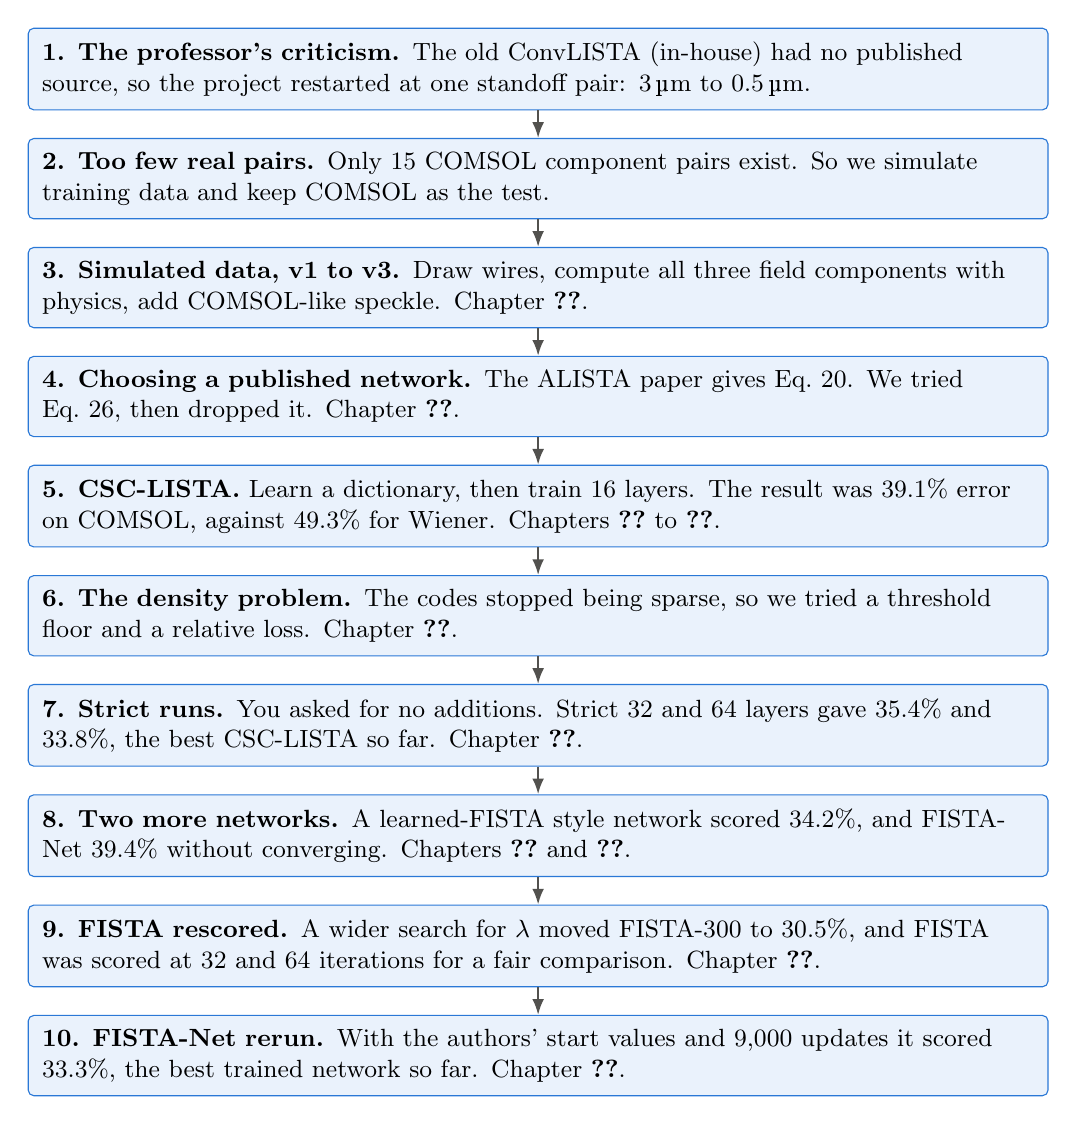
\begin{tikzpicture}[node distance=3.5mm,
  stage/.style={draw=accent,fill=bluewash,rounded corners=2pt,text width=12.6cm,inner sep=5pt,font=\small},
  arrow/.style={-{Latex[length=2mm]},draw=ink,thick}]
\node[stage] (a) {\textbf{1. The professor's criticism.} The old ConvLISTA (in-house) had no published source, so the
project restarted at one standoff pair: 3\um\ to 0.5\um.};
\node[stage,below=of a] (b) {\textbf{2. Too few real pairs.} Only 15 COMSOL component pairs exist.
So we simulate training data and keep COMSOL as the test.};
\node[stage,below=of b] (c) {\textbf{3. Simulated data, v1 to v3.} Draw wires, compute all three field
components with physics, add COMSOL-like speckle. Chapter~\ref{ch:simulation}.};
\node[stage,below=of c] (d) {\textbf{4. Choosing a published network.} The ALISTA paper gives Eq.~20. We tried Eq.~26,
then dropped it. Chapter~\ref{ch:choice}.};
\node[stage,below=of d] (e) {\textbf{5. CSC-LISTA.} Learn a dictionary, then train 16 layers. The result was
39.1\% error on COMSOL, against 49.3\% for Wiener. Chapters~\ref{ch:csc_lista} to~\ref{ch:training}.};
\node[stage,below=of e] (f) {\textbf{6. The density problem.} The codes stopped being sparse, so we tried a threshold
floor and a relative loss. Chapter~\ref{ch:density}.};
\node[stage,below=of f] (g) {\textbf{7. Strict runs.} You asked for no additions. Strict 32 and 64 layers gave
35.4\% and 33.8\%, the best CSC-LISTA so far. Chapter~\ref{ch:results}.};
\node[stage,below=of g] (h) {\textbf{8. Two more networks.} A learned-FISTA style network scored 34.2\%, and FISTA-Net
39.4\% without converging. Chapters~\ref{ch:lfista} and~\ref{ch:fistanet}.};
\node[stage,below=of h] (i) {\textbf{9. FISTA rescored.} A wider search for $\lambda$ moved FISTA-300 to 30.5\%, and FISTA was scored
at 32 and 64 iterations for a fair comparison. Chapter~\ref{ch:results}.};
\node[stage,below=of i] (j) {\textbf{10. FISTA-Net rerun.} With the authors' start values and 9,000 updates it scored 33.3\%, the best
trained network so far. Chapter~\ref{ch:fistanet}.};
\foreach \x/\y in {a/b,b/c,c/d,d/e,e/f,f/g,g/h,h/i,i/j} \draw[arrow] (\x) -- (\y);
\end{tikzpicture}
\end{center}

\section*{The result in one sentence}

FISTA at 300 iterations, a classical algorithm with no trained layers, scores 30.5\% on COMSOL. The best trained network,
FISTA-Net, scores 33.3\%, and strict Eq.~20 at 64 layers scores 33.8\%. All of them beat the Wiener filter's 49.3\% by a wide
margin, and every score here is an error, so lower is better.

\section*{How to use this booklet}

\begin{itemize}
\item \textbf{Blue boxes} hold the idea to remember.
\item \textbf{Orange boxes} hold a trap or an honest limit.
\item \textbf{Green boxes} hold what to say if your professor pushes on that point.
\item \textbf{Grey code blocks} are copied from the repository, unchanged, apart from
\texttt{\# ...} where lines are skipped. The file name is above each block.
\end{itemize}

If you only have an hour, read Chapters~\ref{ch:problem}, \ref{ch:density}, \ref{ch:results}
and~\ref{ch:defence}.

\begin{careful}[The numbers in this edition]
All server runs have finished, so every table now holds a real score. Each run used one random seed. No number here
is a prediction.
\end{careful}

\chapter{The problem, from zero}\label{ch:problem}

\section{What we are trying to do}

A Quantum Diamond Microscope measures the magnetic field above a chip. The sensor cannot touch
the wires. It sits some distance above them, and that distance is the \textbf{standoff}. The
further away you measure, the blurrier the field looks.

Our task has one sentence: given the field measured at 3\um, compute the field at 0.5\um.

We have images of size $1400\times1400$ with pixels of 0.1\um, so each image covers
$140\times140$\um. Each measurement has three components, $B_x$, $B_y$ and $B_z$. We treat
each component as a separate grey image.

\section{Why height causes blur}

Above the wires there are no currents, so the field obeys a very strict law. If you take the
2D Fourier transform of a field component at height $z$, each spatial frequency $f$ shrinks
with height by a known factor:
\begin{equation}
\widehat{B}(f,\,z+\Delta z) = \widehat{B}(f,\,z)\; e^{-2\pi |f|\,\Delta z}.
\end{equation}
This is called \textbf{upward continuation}. Fast ripples ($f$ large) die quickly. Slow, broad
shapes ($f$ small) survive. That is exactly what blur looks like.

For us, $\Delta z = 3 - 0.5 = 2.5$\um. So the blur is a known filter:
\begin{equation}
h(f) = e^{-2\pi |f| \cdot 2.5}.
\end{equation}
In the code this is one line. Everything later in this booklet calls this function.

\begin{code*}{csc_lista.py}
def transfer(n, dx, dz, dtype=torch.float32, device='cpu'):
    """The exact upward-continuation filter exp(-2 pi |f| dz) in rfft layout."""
    fy = torch.fft.fftfreq(n, dx, dtype=dtype, device=device)[:, None]
    fx = torch.fft.rfftfreq(n, dx, dtype=dtype, device=device)[None, :]
    return torch.exp(-2 * torch.pi * dz * torch.hypot(fx, fy))
\end{code*}

\begin{keyidea}[The forward model]
If $t$ is the sharp field at 0.5\um\ and $b$ is the field we measure at 3\um, then
\begin{equation}
b = h * t + \text{noise}.
\end{equation}
The star means convolution. In Fourier space it is just multiplication by $h(f)$. We know $h$
exactly, because it comes from physics. It is not learned anywhere in this project.
\end{keyidea}

\section{Why you cannot simply divide}

If $b = h\cdot t$ in Fourier space, why not compute $t = b / h$? Look at the numbers in
Figure~\ref{fig:filters}. A pattern with a 2\um\ period keeps only 0.039\% of its strength at
this standoff. Dividing multiplies by about 2,600. A pattern with a 1\um\ period is multiplied by
about 6.6 million. Any tiny noise at those frequencies becomes huge.

\begin{figure}[H]
\centering
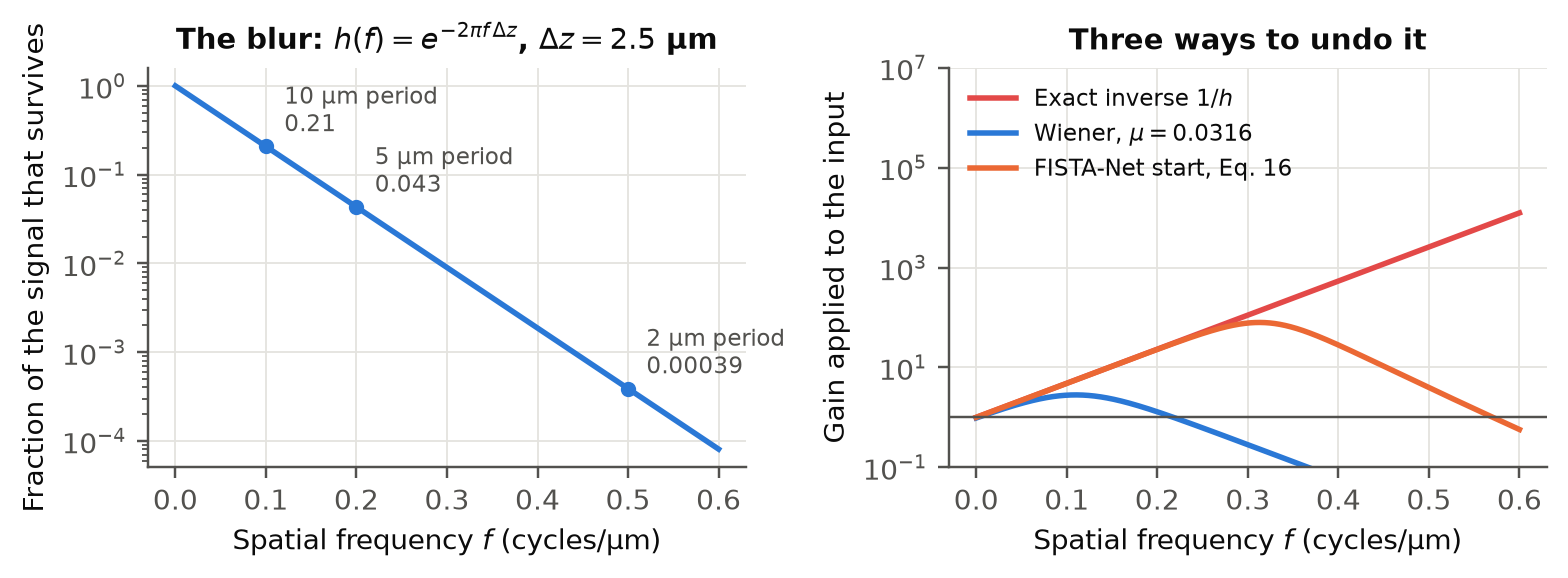
\includegraphics[width=\textwidth]{filters}
\caption{Left: how much of each frequency survives 2.5\um\ of standoff. Right: the gain three
methods apply to undo it. The red line is pure division. The blue and orange lines are the
Wiener filter and FISTA-Net's starting image, which you will meet in
Chapters~\ref{ch:classics} and~\ref{ch:fistanet}.}
\label{fig:filters}
\end{figure}

This kind of problem is called \textbf{ill-posed}. The measurement alone does not determine the
answer, so a method must add some extra belief about what fields look like. Every method in this
booklet differs mainly in what that extra belief is:

\begin{center}
\begin{tabular}{ll}
\toprule
Method & Extra belief \\
\midrule
Wiener & High frequencies are not worth trusting \\
ISTA, FISTA & The field is built from a few pieces of a dictionary \\
CSC-LISTA & Same, plus whatever training data teaches each layer \\
FISTA-Net & A small CNN learns what clean fields look like \\
\bottomrule
\end{tabular}
\end{center}

\section{How we score a result}\label{sec:score}

\textbf{Relative $L_2$ error} is the main number:
\begin{equation}
\text{error} = \frac{\lVert y - t \rVert_2}{\lVert t \rVert_2}.
\end{equation}
Here $y$ is our output and $t$ is the true field. An error of 0\% is perfect. If you output a
blank image, you score exactly 100\%. For scale, the blurry input itself scores about 77\% on the
crop shown in Figure~\ref{fig:reconstruction}.

\begin{code*}{train_csc_lista.py}
def relative_l2(output, target):
    dims = (-2, -1)
    return torch.linalg.vector_norm(output - target, dim=dims) / torch.linalg.vector_norm(target, dim=dims)
\end{code*}

\textbf{NRMSE} is the second number: the root mean square error divided by the range of the
target. It looks much smaller, about 2--4\%, because the range of these fields is large compared
with their typical value. It is the same quality of result on a friendlier scale, so never
compare an NRMSE with a relative $L_2$.

\section{The 15 test pairs}

Our test data is COMSOL, the finite-element simulation. There are five coil configurations:
\code{L1_C1}, \code{IC_4um}, \code{C1+C2}, \code{C1+C2+C3} and \code{C1+C2+C3+C4}. Each gives
three components at both heights, so $5\times3=15$ pairs. Each reported score is the mean over
these 15.

\begin{careful}[15 pairs are not 15 independent tests]
They contain only two wire shapes. C2, C3 and C4 are mirror copies of C1, and
\code{IC_2um} and \code{IC_4um} are the same coil. This is why the scores for different
configurations look almost identical. Say ``15 pairs from two wire shapes''.
\end{careful}

\section{The rule that protects the result}

\begin{keyidea}[COMSOL is the exam, not the homework]
Models train only on simulated data. Settings and checkpoints are picked only on simulated
validation data. COMSOL is read once, after training, to produce the final score.
\end{keyidea}

There is one honest exception, covered in Chapter~\ref{ch:results}. The generator's width range,
speckle level and wire families were designed by looking at these same COMSOL coils. No
reconstruction score leaked, but the data was designed with the exam in mind.

\chapter{Simulated data}\label{ch:simulation}

You understood this up to version 3, so this chapter moves quickly. It collects the method in
one place, because the training later depends on it.

\begin{careful}[Synthetic and simulated are two different things here]
The repository has two generators, and it is easy to mix up the words.
\begin{itemize}
\item \textbf{Synthetic data} is the earlier pipeline from October, in \code{scripts/synthetic_data.py}. It makes new pairs by
augmenting real COMSOL fields. It was used for the 1,080-pair experiment, and it is \emph{not} used here.
\item \textbf{Simulated data} is the new generator, \code{scripts/simulate_fields.py}. It computes fields from drawn
wires, and COMSOL never enters it. Everything in this booklet uses simulated data, version 3.
\end{itemize}
\end{careful}

\section{Why simulate at all}

Fifteen pairs from two wire shapes cannot train a network with millions of parameters. So we
need many more examples of the same physics. Your original idea was a spiral with blur and noise.
The final generator goes one step further: it computes the field from a current, so all three
components agree with each other and with Maxwell's equations. This is much easier to defend than
a blurred line drawing.

\section{The recipe, step by step}

\subsection*{Step 1: draw a wire layout}

Each sample starts from a recipe. It picks a family and random settings.

\begin{code*}{simulate_fields.py}
    rng = np.random.default_rng(sample_seed(seed, label))
    family = str(rng.choice(('spiral', 'meander', 'array'), p=(.35, .35, .3)))
    width = float(rng.uniform(*settings['width_um']))
\end{code*}

\begin{itemize}
\item \textbf{Spiral:} a two-arm rectangular spiral, like L1\_C1.
\item \textbf{Meander:} a serpentine with uneven teeth.
\item \textbf{Array:} 2 to 4 mirror copies of one spiral in the image quadrants, like C1+C2+C3+C4.
\end{itemize}

Every path is closed. It leaves the image and returns along a rail 35\um\ outside, because real
current must flow in a loop. The code redraws a layout if any wires come too close. Each sample also
gets a random width of 1.6--3.2\um, a source offset of 0--0.2\um, and a noise level of 1, 1.5, 2 or
2.5\%. The current is fixed at 600\textmu A, the same as COMSOL.

\subsection*{Step 2: turn the wire into a current map}

\code{rasterize} paints the wire onto a pixel grid as two arrays, $K_x$ and $K_y$, the sheet current
density in A/m. It uses partial pixel coverage so edges are not jagged. At a corner two wires overlap,
so the current there is shared equally.

\begin{code*}{simulate_fields.py}
    # Both wires cover a corner square; share the current between them there.
    corner = (kx != 0) & (ky != 0)
    kx[corner] /= 2
    ky[corner] /= 2
\end{code*}

The canvas has 700 pixels of padding on each side, so the Fourier transform does not wrap
fields around the image edges.

\subsection*{Step 3: compute the field from the current}

This is the thin-sheet Biot--Savart law in Fourier space. With $k=2\pi|f|$ and $d$ the source offset:
\begin{align}
E(k,z) &= \frac{\mu_0}{2}\, e^{-k(z+d)},\\
B_x(k) &= E\, K_x(k),\\
B_y(k) &= E\, K_y(k),\\
B_z(k) &= E\, \frac{i\,(k_y K_x(k) - k_x K_y(k))}{k}.
\end{align}

\begin{code*}{simulate_fields.py}
    fx, fy = np.fft.rfft2(kx), np.fft.rfft2(ky)
    # Drawn corners leak a little current; remove the divergent part so the
    # in-plane fields describe the same conserved current as Bz.
    longitudinal = (wx * fx + wy * fy) / safe ** 2
    fx, fy = fx - wx * longitudinal, fy - wy * longitudinal
    fz = 1j * (wy * fx - wx * fy) / safe
    fx[0, 0] = fy[0, 0] = fz[0, 0] = 0
\end{code*}

Notice that one current map gives all three components at both heights. Nothing is drawn separately.

\begin{keyidea}[The target and the input come from the same physics]
The same formula runs twice, at $z=0.5$ and $z=3$. So the training pair is consistent with the
operator $h$ by construction.
\end{keyidea}

\begin{careful}[The labels look swapped, and that is deliberate]
In real physics, $B_x$ is driven by $K_y$. Here $B_x$ uses $K_x$. That is because the COMSOL
export frame is rotated 90 degrees from the image axes. Bx and By only satisfy Maxwell's
equations with Bz when the frame is rotated: the residual is 10.9\% rotated and about 100\% as
labelled. The generator copies the COMSOL frame.
\end{careful}

\subsection*{Step 4: add COMSOL-like noise, to the input only}

COMSOL fields carry a fine speckle tied to the mesh. Measured from mirrored coils, it has a range of
1.4--1.9\% for $B_x$ and $B_y$, 2--3.4\% for $B_z$, and a correlation length of about 0.38\um. So the
generator adds noise that is correlated over that same length.

\begin{code*}{simulate_fields.py}
def correlated_noise(white, corr_um, dx):
    """Unit-variance noise with exponential spatial correlation length corr_um."""
    ny, nx = white.shape
    fx = np.fft.rfftfreq(nx, dx)[None, :]
    fy = np.fft.fftfreq(ny, dx)[:, None]
    f2 = fx ** 2 + fy ** 2
    amplitude = (1 + (2 * np.pi * corr_um) ** 2 * f2) ** -0.75
    field = np.fft.irfft2(np.fft.rfft2(white) * amplitude, s=(ny, nx))
    return (field - field.mean()) / field.std()
\end{code*}

Noise goes on the input only. The target stays clean. So the network is asked to remove speckle
as well as blur.

\subsection*{Step 5: normalise}

All fields are divided by one number: 145.487\muT, the largest peak among the training targets.
COMSOL is divided by the same number, and it never helps choose that number.

\begin{figure}[H]
\centering
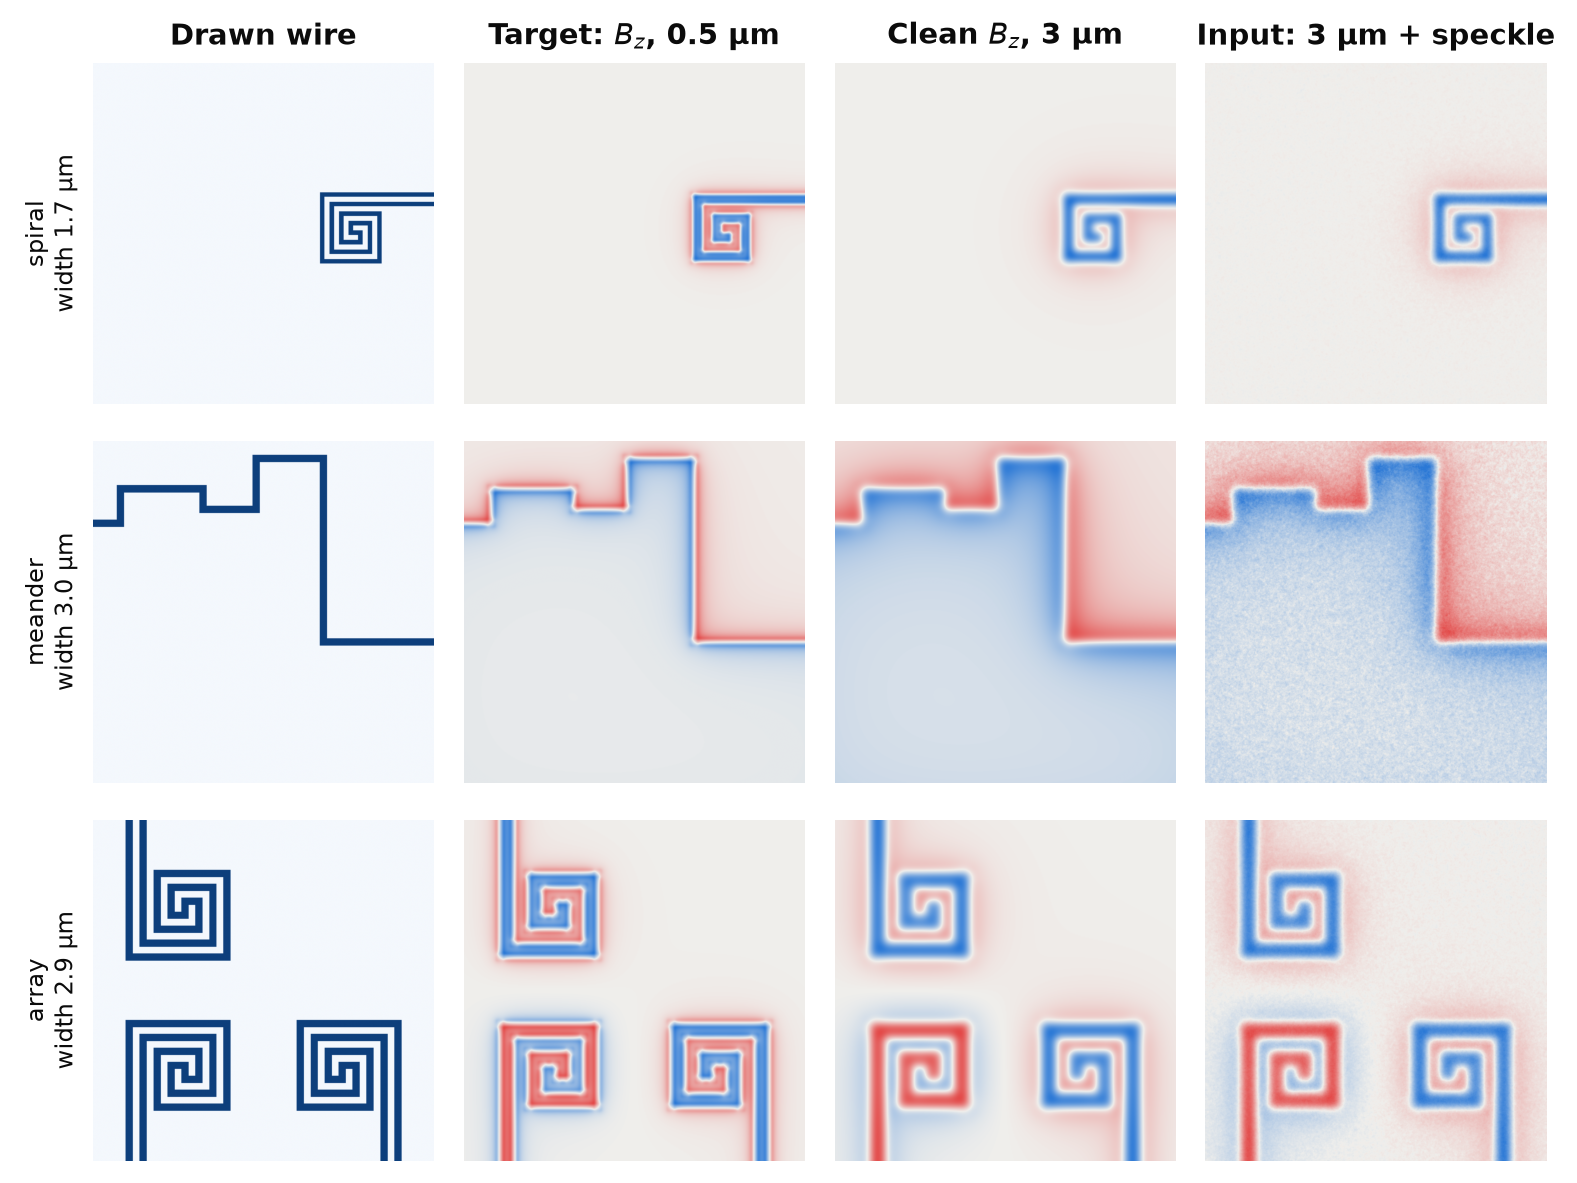
\includegraphics[width=\textwidth]{simulated}
\caption{Three training layouts from v3, one from each family. Only $B_z$ is shown. The right two
columns share a colour scale, so the speckle is visible in the input.}
\label{fig:simulated}
\end{figure}

\section{How v1 became v3}

\begin{center}
\begin{tabularx}{\textwidth}{lX}
\toprule
Version & What it had \\
\midrule
v1 & One wire per sample, free-space decay, white noise \\
v2 & Added array layouts and correlated speckle, plus an empirical decay $k_0=0.095$ rad/\textmu m
that mimics COMSOL's faster fall-off \\
v3 & Same layouts as v2, with $k_0$ removed. Pure free-space physics. This is the dataset used \\
\bottomrule
\end{tabularx}
\end{center}

\begin{keyidea}[Why $k_0$ was removed]
COMSOL fields decay faster with height than free-space physics allows, and the cause is unknown.
A term like $k_0$ fits this, but it breaks the law that a static field above its sources must
obey. You rejected it, and the operator stayed $e^{-kz}$. The mismatch is small at 3\um\ and large
by 10\um, which is one more reason to work at 3\um.
\end{keyidea}

\section{What was generated}

\begin{center}
\begin{tabular}{lr}
\toprule
Item & Value \\
\midrule
Training layouts & 200 \\
Validation layouts & 50 \\
Component pairs & 750 \\
Families & 80 spirals, 97 meanders, 73 arrays \\
Size on disk & 536 KB of recipes \\
\bottomrule
\end{tabular}
\end{center}

The dataset stores recipes, not images, and regenerates arrays when needed. The split is by
layout, so a validation wire is never seen in training.

\section{How realistic is it?}

To check the physics, the real L1\_C1 coil was rebuilt from its traced centreline and compared with
COMSOL.

\begin{center}
\begin{tabular}{lccc}
\toprule
Height & $B_x$ error & $B_y$ error & $B_z$ error \\
\midrule
0.5\um & 16.8\% & 18.8\% & 23.0\% \\
3\um & 12.7\% & 13.8\% & 25.8\% \\
10\um & 63.7\% & 64.1\% & 139.7\% \\
\bottomrule
\end{tabular}
\end{center}

So the simulator is close at our two heights and fails at 10\um.

\begin{careful}[Limits of the simulator]
\begin{itemize}
\item The wire width and offset for that check were fitted on the same coil, so it is a regression
check, not independent proof.
\item COMSOL's speckle sets a floor. Even a perfect clean model cannot score below about 15--19\%
against COMSOL at 0.5\um, because that much of the COMSOL target is mesh speckle.
\item Every COMSOL peak lies above the simulated range, so the spikes are not modelled.
\item Fifteen automated tests pass, covering closed-form loop and strip fields, Maxwell
consistency, and repeatability.
\end{itemize}
\end{careful}

\chapter{The classical methods: Wiener, ISTA, FISTA}\label{ch:classics}

Every network here is built from these three ideas, so they come first.

\section{What is Wiener?}

You asked about this directly. The Wiener filter in our tables is the simplest sensible way to undo
the blur. It involves no learning at all.

We want an image $x$ whose blurred version matches $b$, but we refuse to let $x$ get too large:
\begin{equation}
\min_x\; \lVert h * x - b \rVert_2^2 + \mu \lVert x \rVert_2^2 .
\end{equation}
The first term says ``match the measurement''. The second says ``keep it small''. In Fourier space
each frequency is a separate small problem, and setting the derivative to zero gives the answer directly:
\begin{equation}
\widehat{x}(f) = \frac{h(f)}{h(f)^2 + \mu}\; \widehat{b}(f).
\end{equation}

Look at what this does. Where $h$ is large (slow patterns), $\mu$ is negligible, so the fraction is
about $1/h$: a true inverse. Where $h$ is tiny, the fraction is about $h/\mu$, which goes to zero.
So it inverts what it can trust and gives up on the rest. The blue line in
Figure~\ref{fig:filters} shows this.

\begin{code*}{csc_lista.py}
class Dataless(nn.Module):
    """Tikhonov/Wiener baseline with the same exp(-kz) operator."""

    def __init__(self, dx, dz, mu):
        super().__init__()
        self.dx, self.dz, self.mu = dx, dz, mu

    def forward(self, b):
        n = b.shape[-1]
        h = transfer(n, self.dx, self.dz, b.dtype, b.device)
        return torch.fft.irfft2(torch.fft.rfft2(b) * h / (h * h + self.mu), s=(n, n))
\end{code*}

The only setting is $\mu$. We tried values from $10^{-6}$ to $10^{-0.5}$ in half-decade steps on
simulated validation crops, and $\mu=0.0316$ won. With this $\mu$ the largest gain is 2.8, at a
period of about 9\um. Beyond about 0.4 cycles per \textmu m its gain is below 0.1, so it has effectively given up.

Strictly, a true Wiener filter uses the signal and noise spectra. With a single constant $\mu$
this is also called \textbf{Tikhonov} regularisation. The code's docstring says both, and the
tables use the short name Wiener.

\begin{keyidea}[Why Wiener matters here]
It is the honest baseline. It knows the physics, uses no training data, and takes one line. Any network
must beat it. It scores 49.3\% on COMSOL.
\end{keyidea}

\section{Sparse coding: a better belief}

Wiener treats every frequency separately, so it cannot know that fields come from wires. Sparse
coding says something stronger: \emph{a sharp field is made of a few repeated pieces}.

Take a set of small images $g_1,\dots,g_M$, called \textbf{atoms}, or together a
\textbf{dictionary}. Stamp them at chosen positions and add them up:
\begin{equation}
t \approx \sum_{m=1}^{M} g_m * x_m .
\end{equation}
Each $x_m$ is a map the size of the image, called a \textbf{code}. Most of its values are zero, and a
nonzero value means ``stamp atom $m$ here, this strongly''.

\begin{keyidea}[The trick that puts the blur in]
We measure $b = h*t$. Substitute the sparse model for $t$:
\begin{equation}
b \approx h * \sum_m g_m * x_m = \sum_m (h * g_m) * x_m = \sum_m d_m * x_m,
\qquad d_m = h*g_m .
\end{equation}
So the \textbf{blurred} field is built from \textbf{blurred} atoms $d_m$, using the \emph{same} codes. Find
the codes from $b$ using $d$, then rebuild the sharp field using $g$. That is the whole method.
\end{keyidea}

\begin{center}
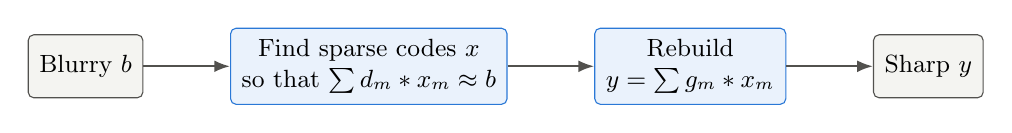
\begin{tikzpicture}[node distance=6mm and 11mm]
\node[fixed] (b) {Blurry $b$};
\node[block,right=of b] (solve) {Find sparse codes $x$\\ so that $\sum d_m*x_m\approx b$};
\node[block,right=of solve] (rebuild) {Rebuild\\ $y=\sum g_m*x_m$};
\node[fixed,right=of rebuild] (y) {Sharp $y$};
\draw[flow] (b) -- (solve);
\draw[flow] (solve) -- (rebuild);
\draw[flow] (rebuild) -- (y);
\end{tikzpicture}
\end{center}

To find the codes, we solve the \textbf{Lasso}:
\begin{equation}
\min_x\; \tfrac12 \Big\lVert \sum_m d_m*x_m - b \Big\rVert_2^2 + \lambda \lVert x \rVert_1 .
\end{equation}
The first term matches the measurement. The second, the $\ell_1$ penalty, pushes values to exactly
zero. A larger $\lambda$ gives sparser codes and a worse fit.

\section{ISTA}

ISTA solves the Lasso by repeating two simple moves. Write $D$ for the operator
$x\mapsto\sum_m d_m*x_m$ and $D^T$ for its transpose.

\begin{equation}
x^{(k+1)} = \soft_{\lambda/L}\!\left( x^{(k)} - \frac1L D^T\big(Dx^{(k)} - b\big) \right).
\end{equation}

\begin{enumerate}
\item \textbf{Gradient step.} $Dx-b$ is the current mismatch. $D^T$ carries it back to code space. We
step downhill by $1/L$. $L$ must be at least the largest eigenvalue of $D^TD$, or the iteration can
blow up.
\item \textbf{Shrink.} The function $\soft_\theta$ moves every value toward zero by $\theta$, and small values
land exactly on zero. This is where sparsity comes from.
\end{enumerate}

\begin{minipage}{.5\textwidth}
\begin{code*}{csc_lista.py}
def shrink(x, theta):
    return torch.sign(x) * torch.relu(torch.abs(x) - theta)
\end{code*}
\end{minipage}\hfill
\begin{minipage}{.44\textwidth}
\centering
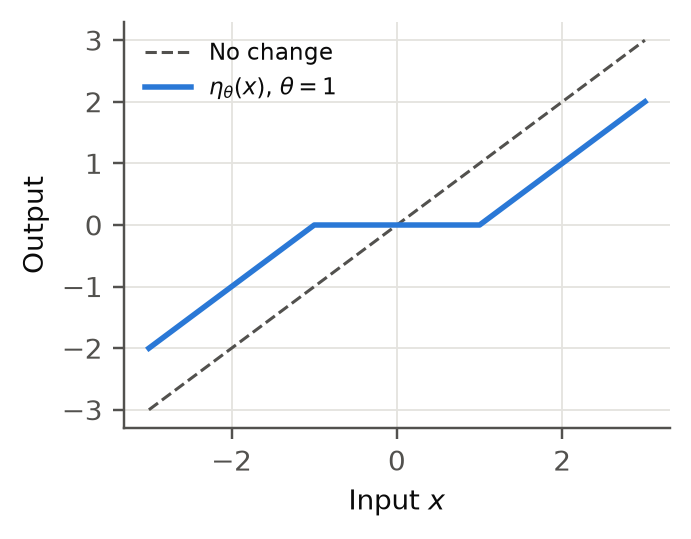
\includegraphics[width=\linewidth]{shrink}
\captionof{figure}{Soft thresholding. Anything within $\pm\theta$ becomes zero.}
\end{minipage}

\medskip
In formula form, $\soft_\theta(x)=\sign(x)\max(|x|-\theta,0)$. The code is that formula.

\section{FISTA}

ISTA is slow. FISTA adds one small idea, momentum. It takes the gradient step not from the
current point, but from a point pushed further along the direction it was already moving:
\begin{align}
x^{(k)} &= \soft_{\lambda/L}\!\left( y^{(k)} - \tfrac1L D^T(Dy^{(k)} - b) \right),\\
t_{k+1} &= \tfrac12\big(1+\sqrt{1+4t_k^2}\big),\\
y^{(k+1)} &= x^{(k)} + \frac{t_k-1}{t_{k+1}}\big(x^{(k)}-x^{(k-1)}\big).
\end{align}
The cost per step is the same, but the convergence rate improves from $O(1/k)$ to $O(1/k^2)$. Our code holds
both algorithms in one function, with \code{fast} choosing between them:

\begin{code*}{csc_lista.py}
def code_ista(b, operator, lam, steps, pad=0, fast=True, bound=None):
    """FISTA or ISTA for 0.5 ||mask(Dx - b)||^2 + lam ||x||_1."""
    n = b.shape[-1]
    mask = window_mask(n, pad, b.device) if pad else 1.0
    step = 1 / (bound or operator.bound(n))
    x = torch.zeros(b.shape[0], operator.filters.shape[0], n, n, dtype=b.dtype,
                    device=b.device)
    y, t = x, 1.0
    for _ in range(steps):
        residual = mask * (operator.forward(y) - b)
        update = shrink(y - step * operator.adjoint(residual), lam * step)
        if fast:
            t_next = (1 + (1 + 4 * t * t) ** .5) / 2
            y = update + (t - 1) / t_next * (update - x)
            t = t_next
        else:
            y = update
        x = update
    return x
\end{code*}

\section{How well do they do?}

Both use the same dictionary as the networks. FISTA's $\lambda$ was picked on 16 simulated validation crops. The first
search tried 0.03, 0.09, 0.3 and 0.9, and the smallest won. That is the edge of the grid, so the search was widened, and
$\lambda=0.009$ won with worse values on both sides. Chapter~\ref{ch:results} shows the full search.

\begin{center}
\begin{tabular}{lcc}
\toprule
Method & Simulated validation & COMSOL \\
\midrule
ISTA, 16 iterations & 64.3\% & 64.4\% \\
FISTA, 32 iterations & 50.9\% & 41.8\% \\
FISTA, 64 iterations & 45.3\% & 37.9\% \\
FISTA, 300 iterations, $\lambda=0.03$ & 36.6\% & 32.1\% \\
FISTA, 300 iterations, $\lambda=0.009$ & 35.5\% & 30.5\% \\
\bottomrule
\end{tabular}
\end{center}

\begin{keyidea}[Read this table carefully]
ISTA with 16 steps is awful because it has barely started. FISTA with 300 steps is the best thing in
the whole project so far. So the sparse model itself is good, and the problem is speed. This is exactly
what learned networks were invented to fix: reach a similar answer in far fewer steps.
\end{keyidea}

\chapter{Choosing a published architecture}\label{ch:choice}

\section{The idea of unrolling}

Picture ISTA as a pipeline. One iteration is one box, so $K$ iterations are $K$ boxes in a row. Each box
contains fixed numbers: $D^T/L$ and $\lambda/L$. Now stop treating those numbers as fixed. Make them
trainable, one set per box, and train the whole chain by backpropagation. A loop has become a
neural network.

\begin{center}
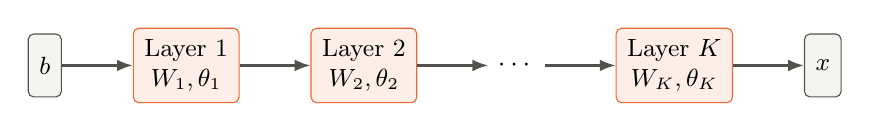
\begin{tikzpicture}[node distance=9mm]
\node[fixed] (b) {$b$};
\node[learned,right=of b] (l1) {Layer 1\\ $W_1,\theta_1$};
\node[learned,right=of l1] (l2) {Layer 2\\ $W_2,\theta_2$};
\node[right=of l2] (dots) {$\cdots$};
\node[learned,right=of dots] (lk) {Layer $K$\\ $W_K,\theta_K$};
\node[fixed,right=of lk] (x) {$x$};
\draw[flow] (b)--(l1); \draw[flow] (l1)--(l2); \draw[flow] (l2)--(dots);
\draw[flow] (dots)--(lk); \draw[flow] (lk)--(x);
\end{tikzpicture}
\end{center}

This is \textbf{LISTA}, by Gregor and LeCun (2010). It is written in the ALISTA paper as:
\begin{equation}
x^{(k+1)} = \soft_{\theta^{(k)}}\big(W_1^{(k)} b + W_2^{(k)} x^{(k)}\big). \tag{Liu et al., Eq.~4}
\end{equation}
Setting $W_1=D^T/L$, $W_2=I-D^TD/L$ and $\theta=\lambda/L$ gives back ISTA exactly. So LISTA starts as
ISTA and can only be taught to improve.

\section{Why plain LISTA cannot run here}

$W$ is a full matrix. An image has 1.96 million pixels, so such a matrix would have about
$4\times10^{12}$ entries, and that is for a single pixel-to-pixel map. The earlier dense ALISTA code in
the repository stays as it is, but it cannot run at 0.1\um.

There is a way out. The blur is the same everywhere in the image. So we can use convolutions, which
reuse one small filter at every position. This leads to \textbf{convolutional sparse coding}.

\section{The ALISTA paper}

Liu, Chen, Wang and Yin, ``ALISTA: Analytic Weights Are As Good As Learned Weights in LISTA'', ICLR
2019. It has two main messages.

\begin{enumerate}
\item \textbf{Analysis.} The weights of LISTA do not all need to be learned. A single weight
matrix can be computed from $D$ by a formula. Only step sizes and thresholds then need training.
\item \textbf{Extension.} Section 3 carries all of this to convolutions.
\end{enumerate}

Section 3 starts with the convolutional model, Eq.~17:
\begin{equation}
b = \sum_{m=1}^{M} d_m * x_m^* + \varepsilon . \tag{Liu et al., Eq.~17}
\end{equation}
This is the same equation as our $b\approx\sum_m d_m*x_m$. Then the paper gives the two networks.

\begin{center}
\renewcommand{\arraystretch}{1.5}
\begin{tabularx}{\textwidth}{l>{\raggedright\arraybackslash}X>{\raggedright\arraybackslash}X}
\toprule
& \textbf{Eq.~20: CSC-LISTA} & \textbf{Eq.~26: Conv ALISTA} \\
\midrule
Update &
$x_m \leftarrow \soft_{\theta^{(k)}}\!\big(x_m - (w_m^{(k)})' * (\sum_{\bar m} d_{\bar m}*x_{\bar m} - b)\big)$ &
$x_m \leftarrow \soft_{\theta^{(k)}}\!\big(x_m - \gamma_m^{(k)} \tilde w_m' * (\sum_{\bar m} d_{\bar m}*x_{\bar m} - b)\big)$ \\
Filters & $w_m^{(k)}$ learned, one set per layer & $\tilde w_m$ fixed, computed by formula \\
Trained & All filters and thresholds & Only $\gamma$ and $\theta$ \\
Parameters here & 24.6 million at 32 layers & About a thousand at 32 layers \\
\bottomrule
\end{tabularx}
\end{center}

The prime means a filter rotated by 180 degrees. Think of it as the convolutional version of a
matrix transpose.

\section{Why Eq.~20 and not Eq.~26}

This choice was made during the session, for these reasons:

\begin{enumerate}
\item \textbf{The paper itself reports a small gap.} Its Appendix H denoising test gives Eq.~20 (the paper's ``Conv LISTA'', our CSC-LISTA) an
average PSNR of 31.21 dB and Conv ALISTA 31.07 dB. Learned filters are not worse.
\item \textbf{The analytic filters behaved badly on our blur.} In a small spike, the analytic weight
acted almost like an inverse filter and amplified noise by hundreds of times or more. That spike used
the field itself as the code, with one filter, which is not the model of Chapter~\ref{ch:classics}. Its
code was deleted at your request, so treat this as a note from the session, not a reproducible result.
\item \textbf{You chose.} You told me to drop Eq.~26 and remove everything related to it, so that it
could not cause confusion later. The old dense ALISTA code stayed, also by your choice.
\end{enumerate}

\begin{careful}[The theory does not cover us]
The paper proves fast convergence when the true code is very sparse. For our blur kernel, that limit
worked out to about 1--2 active pixels, while the coil images have tens of thousands or more. So do not claim the
convergence theorems apply here. Use the paper for its architecture, not for its guarantee.
\end{careful}

\section{Other options considered}

\begin{center}
\begin{tabularx}{\textwidth}{lX}
\toprule
Option & Status \\
\midrule
USRNet, ISTA-Net, MoDL & Discussed earlier as published unrolled networks. Not built \\
LFISTA (Moreau and Bruna) & Dense form cannot run. A convolutional relative is Job 3,
Chapter~\ref{ch:lfista} \\
FISTA-Net (Xiang et al.) & You supplied this paper. It is Job 4, Chapter~\ref{ch:fistanet} \\
\bottomrule
\end{tabularx}
\end{center}

\begin{defend}
\textbf{``Where does this network come from?''} The layer is Eq.~20 of Liu et al., ICLR 2019, and
convolutional sparse coding is an established field. What is ours is using it for deblurring, by
writing $d_m=h*g_m$. The paper's own experiment is denoising, so no published result exists for this exact
use. Say this before you are asked.
\end{defend}

\chapter{CSC-LISTA: the architecture}\label{ch:csc_lista}

This chapter goes through the network piece by piece, and checks each piece against Eq.~20.

\section{The equation}

Eq.~20 of Liu et al., for layer $k$ and atom $m$:
\begin{equation}
x_m^{(k+1)} = \soft_{\theta^{(k)}}\!\left( x_m^{(k)} - \big(w_m^{(k)}\big)' *
\Big( \sum_{\bar m=1}^{M} d_{\bar m} * x_{\bar m}^{(k)} - b \Big) \right). \tag{Liu et al., Eq.~20}
\end{equation}

Read it from the inside out, in plain words:

\begin{enumerate}
\item $\sum d_{\bar m}*x_{\bar m}$: blur the current codes back into a predicted measurement.
\item Subtract $b$: this is the mismatch, also called the \textbf{residual}.
\item $(w_m)'*$: pass the residual through a learned filter, once per atom. This turns one image of
mismatch into 32 maps of correction.
\item Subtract the correction from $x_m$.
\item $\soft_\theta$: shrink, so that small values become zero.
\end{enumerate}

Compare it with ISTA. There, $(w_m)'$ is fixed at $d_m'/L$. So the entire change in Eq.~20 is that
\emph{each layer gets to learn its own correction filter and its own threshold}.

\section{Everything in one picture}

\begin{figure}[H]
\centering
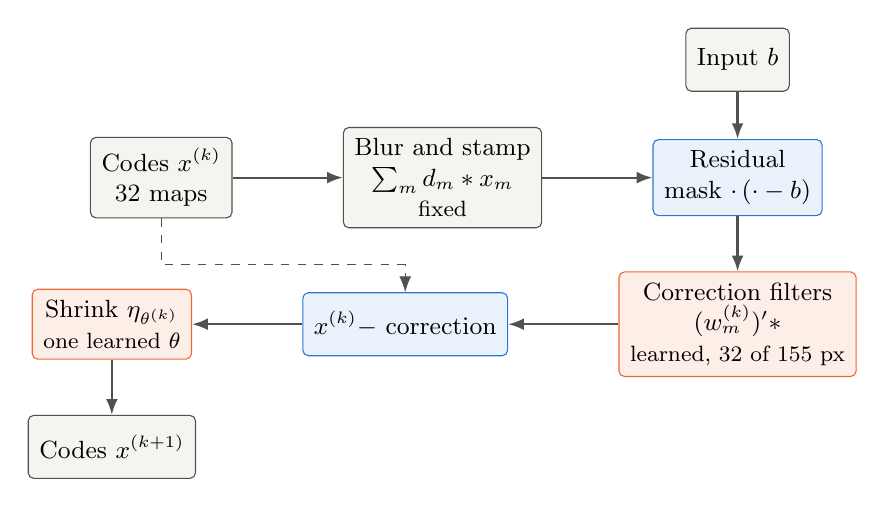
\begin{tikzpicture}[node distance=7mm and 9mm]
\node[fixed] (x) {Codes $x^{(k)}$\\ 32 maps};
\node[fixed,right=14mm of x] (D) {Blur and stamp\\ $\sum_m d_m*x_m$\\ \footnotesize fixed};
\node[block,right=14mm of D] (r) {Residual\\ mask $\cdot\,(\cdot-b)$};
\node[learned,below=of r] (w) {Correction filters\\ $(w_m^{(k)})'*$\\ \footnotesize learned, 32 of 155 px};
\node[block,left=14mm of w] (sub) {$x^{(k)} -$ correction};
\node[learned,left=14mm of sub] (s) {Shrink $\soft_{\theta^{(k)}}$\\ \footnotesize one learned $\theta$};
\node[fixed,below=of s] (next) {Codes $x^{(k+1)}$};
\node[fixed,above=6mm of r] (b) {Input $b$};
\draw[flow] (x)--(D); \draw[flow] (D)--(r); \draw[flow] (b)--(r);
\draw[flow] (r)--(w); \draw[flow] (w)--(sub); \draw[flow] (sub)--(s); \draw[flow] (s)--(next);
\draw[dashflow] (x.south) |- ($(sub.north)+(0,3.5mm)$) -- (sub.north);
\end{tikzpicture}
\caption{One CSC-LISTA layer. Orange boxes are learned. Grey boxes are fixed. After the final layer,
the output field is $\sum_m g_m * x_m^{(K)}$.}
\label{fig:layer}
\end{figure}

\section{The sizes of everything}

\begin{center}
\begin{tabular}{llp{6.7cm}}
\toprule
Object & Shape & Meaning \\
\midrule
\code{b} & $[B, N, N]$ & Batch of padded input images \\
\code{x} & $[B, 32, N, N]$ & 32 code maps per image, one per atom \\
\code{atoms} & $[32, 75, 75]$ & Sharp dictionary $g_m$, 7.5\um\ wide, fixed \\
\code{w} & $[K, 32, 155, 155]$ & Learned filters, 15.5\um\ wide \\
\code{theta} & $[K]$ & One threshold per layer \\
\bottomrule
\end{tabular}
\end{center}

During training $N=768$, which is a 512 pixel crop plus 128 pixels of padding on each side. On a
full image $N=1656$. The same weights work at both sizes, because the network is convolutional.

The parameter count comes straight from these shapes:
\begin{equation}
K \times (155^2 \times 32) + K .
\end{equation}
This gives 12,300,816 at 16 layers, 24,601,632 at 32, and 49,203,264 at 64. Those numbers match
the saved run files.

\section{The code, line by line}

\subsection*{The operator: convolving with many filters using FFTs}

A 75 pixel filter convolved directly on a $768\times768$ image would be far too slow, and the blur
$h$ is defined in Fourier space anyway. So every convolution is done as a multiplication of spectra.
\code{Operator} wraps this.

\begin{code*}{csc_lista.py}
class Operator:
    """A convolutional dictionary, optionally followed by the standoff filter h.

    Spectra are built on demand and `chunk` filters at a time, so a full image
    never holds every filter spectrum in memory at once.
    """

    def __init__(self, filters, h=None, chunk=None):
        self.filters, self.h = filters, h
        self.chunk = chunk or filters.shape[0]

    def spectra(self, n):
        for first in range(0, self.filters.shape[0], self.chunk):
            part = centred_rfft(self.filters[first:first + self.chunk], n)
            yield first, part if self.h is None else part * self.h
\end{code*}

Look at the last line. If \code{h} is given, each filter's spectrum is multiplied by $h$. \textbf{That
single multiplication is $d_m=h*g_m$.} The same class is the sharp dictionary $G$ when \code{h} is
\code{None}, and the blurred dictionary $D$ when \code{h} is set.

\begin{code*}{csc_lista.py}
    def forward(self, x):
        """sum_m filter_m * x_m for maps [B, M, N, N]; returns [B, N, N]."""
        n = x.shape[-1]
        total = 0
        for first, part in self.spectra(n):
            total = total + (torch.fft.rfft2(x[:, first:first + part.shape[0]]) * part).sum(1)
        return torch.fft.irfft2(total, s=(n, n))

    def adjoint(self, residual):
        """filter_m' * residual, the transpose of forward, for [B, N, N] input."""
        n = residual.shape[-1]
        spectrum = torch.fft.rfft2(residual)[:, None]
        return torch.cat([torch.fft.irfft2(spectrum * part.conj(), s=(n, n))
                          for _, part in self.spectra(n)], 1)
\end{code*}

\code{forward} is $\sum_m f_m*x_m$: many maps go in, one image comes out. \code{adjoint} goes the
other way: one image goes in, 32 maps come out.

\begin{keyidea}[Why \texttt{part.conj()} is the 180-degree rotation]
Eq.~20 needs $(w_m)'$, the filter rotated by 180 degrees. For a real filter, rotating by 180 degrees in
space is the same as taking the complex conjugate in Fourier space. So \code{part.conj()} is exactly the prime in
the equation. A unit test confirms that \code{forward} and \code{adjoint} are true transposes.
\end{keyidea}

\subsection*{The largest eigenvalue $L$}

\begin{code*}{csc_lista.py}
    def bound(self, n):
        """Largest eigenvalue of D D^T on an n-square canvas."""
        return float(sum((part.abs() ** 2).sum(0) for _, part in self.spectra(n)).max())
\end{code*}

In Fourier space the operator splits into small independent pieces, one per frequency. So the
largest eigenvalue is simply the largest value of $\sum_m|D_m(f)|^2$ over all frequencies. For our
dictionary, $L\approx77{,}633$.

\subsection*{The starting point: the network begins as ISTA}

\begin{code*}{csc_lista.py}
        h = transfer(canvas, dx, dz, atoms.dtype, atoms.device)
        operator = Operator(atoms, h, chunk)
        step = 1 / operator.bound(canvas)
        self.bound_value = 1 / step
        # ISTA start: w = d / L, truncated to the filter support.
        rows = []
        for first, part in operator.spectra(canvas):
            full = torch.roll(torch.fft.irfft2(part, s=(canvas, canvas)),
                              (width // 2, width // 2), (-2, -1))
            rows.append(full[..., :width, :width] * step)
        self.w = nn.Parameter(torch.cat(rows)[None].repeat(layers, 1, 1, 1))
        self.theta = nn.Parameter(torch.full((layers,), lam * step, dtype=atoms.dtype,
                                             device=atoms.device))
\end{code*}

Each $w$ starts as $d_m/L$, cut to 155 pixels, and each threshold starts at $\lambda/L$. All layers
start identical. So before training the network \emph{is} ISTA, apart from the cut. A test confirms this: with
filters wide enough, the untrained network matches ISTA to within 2\%.

\subsection*{One layer}

Here is Eq.~20 in the code. Compare it with the equation, term by term.

\begin{code*}{csc_lista.py}
    def layer(self, x, b, k, operator, mask):
        residual = mask * (operator.forward(x) - b)
        update = x - Operator(self.w[k], chunk=self.chunk).adjoint(residual)
        return shrink(update, self.theta[k].clamp_min(0))
\end{code*}

\begin{center}
\renewcommand{\arraystretch}{1.5}
\begin{tabular}{p{5.1cm}p{9.4cm}}
\toprule
Paper & Code \\
\midrule
$\sum_{\bar m} d_{\bar m}*x_{\bar m}$ & \code{operator.forward(x)} \\
$\sum_{\bar m} d_{\bar m}*x_{\bar m} - b$ & \code{mask * (operator.forward(x) - b)} \\
$(w_m^{(k)})' * (\cdot)$ & \code{Operator(self.w[k], ...).adjoint(residual)} \\
$x_m^{(k)} - (\cdot)$ & \code{update = x - ...} \\
$\soft_{\theta^{(k)}}(\cdot)$ & \code{shrink(update, self.theta[k].clamp_min(0))} \\
Sum over $m=1\dots M$ & Handled by the tensor shapes \\
\bottomrule
\end{tabular}
\end{center}

Two small things in that code are not in the equation: the \code{mask} and the \code{clamp_min(0)}.
Both are listed in Chapter~\ref{ch:differences}.

\subsection*{All the layers, and the output}

\begin{code*}{csc_lista.py}
    def codes(self, b):
        n = b.shape[-1]
        operator, mask = self.physics(n)
        x = torch.zeros(b.shape[0], self.w.shape[1], n, n, dtype=b.dtype, device=b.device)
        y = x
        for k in range(self.layers):
            if self.use_checkpoint and self.training:
                update = checkpoint(self.layer, y, b, k, operator, mask, use_reentrant=False)
            else:
                update = self.layer(y, b, k, operator, mask)
            y = update if self.beta is None else update + self.beta[k] * (update - x)
            x = update
        return x
\end{code*}

Codes start at zero. For Eq.~20 runs \code{self.beta} is \code{None}, so \code{y} is simply the latest
\code{update}. The momentum line matters only in Chapter~\ref{ch:lfista}.

\code{checkpoint} is a memory trick. It throws away intermediate values during the forward pass and
recomputes them when needed for gradients. It does not change the result.

\begin{code*}{csc_lista.py}
    def forward(self, b):
        """b is [B, N, N], zero-padded; returns the padded output field."""
        return Operator(self.atoms, chunk=self.chunk).forward(self.codes(b))
\end{code*}

No $h$ is used here. Codes found with the blurred $D$ are stamped with the sharp $G$. The paper's
Appendix H does the matching thing: it reconstructs by ``convolving the learned feature maps with the
original dictionary''.

\section{Why the padding and the mask exist}

FFT convolution is circular: what leaves one edge reappears at the opposite edge. Also, a wire just
outside the crop still affects the field inside it. So:

\begin{enumerate}
\item The input is padded with 128 pixels of zeros.
\item Codes live on the larger canvas, so they can explain field that arrives from outside.
\item The residual is multiplied by a mask that is 1 inside the true image and 0 in the padding.
\end{enumerate}

\begin{code*}{csc_lista.py}
def window_mask(n, pad, device='cpu'):
    mask = torch.zeros(n, n, device=device)
    mask[pad:n - pad, pad:n - pad] = 1
    return mask
\end{code*}

Without the mask, the network would be told the field is truly zero in the padding, which is false. The
paper has the same concern: in its Eq.~18 the code $x_m$ is larger than the image $b$. A test confirms that
changing the padded region of the input does not change the output.

\section{What the learned filters look like}

\begin{figure}[H]
\centering
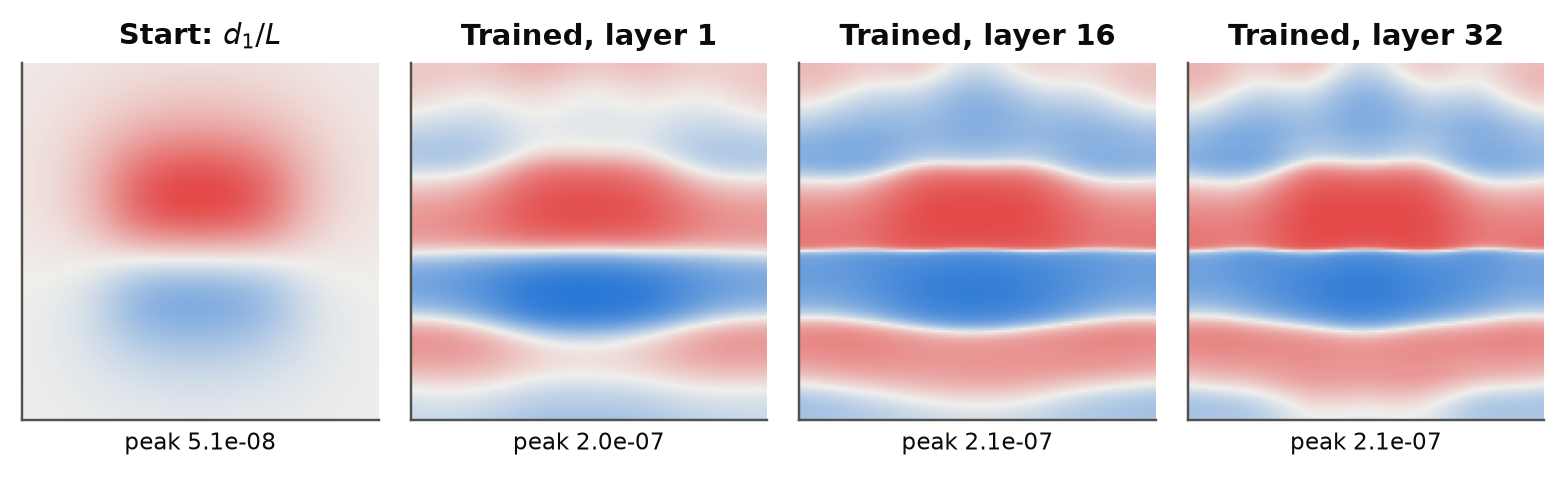
\includegraphics[width=\textwidth]{filters_w}
\caption{Filter $w_1$ for the first atom, at the start and after training, from the strict 32-layer
model at its best step. Each panel has its own colour scale. Training made the filters about four times
stronger, and added ripples.}
\label{fig:w}
\end{figure}

Figure~\ref{fig:w} shows something useful. The start is a smooth blob. After training, the filter has
alternating bands. Sign-changing ripples like that are what sharpening filters look like, since they
boost the frequencies that blur removed. For this atom, the trained filters also differ little between layers.

\chapter{Learning the dictionary}\label{ch:dictionary}

Before CSC-LISTA can train, it needs the atoms $g_m$. The paper's order is the same: learn a dictionary
first, then build the network on top of it, with the dictionary held fixed.

\section{The goal}

Find 32 small atoms, 75 pixels (7.5\um) wide, so that \emph{sharp} simulated fields can be written as
$\sum_m g_m*x_m$ with sparse $x_m$. This stage uses only sharp targets. It never sees the blurred input.

\section{The method: alternate two steps}

Neither the atoms nor the codes are known. So we hold one fixed and improve the other, again and again.

\begin{center}
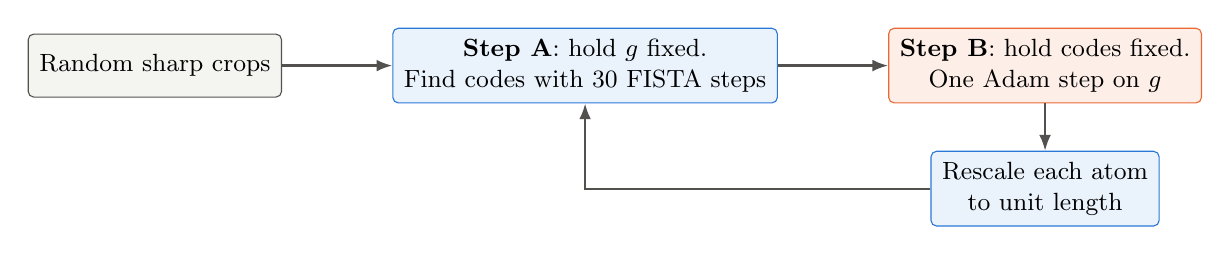
\begin{tikzpicture}[node distance=6mm and 14mm]
\node[fixed] (crop) {Random sharp crops};
\node[block,right=of crop] (code) {\textbf{Step A}: hold $g$ fixed.\\ Find codes with 30 FISTA steps};
\node[learned,right=of code] (update) {\textbf{Step B}: hold codes fixed.\\ One Adam step on $g$};
\node[block,below=of update] (norm) {Rescale each atom\\ to unit length};
\draw[flow] (crop)--(code); \draw[flow] (code)--(update); \draw[flow] (update)--(norm);
\draw[flow] (norm.west) -| (code.south);
\end{tikzpicture}
\end{center}

\begin{code*}{csc_lista.py}
    for step in range(steps):
        pieces = random_crops(fields, batch, crop, generator, .02).to(device)
        target = torch.nn.functional.pad(pieces, (pad, pad, pad, pad))
        with torch.no_grad():
            x = code_ista(target, Operator(g.data), lam, sparse_steps, pad)
        error = mask * (Operator(g).forward(x) - target)
        loss = .5 * (error ** 2).sum() / batch
        optimiser.zero_grad()
        loss.backward()
        optimiser.step()
        with torch.no_grad():
            g.copy_(unit_norm(g))
\end{code*}

\begin{itemize}
\item \code{code_ista} is FISTA with \code{g} held fixed, and \code{no_grad} means no gradients flow
through it. That is Step A.
\item The \code{error} and \code{loss} lines are Step B, one gradient step on the atoms.
\item \code{unit_norm} rescales each atom to length 1. Without it, atoms could grow and codes could
shrink, which would cheat the $\ell_1$ penalty.
\end{itemize}

The atoms start as real crops of training fields, with the mean removed. Settings: 600 steps, batch 8,
crops of 256 pixels.

\begin{careful}
This procedure is ours. The paper learns its dictionary with Algorithm 1 of Liu et al.\ 2018, which we did
not implement. Alternating sparse coding and gradient steps is a standard idea, but it is a substitute.
\end{careful}

\section{Choosing $\lambda$}

$\lambda$ sets the trade-off between accuracy and sparsity. An early pilot with small $\lambda$ gave codes
that were too dense, so a stronger set was tried. Each dictionary was scored on simulated validation crops,
using 200 FISTA steps.

\begin{center}
\begin{tabular}{ccc}
\toprule
$\lambda$ & Relative $L_2$ of the fit & Density of the codes \\
\midrule
0.1 & 3.2\% & 5.2\% \\
\textbf{0.3} & \textbf{6.4\%} & \textbf{2.4\%} \\
1.0 & 13.8\% & 1.0\% \\
\bottomrule
\end{tabular}
\end{center}

$\lambda=0.3$ was chosen by judgement, as a good balance. The code's automatic rule would have picked
the lowest error, $\lambda=0.1$, but this dictionary was passed in by hand with \code{--dictionary}.

\begin{keyidea}[Why this table is good news]
A fit error of 6.4\% with only 2.4\% of the code values active means 32 atoms really can describe
these fields sparsely. If this had failed, training a network on top would have been pointless.
\end{keyidea}

\section{What the atoms look like}

\begin{figure}[H]
\centering
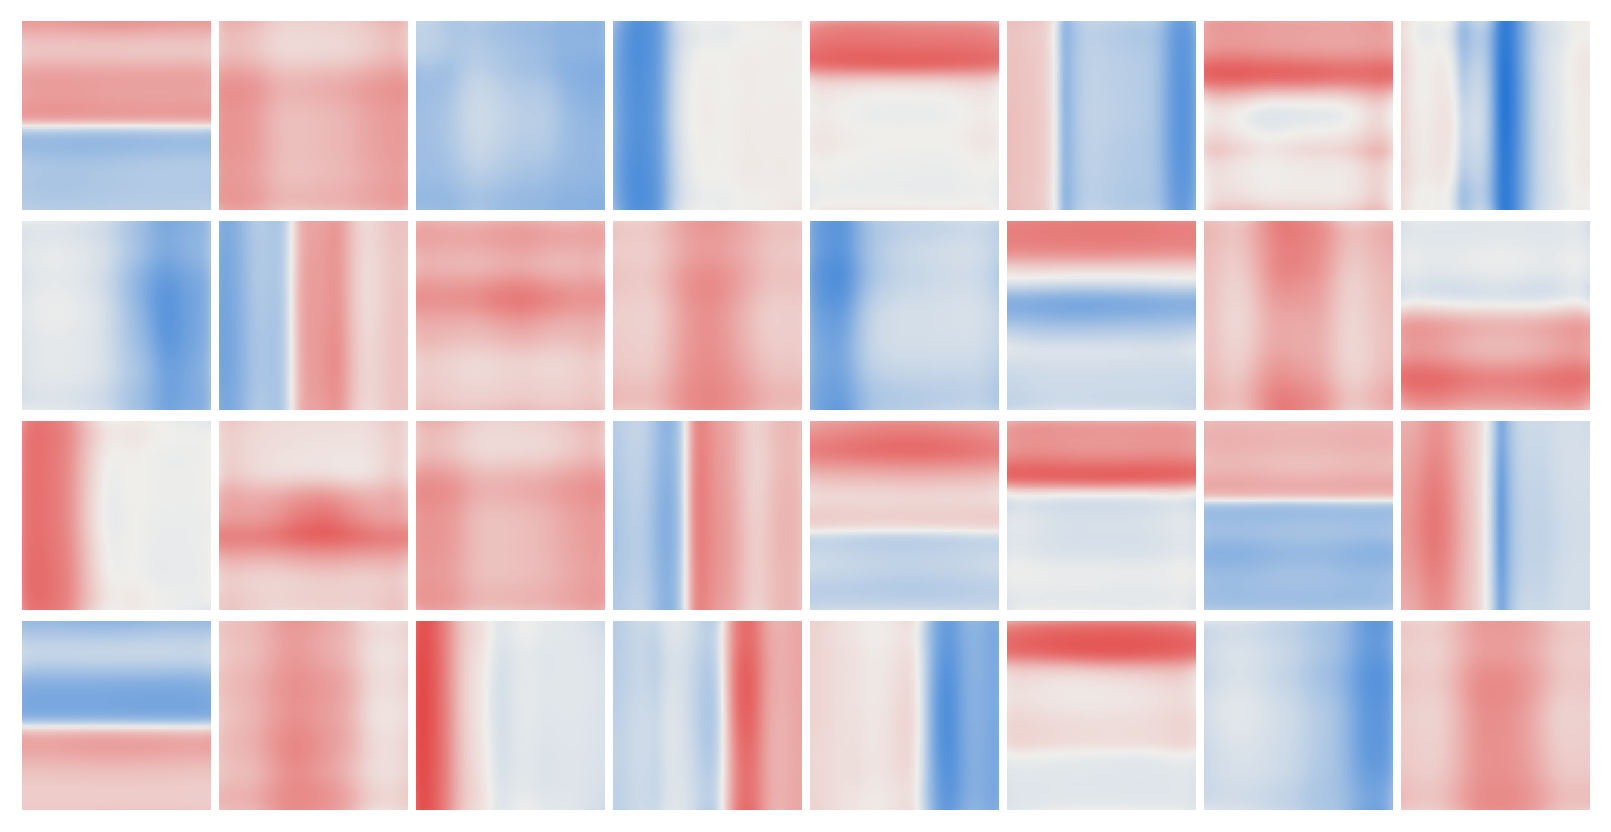
\includegraphics[width=\textwidth]{atoms}
\caption{All 32 learned atoms $g_m$, each 7.5\um\ wide. Red and blue are opposite signs.}
\label{fig:atoms}
\end{figure}

Most atoms in Figure~\ref{fig:atoms} are bars with a sign change. This makes physical sense. The field above
a straight wire has that shape, and our wires are straight segments. The dictionary rediscovered wires from the
data.

\begin{careful}
All three components share one dictionary, and it was trained on the simulated data, so it knows
about Manhattan wires of 1.6--3.2\um. A very different layout would need a new dictionary.
\end{careful}

\chapter{Training CSC-LISTA}\label{ch:training}

\section{One training step}

\begin{enumerate}
\item Pick 8 random 512 pixel crops of simulated fields. A crop must contain real signal: its peak
must be at least 0.05 in normalised units, or the code tries another position.
\item Pad each input to 768 pixels.
\item Run the network.
\item Compute the loss on the middle of the crop. A margin of 64 pixels is dropped on each side,
because edges are the least reliable.
\item Backpropagate, clip the gradient, take an Adam step.
\end{enumerate}

\begin{code*}{train_csc_lista.py}
            y = model(b)[..., pad:-pad, pad:-pad]
            keep = (slice(None), slice(margin, -margin), slice(margin, -margin))
            loss = crop_loss(y[keep], target[keep], args.loss)
        optimiser.zero_grad()
        loss.backward()
        torch.nn.utils.clip_grad_norm_(model.parameters(), 1.0)
        optimiser.step()
        schedule.step()
\end{code*}

\section{The loss: MSE or relative}

\begin{code*}{train_csc_lista.py}
def crop_loss(output, target, kind):
    """Mean squared error, or the mean per-crop relative L2 used for validation."""
    if kind == 'relative':
        return relative_l2(output, target).mean()
    return ((output - target) ** 2).mean()
\end{code*}

\textbf{MSE} is the paper's loss. It counts every pixel's squared error equally, so crops with strong fields
dominate. \textbf{Relative} divides by each crop's own size, so all crops count equally. It is also exactly the
metric we report. We tried it because of a problem you will see in Chapter~\ref{ch:density}.

\section{The learning rate problem}

The first attempt crashed with NaN. The filters start around $2\times10^{-8}$ in size, and a normal Adam
rate of $10^{-4}$ means each step is thousands of times larger than the value it changes. So the rate is now set
relative to each parameter's own scale.

\begin{code*}{train_csc_lista.py}
    # Filters start near 1e-8, so a fixed rate would swamp them; scale it to each.
    groups = [dict(params=[model.w], lr=args.lr_relative * float(model.w.pow(2).mean().sqrt())),
              dict(params=[model.theta], lr=args.lr_relative * float(model.theta.abs().mean()))]
\end{code*}

With \code{lr_relative} at 0.03, each step changes a parameter by about 3\% of the typical size. The rate then
decays along a cosine curve to zero by the last step.

\section{Validation and checkpoints}

Every 100 or 250 steps, the model is scored on 64 fixed crops from the validation layouts, which are
never trained on. If the score beats the best so far, the model is saved to \code{best.pt}. After training,
that best checkpoint is loaded and used for the COMSOL score.

\begin{code*}{train_csc_lista.py}
            if step == 0 or score < best:
                best = score
                torch.save(dict(state=model.state_dict(), step=step, score=score),
                           output / 'best.pt')
\end{code*}

This matters a lot. In the strict runs the best step came very early, at 300 of 1,000 and 200 of 1,000.

\begin{careful}[Validation and COMSOL scores cannot be compared directly]
Validation crops are chosen to contain signal, and COMSOL scores use the full image, including large
blank areas. So ``48.8\% on validation and 33.8\% on COMSOL'' does not mean COMSOL is easier.
\end{careful}

\section{Does the filter size matter?}

You asked whether to make $w$ bigger. The physics suggested it might, since the blurred kernel has a long
tail. Three 800-step trials on simulated validation gave a clear answer.

\begin{center}
\begin{tabular}{cc}
\toprule
Filter width & Validation error \\
\midrule
155 px & 52.35\% \\
255 px & 52.02\% \\
355 px & 51.99\% \\
\bottomrule
\end{tabular}
\end{center}

The difference is about a third of a point, and larger filters cost much more. So 155 stayed.

\section{Hardware}

All runs used the RTX A6000 with 48 GB, at batch 8.

\begin{center}
\begin{tabular}{rrrr}
\toprule
Layers & Parameters & Peak GPU memory & Time \\
\midrule
16 & 12.3 million & 12.8 GiB & 10,940 s for 2,000 steps \\
32 & 24.6 million & 22.0 GiB & 5,037 s for 1,000 steps \\
64 & 49.2 million & 40.2 GiB & 10,058 s for 1,000 steps \\
\bottomrule
\end{tabular}
\end{center}

Memory and time both grow with the number of layers, as you would expect from a chain of identical
layers. Also note the two lengths: the first runs took 2,000 steps. Once MSE was seen to peak early, later
runs used 1,000.

\begin{careful}[One seed]
Every run here used a single random seed. A difference of less than a point or so between two runs may
be luck. No error bars exist.
\end{careful}

\chapter{Density, plain, sparse and strict}\label{ch:density}

You said you did not understand this part. It is the most confusing part of the project, so we go
slowly. These are the four words to learn:

\begin{center}
\begin{tabularx}{\textwidth}{lX}
\toprule
Word & Meaning \\
\midrule
\textbf{Density} & The fraction of code values that are not exactly zero \\
\textbf{Plain} & Thresholds may fall as low as zero. Nothing stops them. Loss is MSE \\
\textbf{Sparse} & Thresholds are forbidden to fall below their starting value. Our addition \\
\textbf{Strict} & The same as plain, run at 32 and 64 layers, with nothing added \\
\bottomrule
\end{tabularx}
\end{center}

\section{What density is}

The network's final codes $x$ form a huge array: 32 maps of $768\times768$ values. Sparse coding promises
that almost all of them are zero. Density measures how true that is.

\begin{code*}{train_csc_lista.py}
                density = float((model.codes(sample) != 0).float().mean())
\end{code*}

So a density of 2\% means 98\% of the values are exactly zero. A density of 100\% means none are.
Our classical reference is the dictionary's own 2.4\%, from Chapter~\ref{ch:dictionary}.

\section{What went wrong}

The first full run had no restrictions: Eq.~20, MSE, 16 layers. It worked well, scoring 39.1\% on COMSOL. But
look at its density.

\begin{center}
\begin{tabular}{ll}
\toprule
Training step & Density \\
\midrule
0 (before training) & 20\% \\
250 & 99.9\% \\
\bottomrule
\end{tabular}
\end{center}

Within 250 steps, the code went from fairly sparse to completely full. The likely reason is simple.
Nothing in the MSE loss rewards sparsity. It only asks for a good output. Shrinking throws information
away, so training finds that the output improves when $\theta$ gets smaller. In the strict 32-layer
model, 6 of 32 thresholds hit exactly zero, and 19 others fell below the start. Only 7 rose.

\begin{figure}[H]
\centering
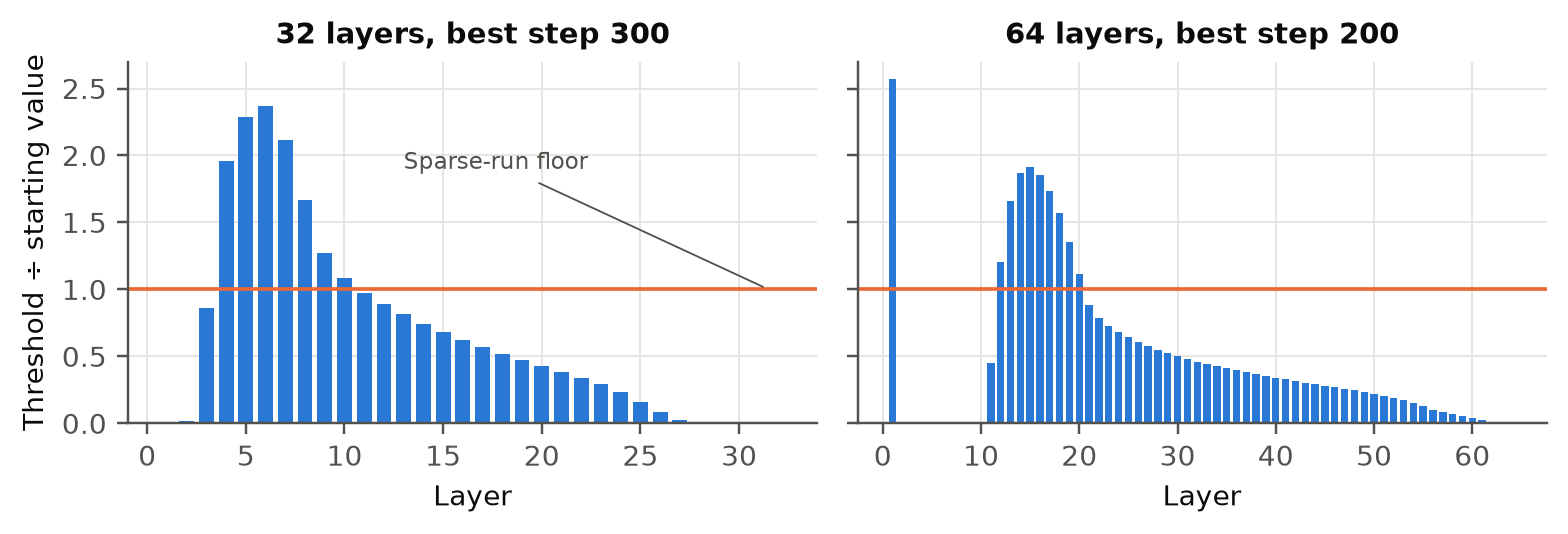
\includegraphics[width=\textwidth]{thresholds}
\caption{Learned threshold in each layer, divided by its starting value $\lambda/L$, for the two strict
models at their best step. The orange line at 1 is the lowest value allowed in sparse runs. No visible
bar means zero or nearly zero: the logs count 6 of 32 and 9 of 64 thresholds as exactly zero.}
\label{fig:thresholds}
\end{figure}

\begin{keyidea}[What a zero threshold means]
The logs print ``zero thresholds 6/32''. That counts layers with $\theta\le0$. With $\theta=0$, the shrink
function does nothing at all: $\soft_0(x)=x$. That layer is purely linear.
\end{keyidea}

\begin{careful}[The density number mostly reflects the last layer]
Density is measured on the final $x$, and the last step of the network is a shrink with $\theta^{(K)}$. If
that one threshold is zero, then almost no value is exactly zero, however the earlier layers behaved. In the
strict 32-layer model the last threshold is exactly 0, and density is about 100\%. In the strict 64-layer
model it is tiny but not zero, and density jumps around between 73\% and 99\% from checkpoint to checkpoint.
So treat this number as a coarse signal, not a precise measure.
\end{careful}

\section{So what is the network actually doing?}

At density near 100\%, with some thresholds at zero, there is little sparse coding left. The network acts
mostly as a \textbf{learned, nearly linear deconvolution}: a deep stack of filters. It starts as ISTA, and it uses
the ISTA structure as a good starting shape. But the final object is not finding a few active atoms.

\begin{defend}
\textbf{``Is this still sparse coding?''} Be honest: the structure is, the behaviour mostly is not. Do not
describe the strict models as sparse. The accurate sentence is: ``It is Eq.~20 of Liu et al., but
after MSE training the codes are dense, so it behaves like a learned deconvolution.''
\end{defend}

\section{Sparse runs: an attempt to fix it}

To force sparsity, I added one option that keeps thresholds at or above a floor.

\begin{code*}{train_csc_lista.py}
    floor = args.theta_floor * float(model.theta.min())
\end{code*}
\begin{code*}{train_csc_lista.py}
        with torch.no_grad():
            model.theta.clamp_(min=floor)
\end{code*}

This single flag is the difference between the names:

\begin{itemize}
\item \code{--theta-floor 0}: thresholds can reach zero. This is \textbf{plain}.
\item \code{--theta-floor 1}: thresholds stay at or above $\lambda/L$. This is \textbf{sparse}.
\end{itemize}

\textbf{There is no separate ``sparse Eq.~20'' in the paper.} Both are the same equation. Sparse is Eq.~20 plus my
constraint on one parameter. The result:

\begin{center}
\begin{tabular}{lcccc}
\toprule
16 layers, MSE & Density at best step & Simulated validation & COMSOL \\
\midrule
Plain & 99.9\% & 53.4\% & 39.1\% \\
Sparse & 28.8\% & 48.6\% & 40.2\% \\
\bottomrule
\end{tabular}
\end{center}

The floor worked in one sense: density fell to about 29\%, still far above the dictionary's 2.4\%. And it
helped on simulation. But it made COMSOL slightly \emph{worse}.

\section{Relative loss: a second attempt}

The MSE curves peaked at step 250 and then got worse, even though training continued. That pointed to a
mismatch between the loss and the metric. So the next runs used the relative loss, and added more layers.

\section{Every CSC-LISTA run in one table}

\begin{center}
\small
\begin{tabular}{lrrlcrrrr}
\toprule
Name & Layers & Steps & Loss & Floor & Best step & Density & Simulated & COMSOL \\
\midrule
Plain & 16 & 2,000 & MSE & no & 250 & 99.9\% & 53.4\% & 39.1\% \\
Sparse MSE & 16 & 2,000 & MSE & yes & 250 & 28.8\% & 48.6\% & 40.2\% \\
Sparse relative & 16 & 1,000 & Relative & yes & 1,000 & 25.6\% & 45.6\% & 42.0\% \\
Sparse relative & 32 & 1,000 & Relative & yes & 700 & 22.1\% & 42.5\% & 38.9\% \\
\textbf{Strict} & \textbf{32} & \textbf{1,000} & \textbf{MSE} & \textbf{no} & \textbf{300} & \textbf{99.9\%} & \textbf{51.9\%} & \textbf{35.4\%} \\
\textbf{Strict} & \textbf{64} & \textbf{1,000} & \textbf{MSE} & \textbf{no} & \textbf{200} & \textbf{74.2\%} & \textbf{48.8\%} & \textbf{33.8\%} \\
\bottomrule
\end{tabular}
\end{center}

Density is the value logged at the best step. Plain and strict have the same settings, apart from the number of
layers, the length of the run, and how often validation ran: every 250 steps for plain and every 100 for strict. The
Eq.~20 layer is identical in both code versions.

\begin{figure}[H]
\centering
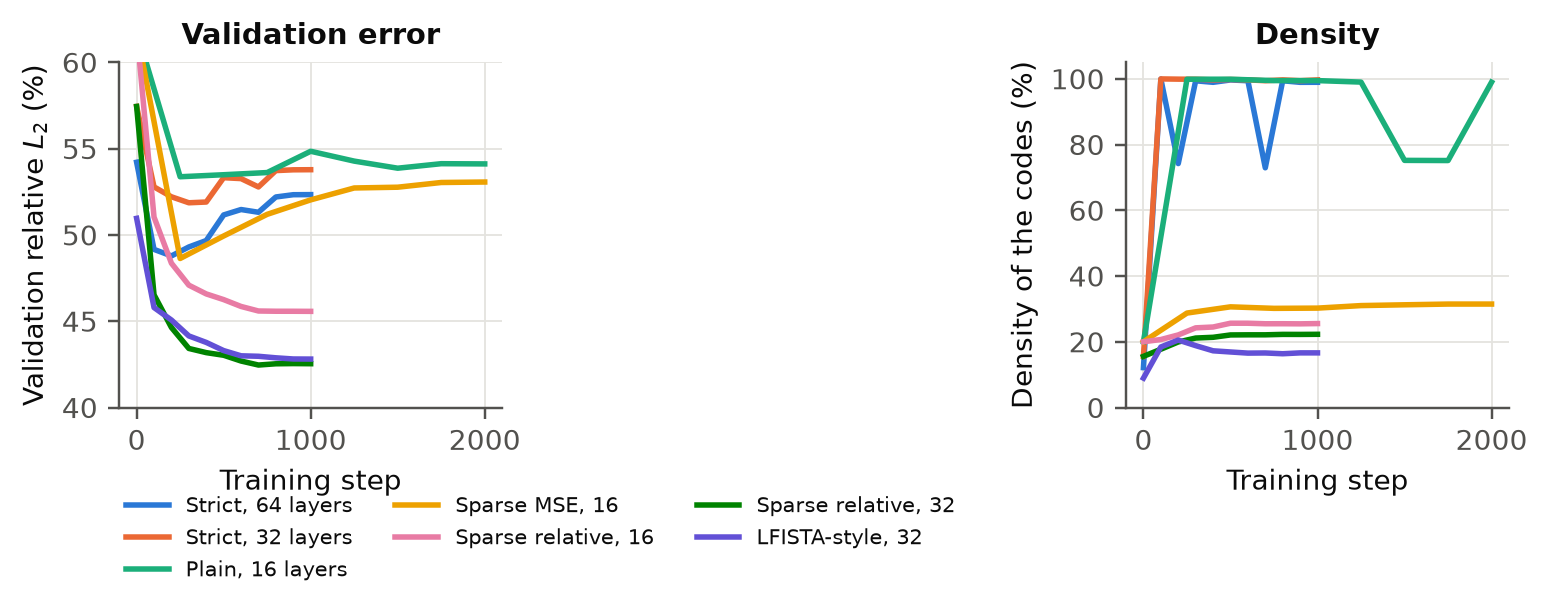
\includegraphics[width=\textwidth]{curves}
\caption{Validation error and density during training. Plain and strict runs jump to near 100\% density almost
at once. Sparse runs stay low. MSE runs reach their best validation error early, then get worse.}
\label{fig:curves}
\end{figure}

\section{Why ``strict'' exists}

After the sparse runs you asked whether everything was exactly what the paper did, because you cannot
defend additions. The honest answer was no. So we removed the floor and the relative loss, and reran
Eq.~20 as closely as we could at 32 and 64 layers. You also asked why rerun 32 layers when it had already
run. The earlier 32-layer run had the floor and the relative loss, so it was not strict.

And here is the surprise.

\begin{keyidea}[The result you should remember]
Removing my additions made the COMSOL score better: 38.9\% became 35.4\% at the same 32 layers. The sparse
version looked far better on simulated validation, but lost on COMSOL. Simpler was better, and it is
also more defensible.
\end{keyidea}

\section{What the later runs add to this story}

Two later results change how to think about density.

\textbf{Dense codes are not required.} The LFISTA-style network of Chapter~\ref{ch:lfista} is trained on the Lasso objective,
which includes the $\ell_1$ penalty, so its loss does reward sparsity. Its density stayed at 16.6\%, none of its 32
thresholds reached zero, and it still scored 34.2\%, close to strict 64 layers. This suggests the loss decides it: MSE lets
the codes fill up, and Lasso keeps them sparse. That is one run of each, so treat it as a strong hint.

\textbf{Our best method is not very sparse either.} On the crop in Figure~\ref{fig:reconstruction}, FISTA-300 with
$\lambda=0.009$ has a density of 27.6\%. The dictionary's 2.4\% came from fitting sharp fields with $\lambda=0.3$, which is a
different problem. So 2.4\% is not a fair target for deblurring.

\chapter{Results}\label{ch:results}

All server runs have finished. FISTA has been rescored at matching depths, and FISTA-Net has been rerun.

\section{The main table}

All numbers are mean errors. Lower is better.

\begin{center}
\small
\begin{tabular}{lccc}
\toprule
Method & Simulated validation & COMSOL (15 pairs) & COMSOL NRMSE \\
\midrule
ISTA, 16 iterations & 64.3\% & 64.4\% & 4.60\% \\
Wiener & 60.3\% & 49.3\% & 3.53\% \\
Eq.~20, sparse, relative, 16 layers & 45.6\% & 42.0\% & 3.01\% \\
FISTA-32, $\lambda=0.03$ & 50.9\% & 41.8\% & 3.00\% \\
Eq.~20, sparse, MSE, 16 layers & 48.6\% & 40.2\% & 2.88\% \\
FISTA-Net run 1 & 65.2\% & 39.4\% & 2.85\% \\
Eq.~20, plain, MSE, 16 layers & 53.4\% & 39.1\% & 2.80\% \\
Eq.~20, sparse, relative, 32 layers & 42.5\% & 38.9\% & 2.80\% \\
FISTA-64, $\lambda=0.009$ & 45.3\% & 37.9\% & 2.72\% \\
Eq.~20, strict, 32 layers & 51.9\% & 35.4\% & 2.54\% \\
LFISTA-style, 32 layers & 42.8\% & 34.2\% & 2.47\% \\
Eq.~20, strict, 64 layers & 48.8\% & 33.8\% & 2.43\% \\
\textbf{FISTA-Net run 2} & \textbf{47.9\%} & \textbf{33.3\%} & \textbf{2.41\%} \\
FISTA-300, $\lambda=0.03$ & 36.6\% & 32.1\% & 2.33\% \\
\textbf{FISTA-300, $\lambda=0.009$} & \textbf{35.5\%} & \textbf{30.5\%} & \textbf{2.20\%} \\
\bottomrule
\end{tabular}
\end{center}

\begin{figure}[H]
\centering
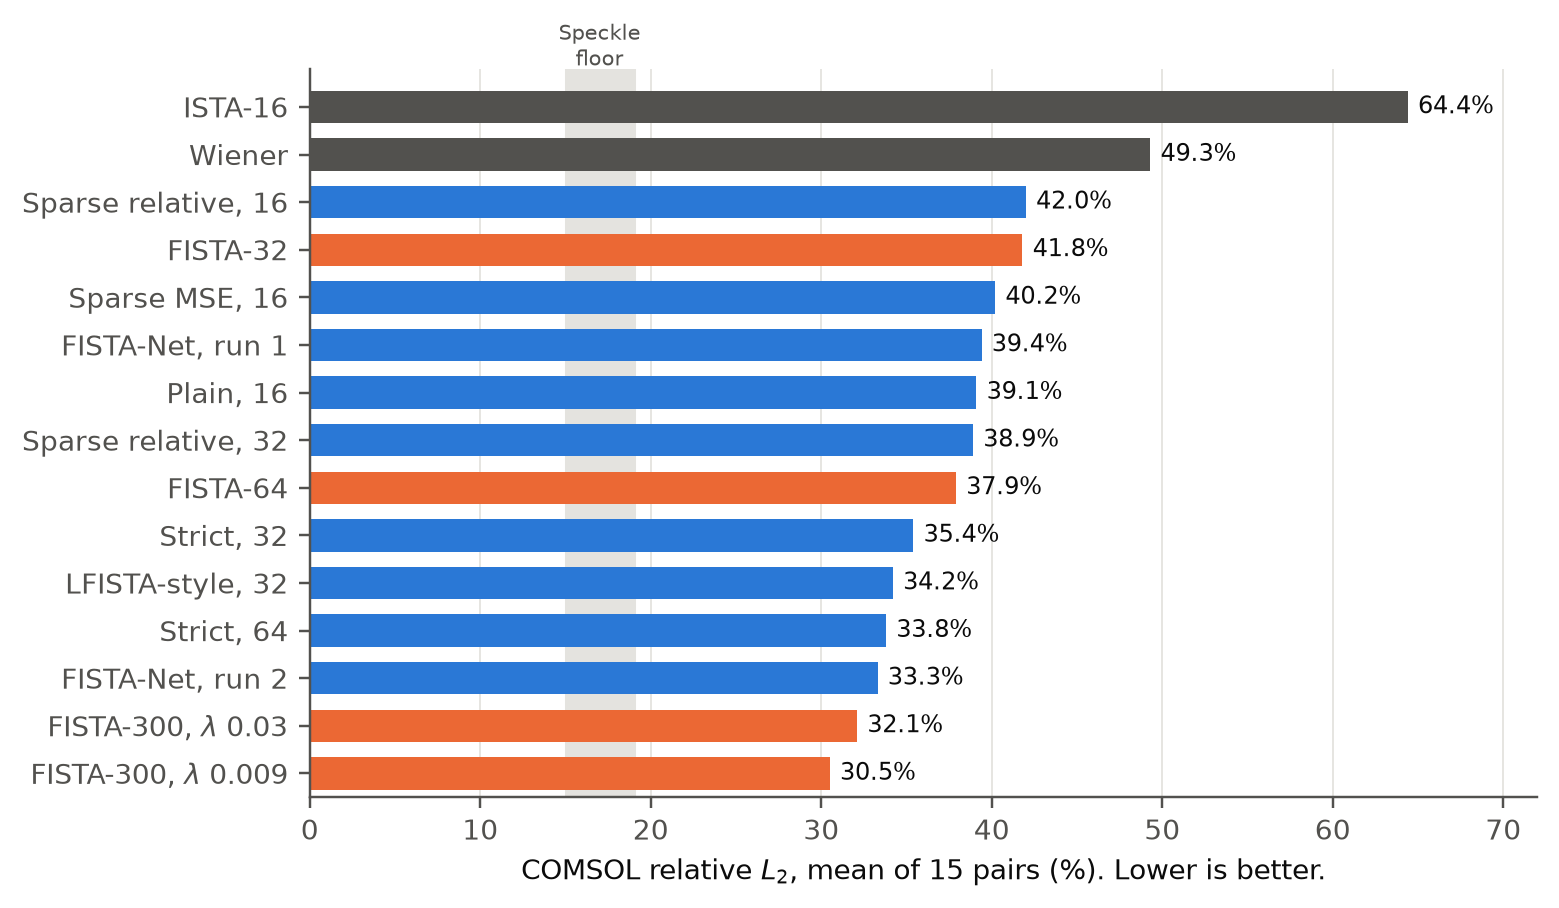
\includegraphics[width=\textwidth]{results}
\caption{The COMSOL scores from the table. Grey bars are simple baselines, blue bars are trained networks, and
orange bars are FISTA with the same dictionary and no trained layers. The shaded band is the speckle floor
from Chapter~\ref{ch:simulation}.}
\label{fig:results}
\end{figure}

\begin{keyidea}[The current picture]
\begin{itemize}
\item \textbf{Best overall:} FISTA-300 at 30.5\%, a classical method using the learned dictionary.
\item \textbf{Selected network:} FISTA-Net run 2, 33.3\%. Among the runs without our floor and loss changes, it has the
lowest simulated validation error, so this choice does not use COMSOL.
\item \textbf{Close behind:} strict Eq.~20 at 64 layers, 33.8\%, and the LFISTA-style network, 34.2\%. All three networks sit
within 1 point, which is too small to rank on one seed each.
\end{itemize}
\end{keyidea}

\section{Networks against FISTA at equal depth}

This is the fair way to ask whether learning helped. One layer and one FISTA iteration do similar work, so
compare them at the same count.

\begin{center}
\begin{tabular}{rcccc}
\toprule
& \multicolumn{2}{c}{COMSOL} & \multicolumn{2}{c}{Simulated validation} \\
Depth & FISTA & Strict Eq.~20 & FISTA & Strict Eq.~20 \\
\midrule
32 & 41.8\% & \textbf{35.4\%} & \textbf{50.9\%} & 51.9\% \\
64 & 37.9\% & \textbf{33.8\%} & 45.3\% & 48.8\% \\
300 & 30.5\% & Not trained & 35.5\% & Not trained \\
\bottomrule
\end{tabular}
\end{center}

\begin{figure}[H]
\centering
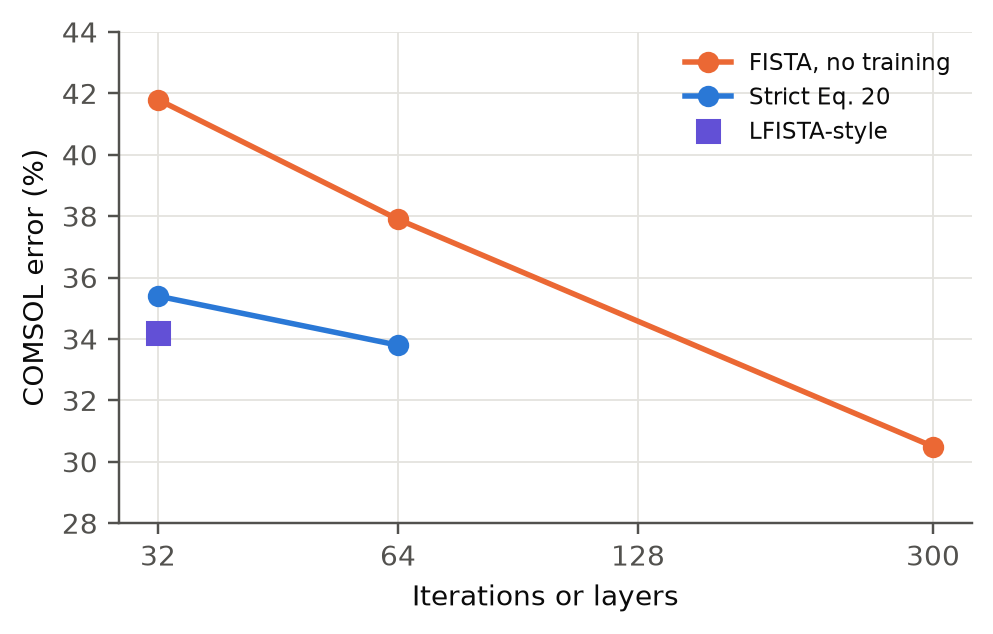
\includegraphics[width=.68\textwidth]{depth}
\caption{COMSOL error against depth. At 32 and 64 steps the networks win. FISTA keeps improving with more
iterations and passes them by 300. Note the log scale.}
\label{fig:depth}
\end{figure}

So on COMSOL, learning gives a gain of about 6 points at 32 layers and 4 at 64. On simulated validation, the same
networks \emph{lose} to FISTA at the same depth, by 1 and 3.5 points. The gain appears only on COMSOL, and we do not
know why. It is worth being careful about this before claiming it as a win.

\begin{careful}[No speed claim yet]
It is tempting to say that 64 layers do the work of about 300 iterations, but that is not what the data shows, since
64 layers do not reach FISTA-300's score. Also, run time was never measured. So there is no speed advantage you can claim
yet.
\end{careful}

\section{How FISTA's $\lambda$ was retuned}

The first version of this booklet warned that $\lambda=0.03$ sat at the edge of the search grid. So FISTA was rescored per
depth with \code{scripts/score_fista_depths.py}, on a wider grid. Each $\lambda$ was again chosen on the first 16
simulated validation crops only.

\begin{center}
\begin{tabular}{ccccccccc}
\toprule
$\lambda$ & 7e-7 & 0.0003 & 0.003 & 0.009 & 0.03 & 0.09 & 0.3 & 0.9 \\
\midrule
FISTA-300 on 16 crops & 40.0\% & 36.1\% & 24.4\% & \textbf{22.4\%} & 24.5\% & 29.4\% & 41.3\% & 55.3\% \\
\bottomrule
\end{tabular}
\end{center}

Now the best value sits inside the grid, with worse values on both sides. The chosen values are 0.03 for FISTA-32 and
0.009 for FISTA-64 and FISTA-300. The old $\lambda=0.03$ score reproduced exactly, at 32.1\%, which confirms that the new
script and the first run agree.

\begin{careful}[FISTA-64's $\lambda$ is uncertain]
The 16 crops chose 0.009, but on all 64 crops 0.03 was slightly better, 44.9\% against 45.3\%. Both give about 38\% on
COMSOL, so it barely matters here, but 16 crops is a small sample.
\end{careful}

\section{By component and configuration}

\begin{center}
\begin{tabular}{lccc}
\toprule
Mean over 5 configurations & $B_x$ & $B_y$ & $B_z$ \\
\midrule
Wiener & 47.7\% & 48.1\% & 52.2\% \\
FISTA-32 & 40.0\% & 40.2\% & 45.2\% \\
FISTA-Net run 1 & 36.2\% & 36.2\% & 46.0\% \\
FISTA-64, $\lambda=0.009$ & 36.2\% & 36.4\% & 41.2\% \\
Strict, 32 layers & 33.6\% & 33.6\% & 39.1\% \\
LFISTA-style, 32 layers & 32.8\% & 31.4\% & 38.5\% \\
FISTA-Net run 2 & 30.2\% & 30.7\% & 39.1\% \\
Strict, 64 layers & 31.8\% & 32.0\% & 37.5\% \\
FISTA-300, $\lambda=0.009$ & 29.0\% & 27.8\% & 34.7\% \\
\bottomrule
\end{tabular}
\end{center}

$B_z$ is always the hardest. This matches the simulator, which also has its largest error on $B_z$, and the speckle,
which is strongest there.

\begin{center}
\begin{tabular}{lccccc}
\toprule
Mean over 3 components & L1\_C1 & IC\_4um & C1+C2 & C1+C2+C3 & C1--C4 \\
\midrule
Wiener & 49.3\% & 50.1\% & 49.1\% & 49.0\% & 49.0\% \\
FISTA-32 & 41.2\% & 45.0\% & 41.0\% & 40.9\% & 41.0\% \\
FISTA-Net run 1 & 39.0\% & 42.1\% & 38.9\% & 38.7\% & 38.5\% \\
FISTA-Net run 2 & 33.1\% & 34.6\% & 33.2\% & 33.1\% & 32.7\% \\
FISTA-64, $\lambda=0.009$ & 38.3\% & 36.9\% & 38.2\% & 38.1\% & 38.1\% \\
Strict, 32 layers & 36.3\% & 32.3\% & 36.3\% & 36.1\% & 36.1\% \\
LFISTA-style, 32 layers & 35.3\% & 30.1\% & 35.3\% & 35.2\% & 35.2\% \\
Strict, 64 layers & 34.6\% & 30.7\% & 34.6\% & 34.5\% & 34.5\% \\
FISTA-300, $\lambda=0.009$ & 31.2\% & 27.6\% & 31.4\% & 31.2\% & 31.1\% \\
\bottomrule
\end{tabular}
\end{center}

Four of the five columns are nearly equal, because they contain the same wire shape. Only IC\_4um is a different coil. Most
methods do better on it, but FISTA-32 and both FISTA-Net runs do worse. So one extra wire shape can change the ranking, which is
another reason to treat 15 pairs from two shapes with care.

\section{What the outputs look like}

\begin{figure}[H]
\centering
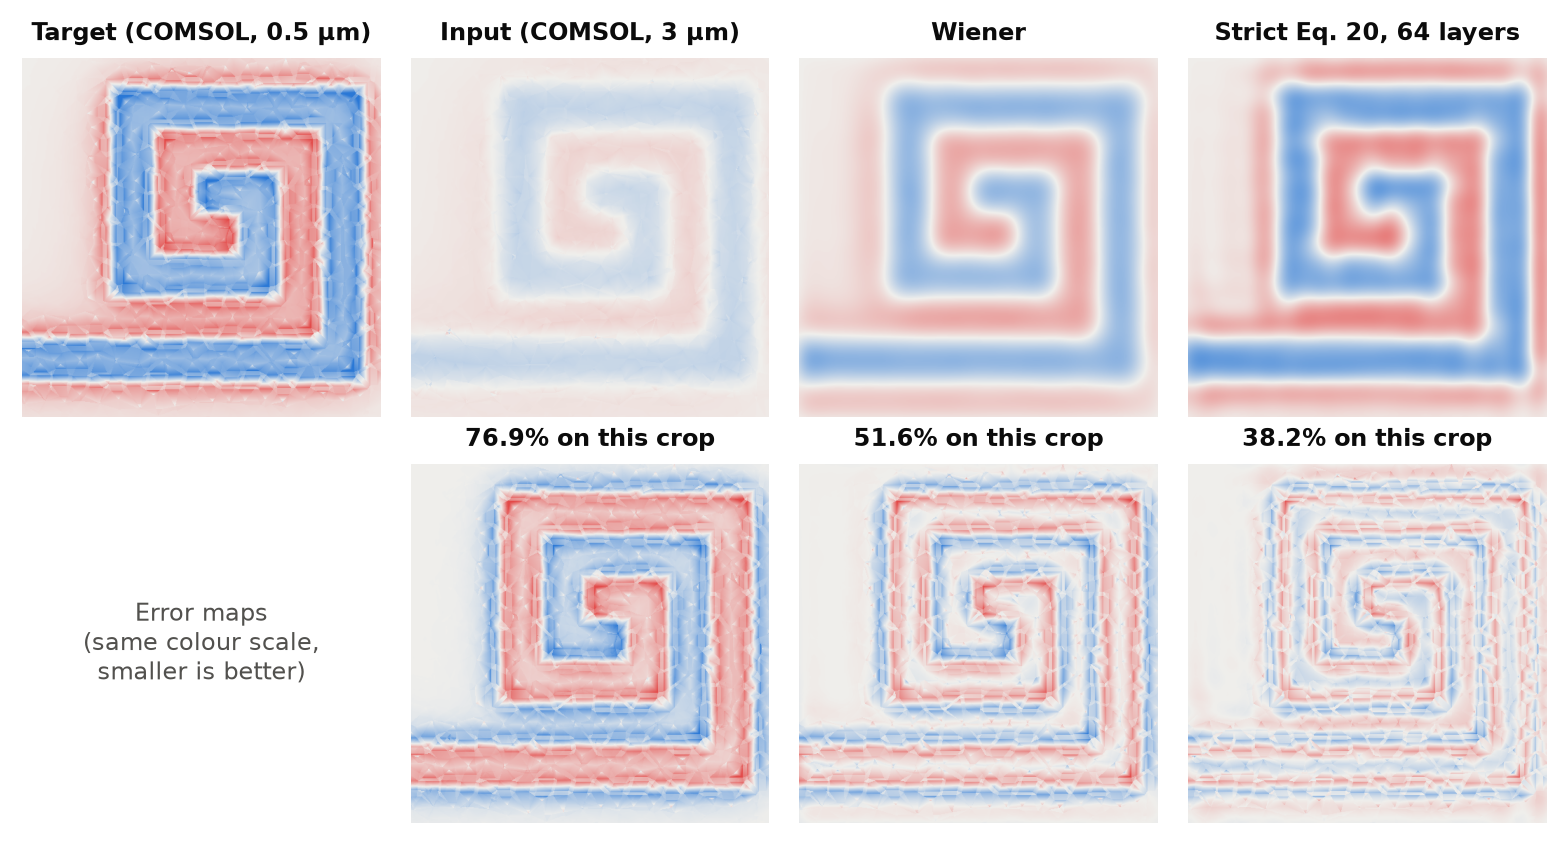
\includegraphics[width=\textwidth]{reconstruction}
\caption{$B_z$ of the COMSOL L1\_C1 coil, on the 512 pixel window with the most signal. The top row shares one colour
scale. The bottom row shows output minus target on that same scale. The output was computed from the zero-padded 512
pixel crop alone, so it is not a cut-out of the full-image prediction, and the percentages apply to this crop only.
Note the fine mesh speckle in the target: no method can or should reproduce it.}
\label{fig:reconstruction}
\end{figure}

Three things are visible in Figure~\ref{fig:reconstruction}.

\begin{enumerate}
\item The input is much too weak, so its error map still looks like the coil.
\item Wiener restores some strength, but its edges stay soft.
\item Strict Eq.~20 is much closer in strength, and its remaining error sits mostly on wire edges.
\end{enumerate}

\begin{figure}[H]
\centering
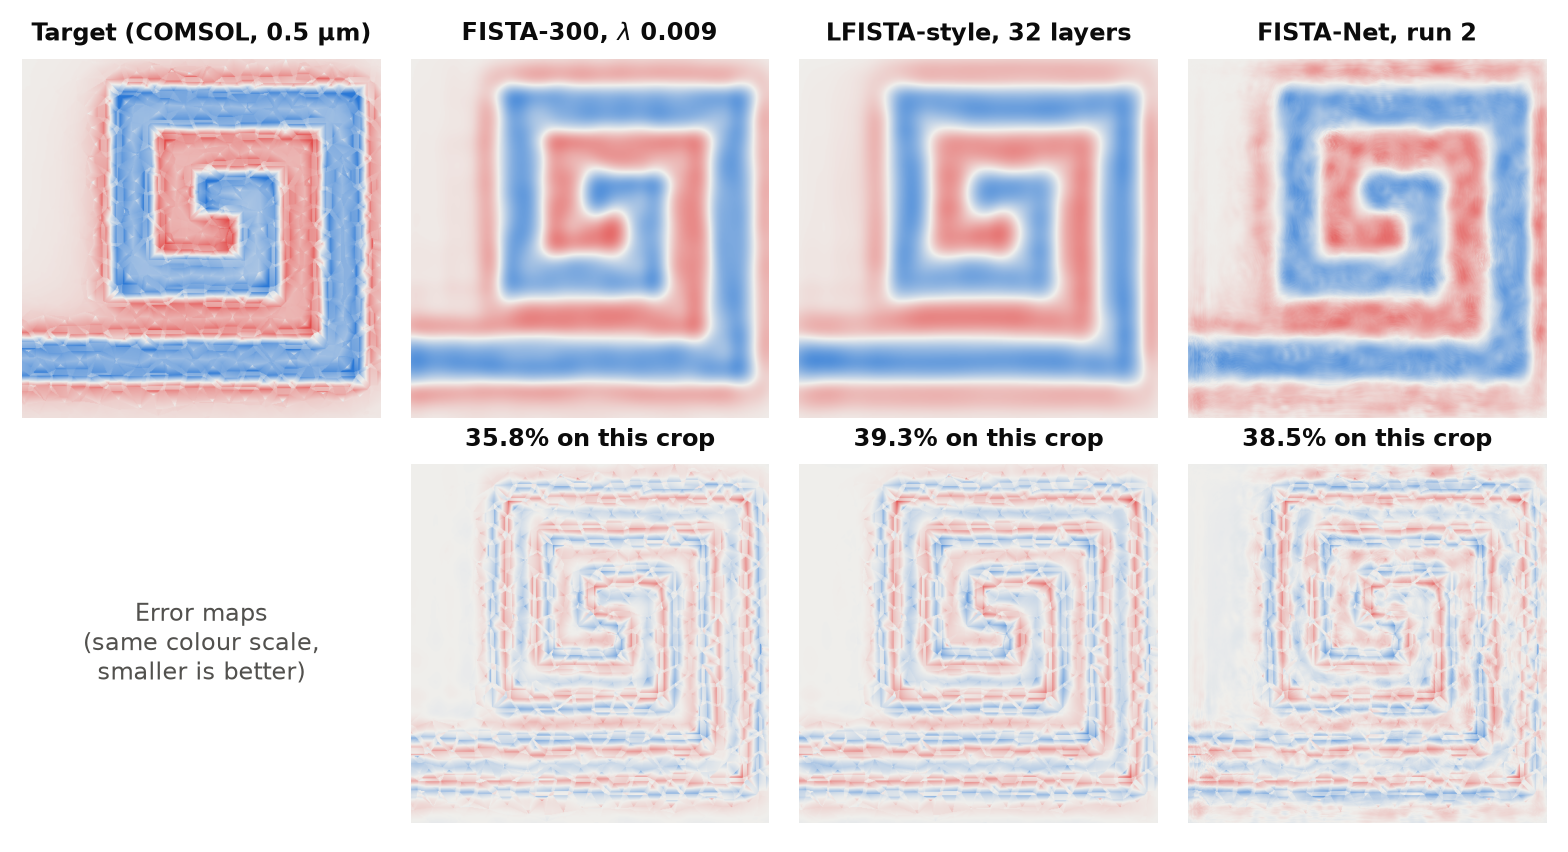
\includegraphics[width=\textwidth]{reconstruction_new}
\caption{The same crop and colour scale for three other methods. Again, the percentages apply to this crop only.}
\label{fig:reconstruction-new}
\end{figure}

\section{Seven honest lessons}

\subsection*{1. Depth helps every method}

Networks: 39.1, 35.4 and 33.8\% at 16, 32 and 64 layers. FISTA: 41.8, 37.9 and 30.5\% at 32, 64 and 300. For the networks,
the gain per doubling is shrinking, and the first of those runs also had a different length.

\subsection*{2. Learning helps at equal depth, but FISTA-300 still wins}

Strict Eq.~20 and the LFISTA-style network beat FISTA at 32 and 64 steps on COMSOL. Nothing trained so far reaches FISTA-300.

\subsection*{3. Simulated validation does not predict COMSOL}

\begin{figure}[H]
\centering
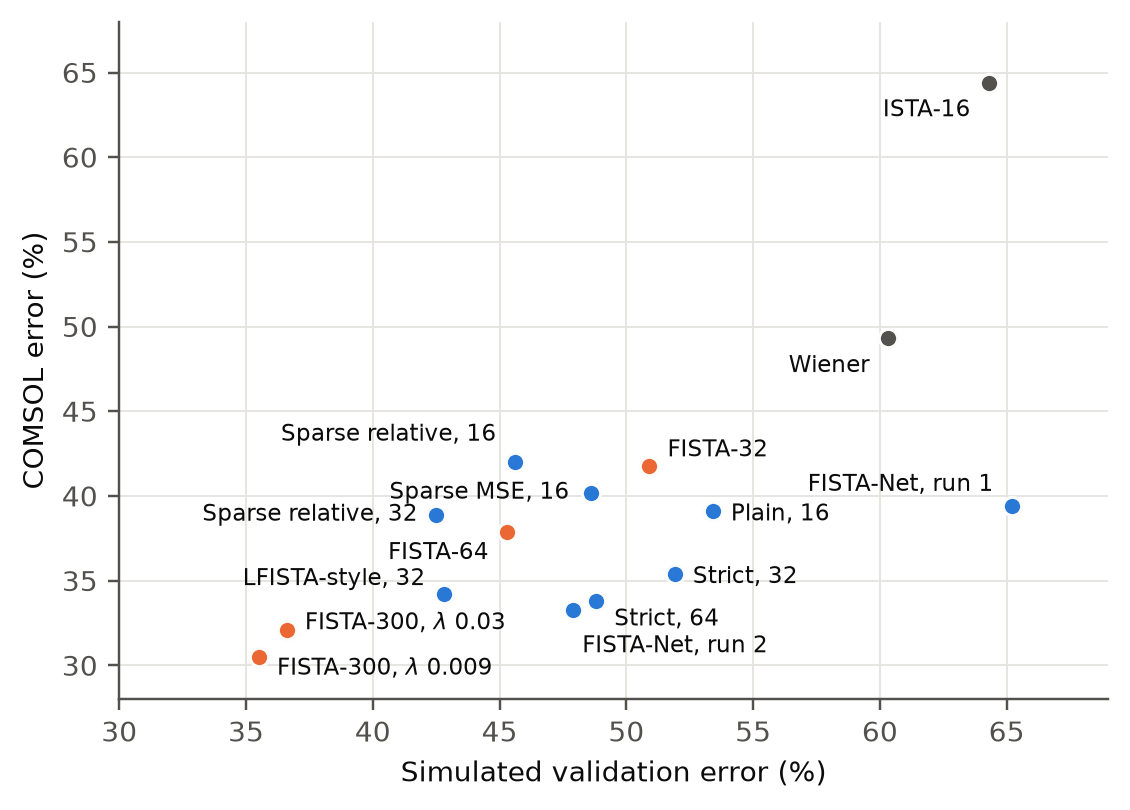
\includegraphics[width=.8\textwidth]{rank}
\caption{Each dot is a method. If simulated validation predicted COMSOL well, the dots would form a tight rising line.
FISTA-Net run 1 is the clearest exception: it has the worst simulated score of all, yet it beats Wiener, ISTA-16 and
FISTA-32 on COMSOL. The sparse 32-layer run also beats the two strict runs on simulation and loses to them on COMSOL.}
\label{fig:rank}
\end{figure}

This is the most important warning in this booklet. We pick checkpoints and settings on simulated validation, because
COMSOL must stay untouched. Yet Figure~\ref{fig:rank} shows that a better simulated score does not reliably give a better
COMSOL score. The simulator is not a perfect copy of COMSOL.

\subsection*{4. Early peaking belongs to the MSE runs}

MSE runs get their best validation score at step 200--300, then get worse. Strict 64 went from 48.8\% at step 200 to 52.3\%
at step 1,000. The LFISTA-style run behaves differently: its validation error improved all the way to the last step. It has
no target in its loss, so it cannot fit the training targets. This is a hint that MSE fitting is part of the problem, but it
is one run of each, and the cause is not established.

\subsection*{5. A sparse network can match a dense one}

The LFISTA-style network keeps its codes 16.6\% dense, and still reaches 34.2\%. So the dense behaviour of strict
Eq.~20 is not required for a good score. See Chapter~\ref{ch:density}.

\subsection*{6. A tiny network can match a huge one}

FISTA-Net has 74,599 parameters, and strict Eq.~20 at 64 layers has 49.2 million, about 660 times more. It also needs no
dictionary. Yet they score about the same. The price was training time: run 2 took about 27 hours, against about 3 for
strict 64 layers.

\subsection*{7. There is a floor}

COMSOL's speckle lies in the target, so no clean method should score below about 15--19\%. From FISTA-300's 30.5\%, that
leaves at most about 12--16 points.

\section{Caveats to state out loud}

\begin{careful}
\begin{itemize}
\item \textbf{Best of many.} After many methods are compared on COMSOL, the best score is a little optimistic, even though
no setting was chosen on COMSOL. If you keep trying methods and report only the winner, you are slowly using the test set.
\item \textbf{FISTA-Net got a second chance.} Run 2 exists because of what run 1 showed, and an interim COMSOL score was read
during run 2. It changed nothing in the run, but no other network was rerun this way.
\item \textbf{A noisy checkpoint.} FISTA-Net's validation error still swings widely, and its best step was picked from 91
checks, so 47.9\% is partly a lucky draw. Its last 300 steps ranged from 47.9\% to 54.3\%.
\item \textbf{The baseline moved.} FISTA was retuned after the COMSOL scores of the networks were known. The $\lambda$ was chosen on
simulated crops only, and the widening was prompted by the grid edge, not by a COMSOL score. Say this openly anyway.
\item \textbf{Unequal tuning.} FISTA got a search over eight $\lambda$ values. The LFISTA-style run still uses
$\lambda=0.03$, and $0.009$ has not been tried for it.
\item \textbf{Two wire shapes.} The 15 pairs are not 15 independent tests.
\item \textbf{One seed.} No error bars exist.
\item \textbf{Prior knowledge.} The generator was designed with these coils in view.
\end{itemize}
\end{careful}

\chapter{Paper versus code: every difference}\label{ch:differences}

This chapter is the one to bring to a meeting. It compares strict CSC-LISTA against Eq.~20 and Appendix H
of Liu et al. It is more complete than the table in \code{README_CSC_LISTA.md}.

\section{What matches the paper}

\begin{center}
\renewcommand{\arraystretch}{1.3}
\begin{tabularx}{\textwidth}{lX}
\toprule
Item & Status \\
\midrule
Layer update & Eq.~20, term by term. See Chapter~\ref{ch:csc_lista} \\
Filter per layer & $w^{(k)}$ learned separately per layer \\
Threshold & One $\theta^{(k)}$ per layer, shared by all atoms \\
Output & Codes convolved with the original dictionary, as in Appendix H \\
Loss & MSE between output and clean image, as in Appendix H \\
Order of work & Dictionary first, then the network with the dictionary fixed \\
\bottomrule
\end{tabularx}
\end{center}

\section{What is necessary for our problem}

\begin{center}
\renewcommand{\arraystretch}{1.3}
\begin{tabularx}{\textwidth}{>{\raggedright\arraybackslash}p{3.1cm}>{\raggedright\arraybackslash}X>{\raggedright\arraybackslash}X}
\toprule
Item & Paper & Ours, and why \\
\midrule
Task & Denoising, $b=t+$noise & Deblurring, $b=h*t+$noise. This is our problem \\
Dictionary in the data term & Small learned $d_m$, used directly & $d_m=h*g_m$, long blurred filters. This is how the blur gets into Eq.~20. No published result covers this use \\
Normalisation & $\lVert d_m\rVert_2=1$ & $\lVert g_m\rVert_2=1$, so the blurred $d_m$ are not unit length \\
Data & 400 natural images & Simulated fields, 512 pixel crops \\
Boundary & Non-circular, $x$ larger than $b$ (Eq.~18) & FFT with zero padding, codes on the padded canvas, and a window mask on the residual. Same purpose, different method \\
Layers & 5 & 16, 32 and 64, because the blur is far harder than the denoising task \\
\bottomrule
\end{tabularx}
\end{center}

\section{What is our own engineering choice}

\begin{center}
\renewcommand{\arraystretch}{1.3}
\begin{tabularx}{\textwidth}{>{\raggedright\arraybackslash}p{3.1cm}>{\raggedright\arraybackslash}X>{\raggedright\arraybackslash}X}
\toprule
Item & Paper & Ours \\
\midrule
Size of $w$ & Same size as $d_m$ & 155 pixels, shorter than the long blurred $d_m$. Trials showed little gain from larger \\
Dictionary learning & Algorithm 1 of Liu et al.\ 2018 & Alternating FISTA and Adam \\
Atoms & $M=64$, $D=7$ in its experiments & 32 atoms of 75 pixels \\
Start of $w$ & Not specified for Eq.~20 & ISTA values, $d_m/L$, truncated \\
Start of $\theta$ & Not specified for Eq.~20 & $\lambda/L$, with $\lambda=0.3$ \\
Optimiser & Not specified in Appendix H & Adam, with a rate 3\% of each parameter's scale \\
Rate schedule & Not specified & Cosine decay to zero \\
Gradient clipping & Not mentioned & Norm limited to 1.0 \\
Threshold sign & $\theta$ is a threshold, so $\ge0$ & \code{clamp_min(0)} in the layer, and a clamp at 0 after each step \\
Loss region & Not stated & Middle of the crop, 64 pixel margin dropped \\
Checkpoint & Not stated & Best simulated validation score \\
\bottomrule
\end{tabularx}
\end{center}

\section{Additions that strict runs removed}

\begin{center}
\renewcommand{\arraystretch}{1.3}
\begin{tabularx}{\textwidth}{lXl}
\toprule
Item & What it did & Used in \\
\midrule
Threshold floor & Kept $\theta$ at or above $\lambda/L$ & Sparse runs only \\
Relative loss & Replaced MSE with per-crop relative $L_2$ & Relative runs only \\
\bottomrule
\end{tabularx}
\end{center}

\begin{defend}[The short version to memorise]
``The layer, output and loss are from Eq.~20 and Appendix H of Liu et al. Three things are necessarily
ours. We deblur rather than denoise, so the dictionary is $h*g$. We use FFT convolution with padding
and a mask. And our dictionary learning is a substitute for theirs. Everything else is standard training
practice, listed in full.''
\end{defend}

\begin{careful}
A note on the paper's own text. Section 5 says the dictionary came from Algorithm 1 of Liu et al.\ 2018, while
Appendix H says it was obtained ``by solving (24)'', which is the analytic weight problem. The second looks
like loose wording, but the two statements do not match. If you are asked, quote Section 5.
\end{careful}

\section{Which code actually ran}

Each server run used a frozen copy of the scripts, so later edits could not change it. The local \code{scripts/} folder,
which this booklet quotes, is byte-identical to the frozen copy for FISTA-Net run 2, and FISTA-Net run 1 used the same code before the option for start
values was added. The Job 3 and earlier CSC-LISTA runs used slightly older copies. They differ only in code those runs did not use, such as the momentum and Lasso
options, so the Eq.~20 layer quoted here is the one that ran. The FISTA depth scores also came from a frozen copy,
identical to \code{scripts/score_fista_depths.py}.

\section{How the code was checked}

Fifteen unit tests in \code{tests/test_csc_lista.py} pass on the server. These are the important ones:

\begin{center}
\begin{tabularx}{\textwidth}{lX}
\toprule
Test & What it proves \\
\midrule
\code{test_forward_and_adjoint_are_transposes} & The prime in Eq.~20 is correct \\
\code{test_bound_is_the_operator_norm} & $L$ is the true largest eigenvalue \\
\code{test_full_width_start_matches_ista} & The untrained network is ISTA \\
\code{test_residual_ignores_the_padding} & The mask works \\
\code{test_centred_filter_keeps_position} & Filters do not shift the image \\
\code{test_training_lowers_loss_and_reaches_every_layer} & Gradients reach every layer \\
\bottomrule
\end{tabularx}
\end{center}

\chapter{Adding momentum: the LFISTA-style network}\label{ch:lfista}

\begin{careful}[Read the label]
This network is \textbf{our own combination}. It is inspired by LFISTA, but it is not the method of Moreau and
Bruna. Do not present it as an implementation of their paper. It is an exploratory run.
\end{careful}

\section{The motivation}

FISTA is the best method we have, so the question you asked was natural: can we merge the FISTA update with
learning? Is there literature? Yes, there is.

\section{LFISTA in the paper}

Moreau and Bruna, ``Understanding Trainable Sparse Coding via Matrix Factorization'', ICLR 2017, arXiv 1609.00285.
Their layer feeds in the last \emph{two} estimates, the way FISTA does:
\begin{equation}
z^{(k+1)} = \soft\big(W_g^{(k)} z^{(k)} + W_m^{(k)} z^{(k-1)} + W_e^{(k)} x\big).
\end{equation}
Here $x$ is the input signal, in their notation. Their $W$ matrices are dense and free. They start them at
the values that make $K$ layers equal $K$ steps of FISTA. And they train by minimising the \textbf{Lasso objective}
itself, not by comparing to a target.

\section{Why it cannot run as published}

Dense matrices between all code values at 0.1\um\ would need about 16 petabytes for each matrix. So you asked for
the closest feasible version, and that is what Job 3 is.

\section{What Job 3 does}

Take Eq.~20 and move the layer's starting point using momentum.
\begin{align}
y^{(k)} &= x^{(k)} + \beta_k\big(x^{(k)} - x^{(k-1)}\big),\\
x^{(k+1)} &= \soft_{\theta^{(k)}}\Big(y^{(k)} - \big(w^{(k)}\big)' * \big(\textstyle\sum_m d_m*y_m^{(k)} - b\big)\Big).
\end{align}

\begin{code*}{csc_lista.py}
            y = update if self.beta is None else update + self.beta[k] * (update - x)
            x = update
\end{code*}

Each $\beta_k$ is learned, starts at FISTA's own value, and stays within $[0,1]$. A test confirms that the untrained
network matches FISTA to within 2\% when filters are wide enough.

\begin{code*}{csc_lista.py}
            t, start_beta = 1.0, []
            for _ in range(layers):
                t_next = (1 + (1 + 4 * t * t) ** .5) / 2
                start_beta.append((t - 1) / t_next)
                t = t_next
\end{code*}

\subsection*{The link to LFISTA}

Expand the update and collect terms. Writing $W'$ for the correction filter and $D$ for the blurred dictionary:
\begin{equation}
x^{(k+1)} = \soft\Big(\underbrace{(1+\beta)(I-W'D)}_{W_g}\,x^{(k)}
+ \underbrace{(-\beta)(I-W'D)}_{W_m}\,x^{(k-1)}
+ \underbrace{W'}_{W_e}\,b\Big).
\end{equation}
So our layer has LFISTA's form, but with $W_g$, $W_m$ and $W_e$ all tied together through $W'$ and made convolutional.
That is far more restricted than their free matrices.

\subsection*{Training on the Lasso objective}

Like LFISTA, this loss never looks at the target. It only asks the codes to score well on the Lasso objective. The
best checkpoint, however, is still chosen by validation error against targets, the same as every other run.

\begin{code*}{csc_lista.py}
    def lasso_objective(self, b, lam):
        """Mean of 0.5 ||mask(Dz - b)||^2 + lam ||z||_1 per pixel, as in LFISTA training."""
        z = self.codes(b)
        operator, mask = self.physics(b.shape[-1])
        residual = mask * (operator.forward(z) - b)
        value = .5 * (residual ** 2).sum((1, 2)) + lam * z.abs().sum((1, 2, 3))
        return value.mean() / b.shape[-1] ** 2
\end{code*}

The value $\lambda=0.03$ is the one FISTA chose on validation. So in plain words, this network is being asked to
\emph{reach FISTA's answer in 32 steps}.

\section{How it differs from everything else}

\begin{center}
\begin{tabular}{lccc}
\toprule
 & Strict Eq.~20 & Job 3 & LFISTA as published \\
\midrule
Momentum & No & Yes, learned & Yes \\
Weights & Convolutional & Convolutional, tied & Dense, free \\
Loss & MSE with target & Lasso, no target & Lasso, no target \\
Problem size & $768\times768$ & $768\times768$ & Small \\
\bottomrule
\end{tabular}
\end{center}

\section{Result}

\begin{center}
\begin{tabular}{lccc}
\toprule
Method & Simulated validation & COMSOL & NRMSE \\
\midrule
FISTA-32, $\lambda=0.03$ (the start) & 50.9\% & 41.8\% & 3.00\% \\
\textbf{LFISTA-style, 32 layers} & \textbf{42.8\%} & \textbf{34.2\%} & \textbf{2.47\%} \\
FISTA-300, $\lambda=0.03$ (the goal) & 36.6\% & 32.1\% & 2.33\% \\
\bottomrule
\end{tabular}
\end{center}

Read this table as a story. The network starts as 32 steps of FISTA, and before training it scored 51.0\% on validation,
matching FISTA-32's 50.9\%. Training asked it to reach the same Lasso solution faster. It closed 57\% of the gap to
FISTA-300 on simulation and 78\% on COMSOL. Unlike the strict runs, it beat FISTA at equal depth on both.

\begin{center}
\begin{tabular}{rcc}
\toprule
Step & Validation error & Density \\
\midrule
0 & 51.0\% & 9.0\% \\
100 & 45.8\% & 18.4\% \\
500 & 43.3\% & 16.9\% \\
1,000 & 42.8\% & 16.6\% \\
\bottomrule
\end{tabular}
\end{center}

Its validation error improved all the way to the last step, so the best checkpoint is step 1,000. It has 24,601,664
parameters, which is strict 32 plus 32 values of $\beta$.

\begin{careful}[Three things to know]
\begin{itemize}
\item 15 of the 32 values of $\beta$ ended pressed against the upper limit of 1. That limit is our clamp, so training
may have wanted more momentum than we allowed.
\item It used $\lambda=0.03$, chosen before FISTA was retuned. Whether $\lambda=0.009$ helps has not been tried.
\item It is 0.4 points behind strict 64 layers with half the layers, but on one seed that gap means little. It remains our
own combination, so it is not the selected model.
\end{itemize}
\end{careful}

\chapter{FISTA-Net}\label{ch:fistanet}

\section{The paper}

Xiang, Dong and Yang, ``FISTA-Net: Learning a Fast Iterative Shrinkage Thresholding Network for Inverse
Problems in Imaging'', \emph{IEEE Transactions on Medical Imaging}, arXiv 2008.02683. It was tested on
electromagnetic tomography and sparse-view CT.

You chose this because its setup matches ours: a known forward operator $A$, and an unknown image. Your
instruction was to implement the paper as it is, add nothing, and ask whenever unsure.

\begin{keyidea}[The big difference from CSC-LISTA]
CSC-LISTA has no pictures inside: its state is 32 code maps, and it needs a dictionary. FISTA-Net works
directly on the image, needs no dictionary, and replaces the shrink step with a small CNN. It has only 74,599
parameters, against 24.6 million for 32 CSC-LISTA layers. And the same CNN is reused in every layer.
\end{keyidea}

\section{The architecture}

FISTA-Net unrolls FISTA into three modules per stage:
\begin{align}
r^{(k)} &= y^{(k)} - \big(W^{(k)}\big)^T\big(Ay^{(k)} - b\big), \tag{Eq.~8a}\\
x^{(k)} &= \mathcal{T}_{\theta^{(k)}}\big(r^{(k)}\big), \tag{Eq.~8b}\\
y^{(k+1)} &= x^{(k)} + \rho^{(k)}\big(x^{(k)} - x^{(k-1)}\big). \tag{Eq.~8c}
\end{align}

\begin{enumerate}
\item \textbf{Gradient module.} Move the image to better match the measurement. This is where physics enters.
\item \textbf{Proximal module.} A small CNN removes artifacts.
\item \textbf{Momentum module.} FISTA's extrapolation, with a learned weight.
\end{enumerate}

\begin{figure}[H]
\centering
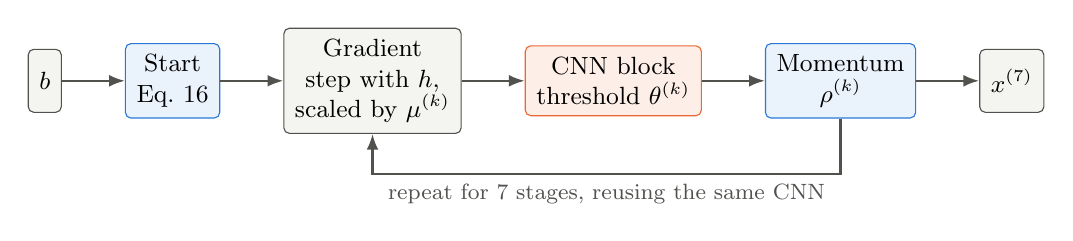
\begin{tikzpicture}[node distance=7mm and 8mm]
\node[fixed] (b) {$b$};
\node[block,right=of b] (init) {Start\\ Eq.~16};
\node[fixed,right=of init] (grad) {Gradient\\ step with $h$,\\ scaled by $\mu^{(k)}$};
\node[learned,right=of grad] (prox) {CNN block\\ threshold $\theta^{(k)}$};
\node[block,right=of prox] (mom) {Momentum\\ $\rho^{(k)}$};
\node[fixed,right=of mom] (out) {$x^{(7)}$};
\draw[flow] (b)--(init); \draw[flow] (init)--(grad); \draw[flow] (grad)--(prox); \draw[flow] (prox)--(mom);
\draw[flow] (mom)--(out);
\draw[flow] (mom.south) -- ++(0,-7mm) -| node[pos=.25,below,note]{repeat for 7 stages, reusing the same CNN} (grad.south);
\end{tikzpicture}
\caption{FISTA-Net. Orange is the shared CNN. $\mu$, $\theta$ and $\rho$ follow learned schedules.}
\end{figure}

\section{Step 1: the starting image, Eq.~16}

\begin{equation}
x^{(0)} = \big(A^TA + \lambda_0 L^TL\big)^{-1} A^T b, \qquad \lambda_0 = 0.001. \tag{Eq.~16}
\end{equation}
$L$ is a matrix of differences between neighbouring pixels. This is a close cousin of Wiener: replace
$\lambda_0L^TL$ with $\mu$ and you get our Wiener filter exactly. Both $A$ and $L$ are convolutions, so each
becomes a simple function of frequency, and the matrix inverse becomes a division.

\begin{code*}{fista_net.py}
def difference_power(n, dtype, device):
    """Fourier symbol of L^T L, with L the row and column differences."""
    fy = torch.fft.fftfreq(n, dtype=dtype, device=device)[:, None]
    fx = torch.fft.rfftfreq(n, dtype=dtype, device=device)[None, :]
    return 4 * (torch.sin(torch.pi * fx) ** 2 + torch.sin(torch.pi * fy) ** 2)
\end{code*}

\begin{code*}{fista_net.py}
    def initial(self, b):
        """Eq. 16: x0 = (A^T A + lambda0 L^T L)^-1 A^T b."""
        n = b.shape[-1]
        h, smooth = self.spectra(n, b)
        return torch.fft.irfft2(torch.fft.rfft2(b) * h / (h * h + smooth), s=(n, n))
\end{code*}

\begin{careful}
The penalty $\lambda_0L^TL$ is very weak at low and middle frequencies, so this start image is far more
aggressive than Wiener. The orange line in Figure~\ref{fig:filters} peaks at a gain of about 80 near a period of
3\um, against Wiener's 2.8. So it starts sharper, and it also amplifies noise much more. The CNN must clean this up.
\end{careful}

\section{Step 2: the gradient module}

This is where the paper and the authors' own code disagree, so this is the first thing I asked you.

\textbf{The paper, Eq.~11--12:} $W^{(k)}=\mu^{(k)}\tilde W$, where $\tilde W$ comes from coherence minimisation.
This is the same weight family as ALISTA.

\textbf{The authors' code, \code{M5FISTANet.py}:}
\begin{equation}
r^{(k)} = y^{(k)} - \mu^{(k)} \big(A^TA + 0.001L^TL\big)^{-1}\big(A^TAy^{(k)} - A^Tb - 0.001L^TLy^{(k)}\big).
\end{equation}

\textbf{You chose the authors' code.} When I asked, I noted that the ALISTA-type weight had amplified noise heavily
on our blur, and that the code's step suits strong blur. Our Fourier form of it:

\begin{code*}{fista_net.py}
    def stage(self, y, b_hat, h, smooth, mu, theta):
        n = y.shape[-1]
        y_hat = torch.fft.rfft2(y)
        step = (h * h * y_hat - h * b_hat - smooth * y_hat) / (h * h + smooth)
        r = y - mu * torch.fft.irfft2(step, s=(n, n))
        return self.block(r, theta)
\end{code*}

\begin{center}
\renewcommand{\arraystretch}{1.4}
\begin{tabular}{ll}
\toprule
Matrix in the code & Fourier form in ours \\
\midrule
$A^TAy$ & \code{h * h * y_hat} \\
$A^Tb$ & \code{h * b_hat} \\
$0.001\,L^TLy$ & \code{smooth * y_hat} \\
$(A^TA + 0.001\,L^TL)^{-1}$ & divide by \code{h * h + smooth} \\
\bottomrule
\end{tabular}
\end{center}

A unit test builds the literal matrices on a small image and confirms that the Fourier version gives the same answer.

\begin{careful}[A sign you should know about]
If you differentiate $\lVert Ay-b\rVert^2+0.001\lVert Ly\rVert^2$, the penalty term comes with a \emph{plus} sign. The authors'
code has a \emph{minus}. Their code comment cites another paper for this formula. Since your instruction was to
follow the authors, we kept the minus, unchanged. I am flagging it so that it does not surprise you. I did not
test the alternative.
\end{careful}

\section{Step 3: the proximal CNN}

\begin{figure}[H]
\centering
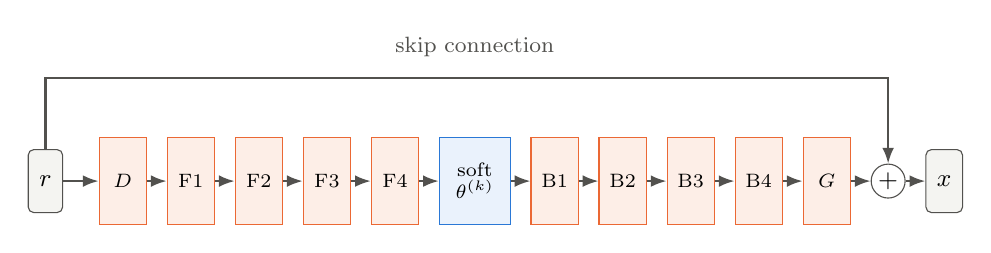
\begin{tikzpicture}[node distance=2.5mm,
 c/.style={draw=warm,fill=warmwash,minimum height=11mm,minimum width=6mm,font=\scriptsize,inner sep=1pt},
 t/.style={draw=accent,fill=bluewash,minimum height=11mm,minimum width=9mm,font=\scriptsize,align=center,inner sep=1pt}]
\node[fixed] (in) {$r$};
\node[c,right=of in,xshift=2mm] (d) {$D$};
\node[c,right=of d] (f1) {F1};
\node[c,right=of f1] (f2) {F2};
\node[c,right=of f2] (f3) {F3};
\node[c,right=of f3] (f4) {F4};
\node[t,right=of f4] (st) {soft\\ $\theta^{(k)}$};
\node[c,right=of st] (b1) {B1};
\node[c,right=of b1] (b2) {B2};
\node[c,right=of b2] (b3) {B3};
\node[c,right=of b3] (b4) {B4};
\node[c,right=of b4] (g) {$G$};
\node[circle,draw=ink,inner sep=1pt,right=of g,font=\small] (plus) {$+$};
\node[fixed,right=of plus] (out) {$x$};
\foreach \p/\q in {in/d,d/f1,f1/f2,f2/f3,f3/f4,f4/st,st/b1,b1/b2,b2/b3,b3/b4,b4/g,g/plus,plus/out} \draw[flow] (\p)--(\q);
\draw[flow] (in.north) -- ++(0,9mm) -| (plus.north);
\node[note,above=9mm of st] {skip connection};
\end{tikzpicture}
\caption{The proximal block. Each orange box is a $3\times3$ convolution with 32 channels. ReLU follows F1--F3 and B1--B3.}
\end{figure}

The paper's text describes 8 convolution layers without bias. But the paper also reports 74,599 parameters, and only the
authors' 10-layer block with bias gives that number:
\begin{equation}
\underbrace{320}_{D:\,1\to32} + \underbrace{8\times9{,}248}_{F,\,B:\,32\to32} + \underbrace{289}_{G:\,32\to1}
+ \underbrace{6}_{w_i,\,c_i} = 74{,}599.
\end{equation}
So you chose the code's 10 layers.

\begin{code*}{fista_net.py}
    def forward(self, r, theta):
        start = self.conv_d(r[:, None])
        coded = self.transform(start)
        kept = torch.sign(coded) * F.relu(torch.abs(coded) - theta)
        output = r + self.conv_g(self.inverse(kept))[:, 0]
        symmetry = ((self.inverse(coded) - start) ** 2).mean()
        return output, symmetry, coded.abs().mean()
\end{code*}

This has the same soft-threshold as everywhere else in this booklet, but it acts on a \emph{learned feature space}, $F$,
not on pixels. $\tilde F$ then maps back. The block has a skip connection, so it learns only a correction to $r$.

\section{Step 4: the learned schedules, Eq.~15}

The paper does not let $\mu$, $\theta$ and $\rho$ float freely. Each follows a formula with two learned numbers, so that it
stays positive and changes smoothly with layer $k$:
\begin{align}
\mu^{(k)} &= \mathrm{sp}(w_1k+c_1), \tag{15a}\\
\theta^{(k)} &= \mathrm{sp}(w_2k+c_2), \tag{15b}\\
\rho^{(k)} &= \frac{\mathrm{sp}(w_3k+c_3)-\mathrm{sp}(w_3+c_3)}{\mathrm{sp}(w_3k+c_3)}, \tag{15c}
\end{align}
where $\mathrm{sp}(x)=\ln(1+e^x)$ is the softplus function. The start values are
$\{w_1,w_2,w_3,c_1,c_2,c_3\}=\{-0.5,-0.2,1,-2,-1,0\}$. Run 1 used these. Run 2 used the authors' code values, as explained
at the end of this chapter.

\begin{code*}{fista_net.py}
    def schedules(self, k):
        """Eq. 15 for iteration k, counted from 1."""
        mu = F.softplus(self.w1 * k + self.c1)
        theta = F.softplus(self.w2 * k + self.c2)
        top = F.softplus(self.w3 * k + self.c3)
        return mu, theta, (top - F.softplus(self.w3 + self.c3)) / top
\end{code*}

\begin{figure}[H]
\centering
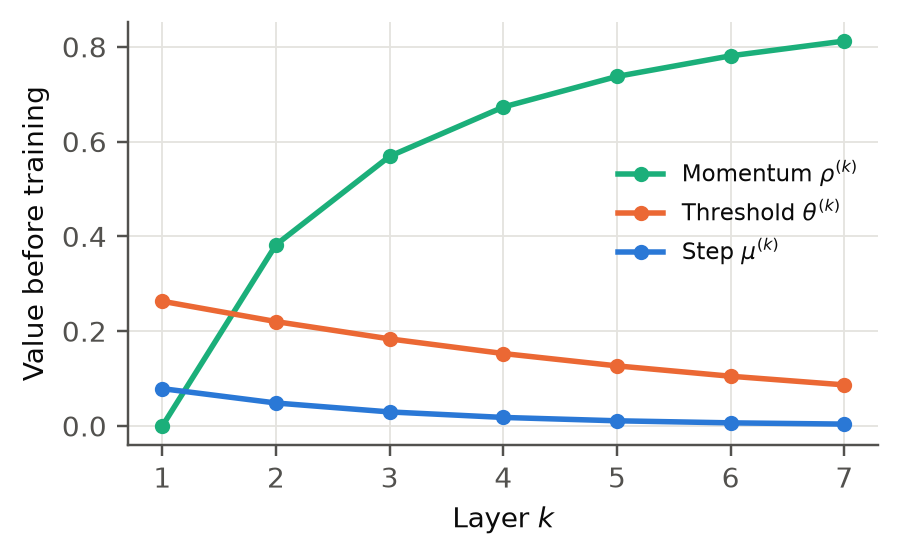
\includegraphics[width=.55\textwidth]{schedules}
\caption{Eq.~15 at the paper's start values, before training.}
\end{figure}

As in FISTA, $\rho$ grows from 0 toward 1. The step and threshold shrink as the image improves. At $k=1$, $\rho=0$
exactly, so the first stage has no momentum.

\section{Step 5: the loss, Eq.~14}

\begin{equation}
L_{\text{total}} = L_{\text{mse}} + \lambda_1 L_{\text{sym}} + \lambda_2 L_{\text{spa}},
\qquad \lambda_1=0.01,\ \lambda_2=0.001 . \tag{Eq.~14}
\end{equation}

\begin{code*}{fista_net.py}
def total_loss(output, target, symmetry, sparsity):
    """Eq. 14 with lambda1 = 0.01 and lambda2 = 0.001."""
    return ((output - target) ** 2).mean() + .01 * symmetry + .001 * sparsity
\end{code*}

\begin{itemize}
\item $L_{\text{mse}}$ compares the final image with the target.
\item $L_{\text{sym}}$ asks $\tilde F$ to undo $F$, so the backward path is a true inverse.
\item $L_{\text{spa}}$ asks the features $F(r)$ to be sparse.
\end{itemize}

\section{The full forward pass}

\begin{code*}{fista_net.py}
    def forward(self, b):
        """b is [B, N, N], zero-padded. Returns field, symmetry and sparsity losses."""
        h, smooth = self.spectra(b.shape[-1], b)
        b_hat = torch.fft.rfft2(b)
        old = y = self.initial(b)
        symmetry = sparsity = 0
        for k in range(1, self.layers + 1):
            mu, theta, rho = self.schedules(k)
            if self.use_checkpoint and self.training:
                x, sym, spa = checkpoint(self.stage, y, b_hat, h, smooth, mu, theta,
                                         use_reentrant=False)
            else:
                x, sym, spa = self.stage(y, b_hat, h, smooth, mu, theta)
            y = x + rho * (x - old)
            old = x
            symmetry, sparsity = symmetry + sym, sparsity + spa
        return x, symmetry, sparsity
\end{code*}

\begin{center}
\renewcommand{\arraystretch}{1.4}
\begin{tabular}{p{6.5cm}p{8cm}}
\toprule
Paper & Code \\
\midrule
$x^{(0)}$, Eq.~16, and $y^{(1)}=x^{(0)}$ & \code{old = y = self.initial(b)} \\
Eq.~15, $k=1\dots N_s$ & \code{self.schedules(k)} \\
Eq.~8a and 8b & \code{self.stage(...)} \\
Eq.~8c & \code{y = x + rho * (x - old)} \\
$\sum_k$ in Eq.~13 & \code{symmetry + sym}, \code{sparsity + spa} \\
Output $x^{(N_s)}$ & \code{return x} \\
\bottomrule
\end{tabular}
\end{center}

\section{Every decision and difference}

\subsection*{Choices you made, when I asked}

\begin{center}
\renewcommand{\arraystretch}{1.3}
\begin{tabularx}{\textwidth}{>{\raggedright\arraybackslash}p{2.8cm}>{\raggedright\arraybackslash}X>{\raggedright\arraybackslash}X>{\raggedright\arraybackslash}p{2.7cm}}
\toprule
Question & Paper & Authors' code & You chose \\
\midrule
Gradient step & $\mu\tilde W$, Eq.~11--12 & Inverse form above & Code \\
CNN & 8 layers, no bias & 10 layers, bias & Code \\
Loss & Eq.~14 & Eq.~14 plus $0.1L_1$ and weight decay & Paper \\
Start values & $\{-0.5,-0.2,1,-2,-1,0\}$ & Different numbers & Paper in run 1, code in run 2 \\
Learning rate & Not given & $10^{-3}$ & Code, without its decay \\
Epochs & Not given & 30 loaded by default & Code \\
\bottomrule
\end{tabularx}
\end{center}

\subsection*{Differences forced by our problem}

\begin{center}
\renewcommand{\arraystretch}{1.3}
\begin{tabularx}{\textwidth}{>{\raggedright\arraybackslash}p{3.3cm}>{\raggedright\arraybackslash}X>{\raggedright\arraybackslash}X}
\toprule
Item & Paper or code & Ours, and why \\
\midrule
Final ReLU & The code forces output $\ge0$ & \textbf{Removed.} Magnetic fields are signed, so it would destroy half the data. This is a real change, and I did not ask you first \\
$A$ and $L$ & Explicit matrices & FFT filters on a padded canvas, because a matrix at this size cannot exist \\
Image size & $64\times64$ EMT images in the paper's first study & 512 pixel crops \\
Batch & 64 & 24, the largest that fits safely \\
Padding & None & 128 pixels of zeros. There is no window mask here, so the gradient step treats the padded zeros as real data \\
\bottomrule
\end{tabularx}
\end{center}

\subsection*{Smaller details that follow the code, not the printed equation}

\begin{center}
\renewcommand{\arraystretch}{1.3}
\begin{tabularx}{\textwidth}{>{\raggedright\arraybackslash}p{3.3cm}>{\raggedright\arraybackslash}X>{\raggedright\arraybackslash}X}
\toprule
Item & Printed Eq.~13 & Ours, following the code \\
\midrule
Symmetry loss & Compares $\tilde F(F(r))$ with $r$ & Compares with the output of \code{conv_D}, $D(r)$, using a mean \\
Sparsity loss & Sum of $\ell_1$ norms & Mean absolute value per layer, summed over layers \\
Layer index & $k=1\dots N_s$ & Same as the paper. The authors' code counts from 0 \\
\bottomrule
\end{tabularx}
\end{center}

\begin{defend}
\textbf{``Did you implement FISTA-Net exactly?''} Say: ``Where the paper and the authors' code disagree, I chose and
recorded which to follow. Two changes are ours: the final ReLU is removed because fields are signed, and the operators
are FFT filters.'' Then point to these tables.
\end{defend}

\section{Training and status}

For run 1: Adam at $10^{-3}$ for everything, no decay, 7 stages, 512 pixel crops, batch 24, 30 epochs. An epoch here means 600 crops,
one per training image, so the run has 750 steps. Validation runs every 25 steps, on the same 64 crops as CSC-LISTA. The
final score uses the same 15 COMSOL pairs. Eight unit tests pass, including the parameter count, Eq.~15, Eq.~16 and the
matrix-versus-Fourier check.

\begin{careful}
Each block of ten $3\times3$ layers sees only 2.1\um\ at 0.1\um\ per pixel, and our wires are about 2\um\ wide. In the paper's
$64\times64$ images, the same block covers a third of the image. The 7 stages together reach 14.1\um, and the gradient
step is global, so this is not a fatal problem. It is simply untested, and it is one thing to look at if the result is poor.
\end{careful}

\section{Run 1: what happened}

\begin{center}
\begin{tabular}{lccc}
\toprule
 & Simulated validation & COMSOL & NRMSE \\
\midrule
Wiener & 60.3\% & 49.3\% & 3.53\% \\
\textbf{FISTA-Net, step 725} & \textbf{65.2\%} & \textbf{39.4\%} & \textbf{2.85\%} \\
Strict Eq.~20, 64 layers & 48.8\% & 33.8\% & 2.43\% \\
\bottomrule
\end{tabular}
\end{center}

The run took 8,332 seconds and peaked at 36.5 GiB. Its 39.4\% was not FISTA-Net's limit, because this run had not
converged.

\begin{figure}[H]
\centering
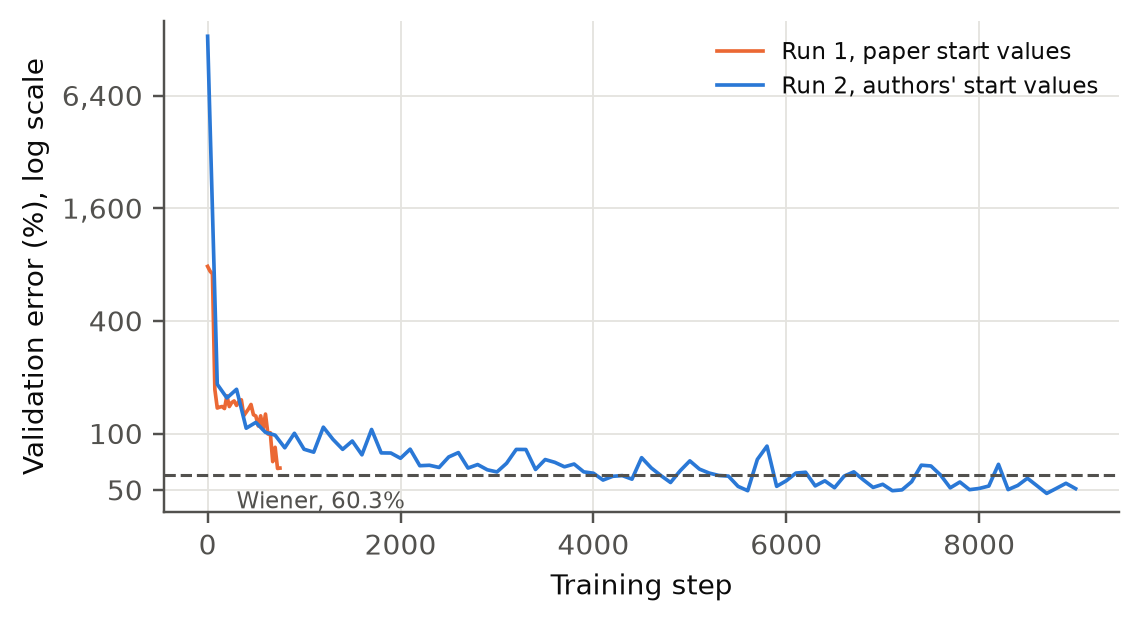
\includegraphics[width=.68\textwidth]{fistanet_curve}
\caption{FISTA-Net validation error during training, for both runs. Run 1 stops at step 750 with no sign of settling.
Run 2 starts far higher and keeps improving for much longer, but it is still noisy at the end.}
\label{fig:fistanet-curve}
\end{figure}

\subsection*{Why the error starts so high}

Before training, the error is 782\%. That comes from the Eq.~16 start image, whose gain of about 80 amplifies the
input noise. A crop with weak signal then gets a huge relative error, and such crops can dominate the mean. This is probably
also why the validation score looks so much worse than the COMSOL score, but I did not test that.

\subsection*{Why I think it stopped short}

\begin{enumerate}
\item \textbf{Far fewer updates.} We trained for 30 epochs of 600 crops at batch 24, which is 750 updates. On the
paper's EMT dataset, 30 epochs at batch 64 would be about 9,000 updates. So ``30 epochs'' was 12 times shorter here.
\item \textbf{The schedules did not learn.} The six scalars barely moved. For example, $w_1$ went from $-0.5$ to $-0.503$, and
$\mu$, $\theta$ and $\rho$ at the last layer stayed at about 0.004, 0.089 and 0.81, so they are effectively still at their
start values.
\item \textbf{The physics step is very small.} See the next section.
\end{enumerate}

\subsection*{A mismatch you should know about}

\begin{careful}[Our start values pair the paper's numbers with the code's gradient step]
You chose the authors' gradient step, and the paper's start values. When I asked, I did not point out how much those
start values differ from the ones in the authors' code, and I should have.
\end{careful}

The authors' code starts $\mu$ at $\mathrm{sp}(0.1-0.2i)$, for $i=0\dots6$. The paper's values give $\mathrm{sp}(-2-0.5k)$.

\begin{center}
\begin{tabular}{lrrrrrrrr}
\toprule
Layer & 1 & 2 & 3 & 4 & 5 & 6 & 7 & Sum \\
\midrule
$\mu$, ours (paper) & 0.079 & 0.049 & 0.030 & 0.018 & 0.011 & 0.007 & 0.004 & 0.197 \\
$\mu$, authors' code & 0.744 & 0.644 & 0.554 & 0.474 & 0.403 & 0.341 & 0.287 & 3.449 \\
\midrule
$\theta$, ours (paper) & 0.263 & 0.220 & 0.184 & 0.153 & 0.127 & 0.105 & 0.087 & \\
$\theta$, authors' code & 0.127 & 0.079 & 0.049 & 0.030 & 0.018 & 0.011 & 0.007 & \\
\bottomrule
\end{tabular}
\end{center}

Summed over the seven stages, our gradient step is about 17 times weaker than in the authors' code, and it never got
larger, because the schedules barely trained. With this inverse-based step, $\mu=1$ would be close to a full jump. Ours adds up to
0.197. So the physics module likely does very little, and the network is mostly a CNN cleaning up the Eq.~16 start image. Our
threshold also starts larger than the code's.

Notice that the paper's $\mu$ numbers, $(-0.5,-2)$, are the numbers the code uses for $\theta$. The paper and the
code may simply have these two labels swapped. I cannot confirm that from the sources.

So run 1 was a fair report of what we ran, but not a fair test of FISTA-Net.

\section{Run 2: the authors' start values and 9,000 updates}

You asked for a rerun. The start values and the length changed, and validation ran less often to keep the cost down.

\begin{center}
\begin{tabular}{lll}
\toprule
 & Run 1 & Run 2 \\
\midrule
Start values & Paper & Authors' code \\
Updates & 750 (30 epochs) & 9,000 (360 epochs) \\
Validation & Every 25 steps & Every 100 steps \\
\bottomrule
\end{tabular}
\end{center}

The code's schedules count from $i=0$ and ours from $k=1$, so the authors' values were rewritten with $c=b-w$. The formula in
Eq.~15 did not change, and a unit test confirms that all seven layers reproduce the authors' $\mu$, $\theta$ and $\rho$.

\begin{code*}{fista_net.py}
START = dict(paper=dict(w1=-.5, w2=-.2, w3=1., c1=-2., c2=-1., c3=0.),
             code=dict(w1=-.2, w2=-.5, w3=.5, c1=.3, c2=-1.5, c3=-.5))
\end{code*}

Everything else stayed the same: the Eq.~14 loss, batch 24, Adam at $10^{-3}$ with no decay, and no final ReLU.

\begin{center}
\begin{tabular}{lccc}
\toprule
 & Simulated validation & COMSOL & NRMSE \\
\midrule
FISTA-Net run 1 & 65.2\% & 39.4\% & 2.85\% \\
FISTA-Net run 2, step 4,800 (interim) & 54.8\% & 34.6\% & 2.50\% \\
\textbf{FISTA-Net run 2, step 8,700} & \textbf{47.9\%} & \textbf{33.3\%} & \textbf{2.41\%} \\
Strict Eq.~20, 64 layers & 48.8\% & 33.8\% & 2.43\% \\
FISTA-300, $\lambda=0.009$ & 35.5\% & 30.5\% & 2.20\% \\
\bottomrule
\end{tabular}
\end{center}

The run took 98,280 seconds, about 27 hours, and also peaked at 36.5 GiB. Fixing the two problems cut the COMSOL error by 6.1
points, and made FISTA-Net the best trained network here, with the fewest parameters.

\subsection*{Reading run 2 honestly}

\begin{itemize}
\item \textbf{It starts much worse.} The first validation error was 13,266\%, against 782\% in run 1. Strong steps
at the start of training amplify the noisy start image further. Training brought this under 115\% by step 500.
\item \textbf{It is still noisy.} In the last 1,000 steps, validation moved between 47.9\% and 68.5\%. The learning rate
never decays, so this may not settle. The best step, 8,700, is partly a lucky draw.
\item \textbf{The schedules still moved little.} At the best step, $\mu$ adds up to 3.166 against the 3.449 it started
from. Most of the learning was in the CNN.
\item \textbf{$B_z$ is its weak spot.} $B_x$ and $B_y$ are at 30.2\% and 30.7\%, better than strict 64 layers, but $B_z$ is at
39.1\%, which is worse. Its worst coil is IC\_4um, at 34.6\%.
\item \textbf{It is not at a limit yet.} Validation was still improving late in the run, so we do not know where it would stop.
\end{itemize}

\begin{keyidea}[What this means]
Our first low score came from our own setup, not from the method. Run 2 is a fair test, and it puts FISTA-Net level with
the much larger CSC-LISTA. It still does not reach FISTA-300's 30.5\%.
\end{keyidea}

The output on the COMSOL crop is in Figure~\ref{fig:reconstruction-new}.

\chapter{Defending this work}\label{ch:defence}

These are the questions most likely to come up, with honest answers.

\begin{careful}[Written on 5 November]
This chapter predates MAGIC-UNet. Its recommendation of FISTA-Net is now superseded on COMSOL score: MAGIC-UNet run 2
scores 27.0\% without being told the standoff. Chapter~\ref{ch:magic_results} has the new questions and answers, and the
limits of that result.
\end{careful}

\section{About the source}

\textbf{What is your network, and where does it come from?}\\
Eq.~20 of Liu, Chen, Wang and Yin, ICLR 2019: convolutional LISTA. The extension to deblurring,
$d_m=h*g_m$, is ours, and no published result covers it.

\textbf{Is it ALISTA?}\\
No. ALISTA computes its weights analytically. We learn ours. Eq.~26 was tried and dropped.

\textbf{Which network do you recommend?}\\
FISTA-Net run 2, from Xiang, Dong and Yang. It has the lowest simulated validation error among runs without our floor and loss
changes, and it scores 33.3\% on COMSOL. Strict Eq.~20 at 33.8\% is effectively tied.

\textbf{Which parts did you invent?}\\
For strict runs: the blurred dictionary, the padding and mask, and the dictionary learning method. Chapter~\ref{ch:differences}
lists all training details. The floor and the relative loss were additions, and strict runs removed them.

\section{About the method}

\textbf{Why not just use FISTA, since it wins?}\\
On accuracy alone, you should. FISTA-300 scores 30.5\%, against 33.3\% for the selected network. Strict Eq.~20 wins at equal
depth, 33.8 against 37.9\% at 64, but only on COMSOL, not on simulated validation. Run time has not been measured, so I
cannot claim any network is faster.

\textbf{Was FISTA tuned fairly?}\\
Yes. Its $\lambda$ came from eight values on 16 simulated crops, and the best one lies inside the grid. COMSOL was not used. The
search was widened after the network scores were known, and you should say so.

\textbf{Did FISTA-Net fail?}\\
Run 1 scored 39.4\%, but it was stopped early and its start values gave a gradient step 17 times weaker than the authors' code.
Run 2 fixed both and scored 33.3\%, so the low score came from our setup. Chapter~\ref{ch:fistanet} has the numbers.

\textbf{Is your network doing sparse coding?}\\
Structurally yes. In behaviour, mostly no. Strict codes have high density, and some thresholds are zero, so it acts
like a learned deconvolution.

\textbf{Does the ALISTA convergence theorem apply?}\\
No. It assumes much sparser codes than ours.

\textbf{Why does $h$ stay fixed?}\\
Because it is physics: upward continuation in a source-free region. We know it exactly, so learning it would only
waste data. The empirical $k_0$ was removed because it breaks harmonicity.

\section{About the data}

\textbf{Why train on simulation?}\\
Only 15 real pairs from two wire shapes exist, far too few for millions of parameters. Simulation derives all
components from one current map, so it is physically consistent.

\textbf{Is the test set really clean?}\\
Models and checkpoints were chosen without COMSOL. But the generator's parameter ranges were designed from these coils,
and we have now compared many methods on them. So it is clean of reconstruction scores, but not completely independent.

\textbf{Why 33.8\% if the method is good? That sounds bad.}\\
Because of how the score works. COMSOL's speckle sets a floor around 15--19\%, the blurry input itself is near 77\% on a
signal-rich crop, and the Wiener filter gets 49.3\%.

\section{About the results}

\textbf{Why did simulated validation disagree with COMSOL?}\\
The simulator differs from COMSOL, for example in its speckle and peaks, and the difference is not fully understood.
The sparse variant won on simulation and lost on COMSOL, so simulated gains do not always transfer.

\textbf{How confident are you in a one-point difference?}\\
Not very. There is one seed per run, and no error bars.

\section{What is not yet known}

\begin{itemize}
\item Where FISTA-Net would settle with a decaying learning rate, or more updates.
\item How stable FISTA-Net's score is across seeds. Its validation error is still noisy.
\item Whether the LFISTA-style network improves at $\lambda=0.009$, or with a higher limit on $\beta$.
\item Actual run times. Without them, no speed claim is possible.
\item Why strict Eq.~20's gain over FISTA at equal depth appears on COMSOL and not on simulated validation.
\item Whether the early validation peak in MSE runs is overfitting or a loss mismatch.
\item Why COMSOL decays faster than free-space physics.
\item Whether results hold on a third wire shape.
\end{itemize}

\chapter{How far can a linear filter go?}\label{ch:floor}

The chapters so far end on 5 November. This chapter and the four after it cover what happened next. Everything here is
still about the 3\um\ to 0.5\um\ problem, unless a section says otherwise.

\section{Why ask this}

Every learned method in Chapter~\ref{ch:results} sat between 30\% and 36\% on COMSOL. Is that close to a hard
limit, or is there a lot of room left? To answer that, we first need the best score a simple \emph{linear} filter could
possibly reach. A linear filter cannot invent anything: it can only boost or damp each frequency that is in the data.

\section{The Wiener filter, fitted on COMSOL}

Our old Wiener baseline was $h/(h^2+\mu)$ with one number $\mu=0.0316$, chosen on simulated data. The real Wiener
filter uses how strong the signal and the noise are at each frequency:
\begin{equation}
W(k) = \frac{H(k)\,S_x(k)}{H(k)^2 S_x(k) + S_n(k)},
\end{equation}
where $H(k)=e^{-k\,\Delta z}$ is the blur, $S_x$ is the power of the sharp field and $S_n$ is the power of the noise.
The script \code{scripts/wiener_oracle.py} measures $S_x$ and $S_n$ from the COMSOL pairs themselves. Here ``noise'' means
whatever the blur model cannot explain: COMSOL's mesh speckle plus any mismatch with free-space physics.

It fits the filter in three ways:
\begin{itemize}
\item \textbf{Oracle:} fitted on the same pairs it is scored on. This is not a usable method; it is a ceiling.
\item \textbf{Other coil:} fitted on one coil, scored on the other.
\item \textbf{Other coil and other heights:} the most honest test.
\end{itemize}

\begin{center}
\begin{tabular}{lc}
\toprule
Filter (local data, two coils, 3\um\ to 0.5\um) & Error \\
\midrule
Old Tikhonov, $\mu=0.0316$ from simulated noise & 49.7\% \\
Scalar $\mu$, fitted on the other coil & 37.3\% \\
Real Wiener, fitted on the other coil & 37.8\% \\
Real Wiener, other coil and other heights & 36.1\% \\
Real Wiener, oracle (ceiling for linear filters) & 34.4\% \\
\midrule
FISTA-300, for reference (15 pairs) & 30.5\% \\
\bottomrule
\end{tabular}
\end{center}

\begin{keyidea}[What the Wiener test showed]
\begin{itemize}
\item The old baseline was badly tuned. Its $\mu$ assumed noise about 18 times stronger than COMSOL really has.
\item Almost all the gain comes from that one number. A single, well-chosen $\mu$ does as well as the full
frequency-shaped filter from 3\um\ up.
\item Even the oracle, at 34.4\%, stays behind FISTA-300 and FISTA-Net. They beat every possible linear filter.
\end{itemize}
\end{keyidea}

\begin{careful}
The fitted Wiener filters saw COMSOL data from another coil; the old $\mu$ saw none. Part of their gain is simply
access to real COMSOL statistics, which a method trained only on simulation does not have. These numbers also come from
the two local coils only. The server rerun with data3 has not been done.
\end{careful}

\section{The lost-band floor}

There is a cleaner way to see the limit. At each frequency, compare the signal that survives the blur with the noise.
Above the frequency where the two are equal (signal-to-noise ratio 1), the data carry no usable information. Now take
the \emph{true} target and delete everything above that frequency. Its error is the \textbf{lost-band floor}: what you
lose if you recover every usable frequency perfectly and invent nothing. The script is
\code{scripts/information_budget.py}.

\begin{center}
\small
\begin{tabular}{lccccc}
\toprule
Input height (\textmu m), target 0.5\um & 1 & 2 & 3 & 4 & 5 \\
\midrule
Floor, L1\_C1 & 17.5\% & 21.0\% & 33.4\% & 39.8\% & 41.3\% \\
Floor, IC\_4um & -- & -- & 35.6\% & 42.6\% & 52.4\% \\
Wiener oracle, mean of coils & 18.0\% & 23.8\% & 34.4\% & 41.2\% & 45.9\% \\
\midrule
Input height (\textmu m) & 6 & 7 & 8 & 9 & 10 \\
\midrule
Floor, L1\_C1 & 42.6\% & 44.8\% & 47.4\% & 53.6\% & 56.0\% \\
Floor, IC\_4um & 58.2\% & 65.4\% & -- & -- & 73.5\% \\
Wiener oracle, mean of coils & 51.0\% & 56.7\% & 50.3\% & 55.3\% & 72.8\% \\
\bottomrule
\end{tabular}
\end{center}

Heights 1, 2, 8 and 9\um\ exist for L1\_C1 only, so their oracle row covers one coil. IC\_4um is harder at every height.

At 3\um\ the floor over both coils is 34.5\%, the same as the Wiener oracle. That is no coincidence: the Wiener filter is
close to ``keep the usable band, drop the rest''.

\begin{keyidea}[The most important number in these chapters]
At 3\um\ to 0.5\um, about a third of the target lies in frequencies the data cannot see. Any method that scores below
34.5\% must be \emph{filling in} those frequencies from a prior: an idea of what sources look like. FISTA does this with its
dictionary, and MAGIC-UNet (Chapter~\ref{ch:magic_results}) with what it learned from simulated wires. From 4\um\ up, 40 to
70\% of the target must come from the prior. So at large standoffs the prior matters more than the algorithm.
\end{keyidea}

\begin{defend}[If your professor asks: why are all the scores near 30\%?]
Because a third of the target is not in the measurement at all. The lost-band floor at 3\um\ is 34.5\%, and the best
linear filter reaches 34.4\%. FISTA-300 (30.5\%) and MAGIC-UNet (27.0\%) beat it only because their priors fill in part of
the lost band.
\end{defend}

\chapter{Two more tests of CSC-LISTA}\label{ch:followups}

Chapter~\ref{ch:results} left two open questions about strict Eq.~20 at 64 layers. Its simulated validation error was
best very early (step 200 of 1,000) and then got worse. Was it overfitting the 200 stored layouts? And does training on
MSE, when we score relative $L_2$, hold it back? On 6 November we ran one test for each. Both kept everything else
strict: same dictionary, same 64 layers, same 1,000 steps of 8 crops of 512 pixels.

\section{Test 1: a new layout for every crop}

The trainer gained a \code{--stream} option. Instead of cutting crops from the 200 stored layouts, it simulates a brand-new
current layout for every crop. Over 1,000 steps of 8 crops that is 8,000 layouts, so the network never sees the same wires
twice. If the early peak were overfitting, it should disappear.

\section{Test 2: the relative loss, and nothing else}

The second test switched only the loss to per-crop relative $L_2$, the same quantity we score. This is \textbf{our
addition}, not part of Eq.~20. The earlier relative runs in Chapter~\ref{ch:density} also had the threshold floor, so this
was the first clean test of the loss alone. It ran on the stored layouts and again with streaming.

\section{Results}

\begin{center}
\begin{tabular}{lcc}
\toprule
Strict Eq.~20, 64 layers & Simulated validation & COMSOL (15 pairs) \\
\midrule
MSE, 200 stored layouts (Chapter~\ref{ch:results}) & 48.8\% & \textbf{33.8\%} \\
MSE, 8,000 streamed layouts & 49.3\% & 36.0\% \\
Relative loss, 200 stored layouts & 41.0\% & 35.6\% \\
Relative loss, 8,000 streamed layouts & \textbf{40.9\%} & 36.2\% \\
\bottomrule
\end{tabular}
\end{center}

\begin{figure}[H]
\centering
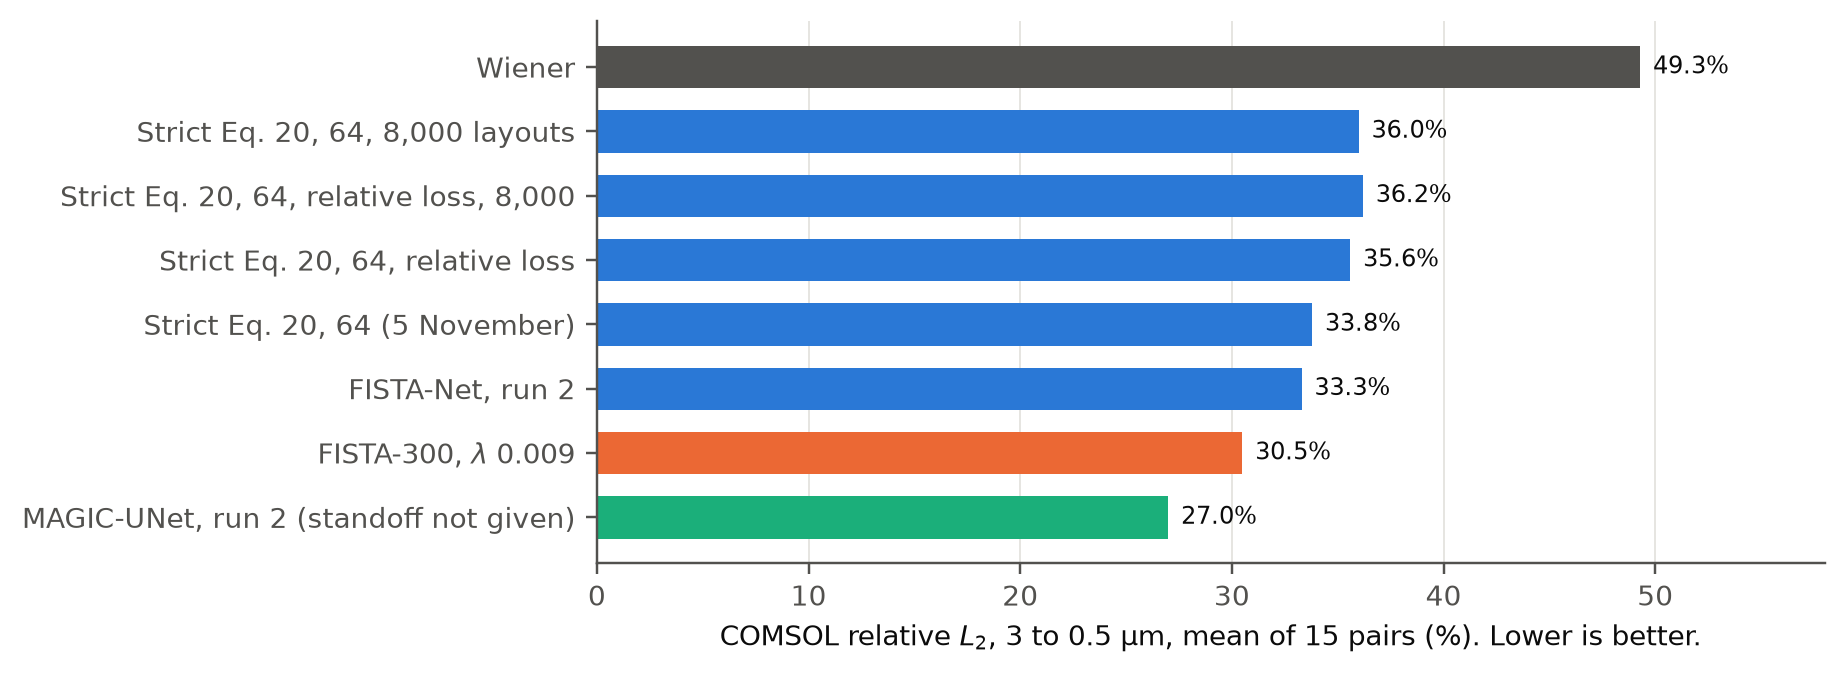
\includegraphics[width=\textwidth]{results_now}
\caption{COMSOL scores at 3\um\ to 0.5\um\ after 5 November, with the earlier best results for comparison. Blue bars are
CSC-LISTA and FISTA-Net, orange is FISTA, green is MAGIC-UNet (Chapters~\ref{ch:magic} and~\ref{ch:magic_results}).}
\label{fig:results_now}
\end{figure}

\begin{keyidea}[What the two tests mean]
\begin{itemize}
\item \textbf{More data did not help.} With 8,000 layouts the validation error still peaked early (step 100) and then
rose. So the early peak is not overfitting. It is a mismatch between the training loss and the score.
\item \textbf{The relative loss fixed that mismatch on simulation:} validation fell from 48.8\% to 41.0\%. But COMSOL got
\emph{worse}, 35.6\% against 33.8\%.
\item So the limit is neither data volume nor the loss. It is the gap between our simulator and COMSOL. Making the network
better at simulated data made it slightly worse at COMSOL.
\end{itemize}
\end{keyidea}

\begin{careful}
Each run used one seed, and the COMSOL differences are about 2 points. That is enough to say these changes did not help,
but not enough to rank the four runs against each other.
\end{careful}

\begin{defend}[If your professor asks: did you try more training data?]
Yes. A fresh simulated layout for every crop, 8,000 in all, gave 36.0\% on COMSOL against 33.8\% with 200 layouts. Data
volume is not what limits CSC-LISTA.
\end{defend}

\chapter{The full research question}\label{ch:question}

The one-standoff restart was a starting point, not the goal. On 7 November you restated the actual question:

\begin{keyidea}[The research question]
Can a physics-based learned inverse estimate unknown standoff and reconstruct near-plane QDM magnetic fields
consistently across unseen geometries, fields of view and sampling scales?
\end{keyidea}

A paper on this would need to show:
\begin{enumerate}
\item joint standoff estimation and field reconstruction, with a distinct inference method;
\item generalisation to unseen geometries, fields of view, pixel spacings and noise levels;
\item how the method handles the ambiguity between source and height, for example with uncertainty or competing
hypotheses;
\item ideally, evidence on experimental QDM data.
\end{enumerate}

This chapter collects what we found when we looked at the question as a whole. Nothing in it was trained.

\section{An exact ambiguity}

Model the source as a thin current sheet at depth $h$ below the sensor. Every field component then has the form
\begin{equation}
B(k) = \tfrac{\mu_0}{2}\,e^{-kh}\,K(k)\,g(k),
\end{equation}
where $g$ describes the current and $K$ is a fixed factor that depends only on direction. Now move the sheet down by
$\delta$ and make it sharper by $e^{k\delta}$:
\begin{equation}
e^{-k(h+\delta)}\,K(k)\,\big(g(k)\,e^{k\delta}\big) = e^{-kh}\,K(k)\,g(k).
\end{equation}
\textbf{The measurement is identical.} A source at depth $h$ and a sharper source at depth $h+\delta$ cannot be told apart
from the field alone. Measuring $B_x$, $B_y$ and $B_z$ does not help, because all three share the same $e^{-kh}$.

\begin{keyidea}[What follows from it]
\begin{itemize}
\item \textbf{The height cannot come from the field alone.} Only a prior on what sources look like (sharp wire edges,
smooth currents, no ringing) can pick one depth.
\item \textbf{The two hypotheses predict different near-plane fields.} So a wrong height directly spoils the
reconstruction. Height and reconstruction are one problem.
\item \textbf{Where the prior is weak, the honest answer is a set of heights,} each with its own reconstructed field.
That is the direct answer to ``how do you handle the ambiguity''.
\end{itemize}
\end{keyidea}

\begin{careful}
``Standoff'' here means the \emph{effective} depth of the sheet. The thickness of the NV layer, the thickness of the
conductor and the optical blur all add to it. A paper should report the physical gap and the effective depth separately.
\end{careful}

\section{Can the spectrum tell the height?}

A tempting shortcut is to read the height off the slope of the field's power spectrum, since $|B|^2$ falls like
$e^{-2kh}$. We tried it on our COMSOL pairs.
\begin{itemize}
\item \textbf{With the fitting band chosen using the true height} (cheating): IC\_4um came out 0.2--0.6\um\ too high, but
L1\_C1 above 4\um\ came out 1--5\um\ too low; 10\um\ read as 5.2\um. The coil's own spectrum fights the exponential.
\item \textbf{With the band chosen from the data alone:} every height above 3\um\ read as 0.9--2\um, because COMSOL's
speckle is not white noise and leaks into the band.
\end{itemize}
Both failures are the ambiguity above in action: the answer depends on what the source looks like. The height has to
come from a source prior together with the reconstruction.

\section{What others have done}

\begin{center}
\small
\begin{tabularx}{\textwidth}{>{\raggedright\arraybackslash}p{4.2cm}X}
\toprule
Work & What it offers us \\
\midrule
NV practice (several papers) & Standoff fitted on a known feature: a wire profile, a film edge, a dipole. This is how
the real QDM could be calibrated. \\
Setescak et al.\ 2026 & Fits the sensor distance jointly with the magnetisation, using an energy prior. The closest prior
work, but for magnetisation, not learned, and with no uncertainty. \\
MAGIC-UNet, Reed et al.\ 2025 & A U-Net from field to current, trained over a range of standoffs that it is never told.
Chapters~\ref{ch:magic} and~\ref{ch:magic_results}. \\
Dubois et al.\ 2022 & An untrained network whose loss is the exact forward model. No training data, so no simulator gap. \\
USRNet, DPIR & One unrolled network for many blur kernels, scales and noise levels, given the kernel. \\
IKC, DAN & Alternate between estimating the blur and restoring the image. \\
BlindDPS, Fast Diffusion EM & A diffusion prior on the image, with the blur parameters estimated alongside. \\
\bottomrule
\end{tabularx}
\end{center}

\begin{keyidea}[The gap]
We found no learned method that estimates the standoff jointly with the reconstruction, reports competing heights, or is
tested across pixel spacing and field of view. The blind-deblurring literature has the machinery; nobody has applied it to
magnetic imaging. Our blur has only one unknown, the height, so a much more careful treatment is possible than in general
blind deblurring.
\end{keyidea}

\begin{careful}[Where these summaries come from]
Some entries were read in full; others come only from abstracts. Read the full papers before quoting any of them. The
survey with sources is \code{RESEARCH_BEYOND_ISTA.md}.
\end{careful}

\section{A candidate method, and the first test}

One design that fits the question:
\begin{enumerate}
\item For each candidate depth $h_j$ on a grid, run one shared reconstructor that is told $h_j$.
\item Score each pair $(h_j, x_j)$ by how well it fits the data and how plausible the source is.
\item Report the spread of supported heights, with one field for each. Give a single answer only when one height clearly
wins.
\item Refine the height around the best candidate.
\end{enumerate}
Every component of this is published (USRNet, DAN, BlindDPS); the combination and the treatment of the ambiguity would be
new. That keeps the professor's rule: published parts and baselines, with a clearly labelled contribution.

Before building any of it, one cheap check decides whether joint estimation can work at all. On COMSOL, fit a regularised
current at each candidate height and see whether the best fit lands on the true height. If no prior puts the minimum near
the truth, the height must be calibrated externally, and that is itself a result. This check has not been run yet.

\begin{defend}[If your professor asks: why not just estimate the height from the data?]
Because the data alone cannot fix it. A source at depth $h$ and a sharper one deeper down give exactly the same field. Our
spectral test on COMSOL confirmed it: the estimates were off by up to 5\um. Height can only come from a prior on sources,
and the method has to say how sure it is.
\end{defend}

\chapter{MAGIC-UNet: the paper and our copy}\label{ch:magic}

\section{The paper}

N. R. Reed, D. Bhutto, M. J. Turner, D. M. Daly, S. M. Oliver, J. Tang, K. S. Olsson, N. Langellier, M. J. H. Ku,
M. S. Rosen and R. L. Walsworth, ``Machine learning for improved current-density reconstruction from two-dimensional
vector magnetic images'', \emph{Physical Review Applied} \textbf{23}, 034035 (2025), doi:10.1103/PhysRevApplied.23.034035.
The preprint is arXiv 2407.14553 (2024). The network is a U-Net, and the authors call it MAGIC-UNet (Magnetic Inverse
Calculation UNet).

\begin{keyidea}[How to read the first half of this chapter]
Everything up to Section~\ref{sec:magic_sources} is taken from the published paper, and each statement names the section,
table or figure it comes from, so you can check it. Where the paper is silent, the text says so. Our own calculations are
marked \emph{ours}. Older notes in this repository cite a ``Supplement D''. The published version has no supplement. Its
recipe is in Sec.~V~A, Tables IV and V, and Appendix~A, and its noise analysis is in Appendix~B. Cite those.
\end{keyidea}

\section{The problem they set out to solve}

A QDM measures the vector field $(B_x, B_y, B_z)$ in a plane some distance above a sample. The wanted output is the
planar current density $(J_x, J_y)$ that made it (Sec.~II). The standard tool is the \emph{Fourier method}: invert the
Biot--Savart law in Fourier space. The paper's introduction names its two weak spots (Sec.~I): noise at high spatial
frequency, and a standoff larger than the size of the current features. The workaround is to average many repeated
measurements, which is slow and lets drift creep in.

Why both weak spots are the same problem: for a thin current sheet a distance $z$ below the sensor, every Fourier
component of the field is the matching component of the current times a fixed factor:
\begin{equation}
\hat B(\bm k, z) \;\propto\; \frac{\mu_0}{2}\, e^{-kz}\, \hat J(\bm k), \qquad k = |\bm k|.
\label{eq:magic_decay}
\end{equation}
The paper does not print this equation. For the Fourier transformations it uses, it cites its refs.~[30,~59] (Roth
2023; Broadway et al.\ 2020) in Sec.~V~C. Its ref.~[37] (Roth, Sepulveda and Wikswo 1989) is cited where Sec.~I says the
Fourier method fails on noisy data. Inverting means multiplying by $e^{+kz}$, so noise at large $k$ is amplified
exponentially.

\begin{keyidea}[How bad the amplification is (ours, from Eq.~\ref{eq:magic_decay})]
At the finest scale an image can hold, $k = \pi/\Delta$ for pixel size $\Delta$, the gain is $e^{\pi z/\Delta}$.
\begin{center}
\small
\begin{tabular}{lcccc}
\toprule
Case & $z$ & $\Delta$ & $z/\Delta$ & $e^{\pi z/\Delta}$ \\
\midrule
Paper, main model & 50\um & 31\um & 1.6 & $1.5\times10^{2}$ \\
Paper, large-standoff model & 500\um & 31\um & 16 & $7\times10^{21}$ \\
Ours, run 2 & 3\um & 0.2\um & 15 & $3\times10^{20}$ \\
Ours, 10\um\ runs & 10\um & 0.7\um & 14 & $3\times10^{19}$ \\
\bottomrule
\end{tabular}
\end{center}
Measured in pixels, our problem is like the paper's \emph{large-standoff} case, not its main one. Keep this in mind for
Section~\ref{sec:magic_limits}.
\end{keyidea}

\section{The question this paper settles: is the network told the standoff?}\label{sec:magic_standoff}

No. Three places in the paper say so:
\begin{enumerate}
\item \textbf{Sec.~III, second paragraph.} The synthetic validation images each have a standoff drawn from a normal
distribution with mean 50\um\ and standard deviation 10\um, chosen to mimic the spread of a real experiment. The Fourier
method is given the exact standoff of each image. MAGIC-UNet is not, and the authors call that a practical feature for
experiments.
\item \textbf{Table V.} The standoff is $50\pm10$\um\ for both wire classes in the training and validation data, and
$500\pm50$\um\ for the large-standoff model.
\item \textbf{Sec.~V~C.} The same distribution, mean 50\um\ and standard deviation 10\um, is described as approximating
the real separation between the NV layer and the current traces in their circuit board.
\end{enumerate}

\begin{careful}[What this means for our claims]
``A network that reconstructs the current without being told the standoff, inside a band of about $\pm20\%$'' is the
paper's result, not ours. Do not present it as new. The paper does \emph{not}:
\begin{itemize}
\item use one network across very different standoffs. The 500\um\ case is a \emph{separate} network trained at
$500\pm50$\um\ (Sec.~III~C, Table~V);
\item output a standoff, or an uncertainty;
\item give the field at another height. It stops at the current.
\end{itemize}
Also note the comparison in the paper is generous to the baseline. The Fourier method gets the exact standoff and a
tuned filter (Section~\ref{sec:magic_fourier}); MAGIC-UNet gets neither.
\end{careful}

The standoffs actually tested sit inside or near the training band: 40$\pm$5\um\ for the noise sweep (Fig.~3), 65\um\ and
36\um\ for the experimental images of Fig.~4, 45\um\ for the Hilbert-curve images of Fig.~5, and about 500\um\ for the
large-standoff network (Fig.~6). The experimental standoffs ranged over 36--65\um\ and 486--650\um\ (Sec.~V~B).

\section{Training data (Sec.~V~A, Appendix~A, Table~V)}

The current comes first, the field second. Random wire shapes are drawn, then COMSOL and MATLAB finite-element runs give
the current density that flows when a voltage is put across the conductor, so the current bends around corners
realistically (Sec.~V~A, Fig.~8). The field is then computed from that current with the Biot--Savart law written as a
Fourier transform, with no noise at this stage (Appendix~A).

\begin{center}
\small
\begin{tabularx}{\textwidth}{>{\raggedright\arraybackslash}p{3.4cm}>{\raggedright\arraybackslash}X>{\raggedright\arraybackslash}X}
\toprule
Parameter (Table V) & Class I & Class II \\
\midrule
Wires & Curves through 2--21 random points (cropped); can loop and short when they cross & Thin right-angle segments,
thin segments at any angle, thick straight wires \\
Independent wires & 1 & 1, 2 or 3 (closely spaced planes) \\
Field of view & 2\,mm & 2\,mm \\
Standoff & $50\pm10$\um\ ($500\pm50$\um\ large standoff) & $50\pm10$\um\ ($500\pm50$\um\ large standoff) \\
Current layer & 14\um\ thick & 14\um\ thick \\
Wire width & 16--160\um\ (50\%), 160--320\um\ (50\%) & 9--30\um\ (67\%), 97--156\um\ (33\%) \\
Current & 15.5--311\,mA & 1.95--170\,mA \\
\bottomrule
\end{tabularx}
\end{center}

\begin{itemize}
\item \textbf{Size.} 153{,}600 training pairs and 4{,}096 pairs for validation and testing (Sec.~V~A). Images are
$64\times64$, so a 2\,mm view gives pixels of about 31\um, the same as their binned experimental images (Sec.~V~B).
\item \textbf{Augmentation.} A $90^\circ$ rotation, a horizontal flip and a vertical flip, each applied with probability
1/2, giving eight variants (Appendix~A).
\item \textbf{Fields from outside.} About 2\% of the training images have wires only outside the field of view, so the
network learns what fields from outside look like (Appendix~A).
\item \textbf{Scaling.} Each input image $i$ is divided by its own scalar $\alpha_i$, and its target current by the same
$\alpha_i$. All targets are also multiplied by one global $\beta\approx10^{8}$, which is divided out after prediction
(Appendix~A). The paper does \emph{not} say how $\alpha_i$ is computed.
\item \textbf{Noise.} Fresh additive Gaussian noise is drawn between every epoch (Appendix~A). The authors chose it after
measuring their real noise (Appendix~B, Section~\ref{sec:magic_limits}). The training noise level is \emph{not} stated.
\end{itemize}

\section{The network (Sec.~II, Fig.~1)}

\begin{figure}[H]
\centering
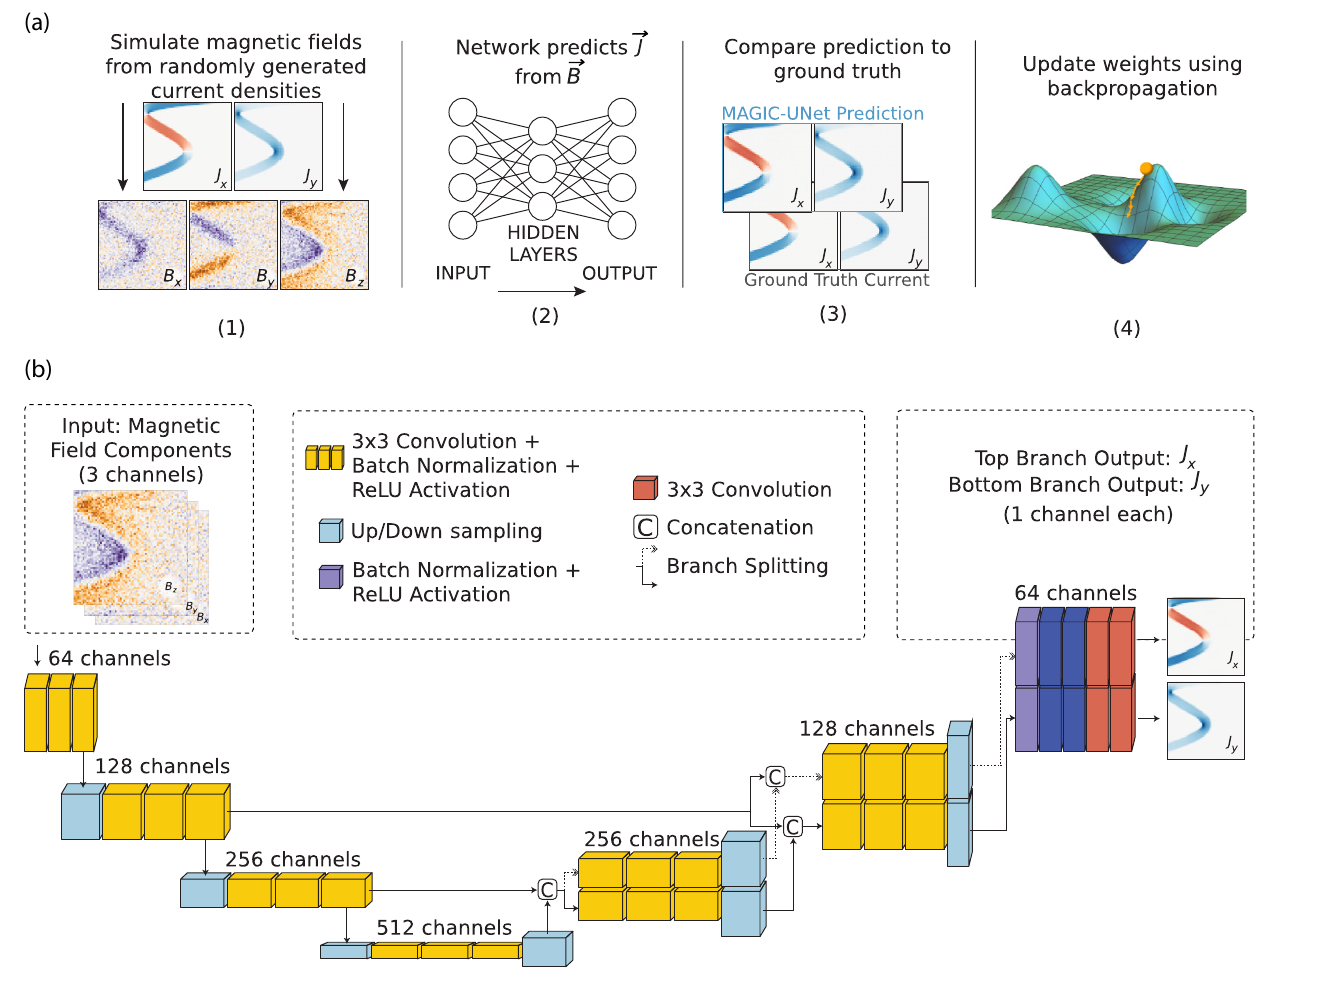
\includegraphics[width=\textwidth]{reed_fig1}
\caption{(a) The training loop: simulate fields from random currents, predict, compare by mean squared error, update by
backpropagation. (b) MAGIC-UNet. Yellow: $3\times3$ conv, BatchNorm, ReLU. Light blue: down- or upsampling. Purple:
BatchNorm and ReLU. Red: $3\times3$ conv. The two output branches, one for $J_x$ and one for $J_y$, never interact.
\emph{Source:} Reed et al., Phys.\ Rev.\ Applied \textbf{23}, 034035 (2025), Fig.~1, CC BY 4.0; cropped, otherwise
unchanged.}
\label{fig:reed_fig1}
\end{figure}

What Sec.~II says, step by step:
\begin{enumerate}
\item \textbf{Encoder.} At each level, a padded $3\times3$ conv, BatchNorm and ReLU, three times, then $2\times2$
average pooling. The text says ``a stride of 1''; see Section~\ref{sec:magic_sources} for why we use 2. The resolution
halves and the channels double at each of three steps: 64, 128, 256, then 512 at the bottom.
\item \textbf{Why average pooling.} Max pooling keeps only the strongest pixel. Every detail of the field matters here, so
they average.
\item \textbf{Skips.} Encoder outputs are concatenated with the decoder at the same resolution. The first (64-channel)
skip is left out because it did not help.
\item \textbf{Two decoders.} After the bottom, the network splits. Each branch upsamples by $2\times2$ with a convolution,
concatenates the skip, and applies conv, BatchNorm and ReLU three times. One branch outputs $J_x$, the other $J_y$. Read
literally that is four convolutions per decoder level; Section~\ref{sec:magic_sources} explains why the released model
has three.
\end{enumerate}

\section{Training (Table~IV)}

\begin{center}
\small
\begin{tabular}{lllllll}
\toprule
Optimiser & Learning rate & Epochs & Batch & Loss & Library & GPU \\
\midrule
RMSprop & $10^{-4}$ & 50 & 32 & MSE & TensorFlow 2.10.0 & RTX A6000, 48\,GB \\
\bottomrule
\end{tabular}
\end{center}

Training took 11 hours (Table~IV). Why MSE: it is the maximum-likelihood loss for Gaussian noise, which is what they
measured in real data (Sec.~III~A).

\section{The baseline they beat: a tuned Fourier method (Sec.~V~C)}\label{sec:magic_fourier}

The authors did not compare against a naive inversion. They tuned it:
\begin{itemize}
\item they use $B_x$ and $B_y$ rather than $B_z$, which is more robust (following Broadway et al.\ [59]);
\item they apply a Gaussian filter against aliasing and the finite Fourier bandwidth, and a Hann window against noise
(the Hann window following their ref.~[37]);
\item they search the window and filter strengths in three dimensions, for several standoffs, to maximise SSIM on
synthetic data;
\item and they give it the exact standoff of each image (Sec.~III).
\end{itemize}

\section{How they measure noise and quality (Sec.~III, Appendix~C)}

\textbf{Noise level.} The noise is set relative to the strongest field in the image:
\begin{equation}
\sigma_n = \frac{\sigma}{\max_{\text{pixels}} |\bm B|}.
\label{eq:magic_sigma_n}
\end{equation}
That is, Gaussian noise of standard deviation $\sigma = \sigma_n \max|\bm B|$ is added to the field.
So $\sigma_n = 0.2$ means a noise standard deviation of one fifth of the peak field. The paper relates $\sigma_n = 0.5$
to an input SNR of about 2, and $\sigma_n = 1$ to SNR about 1.

\textbf{SNR of real images} (Appendix~C). Along a strong wire segment, take the peak field on each line cut across it and
average those peaks. Divide by the standard deviation of the pixels in a quiet region.

\textbf{Quality.} SSIM (structural similarity) is the main score, with the rule of thumb they quote: 0.95--0.99 is close
to perfect, 0.88--0.95 is fair, below 0.88 is poor, below 0.50 is bad (Sec.~III, refs.~[52,~53]). They also report RMSE
and PSNR.

\section{What they found}

\begin{figure}[H]
\centering
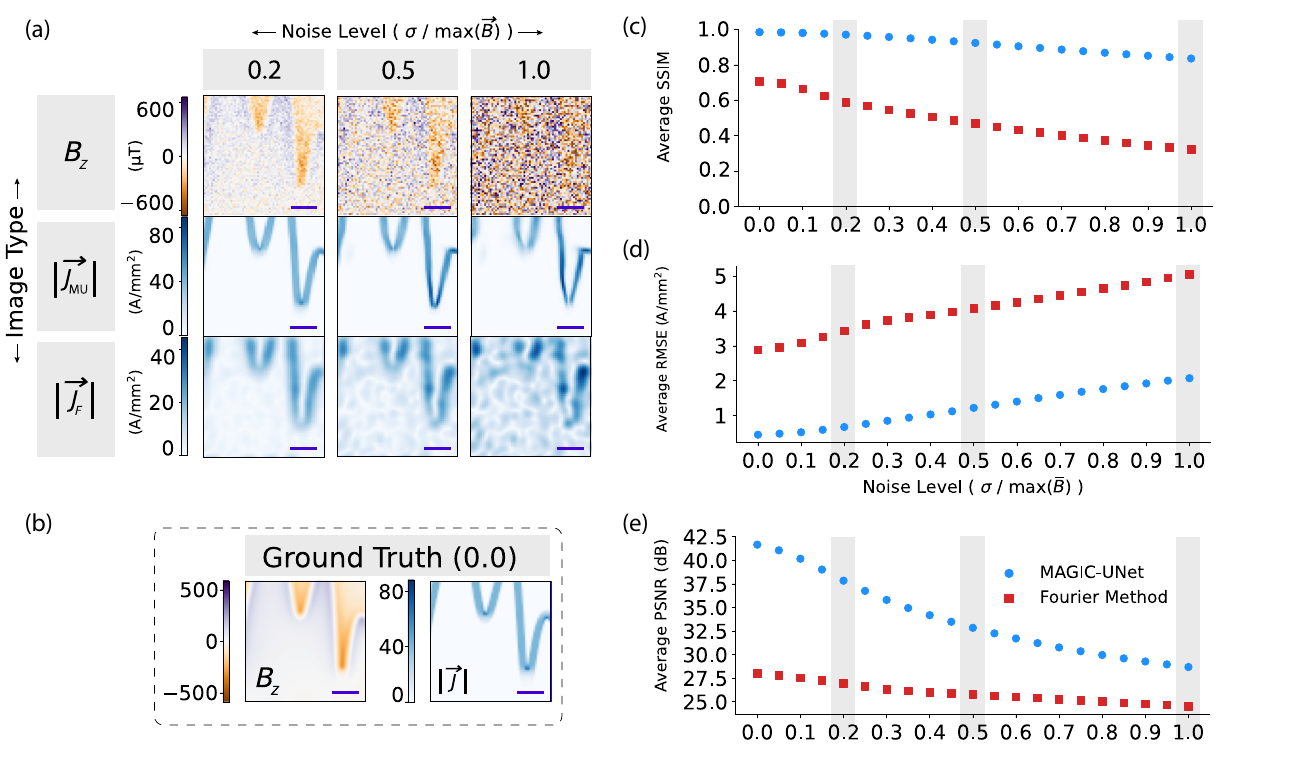
\includegraphics[width=\textwidth]{reed_fig3}
\caption{The noise sweep, at standoff $40\pm5$\um. (a) $B_z$ at $\sigma_n = 0.2$, 0.5 and 1.0, with the current magnitude
from MAGIC-UNet (middle row) and from the Fourier method (bottom row). (b) The truth. (c)--(e) Average SSIM, RMSE and PSNR
against $\sigma_n$: MAGIC-UNet blue circles, Fourier method red squares. \emph{Source:} Reed et al., Phys.\ Rev.\ Applied
\textbf{23}, 034035 (2025), Fig.~3, CC BY 4.0; cropped, otherwise unchanged.}
\label{fig:reed_fig3}
\end{figure}

\begin{center}
\small
\begin{tabular}{lcc}
\toprule
Score, from $\sigma_n = 0$ to $\sigma_n = 1$ (Fig.~3, Sec.~III~A) & MAGIC-UNet & Fourier method \\
\midrule
SSIM & 0.99 $\to$ 0.84 & 0.71 $\to$ 0.32 \\
PSNR & 41.7 $\to$ 28.7\,dB & 28.0 $\to$ 24.5\,dB \\
RMSE & \multicolumn{2}{c}{Fourier about 3--4 times larger at every level} \\
\bottomrule
\end{tabular}
\end{center}

\begin{itemize}
\item MAGIC-UNet stays above SSIM 0.95 up to $\sigma_n = 0.35$ (SNR above 2.8), and above 0.88 for $\sigma_n$ between
0.40 and 0.70 (Sec.~III~A).
\item Sec.~IV quotes a different comparison, for the $64\times64$ network at 50\um\ (Fig.~3 is at $40\pm5$\um): the
RMSE is about 10 times lower than the Fourier method's without noise, and about 2.5 times lower at
SNR 1. MAGIC-UNet at $\sigma_n = 1$ beats the Fourier method at $\sigma_n = 0$ on all three scores (Sec.~IV). Their
headline: SNR-1 inputs to MAGIC-UNet were more accurate than SNR-20 inputs to the Fourier method, which means data
collected 400 times faster.
\item By wire class (Table I), MAGIC-UNet SSIM is 0.895--0.962, against 0.356--0.519 for the Fourier method. $J_x$ and
$J_y$ are equally good (within 1\%).
\item Out of distribution: COMSOL-made straight and curved wires reach SSIM 0.962 at $\sigma_n = 0.5$. Branching wires of
uneven width reach only 0.88, so the network ``has not learned a fully general version of the inversion'' (Sec.~III~A).
\item Larger images (Sec.~III~B, Table~III). A separate $256\times256$ network beats the $64\times64$ one at high noise
on synthetic data (SSIM 0.923 against 0.836 at $\sigma_n = 1$), but is worse on noisy experimental data. Tiling with the
$64\times64$ network works well: overlapping $64\times64$ tiles, overlaps divided equally between neighbours,
duplicates discarded (Fig.~5c). It works even when a tile covers a field of view four times smaller than the training
images.
\end{itemize}

\section{Their limits, from the paper}\label{sec:magic_limits}

\subsection{Correlated noise in real data (Appendix~B)}

\begin{figure}[H]
\centering
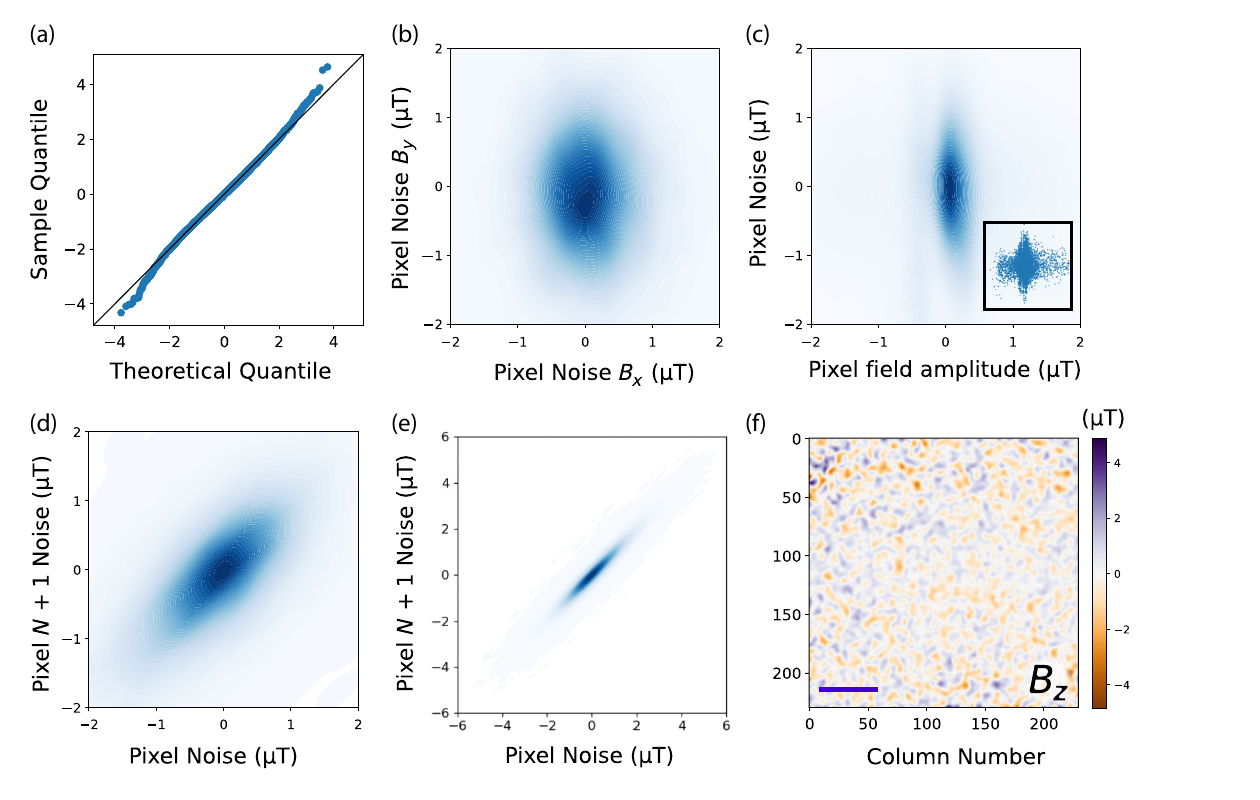
\includegraphics[width=\textwidth]{reed_fig10}
\caption{Noise in real QDM images, from low-SNR minus high-SNR maps of the same view. (a) Quantile plot: close to
Gaussian. (b) $B_x$ noise against $B_y$ noise: uncorrelated. (c) Noise against field amplitude: additive, not growing
with the field. (d), (e) Each pixel's noise against its neighbour's, at $64\times64$ and $230\times230$: strongly
correlated. (f) A $B_z$ noise map with blobs 5--10 pixels wide. \emph{Source:} Reed et al., Phys.\ Rev.\ Applied
\textbf{23}, 034035 (2025), Fig.~10, CC BY 4.0; cropped, otherwise unchanged.}
\label{fig:reed_fig10}
\end{figure}

Real QDM noise is Gaussian, additive and uncorrelated between components, so white Gaussian training noise is a
reasonable model, except in one respect: neighbouring pixels are correlated, $R^2 = 0.60$ at $64\times64$ and
$R^2 = 0.95$ at $230\times230$. The authors blame the ODMR fitting step. MAGIC-UNet shows more artefacts on real images
than on synthetic ones at the same $\sigma_n$ (Sec.~III, Fig.~4). Their two suggested fixes: reduce the correlation in the
measurement, or put correlation into the training noise. Our \code{--noise-corr-um} ablation is the second fix.

\subsection{Several current planes (Table~II)}

SSIM falls from 0.966 with one plane to 0.902 with two and 0.842 with three closely spaced planes. The Fourier method
stays near 0.41 throughout.

\subsection{Large standoff (Sec.~III~C, Fig.~6)}

\begin{figure}[H]
\centering
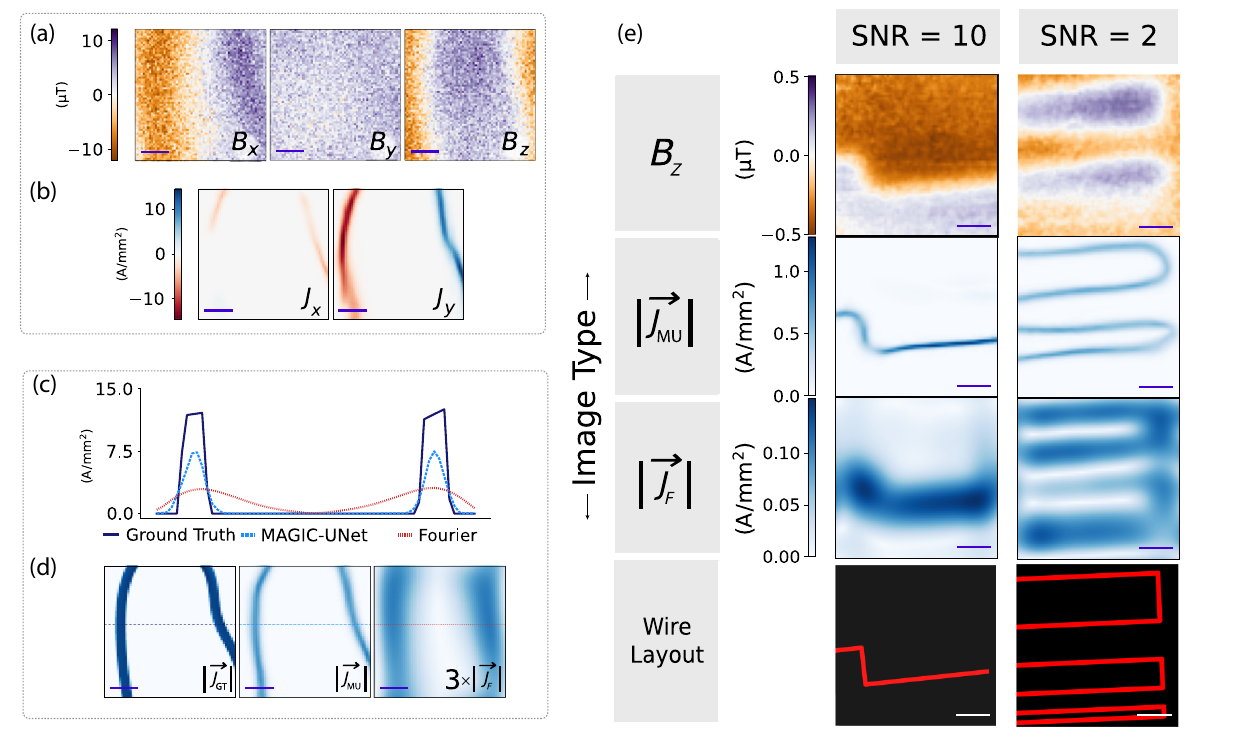
\includegraphics[width=\textwidth]{reed_fig6}
\caption{The large-standoff network, trained at $500\pm50$\um. (a) Synthetic field at 500\um, $\sigma_n = 0.2$. (b)
MAGIC-UNet's $J_x$, $J_y$. (c) A line cut: truth (dark), MAGIC-UNet (blue), Fourier method (red). (d) Current
magnitude: truth, MAGIC-UNet, and three times the Fourier method. (e) Real QDM data at about 500\um, at SNR 10 and 2.
\emph{Source:} Reed et al., Phys.\ Rev.\ Applied \textbf{23}, 034035 (2025), Fig.~6, CC BY 4.0; cropped, otherwise
unchanged.}
\label{fig:reed_fig6}
\end{figure}

A separate $64\times64$ network was trained at $500\pm50$\um, about 5 to 10 times the size of the current features
(Sec.~III~C). There, the paper reports that \emph{both} methods do too poorly for its quantitative scores to mean
anything, and gives no SSIM. Qualitatively MAGIC-UNet is better: wires of roughly the right width in roughly the right
place, where the Fourier method gives a blur. But it has more artefacts than at 50\um, rounded corners, and in the line
cut of Fig.~6(c) its peak current is clearly below the truth.

\begin{careful}[Which of their regimes our tiles are in (ours)]
The field of view is 2\,mm in both of the paper's models (Table~V). So its main model's tile is $2000/50 = 40$
standoffs wide, and its large-standoff model's tile is $2000/500 = 4$. Our run 2 tile is $12.8/3 \approx 4.3$ standoffs
wide; our 10\um\ runs are at $44.8/10 \approx 4.5$. By the pixel count of the earlier table too, $z/\Delta \approx 15$ for
us and 16 for their large-standoff model.

The paper itself defines its large-standoff case by a third ratio, standoff over feature size, ``about 5 to 10 times''
(Sec.~III~C). Our simulator draws wire widths of 1.6--3.2\um\ (\code{simulate_fields.py}), so run 2 is at
$3/3.2$ to $3/1.6$, about 1--2 times, which is nearer their 50\um\ model (50\um\ over widths of 9--320\um, Table~V).
Our 10\um\ runs are at about 3--6 times, near their large-standoff case.

So on tile size and pixels, the paper \emph{did} test our regime, and found its network qualitatively better than
Fourier but not good enough to score. Most of the field in each tile comes from wires outside it. Our results in Chapter~\ref{ch:magic_results} are
measurements in that harder regime, not repeats of the 50\um\ result.
\end{careful}

\section{Four sources, and which one we follow}\label{sec:magic_sources}

That is the paper. The exact architecture needed some detective work, because the sources disagree.
\begin{enumerate}
\item \textbf{The paper} gives the design (Sec.~II, Fig.~1) and the training recipe (Table~IV, Appendix~A).
\item \textbf{The released trained model} (Harvard Dataverse, doi:10.7910/DVN/SD6PVP, the paper's ref.~[61]) contains the
full layer graph. It settles details the text leaves open: pooling stride 2 (the text of Sec.~II says 1), nearest-neighbour
upsampling followed by a $3\times3$ conv without BatchNorm, the order of concatenation, and the initialisation. It also
differs from the text on the decoder: Sec.~II describes an upsampling convolution, then three conv--BatchNorm--ReLU
blocks after the concatenation (four convolutions); the released model has the upsampling conv, BatchNorm and ReLU, then
two blocks (three convolutions). Fig.~1b draws the last, 64-channel level the released way (purple BatchNorm--ReLU, two
blocks, two red convs) and the 256- and 128-channel levels with three yellow blocks. Where they disagree we follow the
released model, because its parameters match the published checkpoint. It has 15,505,194 trainable parameters.
\item \textbf{The released training code} does \emph{not} match either: a different U-Net with tanh and no BatchNorm, a
learning rate of $10^{-5}$, 25 epochs and batch 16. It looks like an older version, so we ignored it.
\item \textbf{Our adaptations}, listed below, each labelled as ours.
\end{enumerate}
So the architecture comes from the released model, and the training recipe from the paper.

\section{Our code}

Each decoder level upsamples, applies a $3\times3$ conv, joins the encoder's skip, then normalises and applies two more
blocks:

\begin{code*}{magic_unet.py}
    def forward(self, x, skip=None):
        x = self.conv(self.up(x))
        if self.skip:
            x = torch.cat([skip, x], dim=1)     # Keras order: [encoder, upsampled]
        return self.blocks(self.norm(x))
\end{code*}

The whole network: three encoder levels, the bottom, and the two decoders fed by the 128- and 256-channel skips (the
64-channel skip is left out, as in Fig.~1b):

\begin{code*}{magic_unet.py}
    def forward(self, b):
        s1 = self.enc1(b)
        s2 = self.enc2(self.pool(s1))
        s3 = self.enc3(self.pool(s2))
        bottom = self.bottom(self.pool(s3))
        return torch.cat([self.jx(bottom, s2, s3), self.jy(bottom, s2, s3)], dim=1)
\end{code*}

\begin{keyidea}[How we know it is exact]
The test file compares every convolution, BatchNorm, pooling, upsampling and concatenation with the layer graph saved
from the released model, in \code{tests/data/magic_unet_released_layers.json}. The parameter count is exactly
15,505,194, and the size of all weights matches the released checkpoint to 0.15\%.
\end{keyidea}

\section{Scaling each image}

The paper divides each image by its own $\alpha_i$ but does not say which number $\alpha_i$ is (Appendix~A). We take the
largest field magnitude in the image, $\alpha = \max|\bm B|$. That is our choice. It is the same quantity the paper uses
to define $\sigma_n$ in Eq.~\eqref{eq:magic_sigma_n}, so the network always sees values up to 1, and a noise of $\sigma$
becomes $\sigma/\alpha$ after scaling, exactly the paper's $\sigma_n$. The output is multiplied back by $\alpha/\beta$:

\begin{code*}{magic_unet.py}
def alpha(b):
    """Per-image scale alpha (Reed et al. App. A; the paper does not name it, we use max over pixels of |B|). b: [..., 3, H, W]."""
    return b.pow(2).sum(-3).sqrt().amax((-2, -1))
\end{code*}

\begin{code*}{train_magic_unet.py}
    a = alpha(b).clamp_min(1e-30)
    x = b / a[:, None, None, None]
    x = x + (sigma / a)[:, None, None, None] * unit_noise(x.shape, generator, corr_um)
    y = j / a[:, None, None, None] * beta
\end{code*}

The noise is added after scaling, with strength $\sigma/\alpha$. Keep that line in mind: it caused the bug in
Chapter~\ref{ch:magic_results}.

\section{From current back to the field}

Our goal is the field at 0.5\um, not the current. The paper stops at the current. But predicting the current is the
better route: once you have the current, Eq.~\eqref{eq:magic_decay} gives the field at \emph{any} height. We use the
thin-sheet Biot--Savart law in Fourier space, in the component frame our simulator shares with COMSOL:

\begin{code*}{magic_unet.py}
    fx, fy = np.fft.rfft2(jx), np.fft.rfft2(jy)
    fz = 1j * (wy * fx - wx * fy) / safe
    decay = 0.5 * MU0_UT * np.exp(-k * height)
    return [np.fft.irfft2(f * decay, s=(ny, nx)) for f in (fx, fy, fz)]
\end{code*}

The factor $\tfrac12\mu_0 e^{-k\cdot\text{height}}$ is Eq.~\eqref{eq:magic_decay}. Going from the current to the field at
0.5\um\ is safe: the factor $e^{-k\cdot0.5\,\mu\text{m}}$ is never larger than 1, so nothing is amplified. The hard part,
undoing $e^{-k\cdot3\,\mu\text{m}}$, is the network's job. The network never needs to know the
0.5\um\ target. It predicts the current, and the physics step does the rest.

\section{Our adaptations}

\begin{center}
\small
\begin{tabularx}{\textwidth}{>{\raggedright\arraybackslash}p{4.3cm}X}
\toprule
Ours & Why \\
\midrule
Our current-layout simulator (spirals, meanders, mirrored arrays) & Their currents come from COMSOL and MATLAB
finite-element runs on random wires (Sec.~V~A), which we cannot reproduce. Ours match the COMSOL test coils. Each layout
gets a random quarter turn and mirror, which gives their 8 augmentations physically. \\
Standoff $3\pm0.6$\um, cut at $\pm3\sigma$ (1.2--4.8\um) & The same 20\% spread as their $50\pm10$\um\ (Table~V),
centred on our benchmark. Never given to the network, as in the paper (Sec.~III). \\
0.2\um\ pixels, $64\times64$ tiles (12.8\um) & Their image size. Simulated at 0.1\um, then averaged $2\times2$, like camera
binning. Tile about 4 standoffs wide, like their 500\um\ model, not their 50\um\ one (Section~\ref{sec:magic_limits}). \\
Target: the equivalent sheet current $J_\text{eff}=J\,e^{-kd}$ & Our wires sit an unknown 0--0.2\um\ below the reference
plane. $J_\text{eff}$ makes the field at every height exact. \\
$\alpha = \max|\bm B|$ & The paper does not say which scalar (Appendix~A); this one matches its $\sigma_n$. \\
White noise at the simulator's 1--2.5\% & The paper does not give its training noise level. Never taken from COMSOL. \\
$\beta = 0.1$ & Their $\beta\approx10^8$ (Appendix~A) is for SI units; ours are \textmu T and A/m. \\
Field from current by Biot--Savart at 0.5\um & The paper stops at the current. \\
Tile overlap chosen from strides 16, 32 and 48 & The paper does not state it. Chosen on simulated images, never on
COMSOL. \\
PyTorch, RMSprop with Keras defaults & Same optimiser maths as their TensorFlow 2.10 version (Table~IV). \\
\bottomrule
\end{tabularx}
\end{center}

\section{The pipeline floor}

Cutting the image into tiles and predicting a current costs something even when the network is perfect, because currents
outside the image are missing. We measured this with the \emph{true} current on simulated layouts:

\begin{center}
\begin{tabular}{lc}
\toprule
Setup, perfect current & Error at 0.5\um \\
\midrule
True current, assuming the mean offset 0.1\um & 5.14\% \\
$J_\text{eff}$ on the full canvas & 0.00\% \\
$J_\text{eff}$ cropped to the image, 0.1\um\ pixels & 2.85\% \\
$J_\text{eff}$ cropped, 0.2\um\ pixels (\textbf{used}) & 2.93\% \\
\bottomrule
\end{tabular}
\end{center}

The field-to-field methods (FISTA, CSC-LISTA, FISTA-Net) do not pay this 2.9\%; MAGIC-UNet does.

\begin{careful}[An honest correction]
At first I blamed the 0.2\um\ pixels for a 7.3\% floor. That was wrong. The real cause was forcing the cropped current to
be divergence-free, which spreads the crop's error over the whole image. Plain Biot--Savart is linear, so the cropped
current costs only the field of the missing outside currents. With that fix the floor is 2.9\%, and the pixel size barely
matters.
\end{careful}

\begin{defend}[If your professor asks: did you change the network?]
No. Every layer matches the authors' released model, checked by tests, with 15,505,194 parameters. The training recipe is
the paper's (Table~IV). What we changed is the data and the scale, each listed as our adaptation, and the step from
current back to field, which the paper does not have.
\end{defend}

\begin{defend}[If your professor asks: isn't ``no standoff needed'' your contribution?]
No. The paper already trains over $50\pm10$\um\ and never tells the network the standoff (Sec.~III, Table~V). What we add
is: running it with tiles about 4 standoffs wide, the tile size at which the paper could not score its own large-standoff
model (Sec.~III~C); going
from the current back to the field at 0.5\um; reading the standoff back out of the predicted current
(Chapter~\ref{ch:height}); and the data-consistency step (Chapter~\ref{ch:consistency}).
\end{defend}

\chapter{MAGIC-UNet results}\label{ch:magic_results}

All MAGIC-UNet runs ran on the server's RTX A6000. Each one generated its own training crops (about 1.7 hours with 24
workers), trained for 50 epochs (about 4 hours, 286 seconds per epoch), then scored itself on simulated images and on every
COMSOL pair. No COMSOL number was used to choose anything.

\section{Run 1: a bug, not a result}

Run 1 trained smoothly, but its scores were terrible: 74\% on simulated images and 82\% on COMSOL at 3\um\ to 0.5\um,
no better than copying the blurry input (75\%). The predicted field was about 3.5 times too small.

The weights were fine. The fault was in BatchNorm. During training, each BatchNorm layer normalises with the statistics of
the current batch, and it also keeps a running average of those statistics to use at test time. We compared the two on
2,048 validation crops:

\begin{center}
\begin{tabular}{lcc}
\toprule
Validation crops, run 1 weights & Current error & Best-fit scale \\
\midrule
Stored running statistics (what was scored) & 93.8\% & 5.8 \\
Statistics of each batch & 17.0\% & 1.00 \\
Running statistics recomputed on clean training batches & 16.8\% & 1.00 \\
\bottomrule
\end{tabular}
\end{center}

The cause was our noise. Run 1 set each layout's noise level from the field range of the \emph{whole} 140\um\ layout.
About 0.5\% of crops lie far from every wire, where the field is tiny. Their noise was therefore huge compared with
their own field, up to 165 times their largest value. Because every crop is divided by its own $\alpha$, those few crops
became enormous noise images, and they corrupted the running variance. Recomputing the statistics with those crops
included gave 98.9\%; without them, 16.8\%.

\begin{figure}[H]
\centering
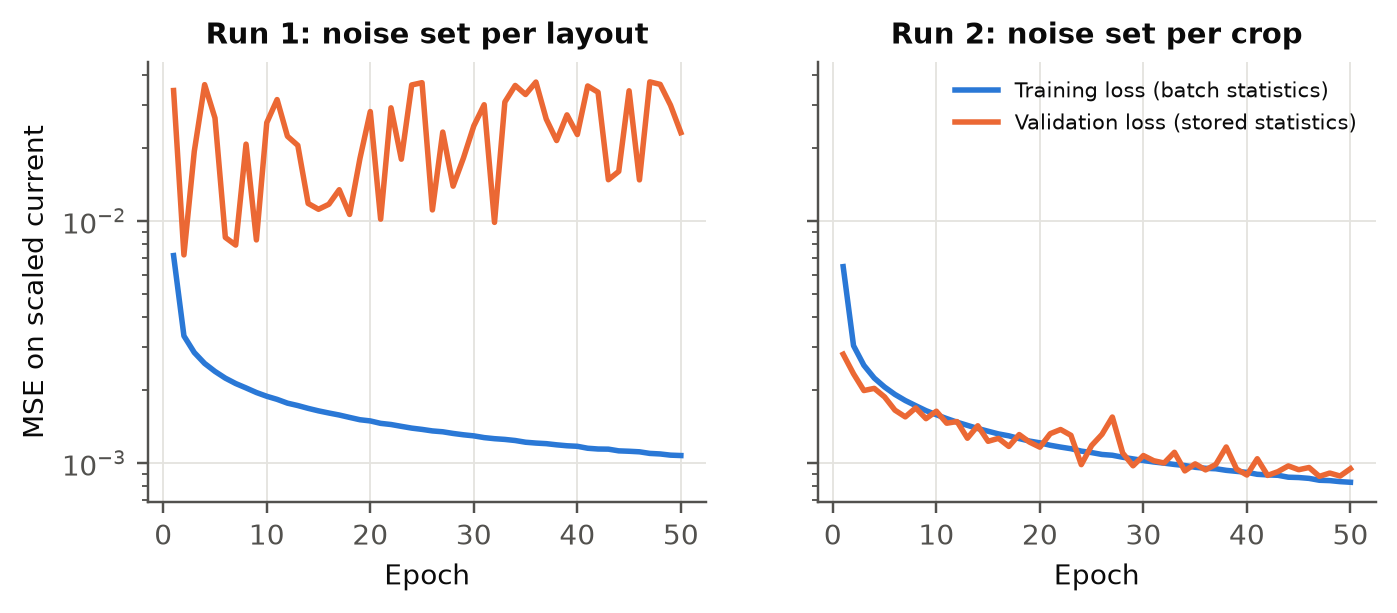
\includegraphics[width=\textwidth]{magic_history}
\caption{Training (blue) and validation (orange) loss. In run 1 the validation loss jumps around and never improves,
because it uses the corrupted stored statistics. In run 2 the two curves follow each other.}
\label{fig:magic_history}
\end{figure}

\begin{careful}[Whose mistake]
This was a flaw in our data design, not in the paper. The paper sets the noise relative to each image's own largest
field. We had copied our simulator's habit of setting it per layout.
\end{careful}

\section{Run 2: the fix}

Run 2 sets the noise from each crop's own field range, as the paper does:

\begin{code*}{magic_data.py}
def crop_sigma(b, percent):
    """White-noise sigma (uT) of one crop b [3, H, W]: percent of its own mean component range."""
    return percent / 100 * float(np.mean(b.max((1, 2)) - b.min((1, 2))))
\end{code*}

The stored crops had no noise in them yet, so they were kept, and a new \code{--resigma} option rewrote only the noise
levels. Run 1 had not saved each crop's percentage, so it was drawn again from the same 1, 1.5, 2 and 2.5\%. Over 20,000
training crops the noise is now at most 4.2\% of a crop's largest field, with a median of 1.4\%.

\begin{careful}
Run 2 is not a pure rerun. Its typical noise is lower than run 1's (1.4\% against 3.0\% of a crop's field), because noise
is no longer inflated far from the wires. Noise level is a setting we chose.
\end{careful}

\subsection{Simulated images}

On 50 full simulated validation images the field error at 0.5\um\ is 15.2\%. The predicted current scores SSIM 0.81 and
0.89 for $J_x$ and $J_y$. Tile stride 32 was chosen here. This number is not comparable with the 48.8\% of
Chapter~\ref{ch:results}, which was scored on 64 signal-rich crops.

\subsection{COMSOL at 3\um\ to 0.5\um}

The score is the same as for every other method: relative $L_2$ per component over the full image, averaged over the same
15 pairs. We checked both scoring paths in the code.

\begin{center}
\small
\begin{tabular}{lcccccccc}
\toprule
Method & Standoff given? & L1\_C1 & IC\_4um & C1+C2 & C1--C3 & C1--C4 & Mean \\
\midrule
\textbf{MAGIC-UNet, run 2} & \textbf{No} & \textbf{26.3\%} & 29.6\% & \textbf{26.6\%} & \textbf{26.4\%} & \textbf{26.0\%} &
\textbf{27.0\%} \\
FISTA-300, $\lambda=0.009$ & Yes & 31.2\% & \textbf{27.6\%} & 31.4\% & 31.2\% & 31.1\% & 30.5\% \\
FISTA-Net, run 2 & Yes & 33.1\% & 34.6\% & 33.2\% & 33.1\% & 32.7\% & 33.3\% \\
\bottomrule
\end{tabular}
\end{center}

\begin{figure}[H]
\centering
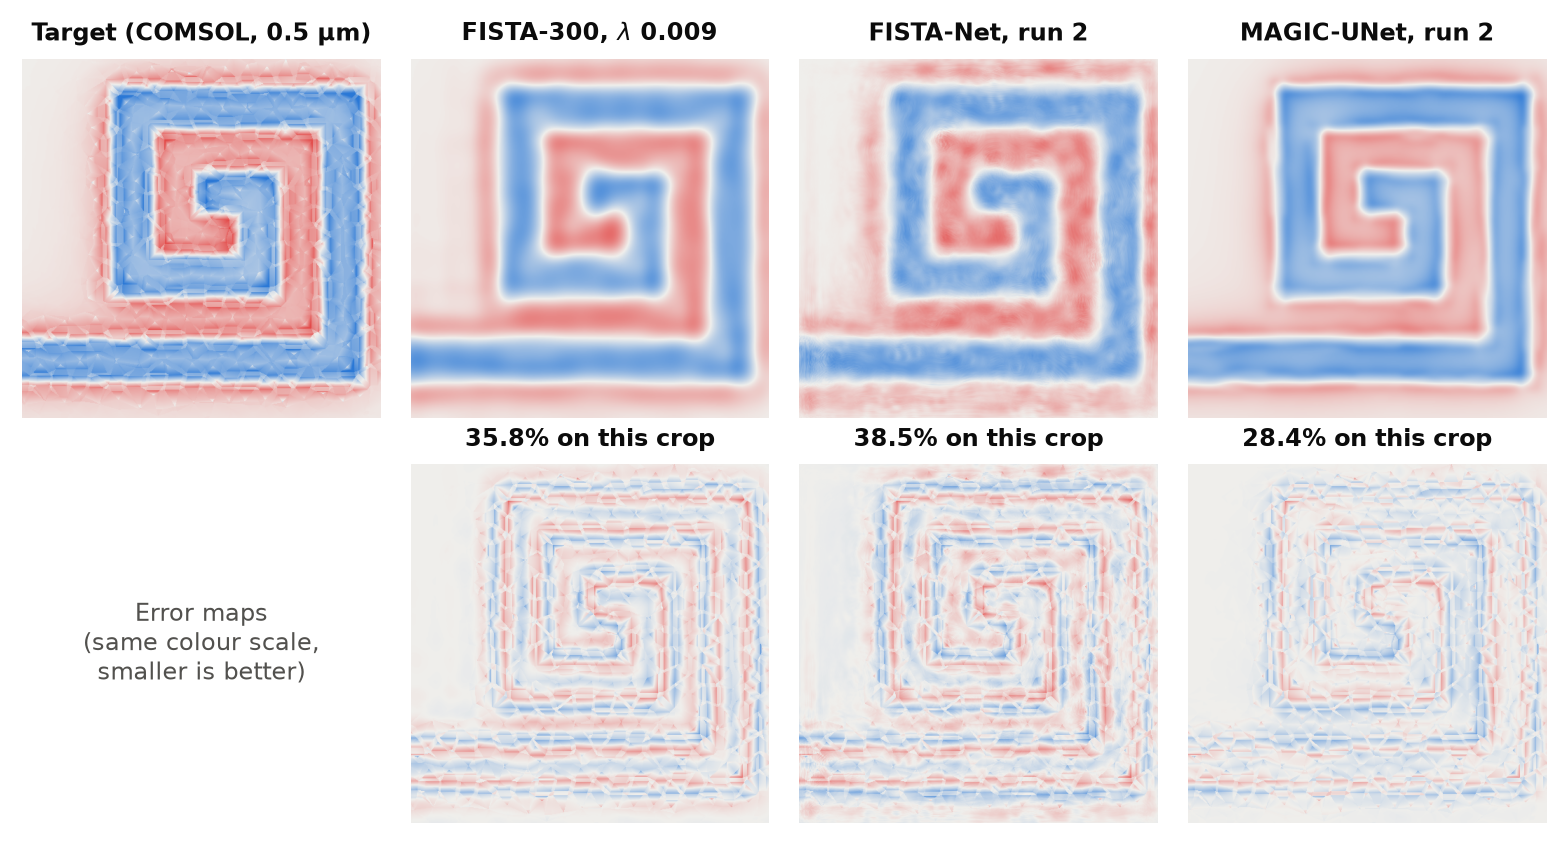
\includegraphics[width=\textwidth]{magic_reconstruction}
\caption{$B_z$ of L1\_C1 at 0.5\um, the same $512\times512$ crop as Chapter~\ref{ch:results}. MAGIC-UNet ran on the full
image and was then cropped; FISTA-300 and FISTA-Net ran on the crop alone, so MAGIC-UNet had more surrounding context.}
\label{fig:magic_reconstruction}
\end{figure}

The maps show the difference: the wire edges are cleaner, and the error maps are fainter along the wires. No tile seams
are visible.

\subsection{Other standoffs}

The same network, never told the height, was scored on every other COMSOL pair. Trained heights were 1.2 to 4.8\um.

\begin{center}
\small
\begin{tabular}{lcccccccccc}
\toprule
Input height (\textmu m), target 0.5\um & 1 & 2 & 3 & 4 & 5 & 6 & 7 & 8 & 9 & 10 \\
\midrule
Mean error & 59\% & 32\% & 27\% & 37\% & 52\% & 67\% & 78\% & 87\% & 92\% & 94\% \\
Inside the trained range & no & yes & yes & yes & no & no & no & no & no & no \\
\bottomrule
\end{tabular}
\end{center}

IC\_2um at 2\um\ to 1\um\ scores 26.6\%. Most heights have one or two coils, so only the 3\um\ column is a 15-pair score.

\begin{figure}[H]
\centering
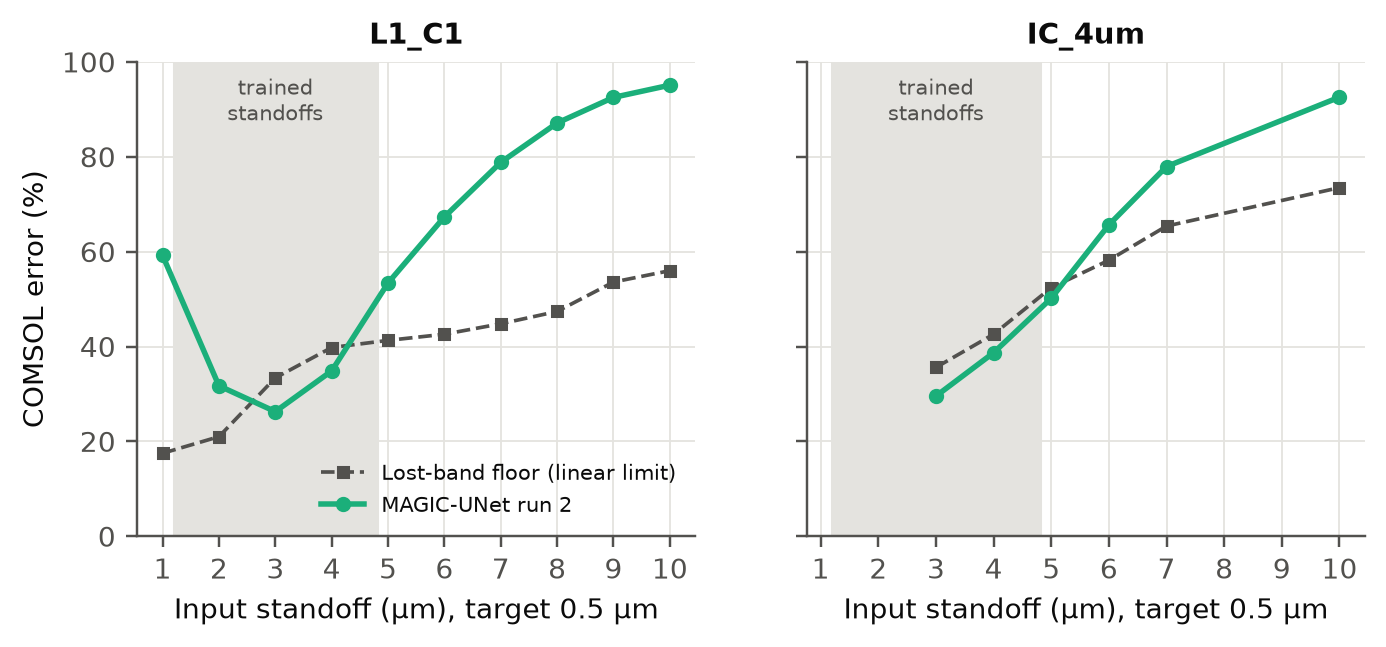
\includegraphics[width=\textwidth]{magic_standoff}
\caption{MAGIC-UNet error against input standoff for each coil, with the lost-band floor of Chapter~\ref{ch:floor}. The
grey band is the range of standoffs seen in training.}
\label{fig:magic_standoff}
\end{figure}

\begin{keyidea}[What run 2 shows]
\begin{itemize}
\item \textbf{Inside the trained range, one network handles an unknown standoff.} At 3\um\ it beats every method that was
given the height. At 3 and 4\um\ on both coils it even goes below the lost-band floor, so its learned prior fills in part
of the lost band. At 2\um\ it stays above the floor.
\item \textbf{Outside the range it fails quickly,} in both directions. At 1\um\ it is far worse than the floor, even though
that input is less blurred than anything it trained on. The network learned to expect a certain amount of blur.
\end{itemize}
\end{keyidea}

\section{Run 3: any standoff}

You asked whether one network could cover every standoff. The architecture needs no change, because the network never sees
the height. Only the training range changes. To keep the comparison explainable, run 3 changes \textbf{exactly one thing}
from run 2:

\begin{center}
\begin{tabular}{lcc}
\toprule
 & Run 2 & Run 3 \\
\midrule
Training standoff & $3\pm0.6$\um, 1.2--4.8\um & uniform over 1--10\um \\
Everything else & \multicolumn{2}{c}{identical: network, $64\times64$ tiles, crops, noise, recipe, scoring} \\
\bottomrule
\end{tabular}
\end{center}

The range 1--10\um\ is exactly the span of the COMSOL inputs. The paper trained one model per standoff range, so a single
1--10\um\ model is our adaptation. Larger tiles were considered for large standoffs and dropped, to stay close to the
paper. Run 3 was launched on 8 November. Its results are in Chapter~\ref{ch:run3}.

\begin{careful}[What to expect from run 3]
At large standoffs most of the target is missing from the data (Chapter~\ref{ch:floor}: 56--73\% at 10\um), so no method will
score well there. The questions are whether 1\um\ and 5--10\um\ improve on run 2, and how much a single any-standoff
network loses at 3\um\ compared with run 2's 27.0\%.
\end{careful}

\section{Is MAGIC-UNet the clear winner?}

Not yet. It is the best result we have, but the claim has limits.
\begin{enumerate}
\item \textbf{Only two geometries.} C2--C4 mirror C1, so the five configurations hold two wire shapes. MAGIC-UNet wins
clearly on the L1/C1 shape (about 26\% against 31\%) and loses on the IC coil (29.6\% against 27.6\%). That is one win and
one loss.
\item \textbf{One training run.} FISTA gives the same answer every time; a trained network does not. Without more seeds we
cannot say how solid a 3.5-point lead is.
\item \textbf{Not like-for-like.} MAGIC-UNet trained on 2,400 layouts and sees all three field components together.
Strict CSC-LISTA and FISTA-Net trained on 200 layouts and see one component at a time. The fair claim is ``MAGIC-UNet, as
we set it up, beats them'', not ``the architecture is better''. Size and data volume alone are unlikely to explain it:
MAGIC-UNet has 15.5 million parameters against 49 million for strict CSC-LISTA at 64 layers (and 75 thousand for
FISTA-Net), and 8,000 layouts made CSC-LISTA worse (Chapter~\ref{ch:followups}).
\item \textbf{No baselines at other standoffs.} Nothing else has been scored at 2 or 4\um\ yet.
\item \textbf{Only what we tried.} Diffusion priors and the untrained network of Dubois et al.\ have not been tested.
\item \textbf{The research question asks for more.} MAGIC-UNet reconstructs well without the height, but it does not
estimate the height or say how sure it is.
\end{enumerate}

\begin{keyidea}[The fair summary]
MAGIC-UNet is the best reconstruction method we have tested at 3\um\ to 0.5\um, and the first that does not need the
standoff. Its lead holds on one of the two coil shapes. It is a strong reconstruction baseline, not yet the complete method
the research question asks for.
\end{keyidea}

\section{What would settle it}

\begin{enumerate}
\item \textbf{FISTA-300 at 2 and 4\um}, once given the true height and once assuming 3\um. This is the baseline for the
unknown-standoff claim, and it takes under an hour.
\item \textbf{Two more seeds of MAGIC-UNet run 2}, about 4 hours each, to see whether 27.0\% holds.
\item \textbf{Run 3's results}, for one network across all standoffs.
\item \textbf{The identifiability check} of Chapter~\ref{ch:question}, before any joint height estimation.
\end{enumerate}

\begin{defend}[If your professor asks: is this just a bigger network winning?]
Not simply. MAGIC-UNet has 15.5 million parameters, fewer than strict CSC-LISTA at 64 layers (49 million), which it beats.
Giving CSC-LISTA forty times more layouts made it worse, so more data alone is not the explanation either. The network is
unmodified from the paper, it never saw COMSOL, and it was not told the standoff, while every method it beats was. It does
see all three components at once, which the others do not, and that may help.
\end{defend}

\begin{defend}[If your professor asks: does it solve the unknown-standoff problem?]
Inside its training range, partly: one network reconstructs at 2, 3 and 4\um\ without being told which. Outside that range
it fails, and it never outputs a height or an uncertainty. Run 3 tests the first point; the second needs the methods in
Chapter~\ref{ch:question}.
\end{defend}

\begin{careful}[Since this chapter was written]
All four steps above were done between 9 and 12 November. They changed the picture: FISTA had been stopped too early,
and the lead of MAGIC-UNet now rests on one added correction step. Read Chapters~\ref{ch:run3} to~\ref{ch:consistency} before
quoting any number from this chapter. Chapter~\ref{ch:ten} takes the method to 10\um.
\end{careful}

\section{What is not yet known}

\begin{itemize}
\item How much MAGIC-UNet's score varies between seeds.
\item Whether its lead holds on a third wire shape. Today it wins on one shape and loses on the other.
\item How FISTA and the other methods do at 2 and 4\um, with and without the true height.
\item Whether one network can cover 1--10\um\ (run 3).
\item Whether any source prior makes the height identifiable on COMSOL.
\item Everything on experimental QDM data. Nothing here has been tested on real measurements.
\end{itemize}

\chapter{Run 3: one network for every standoff}\label{ch:run3}

Chapters~\ref{ch:floor} to~\ref{ch:magic_results} end on 8 November, with run 3 still training. This chapter and the
eight after it cover 8 to 16 November. They are written the same way as the rest: every idea is rebuilt from the
start, and every grey block is copied from the repository.

\section{What run 3 changes}

Run 2 was trained on standoffs of $3\pm0.6$\um. You asked whether one network could cover \emph{any} standoff. The
network never sees the height, so the architecture needs no change. Only one line of the data generator differs: how
the standoff of each training crop is drawn.

\begin{code*}{magic_data.py}
        if cfg.get('z_uniform'):                  # run 3: any standoff in [lo, hi]
            zs.append(float(rng.uniform(*cfg['z_uniform'])))
            continue
        z = rng.normal(cfg['z_mean'], cfg['z_std'])
        if abs(z - cfg['z_mean']) <= cfg['z_trunc'] * cfg['z_std']:
            zs.append(float(z))
\end{code*}

Run 2 takes the bottom three lines: a normal distribution around 3\um, cut at three standard deviations. Run 3 takes the
top branch with \code{--z-uniform 1 10}: every height from 1 to 10\um\ is equally likely. Everything else is identical.

\section{The result}

On the simulated validation layouts, with the target always at 0.5\um:

\begin{center}
\small
\begin{tabular}{lcccccccccc}
\toprule
Input standoff (\textmu m) & 1 & 2 & 3 & 4 & 5 & 6 & 7 & 8 & 10 \\
\midrule
Run 2 ($3\pm0.6$\um) & 22.8\% & 14.2\% & 15.1\% & 15.4\% & 25.4\% & 48.1\% & 67.9\% & 80.5\% & 92.0\% \\
Run 3 (1--10\um) & 35.3\% & 26.1\% & 22.7\% & 22.1\% & 26.1\% & 31.2\% & 33.7\% & 36.1\% & 56.8\% \\
\bottomrule
\end{tabular}
\end{center}

And on COMSOL at 3\um\ to 0.5\um:

\begin{center}
\begin{tabular}{lccc}
\toprule
 & 15 pairs & C1-family coils & \code{IC_4um} \\
\midrule
Run 2 & 27.0\% & 26.3\% & 29.6\% \\
Run 3 & 34.8\% & 30.4\% & 52.0\% \\
\bottomrule
\end{tabular}
\end{center}

\begin{keyidea}[What run 3 shows]
\begin{itemize}
\item \textbf{A wide range has a price.} Inside run 2's range (2--4\um) run 3 is 7 to 12 points worse. A network that must
be ready for any blur is less sure about each one.
\item \textbf{It buys reach.} From 5 to 8\um\ run 3 holds at 26--36\% where run 2 collapses.
\item \textbf{It breaks at the edge of its own range.} At 10\um\ it jumps to 56.8\%. Remember this number: it is the reason
the 10\um\ runs of Chapter~\ref{ch:ten} are trained with 10\um\ in the \emph{middle} of their range.
\end{itemize}
\end{keyidea}

\section{Why the IC coil fails}

On \code{IC_4um} run 3 scores 52\%, and by component it is 31 / 69 / 56\% for $B_x$ / $B_y$ / $B_z$. That is not noise. It has
a cause, and the cause is the ambiguity of Chapter~\ref{ch:question}.

The IC coil has pairs of wires close together that carry current in \emph{opposite} directions. Far above such a pair
the two fields nearly cancel. What survives is weak and smooth. But ``weak and smooth'' is also exactly what a single
wire looks like from far away. So a tile that sees such a pair has two explanations:
\begin{itemize}
\item two opposite wires, close to the sensor; or
\item one source, far from the sensor, which must then be made much stronger and sharper to explain the same field.
\end{itemize}
Run 2 only knows heights near 3\um, so it has no choice but the first. Run 3 was told that anything from 1 to 10\um\ is
possible, and on these tiles it picks ``far''. It then over-amplifies, and the 0.5\um\ field comes out wrong.

There is a second ingredient. MAGIC-UNet works tile by tile, and each $12.8$\um\ tile makes this decision \emph{alone}.
Nothing tells neighbouring tiles that the whole image was measured at one height.

\begin{careful}[What is established and what is not]
The pattern (the failure sits on the closely spaced opposite wires, and different tiles imply different heights) was
measured on the server. The explanation is the best one we have, and Chapter~\ref{ch:height} tests one consequence of
it: if the only problem were the per-tile height, then forcing \emph{one} height on the whole image should rescue run 3.
It does not.
\end{careful}

\begin{defend}[If your professor asks: so can one network handle an unknown standoff?]
Inside a narrow band, yes: run 2 works from 2 to 4\um\ without being told the height. Across a wide band it works on
simple wires and fails where the wires are ambiguous, because the field alone cannot separate ``close and weak'' from
``far and strong''. That is the height ambiguity showing up inside a trained network.
\end{defend}

\chapter{The review: what the benchmark can and cannot say}\label{ch:review}

On 10 November the whole project was reviewed critically: every document, script, test and saved run. The result is
\code{FABLE_REVIEW.md}, about 800 lines. This chapter teaches what is in it, because it changed how every number in
this booklet should be read. The next four chapters are the experiments that the review asked for.

\section{How the review was done}

Nothing was trained. The review read the files, and it ran small NumPy checks on the saved predictions
(\code{scripts/review_checks.py}, about two minutes). Every statement carries a tag that says how far to trust it:
\begin{itemize}
\item \textbf{[file]}: a number read from a repository file or a saved run.
\item \textbf{[check]}: a number the review computed itself from saved arrays. These used the two COMSOL configurations
that are on the Mac, so they are diagnostics on test data, not results.
\item \textbf{[web]} and \textbf{[memory]}: a reference found by a search, or known but not fetched again.
\item \textbf{[not verified]}: stated in our documents, and not confirmed.
\end{itemize}

\section{The verdict}

\begin{keyidea}[The review in three sentences]
The project asks the right question, and its last move, a network that works in the current domain, was the right one.
But most of the effort had gone into ranking field-domain networks by 1 to 3 points on a benchmark that cannot support
such rankings. The benchmark has two wire shapes, one seed per method, a noisy target and an unexplained physics
anomaly, and it had been used to compare more than twenty method variants.
\end{keyidea}

\section{What went right}

It is worth knowing these too, because they are what you can defend without hesitation.
\begin{itemize}
\item \textbf{Test hygiene.} Since the restart, COMSOL is kept out of training, normalisation and model selection, and
the code enforces it.
\item \textbf{Faithful baselines.} The MAGIC-UNet port is checked layer by layer against the released model, and the
run 1 failure was diagnosed, not tuned away.
\item \textbf{Asking for the limit.} The Wiener oracle and the lost-band floor (Chapter~\ref{ch:floor}) are the right kind
of question.
\item \textbf{The ambiguity analysis} of Chapter~\ref{ch:question} is correct, and it is the core of a possible paper.
\item \textbf{The run 3 diagnosis} is a real finding, not a bug report.
\end{itemize}

\section{What the ``15 pairs'' really are}

Every score in this booklet is a mean over ``15 COMSOL pairs''. Look at what they are:

\begin{center}
\small
\begin{tabularx}{\textwidth}{>{\raggedright\arraybackslash}p{4.4cm}X}
\toprule
What it looks like & What it is \\
\midrule
15 test images & 5 coil configurations $\times$ 3 field components \\
5 configurations & 2 wire shapes. \code{C1_C2}, \code{C1_C2_C3} and \code{C1_C2_C3_C4} are mirror copies of
\code{L1_C1} (correlation 0.97--0.98) \\
Independent noise in each & The same mesh noise: all four C1 configurations come from one COMSOL solve \\
Unseen data & The simulator was built around these coils: its layout families, wire widths, current and noise level
all come from them \\
One look per method & At least 22 method variants scored on the same 15 pairs. FISTA's $\lambda$ was retuned after
network scores were known; FISTA-Net got a second run because of its first COMSOL score \\
\bottomrule
\end{tabularx}
\end{center}

\begin{careful}[What follows from this table]
Each step was defensible on its own. Together they mean two things. First, the test set measures performance on the two
shapes the simulator was designed for, not on new geometries. Second, when many variants are tried on one small test
set, the best one looks better than it is. A difference of 1 to 3 points, on one seed, is not a finding.
\end{careful}

\section{What went wrong, sorted by cause}

The review sorts the problems into five kinds. This is the useful part: it tells you \emph{which kind} of fix each one
needs.

\textbf{(a) Information limits.} Part of the 0.5\um\ field is simply not in the 3\um\ measurement. This is real, but the
``floor'' of 34.5\% in Chapter~\ref{ch:floor} overstates it, because it mixes two different things: real field that was
lost, and mesh noise in the target that no method could ever reproduce. Chapter~\ref{ch:limits} separates them.

\textbf{(b) Modelling errors.} The blur model $e^{-k\,\Delta z}$ is physics, but COMSOL does not follow it exactly. At
3\um\ the mismatch is 10--17\%. At 10\um\ it is 64--140\%, more than any real field could decay. Chapter~\ref{ch:comsol}
finds out why. COMSOL's three components are also not consistent with each other, and MAGIC-UNet's two outputs $J_x$ and
$J_y$ come from separate decoders, so its current does not conserve charge exactly.

\textbf{(c) Data problems.} Two test shapes, shared mesh noise, a simulator built around them, no sensor noise anywhere,
and no real measurement.

\textbf{(d) Optimisation and architecture.}
\begin{itemize}
\item \emph{CSC-LISTA is under-trained, not data-limited.} At 64 layers it has 49 million parameters, trains for 1{,}000
steps and keeps the checkpoint from step 100--300. On its \emph{own} training distribution it loses to plain FISTA at the
same depth with the same dictionary (48.8\% against 45.3\% at 64). A learned network that cannot beat the method it
starts from has an optimisation problem.
\item \emph{It is not doing sparse coding.} 99\% of its code values are non-zero. With dense codes it behaves almost like a
linear filter, which is why it ends up next to the best linear filter (Chapter~\ref{ch:floor}).
\item \emph{FISTA-300 is not converged.} Its error was still falling from 32 to 64 to 300 iterations, and nobody had run
1{,}000. Chapter~\ref{ch:fista_depth}.
\item \emph{MAGIC-UNet has no data-consistency step and a small view.} Nothing forces its output to agree with the
measurement, and its 12.8\um\ tile is only about four standoffs wide. Chapters~\ref{ch:consistency} and~\ref{ch:ten}.
\end{itemize}

\textbf{(e) Evaluation.} The metric is taken against a noisy target, with one seed and no error bars, and models are
selected on 64 crops.

\section{The surprising results, one by one}

For each result that had seemed strange, the review gives the explanation that the evidence supports best, and a cheap
test that could prove that explanation wrong. Most of these tests were then run.

\begin{center}
\small
\begin{tabularx}{\textwidth}{>{\raggedright\arraybackslash}p{3.3cm}>{\raggedright\arraybackslash}X>{\raggedright\arraybackslash}p{4.6cm}}
\toprule
Result & Best-supported explanation & What the test then showed \\
\midrule
CSC-LISTA got worse with 8{,}000 layouts (33.8 to 36.0\%) & Checkpoint and seed noise. Both runs kept a checkpoint from
step 100--200, before the extra layouts could matter & Not run. The claim ``data volume is not the limit'' of
Chapter~\ref{ch:followups} is not supported \\
Learned field-domain networks sit next to the Wiener oracle & With dense codes they act almost linearly, so they can only
restore the measured band & Holds: they leave 79--82\% of the next band unrecovered (Chapter~\ref{ch:limits}) \\
FISTA-300 beats every learned field-domain network & FISTA was still improving at 300 iterations; the networks stop at 64
layers & FISTA is best at 1{,}000 iterations: 26.7\%, not 30.5\% (Chapter~\ref{ch:fista_depth}) \\
MAGIC-UNet beats methods that were given the standoff & Its current-domain prior fills in frequencies just above what
the measurement carries & Against FISTA-1000 the raw network only ties; with one correction it wins
(Chapter~\ref{ch:consistency}) \\
Run 3 fails on the IC coil & Each tile decides its own height & One global height does not rescue it: 52.0 to 46.9\%
(Chapter~\ref{ch:height}) \\
\bottomrule
\end{tabularx}
\end{center}

\begin{keyidea}[Notice the last row]
The review's own prediction was wrong there, and the document says so. A good review states its explanations in a
form that an experiment can refute, and then reports the refutation.
\end{keyidea}

\section{Corrections to earlier chapters of this booklet}

\begin{careful}[Read these before quoting Chapters 9 to 19]
\begin{itemize}
\item \textbf{Chapter~\ref{ch:floor}:} ``any method below 34.5\% must be filling in lost frequencies'' is too strong. The
floor is inflated by noise in the target. See Chapter~\ref{ch:limits}.
\item \textbf{Chapter~\ref{ch:followups}:} ``data volume is not what limits CSC-LISTA'' and ``the limit is the simulator
gap'' are not supported by that experiment.
\item \textbf{Chapter~\ref{ch:defence}:} ``$h$ stays fixed because it is physics and we know it exactly'' is true of physics.
It is not true of this COMSOL export, which does not obey free-space physics (Chapter~\ref{ch:comsol}).
\item \textbf{Chapter~\ref{ch:question}:} ``the height cannot come from the field alone'' is right, but the ambiguity is
\emph{one-sided}. Without any prior the data still give an upper bound on the depth (Chapter~\ref{ch:limits}).
\item \textbf{Chapters~\ref{ch:results} to~\ref{ch:magic_results}:} every comparison with ``FISTA'' there means FISTA at 300
iterations, which was stopped too early.
\end{itemize}
\end{careful}

\section{What the review said to stop, and to do}

\textbf{Stop:} new CSC-LISTA, LFISTA and FISTA-Net variants; reading differences under about 3 points; reporting
5--10\um\ COMSOL scores as physics before the decay anomaly is explained; treating $B_x$, $B_y$ and $B_z$ as three
unrelated images; quoting the lost-band floor as a limit of the problem.

\textbf{Do}, as a list of milestones:

\begin{center}
\small
\begin{tabularx}{\textwidth}{l>{\raggedright\arraybackslash}X>{\raggedright\arraybackslash}p{4.2cm}}
\toprule
 & Milestone & Status on 16 November \\
\midrule
M1 & Re-score run 2 and run 3 with a data-consistency step and a height read-out. No training & Done:
Chapters~\ref{ch:height} and~\ref{ch:consistency} \\
M2 & Repair the measuring stick: noise edge, scores by band, FISTA run longer, more seeds & Done:
Chapters~\ref{ch:limits}, \ref{ch:fista_depth}, \ref{ch:consistency} \\
M3 & Open the COMSOL model and explain the fast decay; export new geometries & First half done:
Chapter~\ref{ch:comsol}. No new geometries \\
M4 & Classical test of whether the height can be identified & Not done \\
M5--M6 & A new solver: learned current prior inside data-consistency steps, with a search over height & Not done \\
M7--M9 & Generalisation tests, real QDM data, uncertainty & Not done \\
\bottomrule
\end{tabularx}
\end{center}

What the review recommends building after these milestones is in Chapter~\ref{ch:next}.

\section{What is already published, and what is left to claim}

The review searched the literature so that you do not claim something that exists.

\textbf{Do not claim as new:} learning the map from field to current (Reed et al.); using all three field components
(Broadway et al.\ 2020); a sparse or total-variation prior on the current; fitting the sensor distance jointly with
the source as an idea (Setescak et al.\ 2026, for magnetisation); unrolled networks that are told the blur (USRNet);
``a network that works without being told the standoff'', \emph{if} Reed et al.\ already trained over $50\pm10$\um.
The review marks that point as not verified, and Chapter~\ref{ch:magic} explains why it is open.

\textbf{Still open, if the experiments deliver:} inferring the standoff for the whole image with a learned current prior
and exact physics; the one-sided analysis of the ambiguity with a measured height resolution; a reconstruction that
states which frequencies came from the data and which from the prior; validation across standoffs and on a real QDM.

\begin{defend}[If your professor asks: was most of the earlier work wasted?]
No, but it was aimed at the wrong target. The unrolled networks taught us where the limit of field-domain methods is,
and the review used their saved outputs to show why. What was wasted was the ranking: differences of a few points
between them were never real.
\end{defend}

\begin{defend}[If your professor asks: how do you know your winner is not just the luckiest of 22 tries?]
You do not, from the old test alone. That is why the next step was a protocol written before any new score
(Chapter~\ref{ch:fista_depth}), three seeds, and a rule fixed in advance for what counts as a win
(Chapter~\ref{ch:consistency}).
\end{defend}

\chapter{The limits of reconstruction, looked at again}\label{ch:limits}

Chapter~\ref{ch:floor} gave one number for the limit: the lost-band floor, 34.5\% at 3\um. The review showed that this
one number hides three different things. This chapter separates them. It is the most important chapter for
understanding what any score in this project means.

\section{Three bands instead of one floor}

Think of the 0.5\um\ field as a sum of ripples, each with a spatial frequency $k$ (in rad/\um). Fine detail is high $k$.
The blur multiplies each ripple by $H(k)=e^{-k\,\Delta z}$, so fine detail is damped most. Sort the ripples into three
bands:

\begin{center}
\small
\begin{tabularx}{\textwidth}{>{\raggedright\arraybackslash}p{2.6cm}>{\raggedright\arraybackslash}p{3.1cm}X}
\toprule
Band & Frequencies & What it is \\
\midrule
\textbf{Measured band} & below $k_c$ & The blurred signal is still stronger than the noise. A method only has to undo
the blur. \\
\textbf{Prior band} & from $k_c$ to $k_n$ & The signal has sunk below the noise in the measurement, but the target there is
real field: wire edges. Only a method that \emph{knows what sources look like} can fill it in. \\
\textbf{Noise band} & above $k_n$ & The target itself is mesh noise here. No method can reproduce it, and none should. \\
\bottomrule
\end{tabularx}
\end{center}

\begin{figure}[H]
\centering
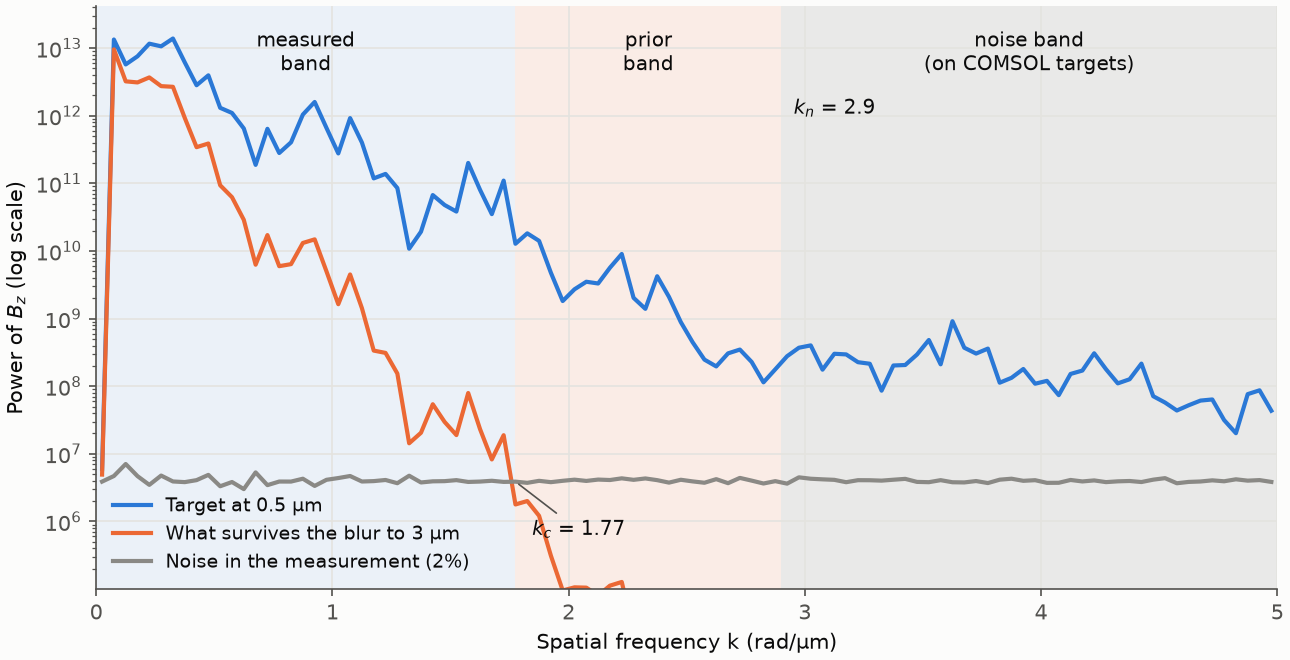
\includegraphics[width=0.88\textwidth]{late_bands}
\caption{The three bands on a simulated layout at 3\um\ to 0.5\um. Blue: power of the target. Orange: what survives the
blur. Grey: the noise level. Where orange drops below grey ($k_c$), the measurement stops carrying information.}
\label{fig:late_bands}
\end{figure}

On the 15 COMSOL pairs, measured as a share of the target's norm:
\begin{center}
\begin{tabular}{lccc}
\toprule
 & Measured band & Prior band & Noise band \\
\midrule
Share of the target's norm & 93.0\% & 32.9\% & 15.7\% \\
\bottomrule
\end{tabular}
\end{center}
These add as squares, not as plain numbers: $93.0^2+32.9^2+15.7^2\approx100^2$. That rule matters, and it comes back
below.

\section{The first edge, $k_c$: where signal sinks below noise}

$k_c$ is the frequency where the blurred signal and the noise are equally strong. The code walks up in steps of
0.05\,rad/\um\ and stops at the first step where the noise wins:

\begin{code*}{m12_common.py}
    h = np.exp(-k * dz)
    sig = np.abs(h * fs) ** 2
    res = np.abs(fb - h * fs) ** 2
    for a in np.arange(0, 8, 0.05):
        m = (k >= a) & (k < a + 0.05)
        if sig[m].sum() < res[m].sum():
            return float(a)
\end{code*}

Here \code{fs} is the spectrum of the sharp target and \code{fb} that of the measured input. \code{sig} is the power the
blur lets through. \code{res} is whatever in the measurement the blur model cannot explain, which is the noise. At
3\um\ on COMSOL, $k_c$ is between 1.0 and 1.6\,rad/\um.

\begin{careful}
$k_c$ uses the true target. So the band split is a way to \emph{diagnose} a method afterwards. It is not something a
method could use while reconstructing.
\end{careful}

\section{The second edge, $k_n$: where the target becomes noise}

How can we tell noise from field in the target, when we have no cleaner target to compare with? With physics. The
three components $B_x$, $B_y$, $B_z$ are not three independent images.

Above the sources there is no current, so the field can be written as the slope of one scalar function,
$\mathbf{B}=-\nabla\Phi$, and that function decays upward as $e^{-kz}$. Take the slope in each direction and the three
components at frequency $(k_x,k_y)$ become
\[
B_x=-i k_x\,\Phi,\qquad B_y=-i k_y\,\Phi,\qquad B_z=k\,\Phi .
\]
\textbf{One number $\Phi$ fixes all three.} In the component frame of our files (COMSOL's export is turned by a quarter
turn, Chapter~\ref{ch:comsol}) the same statement reads
\[
B_x=\frac{k_y}{k}\,\varphi,\qquad B_y=-\frac{k_x}{k}\,\varphi,\qquad B_z=i\,\varphi .
\]
So at each frequency, a real field is one complex number $\varphi$ times the fixed direction
$u=(k_y/k,\;-k_x/k,\;i)$. Mesh noise has no reason to point along $u$. The test is therefore: project the three measured
numbers onto $u$, and call the rest inconsistent.

\begin{code*}{m12_common.py}
    ux, uy, uz = ky / safe, -kx / safe, 1j * np.ones_like(k)
    phi = (np.conj(ux) * spectrum[0] + np.conj(uy) * spectrum[1] + np.conj(uz) * spectrum[2]) / 2
    out = np.stack([ux * phi, uy * phi, uz * phi])
\end{code*}

The division by 2 is the squared length of $u$: $(k_y^2+k_x^2)/k^2+1=2$. So \code{phi} is the least-squares best
$\varphi$, and \code{out} is the part of the field that one current sheet could have produced.

Now sum, in rings of width 0.1\,rad/\um, the total energy and the inconsistent energy of the five 0.5\um\ targets:

\begin{code*}{m12_common.py}
        r = f - sheet_consistent(f, kx, ky, k)
        idx = np.digitize(k, edges) - 1
        ok = (idx >= 0) & (idx < len(total))
        total += np.bincount(idx[ok], (np.abs(f) ** 2).sum(0)[ok], len(total))
        bad += np.bincount(idx[ok], (np.abs(r) ** 2).sum(0)[ok], len(total))
\end{code*}

The rule, fixed before any prediction was scored: $k_n$ is the first ring above 1\,rad/\um\ where more than half of the
energy is inconsistent.

\begin{code*}{m12_common.py}
    frac = bad / np.maximum(total, 1e-300)
    for edge, f in zip(lower, frac):
        if edge >= k_min - 1e-9 and f > share:
            return float(edge)
\end{code*}

\begin{center}
\begin{tabular}{lc}
\toprule
Frequency (rad/\um) & Inconsistent share of the targets' energy \\
\midrule
0.3 to 1.7 & below 3\% \\
1.9 to 2.4 & 14 to 31\% \\
\textbf{2.9} & \textbf{first above 50\%} \\
3 to 12 & 42 to 61\% \\
\bottomrule
\end{tabular}
\end{center}

So $k_n=2.9$\,rad/\um. Why is the share only about a half, and not 100\%, where it is all noise? Because noise is random
in three directions and the test removes two of them. Pure independent noise gives a share of about $2/3$.

\begin{keyidea}[A second, independent confirmation]
Chapter~\ref{ch:comsol} has COMSOL fields of the same coil on two different meshes. Above 2.9\,rad/\um\ they differ from
each other by a factor of 1.4, which is $\sqrt2$: exactly what two independent noise images give. Two unrelated
methods put the edge at the same place.
\end{keyidea}

\begin{careful}[An honest correction]
The review first put the edge at 2.2\,rad/\um, chosen by eye, and wrote that ``18--20\% of every score is mesh noise''.
Both were wrong. The fixed rule gives 2.9. And the noise does not add 16 points to a score, as the next section shows.
\end{careful}

\section{Errors add as squares}

A method's error can be split by band in the same way as the target. The three parts add as squares:
\[
\text{raw}^2=\text{(measured-band error)}^2+\text{(prior-band error)}^2+\text{(noise-band error)}^2 .
\]
Every method outputs nothing sensible in the noise band, so its error there equals the target's own content, about
15.7\%. That is the same for everyone. Removing it:
\[
\sqrt{30.5^2-15.6^2}\approx26.2\%,\qquad \sqrt{24.3^2-15.9^2}\approx18.4\% .
\]
So the noise band lifts a raw score by about 4 to 6 points, not by 15.7. And because it is added in squares to every
method, it \emph{squeezes the differences between methods}. Two methods that are 6 points apart in raw score are 8
points apart once the shared noise is removed.

\section{Scoring four ways}

From here on every method is scored four ways: raw, against the target with the noise band cut off (``low-passed''), in
the measured band alone, and in the prior band alone. All four come from one function. Its core:

\begin{code*}{m12_common.py}
        def band(mask, a):
            return float(np.sqrt((np.abs(a) ** 2)[mask].sum() / n_pix) / norm)
        low = k < k_noise
\end{code*}

\begin{code*}{m12_common.py}
            in_band=band(k < kc, err), prior_band=band((k >= kc) & (k < k_noise), err),
            noise_band=band(k >= k_noise, err), k_c=kc,
\end{code*}

\code{err} is the spectrum of (output minus target). \code{band} keeps only the frequencies in the mask and measures
what is left, as a fraction of the whole target.

\begin{center}
\footnotesize
\setlength{\tabcolsep}{4pt}
\begin{tabular}{lccccc}
\toprule
COMSOL, 3\um\ to 0.5\um & Raw & Low-passed & Measured & Prior & Noise \\
\midrule
Target's own content & & & 93.0\% & 32.9\% & 15.7\% \\
\midrule
MAGIC-UNet run 2 + correction (Ch.~\ref{ch:consistency}) & 24.3\% & 18.5\% & 11.0\% & 14.6\% & 15.9\% \\
FISTA, 1{,}000 iterations (Ch.~\ref{ch:fista_depth}) & 26.7\% & 21.9\% & 9.1\% & 19.3\% & 15.6\% \\
MAGIC-UNet run 2 & 27.0\% & 22.0\% & 16.0\% & 14.6\% & 15.9\% \\
FISTA, 300 iterations & 30.5\% & 26.4\% & 9.6\% & 23.8\% & 15.6\% \\
FISTA-Net run 2 & 33.3\% & 29.5\% & 13.3\% & 25.6\% & 16.2\% \\
CSC-LISTA strict, 64 layers & 33.8\% & 30.2\% & 12.3\% & 26.7\% & 15.6\% \\
Tikhonov, $\mu=0.0316$ & 49.3\% & 47.4\% & 33.8\% & 32.0\% & 15.7\% \\
\bottomrule
\end{tabular}
\end{center}

\begin{keyidea}[How to read this table: it is the whole project in seven rows]
\begin{itemize}
\item \textbf{Noise band:} about 15.7\% for everyone. Nobody can change it.
\item \textbf{Tikhonov} leaves the whole prior band untouched: its error there (32.0\%) is the target's content (32.9\%).
A linear filter invents nothing.
\item \textbf{The unrolled networks} recover a little of the prior band (26--27\% left of 32.9\%). They behave almost like
linear filters. That is why they sat next to the Wiener oracle.
\item \textbf{FISTA} recovers more the longer it runs: 23.8\% at 300 iterations, 19.3\% at 1{,}000.
\item \textbf{MAGIC-UNet} recovers the most: 14.6\%. This is where a prior on the \emph{current} pays off.
\item \textbf{But in the measured band MAGIC-UNet is the worst of the good methods} (16.0\% against FISTA's 9.1\%). It wins
where the data are silent and loses where the data speak. Chapter~\ref{ch:consistency} fixes exactly this.
\end{itemize}
\end{keyidea}

\section{What the old floor really was}

The lost-band floor of Chapter~\ref{ch:floor} was: delete everything above $k_c$ from the true target and measure the
error. That deletes the prior band \emph{and} the noise band together: $\sqrt{32.9^2+15.7^2}\approx36\%$. So about a third
of the target lies above $k_c$, as Chapter~\ref{ch:floor} said. But it is two different thirds:
\begin{itemize}
\item the prior band is real and recoverable with the right prior. It is where methods differ;
\item the noise band is a fixed cost that says nothing about any method.
\end{itemize}
And these numbers belong to COMSOL's mesh noise. A real QDM has photon noise with another level and another spectrum,
so $k_c$ and the floor will be different there.

\begin{careful}[Do not carry 34.5\% into a paper]
It is a property of this data set, not of the physical problem.
\end{careful}

\section{The height ambiguity is one-sided}

Chapter~\ref{ch:question} showed that a source at depth $h$ and a sharper source at depth $h+\delta$ give the same
field, and concluded that the height cannot come from the field alone. The review sharpened this.

Go \textbf{deeper} by $\delta$: the source must be sharper by $e^{k\delta}$, a factor that grows without limit with $k$.
A real wire of width $w$ has a spectrum that falls off only slowly (like $\sin(kw/2)/(kw/2)$). Multiply a slowly falling
spectrum by a growing exponential and the result blows up: the source would need infinite energy. So a hypothesis that
is too deep produces a source that \emph{rings} wildly.

Go \textbf{shallower} by $\delta$: the source must be smoother by $e^{-k\delta}$. A smoother current is always a perfectly
reasonable current.

\begin{keyidea}[What this gives]
With no prior at all, every depth \emph{up to} the true one is possible, and no depth beyond it. The true depth is the
deepest hypothesis whose source stays finite. This is sharper than ``impossible'', and it says what an estimator
should do: push the depth down until the source starts to ring.
\end{keyidea}

Three practical consequences:
\begin{itemize}
\item \textbf{Noise blurs the bound.} Only frequencies below $k_c$ are seen, so two depths that differ by less than about
$1/k_c$ are hard to separate. At 3\um, $k_c\approx1.1$\,rad/\um\ gives about 1\um. The uncertainty should grow roughly in
proportion to the standoff.
\item \textbf{Height trades against wire width and thickness.} A conductor of thickness $t$ changes the spectrum by
roughly $e^{-kt/2}$, which is almost exactly a shift in height. So what can be estimated is an \emph{effective}
standoff. A network trained on wires 1.6--3.2\um\ wide has learned those widths, and a reviewer will test it on a
0.5\um\ or a 6\um\ wire.
\item \textbf{Knowing the drive current does not help by itself,} but together with a wire model it does. That is how NV
groups calibrate their standoff on a known wire, and it is the route to ground truth on a real instrument.
\end{itemize}

\begin{defend}[If your professor asks: what is the real limit of this reconstruction?]
There are three. Below $k_c$ any good method works. Between $k_c$ and the noise edge the answer depends entirely on the
prior, and this is where methods differ: MAGIC-UNet leaves 14.6\% there, FISTA 19.3\%, a linear filter 32\%. Above the
noise edge the COMSOL target is noise, about 16\% of its norm, and no method can or should match it.
\end{defend}

\begin{defend}[If your professor asks: can the standoff be estimated from the image or not?]
Not from the image alone, but the ambiguity is one-sided: the data give an upper bound on the depth, because a source
placed too deep would need unbounded sharpness. A prior on what sources look like turns that bound into an estimate,
with a resolution of about $1/k_c$, roughly a third of the standoff here.
\end{defend}

\chapter{Rules first, and FISTA run properly}\label{ch:fista_depth}

The review ended with a list of experiments. Before running any of them, one more thing was done first, and it is a
habit worth keeping for the rest of your research.

\section{Write the rules before you see the numbers}

Suppose you run an experiment, look at the result, and then decide what counts as success. You will nearly always find
a reading in which you succeeded. Nobody is being dishonest; with enough small choices left open, the data pick the
choices for you. The cure is to close the choices in advance.

So on 10 November a protocol was written (\code{M1_M2_PROTOCOL.md}) \emph{before} any new COMSOL score was read. It
fixes:
\begin{itemize}
\item \textbf{which data} each number is computed on, and that nothing may be chosen on COMSOL;
\item \textbf{every grid} that will be searched (heights, strengths, depths);
\item \textbf{decision rules}: what result would confirm an idea, and what result would refute it;
\item \textbf{a fingerprint}. The file's SHA-256 hash is stored with every output. If one character of the file changed
later, the hash would no longer match.
\end{itemize}
When something really had to be added later, it went into a dated \emph{amendment} at the end, written before the number
it affects. The same method was used for the 10\um\ work (Chapter~\ref{ch:ten}).

\section{The reproduction gate}

There is a second safeguard. Before any \emph{new} quantity is computed from an old model, the model must first
reproduce its \emph{old} scores. If it cannot, something in the code or the data has drifted, and every new number would
be built on sand.

\begin{code*}{m1_rescore.py}
    worst = max(abs(g['diff']) for g in gate)
\end{code*}
\begin{code*}{m1_rescore.py}
    if worst > 1e-4:
        raise SystemExit('reproduction gate failed; stopping (protocol)')
\end{code*}

\code{gate} holds, for every COMSOL pair and component, the saved score and the score from running the model again.
The result: all eight unrolled networks reproduced their saved scores with a difference of exactly 0.0, and MAGIC-UNet
to $1.5\times10^{-14}$.

\begin{keyidea}
This is why every script from here on runs from a frozen copy of the code in its own folder on the server
(\code{experiments/...}). A result that cannot be reproduced exactly from frozen code is not a result yet.
\end{keyidea}

\section{FISTA again, in one loop}

Chapter~\ref{ch:classics} built FISTA. As a reminder, it looks for sparse codes $x$ such that the dictionary, followed by
the blur, explains the measurement $b$:
\[
\min_x\ \tfrac12\,\|\,\text{mask}\,(H D x - b)\,\|^2+\lambda\,\|x\|_1 .
\]
The whole solver is this loop:

\begin{code*}{m2_fista_depth.py}
        for s in range(1, (upto or snaps[-1]) + 1):
            residual = mask * (physics.forward(y) - b)
            update = csc.shrink(y - step * physics.adjoint(residual), lam * step)
            t_next = (1 + (1 + 4 * t * t) ** .5) / 2
            y = update + (t - 1) / t_next * (update - x)
            t = t_next
            x = update
\end{code*}

Line by line:
\begin{itemize}
\item \code{residual}: how far the current guess, blurred, is from the measurement. The mask hides the padding.
\item \code{update}: one gradient step toward a better fit, then the shrink, which pushes small code values to zero.
\item \code{t_next} and \code{y}: the momentum that makes it FISTA and not ISTA. The next step starts a little beyond
the update, in the direction it was already moving.
\end{itemize}

\section{How many iterations?}

Everything before 10 November used 300 iterations. The error had been falling from 32 to 64 to 300, and nobody had
checked further. One observation makes the check cheap: the state of FISTA after $s$ iterations does not depend on how
many more you plan to do. So one run to 3{,}000 gives the answer at every depth on the way. The code simply saves the
field at chosen moments:

\begin{code*}{m2_fista_depth.py}
            elif s in snaps:
                fields[s] = synth.forward(x)
\end{code*}

The strength $\lambda$ is chosen for each depth, on 16 simulated crops:

\begin{center}
\begin{tabular}{lccc}
\toprule
$\lambda$ (relative scale) & 300 iterations & 1{,}000 & 3{,}000 \\
\midrule
almost none ($2.3\times10^{-6}$) & 40.0\% & 82.3\% & 184.2\% \\
0.001 & 36.1\% & 55.2\% & 75.5\% \\
0.01 & 24.4\% & 25.1\% & 27.4\% \\
\textbf{0.03} & \textbf{22.4\%} & \textbf{21.3\%} & \textbf{22.8\%} \\
0.1 & 24.5\% & 23.5\% & 25.3\% \\
\bottomrule
\end{tabular}
\end{center}

Look at the top row. With almost no penalty, more iterations make things \emph{worse without limit}. The solver keeps
improving its fit to the measurement, and the measurement contains noise. Fitting noise through an inverse blur
amplifies it enormously.

\begin{keyidea}[The iteration count is a second regulariser]
Stopping early is itself a way of not fitting the noise. So FISTA has two knobs that do similar jobs: $\lambda$ and the
number of iterations. ``FISTA-300'' was never ``the converged classical solution''. It was one tuned setting, and
not the best one.
\end{keyidea}

With the best $\lambda$ at each depth, on all 64 validation crops and then on COMSOL:

\begin{center}
\begin{tabular}{lccccc}
\toprule
Iterations & Validation, 64 crops & COMSOL, 15 pairs & C1 family & \code{IC_4um} & Prior band \\
\midrule
300 & 35.5\% & 30.5\% & 31.2\% & 27.6\% & 23.8\% \\
\textbf{1{,}000} & \textbf{34.0\%} & \textbf{26.7\%} & \textbf{26.6\%} & \textbf{27.2\%} & \textbf{19.3\%} \\
3{,}000 & 36.3\% & 27.4\% & 27.0\% & 29.1\% & 20.2\% \\
\bottomrule
\end{tabular}
\end{center}

The depth was fixed by the validation column \emph{before} the COMSOL column was read (amendment A2). The last column is
from Chapter~\ref{ch:limits}: the extra iterations gain in the prior band, the one that needs a prior. Up to 1{,}000 the
dictionary keeps sharpening wire edges. Beyond that it starts fitting noise.

\begin{careful}[What this did to every earlier comparison]
FISTA at its best depth is 3.8 points better than FISTA-300. Every learned network in Chapters~\ref{ch:results}
to~\ref{ch:magic_results} was compared with a baseline that was 3.8 points too weak. Against FISTA-1000:
\begin{itemize}
\item FISTA-Net (33.3\%) and CSC-LISTA (33.8\%) are not close. They are 7 points behind.
\item MAGIC-UNet run 2 (27.0\%) does not win. It ties.
\end{itemize}
\end{careful}

\section{Later: not three depths, but a curve}

You then asked a fair question: why should the best depth be exactly 300, 1{,}000 or 3{,}000? It could be 1{,}259. So
the script was extended to record the validation error every 25 iterations. It does not store the fields, only one
number each time, so it costs about 1\% more:

\begin{code*}{m2_fista_depth.py}
            if score is not None:
                if s % a.curve_every == 0:
                    field = synth.forward(x)[..., a.pad:-a.pad, a.pad:-a.pad]
                    fields[s] = float(relative_l2(field, score).sum())
\end{code*}

At 3\um\ the curve has its minimum at \textbf{925} iterations and is flat from 750 to 1{,}150
(Figure~\ref{fig:hs_fista}). On COMSOL, FISTA-925 scores 26.9\% against 26.7\% for FISTA-1000. By the rule written
before this check, \textbf{FISTA-925 is the 3\um\ baseline from now on}. It is 0.2 points weaker on COMSOL than FISTA-1000,
which had been used for the seed verdict of Chapter~\ref{ch:consistency}; Chapter~\ref{ch:consistency} shows the verdict
against both, and it is the same.

\begin{careful}[Why not the single exact step]
The curve is flat near its minimum, and the step is chosen on 64 simulated crops. Resolving it more finely than 25
steps would fit those 64 crops, not the method. And it is never chosen on COMSOL.
\end{careful}

\begin{defend}[If your professor asks: is your classical baseline fair?]
It uses the true standoff, a dictionary learned on the same simulator as the networks, and its penalty and its depth
are both chosen on simulated data from a curve recorded every 25 iterations. At 3\um\ its best depth is 925 iterations
and it scores 26.9\% on COMSOL. That is the number a learned method has to beat.
\end{defend}

\begin{defend}[If your professor asks: why did you report FISTA-300 for so long?]
Because the error was still falling at 300 and nobody ran longer. That was a mistake, found by the review and
corrected on 10 November. The early comparisons are kept in this booklet as they were, with a warning, so the
correction can be seen.
\end{defend}

\chapter{Reading the height from the network's own current}\label{ch:height}

MAGIC-UNet is never told the standoff. But it outputs a current, and a current implies a height. This chapter shows how
to read it out, where that works, and where it fails. It is milestone M1a of the review.

\section{The idea}

Chapter~\ref{ch:magic} showed that from a sheet current $J$, exact physics gives the field at \emph{any} height. So try
every height. For each trial height $h$, compute the field that the predicted current would produce there, and compare
it with the field that was actually measured:
\[
\text{misfit}(h)=\text{mean over } B_x, B_y, B_z \text{ of }\ \frac{\|\,\text{forward}(J,h)-b\,\|}{\|b\|},\qquad
h^\ast=\arg\min_h\ \text{misfit}(h).
\]
The height with the smallest misfit is the read-out $h^\ast$. Nothing is trained for this. It is a fit with one
parameter.

\begin{figure}[H]
\centering
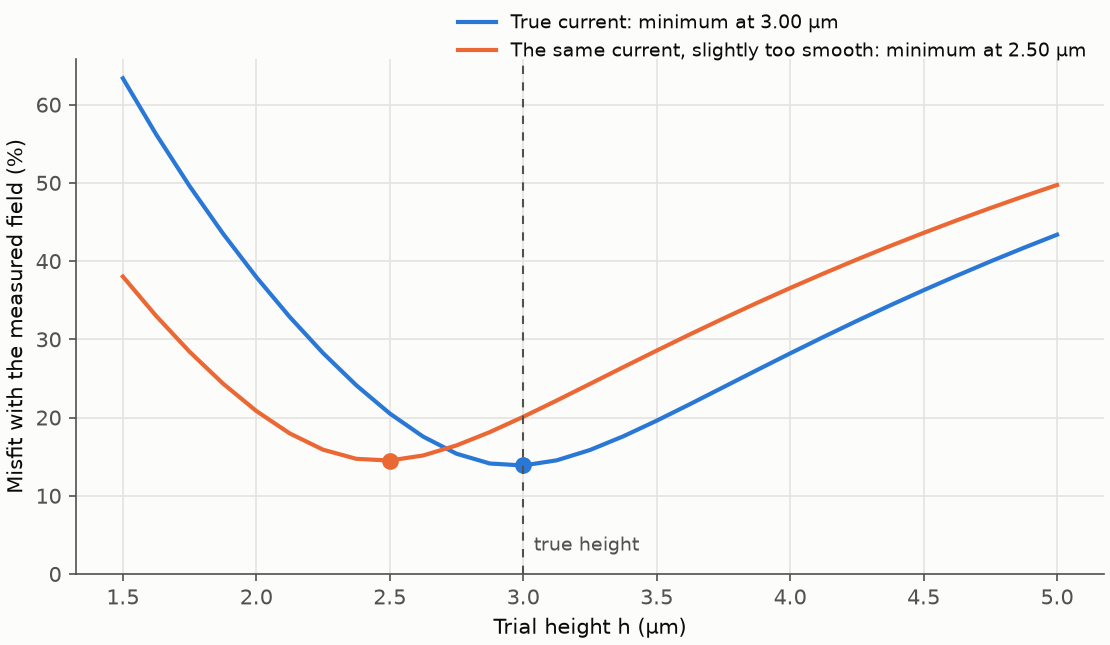
\includegraphics[width=0.8\textwidth]{late_height_misfit}
\caption{The read-out on one simulated layout measured at 3\um. With the true current the misfit has its minimum exactly
at 3\um. With the same current slightly smoothed, the minimum moves to a smaller height.}
\label{fig:late_height}
\end{figure}

\section{The code}

The Fourier transform of the current is the expensive part, and it does not depend on the height. So it is done once:

\begin{code*}{m12_common.py}
    fx, fy = np.fft.rfft2(jx), np.fft.rfft2(jy)
    fz = 1j * (wy * fx - wx * fy) / safe
    return (fx, fy, fz), k, (ny, nx)
\end{code*}

These are the same three lines as the Biot--Savart step of Chapter~\ref{ch:magic}. Then each trial height only needs
one multiplication by $e^{-kh}$ and one inverse transform:

\begin{code*}{m12_common.py}
    decay = 0.5 * mu0_ut * np.exp(-k * height)
    return np.stack([np.fft.irfft2(f * decay, s=shape)[pad:pad + image, pad:pad + image]
                     for f in spectra])
\end{code*}

\begin{code*}{m12_common.py}
    return np.array([relative_l2(field_at(spectra, k, shape, h, image, pad), b).mean()
                     for h in heights])
\end{code*}

The search is done in two passes: a coarse grid in steps of 0.1\um, then a fine grid in steps of 0.01\um\ around the
best coarse value.

\begin{code*}{m12_common.py}
    coarse = misfit_fn(grid)
    h0 = grid[int(np.argmin(coarse))]
    fine_h = np.round(np.arange(h0 - FINE_HALF, h0 + FINE_HALF + 1e-9, FINE_STEP), 3)
\end{code*}

\begin{code*}{m12_common.py}
    edge = bool(h <= lo + 0.1 or h >= h_max - 0.1)
\end{code*}

The last line is a warning flag. If the minimum sits at the end of the grid, the true minimum may lie outside it, and
the result should not be trusted.

A test on the Mac checks the whole thing with a known answer: it builds fields at 1.37, 3.00 and 6.42\um\ from a known
current and recovers each height to 0.01\um. On the server the same computation runs on the GPU:

\begin{code*}{m1_rescore.py}
def read_height(sheet, b, device, h_max=mc.EDGE[1]):
    b32 = torch.as_tensor(np.asarray(b, np.float32), device=device)
    b_norm = (b32 ** 2).sum((-2, -1)).sqrt()
    return mc.read_height(lambda hs: sheet.misfit(hs, b32, b_norm), h_max)
\end{code*}

\section{Why the read-out can be wrong}

Look again at Figure~\ref{fig:late_height}. The orange curve uses a current that is slightly too smooth. Its minimum is
at a \emph{smaller} height. This is the ambiguity of Chapter~\ref{ch:question}, seen from the other side: a smoother
source closer to the sensor gives the same field as a sharper source further away. So:
\begin{itemize}
\item a predicted current that is \textbf{too smooth} reads the height \textbf{too low};
\item a predicted current that is \textbf{too sharp} or too strong reads it \textbf{too high}.
\end{itemize}

\begin{keyidea}[The read-out measures the network, not only the height]
$h^\ast$ is the height at which \emph{this network's current} best explains the data. If the current is right, $h^\ast$ is
the true height. If the current is biased, $h^\ast$ is biased in the matching direction.
\end{keyidea}

\section{On simulation}

50 validation layouts at each standoff, where the truth is known:

\begin{center}
\small
\begin{tabular}{lcccccccc}
\toprule
True standoff (\textmu m) & 1 & 2 & 3 & 4 & 5 & 6 & 8 & 10 \\
\midrule
Run 2, median $h^\ast$ & 1.21 & 2.05 & 3.06 & 4.01 & 4.46 & 4.43 & 3.66 & 2.63 \\
Run 3, median $h^\ast$ & 1.18 & 2.11 & 3.12 & 4.14 & 5.29 & 6.50 & 8.27 & 7.84 \\
\bottomrule
\end{tabular}
\end{center}

\begin{itemize}
\item \textbf{Run 2} reads the height well from 1.5 to 4\um\ (median error 2--5\%). That is its training range. Above it,
the read-out stops following and falls back toward 3--4\um: the network keeps drawing currents that belong to its
training heights.
\item \textbf{Run 3} follows the truth from 1.5 to 8\um: within 15\% for 93\% of images, reading about 5\% high. It fails at
both ends of its range, 1 and 10\um.
\end{itemize}

This is what the one-sided ambiguity predicts: the prior decides the height, so a network knows heights only where it
has learned what sources look like at those heights.

\section{On COMSOL}

At 3\um\ on COMSOL, run 2 reads 2.93--3.01\um\ on all five configurations. Outside 3\um\ it is pulled toward 3: an input
at 2\um\ reads 2.32, and at 4\um\ reads 3.61. Run 3 reads the C1-family coils at 2.97--3.10\um, and \code{IC_4um} at
3.86\um, too high. That fits Chapter~\ref{ch:run3}: on that coil its current is too strong, and a too-strong current
reads high.

One more observation, to be picked up later. On COMSOL \code{L1_C1} at large standoffs, run 3 reads \emph{low}: 6.26 at
7\um, 7.97 at 10\um. On simulation it reads high there. Chapter~\ref{ch:ten_results} finds the reason.

\section{The test that failed}

The review predicted: run 3 fails on the IC coil because each tile picks its own height, so imposing one global height
should rescue it. Under the protocol, that was a decision rule written in advance. The result:

\begin{center}
\begin{tabular}{lc}
\toprule
Run 3 on \code{IC_4um}, 3\um\ to 0.5\um & Error \\
\midrule
Raw & 52.0\% \\
Corrected at its own read-out, 3.86\um & 46.9\% \\
Corrected at the true height, 3\um & 37.3\% \\
Run 2, raw, for comparison & 29.6\% \\
\bottomrule
\end{tabular}
\end{center}

(``Corrected'' is the step of the next chapter.) Even with the true height it stays far from run 2. So the prediction
was wrong, and the review says so.

\begin{keyidea}[The lesson for any future method]
The per-tile decision is baked into the predicted current. A height applied afterwards cannot undo it. A real height
search must \emph{re-run the reconstruction} at each candidate height, and not re-project one prediction. The read-out is
a cheap shortcut, and this experiment showed where the shortcut ends.
\end{keyidea}

\begin{defend}[If your professor asks: does your method estimate the standoff?]
It reads one from the network's own current, with no extra training: within a few per cent inside the range the
network was trained on, on simulation, and 2.93--3.01\um\ at a true 3\um\ on COMSOL. It is not an independent
measurement. It inherits the network's bias, as the IC coil shows, and it has no uncertainty attached yet.
\end{defend}

\chapter{One data-consistency step, and three seeds}\label{ch:consistency}

This is milestone M1b of the review, and it is the step that turned MAGIC-UNet from a tie with FISTA into a win. It is
our addition, not the paper's, so you should be able to derive it on a board.

\section{The problem it solves}

Chapter~\ref{ch:limits} ended with a strange fact: MAGIC-UNet is the best method where the measurement is silent (the
prior band) and the worst of the good methods where the measurement speaks (16.0\% in the measured band, against
FISTA's 9.1\%).

The reason is in how the two work. FISTA's loop compares its guess with the measurement at every iteration. MAGIC-UNet
looks at the measurement once and outputs a current. \textbf{Nothing forces that output to agree with what was measured.}
The check is simple: blur MAGIC-UNet's 0.5\um\ field back up to 3\um\ and compare with the real 3\um\ input. It misses by
17--33\%. The COMSOL truth itself, blurred the same way, misses by 10--17\%.

\section{Deriving the correction}

Call the network's field at 0.5\um\ $X$, the measurement $B$, and the blur between the two heights $H=e^{-k\,\Delta z}$.
We want a new field $X'$ that
\begin{itemize}
\item agrees with the measurement when blurred: $HX'\approx B$;
\item but stays close to the network's answer: $X'\approx X$.
\end{itemize}
Write both wishes as one cost, with a number $\mu$ that says how much the second matters:
\[
\min_{X'}\ |HX'-B|^2+\mu\,|X'-X|^2 .
\]
In Fourier space the blur is just a multiplication, so each frequency can be solved alone. Set the derivative to zero:
\[
H\,(HX'-B)+\mu\,(X'-X)=0
\quad\Longrightarrow\quad
X'=\frac{HB+\mu X}{H^2+\mu}.
\]
Rearranged into ``the old answer plus a correction'':
\[
\boxed{\;X'=X+\frac{H}{H^2+\mu}\,\bigl(B-HX\bigr)\;}
\]
The bracket is the mismatch: the measurement minus the network's field blurred up. The fraction turns that mismatch,
which lives at the measurement height, back into a change at 0.5\um.

\section{What it does at each frequency}

There is a second way to write the same formula that makes it easy to see:
\[
X'=w\cdot\frac{B}{H}+(1-w)\cdot X,\qquad w=\frac{H^2}{H^2+\mu}.
\]
$B/H$ is the plain inverse of the blur: what you get if you trust only the measurement. $X$ is what you get if you trust
only the network. $w$ is a dial between them, and it is different at every frequency:
\begin{itemize}
\item at low frequencies $H\approx1$, so $w\approx1$: \textbf{use the measurement};
\item at high frequencies $H\to0$, so $w\to0$: \textbf{keep the network}.
\end{itemize}
The changeover is where $H^2=\mu$.

\begin{figure}[H]
\centering
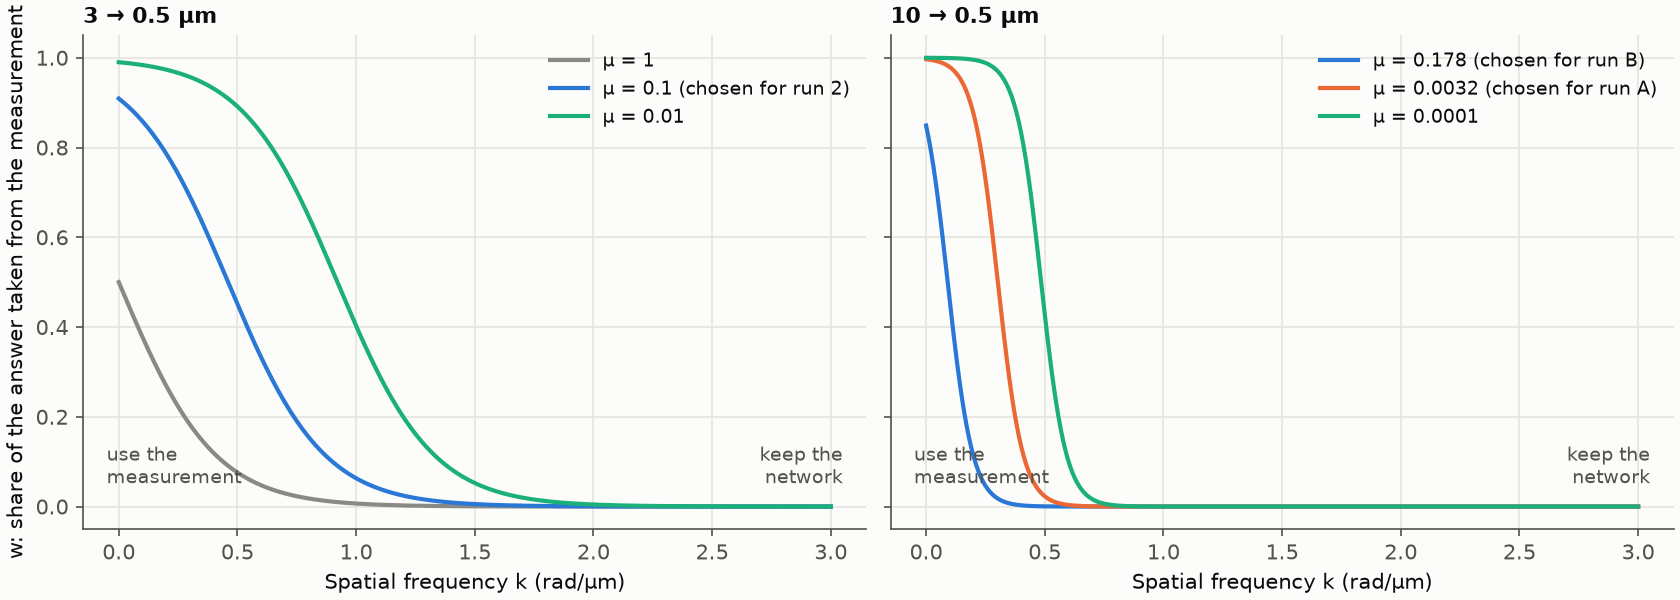
\includegraphics[width=0.95\textwidth]{late_dc_gain}
\caption{The dial $w$: how much of the final answer comes from the measurement, at each frequency. Left: 3\um\ to
0.5\um. Right: 10\um\ to 0.5\um, where the measurement only reaches the lowest frequencies.}
\label{fig:late_dc}
\end{figure}

\begin{keyidea}[Why this is the right kind of fix]
It gives each source of information the frequencies it is good at. The measurement decides the measured band. The
network's prior decides the band above it. That is exactly the split of Chapter~\ref{ch:limits}.
\end{keyidea}

\section{The code}

The whole step is six lines:

\begin{code*}{m12_common.py}
    n = np.asarray(x).shape[-1] + 2 * pad
    _, _, k = wavenumbers(n, dx)
    h = np.exp(-k * dz)
    fx, fb = padded_fft(x, pad), padded_fft(b, pad)
    return crop_ifft(fx + h / (h * h + mu) * (fb - h * fx), pad)
\end{code*}

The last line is the boxed formula. Before the transform the images are padded with 128 pixels of zeros on every
side, and cropped again afterwards. A Fourier transform treats an image as if it repeated forever, and without padding
the left edge would leak into the right.

Two tests check it against known answers: with exact data and $\mu\to0$ it returns the truth, and a prediction that
already agrees with the data is left unchanged.

\section{Choosing $\mu$, without touching COMSOL}

In the review's first diagnostic, three values of $\mu$ were tried directly on COMSOL. That is choosing on the test
data. Under the protocol, $\mu$ is chosen on \emph{simulated} images only, where the true target is known. For each of
17 values from $10^{-4}$ to 1, the corrected field is scored on 50 simulated layouts:

\begin{code*}{m1_rescore.py}
                corr = Corrector(pred.cpu().numpy(), b, z - 0.5, device)
                for m, mu in enumerate(mc.MU_GRID):
                    errors[i, m] = rel(corr(float(mu)), t)
\end{code*}

\begin{code*}{m1_rescore.py}
            mean = errors.mean((0, 2))
            best = int(np.argmin(mean))
            mu_curve[run].append(float(mc.MU_GRID[best]))
\end{code*}

This is repeated at every simulated standoff, which gives a curve $\mu(h)$. \code{Corrector} is the same formula on the
GPU, with the transforms done once so that 17 values are cheap:

\begin{code*}{m1_rescore.py}
    def __call__(self, mu):
        h = self.h
        out = torch.fft.irfft2(self.fx + h / (h * h + mu) * (self.fb - h * self.fx), s=(self.n, self.n))
        return out[..., mc.PAD:-mc.PAD, mc.PAD:-mc.PAD]
\end{code*}

\begin{center}
\small
\begin{tabular}{lcccccccc}
\toprule
Standoff (\textmu m) & 1 & 2 & 3 & 4 & 5 & 6 & 8 & 10 \\
\midrule
Best $\mu$ for run 2 & 0.32 & 0.18 & 0.1 & 0.056 & 0.01 & 0.0018 & 0.00056 & 0.00032 \\
\bottomrule
\end{tabular}
\end{center}

The best $\mu$ falls by about a thousand from 1 to 10\um. Two things drive it. A larger standoff makes $H$ smaller, so a
smaller $\mu$ is needed to keep the same dial setting. And outside its training range run 2 is poor, so the data
deserve more trust.

\section{Using the estimated height}

One thing is still missing. $H$ contains the standoff, and MAGIC-UNet is not supposed to be given the standoff. So the
correction uses the height of Chapter~\ref{ch:height}, read from the network's own current, and looks up $\mu$ on the
curve at that height:

\begin{code*}{m1_rescore.py}
                mu = mc.mu_at(row['h_star'], args.standoffs, mu_curve[run])
                fixed = Corrector(pred.cpu().numpy(), b, row['h_star'] - 0.5, device)(mu)
\end{code*}

\begin{code*}{m12_common.py}
def mu_at(h, standoffs, mus):
    """log10 mu linearly interpolated in h; held constant outside the simulated range (protocol M1b)."""
    return float(10 ** np.interp(h, np.asarray(standoffs, float), np.log10(np.asarray(mus, float))))
\end{code*}

So the full pipeline is: network $\to$ current $\to$ field at 0.5\um\ $\to$ read $h^\ast$ $\to$ one correction at $h^\ast$.
Nothing in it uses the true standoff.

\section{The result}

\begin{center}
\small
\begin{tabular}{lcccc}
\toprule
COMSOL, 3\um\ to 0.5\um, 15 pairs & Raw & Measured band & Prior band & Low-passed \\
\midrule
MAGIC-UNet run 2 & 27.0\% & 16.0\% & 14.6\% & 22.0\% \\
\quad + correction at the true height & 24.3\% & 10.9\% & 14.6\% & 18.5\% \\
\quad + correction at $h^\ast$ (standoff not given) & \textbf{24.3\%} & 11.0\% & 14.6\% & 18.5\% \\
FISTA, 1{,}000 iterations & 26.7\% & 9.1\% & 19.3\% & 21.9\% \\
FISTA, 925 iterations (the baseline from Ch.~\ref{ch:fista_depth}) & 26.9\% & & & \\
\bottomrule
\end{tabular}
\end{center}

\begin{keyidea}[It did exactly what the derivation promised]
The measured-band error fell from 16.0\% to 11.0\%. The prior-band error did not move: 14.6\% before and after. Not
knowing the height cost nothing here (24.3\% both ways), because the read-out at 3\um\ is good.
\end{keyidea}

On simulation the correction lowers the error at every standoff for both runs (at 3\um: 15.1\% to 13.7\% for run 2), and
on COMSOL it helps on all 40 rows that were scored.

\begin{careful}[An honest correction]
The review's first diagnostic gave 24.2\% on the two local configurations, with $\mu$ picked from three values on that
test data. Like for like, with $\mu$ from simulation, the same two configurations give 25.1\%. So choosing on the test
data had made the number 0.9 points too good. Small, but it is exactly the effect the protocol exists to prevent.
\end{careful}

\section{Three seeds}

A trained network depends on random numbers: the starting weights, the order of the batches, the noise drawn in
training. The \emph{seed} fixes them. Change the seed and you get a slightly different network. So far every network had
one seed, and a difference between two methods could simply be luck.

Two more copies of run 2 were trained, identical except for the seed. And \emph{before} they finished, the rule for
reading them was written down (amendment A4):

\begin{keyidea}[The rule]
``MAGIC-UNet beats FISTA on a set of pairs'' may be written only if \textbf{all three seeds} score below FISTA on that
set. If even one does not, the result is written as ``not distinguishable on this test set'', whatever the average
says. FISTA has no seed: it gives the same answer every time.
\end{keyidea}

\begin{center}
\small
\setlength{\tabcolsep}{4pt}
\begin{tabular}{llcccccl}
\toprule
 & Set & Seed 0 & Seed 1 & Seed 2 & FISTA-1000 & FISTA-925 & Verdict \\
\midrule
Raw & 15 pairs & 27.0\% & 27.2\% & 26.7\% & 26.7\% & 26.9\% & not distinguishable \\
Raw & \code{IC_4um} & 29.6\% & 29.8\% & 32.6\% & 27.2\% & 27.2\% & not distinguishable \\
\midrule
Corrected & 15 pairs & 24.3\% & 24.5\% & 24.5\% & 26.7\% & 26.9\% & \textbf{beats FISTA} \\
Corrected & C1 family & 23.8\% & 23.7\% & 22.9\% & 26.6\% & 26.8\% & \textbf{beats FISTA} \\
Corrected & \code{IC_4um} & 26.4\% & 27.5\% & 30.9\% & 27.2\% & 27.2\% & not distinguishable \\
\bottomrule
\end{tabular}
\end{center}

The rule was first applied against FISTA-1000. Against FISTA-925, the baseline of Chapter~\ref{ch:fista_depth}, every
verdict is the same. Read the last row carefully. Seed 0, the original run 2, is 0.8 points better than FISTA on \code{IC_4um}. Seed 2 is 3.6
points worse. The earlier ``win'' on that coil was luck. \code{IC_4um} is one shape with three component images, and its
seeds spread over 4.4 points, more than any margin on it.

\begin{keyidea}[The fair summary at 3\um, and the one to use in your report]
With one data-consistency step, MAGIC-UNet beats a converged FISTA on the 15 pairs and on the C1-family coils, for
every seed, without being told the standoff: 24.3--24.5\% against 26.9\% for FISTA at its best depth (26.7\% at
1{,}000 iterations). On \code{IC_4um} the two are \textbf{not
distinguishable}. The paper's network on its own ties FISTA.
\end{keyidea}

\begin{defend}[If your professor asks: is the data-consistency step from the paper?]
No. It is our addition and must be labelled so every time. It is one linear step with one number $\mu$, chosen on
simulated data, at a height the network estimates itself. It changes only the frequencies the measurement carries.
\end{defend}

\begin{defend}[If your professor asks: why not put FISTA's data consistency inside the network?]
That is the method the review recommends for the future: a learned current prior inside several data-consistency
steps, with a search over height. One step applied afterwards was the cheapest possible test of whether that direction
is right. It was.
\end{defend}

\begin{defend}[If your professor asks: why only three seeds?]
Each run takes 4 to 8 hours on the one GPU. Three is the minimum that lets a rule like ``all seeds below the
baseline'' mean something, and the rule was written before the seeds finished.
\end{defend}

\chapter{What COMSOL really computes}\label{ch:comsol}

This chapter covers 13 and 14 November. It answers a question that had been open since 1 November, and its answer
decided how the 10\um\ work was done.

\section{The puzzle}

Our simulator draws wires and computes their field with exact physics. Close to the coil it agreed with COMSOL to
within the mesh noise. Higher up it drifted away, and at 10\um\ it was off by 65\%, 61\% and 134\% for $B_x$, $B_y$ and
$B_z$. Either our physics was wrong, or COMSOL's was. On 13 November Hari sent the COMSOL model files: the full
reports, the coil drawing, and exports on a second, finer mesh. Everything below was computed from them by the
scripts in \code{scripts/comsol_check/}. Nothing was trained.

\section{The model}

\begin{center}
\small
\begin{tabularx}{\textwidth}{>{\raggedright\arraybackslash}p{3.2cm}X}
\toprule
Item & In the COMSOL model \\
\midrule
Physics & Magnetic Fields, a \emph{stationary} study: nothing changes in time \\
Domain & One block of air, $140\times140\times90$\um \\
Walls & ``Magnetic insulation'' on all six faces: no field line may cross a wall \\
Coil & Wires 2.00\um\ wide, carrying 600\,\textmu A, as a sheet of zero thickness at $z=0$ \\
Leads & They run to the wall; the current returns through the wall \\
One solve for four data sets & \code{L1_C1} and the three multi-coil sets come from the same model and mesh \\
Mesh & 284{,}696 tetrahedra (``Extra Fine''), and a second export on 1{,}372{,}173 (``Extremely Fine'') \\
Export & A cut plane at each height, $1400\times1400$ points at 0.1\um \\
\bottomrule
\end{tabularx}
\end{center}

Two facts in this table already explain old observations. The four C1 configurations share one solve, so they share
their mesh noise (Chapter~\ref{ch:review}). And the exported window is the \emph{whole} box, wall to wall.

\section{First check: the quarter turn}

Since October the code had rotated COMSOL's components by a quarter turn, because it made the data look right. Now the
reason is known. The columns \code{cpl1x} and \code{cpl1y} of the export are the cut plane's own axes, and COMSOL turned
them against the model's axes. The field columns are in the model's axes. So along the image axes, the components are

\begin{code*}{comsol_check/decay_rate.py}
def frame(B):
    Bx, By, Bz = B.astype(float); return -By, Bx, Bz
\end{code*}

How do we know this is right and not just convenient? With the test of Chapter~\ref{ch:limits}: the three components of
a real field are tied together. With this mapping the tie holds to 6\%. With the naive labels it fails completely
(100\%).

\section{Second check: the walls are there, but they are not the cause}

A closed box with insulating walls leaves fingerprints. The field component pointing into each wall should vanish,
and it does: 0.2--0.6\% of the typical field at the window edges. The average of $B_z$ over a plane should be zero, and
it is, to four decimals at every height.

Our simulator has no walls. It pads with zeros, as if space went on forever. Is that the problem? No. Propagating
COMSOL's own 0.5\um\ field up to 10\um\ with an exact model of the box (mirror images in every wall) misses COMSOL's
10\um\ field by 50.1\%. Without walls it misses by 50.8\%. The walls change almost nothing.

\section{Measuring how fast the field really decays}\label{sec:cm_decay}

So measure the decay directly. Physics says: between two heights $\Delta z$ apart, a ripple of frequency $k$ shrinks by
$e^{-k\,\Delta z}$. Take two COMSOL planes, look at one band of frequencies in both, and ask by what factor it shrank.
The decay rate is minus the logarithm of that factor, divided by $\Delta z$. If COMSOL obeys physics, the rate equals
$k$.

\begin{code*}{comsol_check/decay_rate.py}
    for lo, hi in bands:
        m = (K >= lo) & (K < hi)
        num = sum(np.vdot(a[m], b[m]) for a, b in zip(F1, F2))
        den = sum(np.vdot(a[m], a[m]) for a in F1)
        r = (num/den).real
        kc = np.sqrt(np.mean(K[m]**2))
        out.append((kc, -np.log(max(r, 1e-12))/dz))
\end{code*}

\code{F1} and \code{F2} are the spectra of the lower and the upper plane. \code{num/den} is the least-squares factor
between them in that band, over all three components. The last line turns it into a rate.

\begin{center}
\small
\begin{tabular}{lccccccc}
\toprule
Band $k$ (rad/\um) & 0.027 & 0.075 & 0.109 & 0.155 & 0.216 & 0.303 & 0.432 \\
\midrule
Physics predicts: rate $=k$ & 0.027 & 0.075 & 0.109 & 0.155 & 0.216 & 0.303 & 0.432 \\
Measured, 0.5 to 3\um & 0.103 & 0.128 & 0.144 & 0.189 & 0.240 & 0.329 & 0.445 \\
Measured, 3 to 6\um & 0.104 & 0.126 & 0.141 & 0.187 & 0.238 & 0.327 & 0.435 \\
Measured, 6 to 10\um & 0.106 & 0.127 & 0.141 & 0.188 & 0.237 & 0.329 & 0.420 \\
\midrule
$\sqrt{k^2+0.10^2}$ & 0.104 & 0.125 & 0.148 & 0.184 & 0.238 & 0.319 & 0.443 \\
\bottomrule
\end{tabular}
\end{center}

\begin{keyidea}[What the table says]
At the lowest frequency COMSOL's field decays almost \emph{four times} faster than physics allows (0.103 against
0.027). The excess is the same at every height, and one formula fits every band:
\[
\text{rate}=\sqrt{k^2+k_0^2},\qquad k_0\approx0.10\ \text{rad/\um}.
\]
For fine detail ($k\gg k_0$) the extra term does not matter. For broad structure it dominates.
\end{keyidea}

That is why the problem only shows at large standoffs. At 0.5\um\ only 11\% of the field lies below $k=0.1$\,rad/\um. At
10\um, where everything fine has already died away, 70\% of it does.

\section{One constant closes the gap}

If this is the whole story, then putting $k_0$ into our own model should make it match COMSOL. Starting from the exact
coil drawing:

\begin{center}
\footnotesize
\setlength{\tabcolsep}{4pt}
\begin{tabular}{lccc}
\toprule
Ours against COMSOL, $B_x$ / $B_y$ / $B_z$ & Free space & Box walls & Walls and $k_0=0.10$ \\
\midrule
at 3\um & 14.0 / 12.0 / 24.7\% & 14.0 / 13.0 / 25.1\% & 11.0 / 10.5 / 10.9\% \\
at 5\um & 23.2 / 19.9 / 45.9\% & 23.1 / 21.4 / 45.7\% & 11.3 / 11.6 / 12.3\% \\
at 10\um & 64.9 / 60.5 / 134.2\% & 64.5 / 57.7 / 128.9\% & \textbf{10.1 / 11.8 / 12.4\%} \\
\bottomrule
\end{tabular}
\end{center}

With $k_0$ the mismatch is 10--12\% at every height, and that is about the size of COMSOL's own mesh noise. The amplitude
comes out right too (scale 1.00). On a configuration that was not used to find $k_0$ (all four coils, at 12.5\um) the
mismatch falls from 83 / 75 / 66\% to 10 / 11 / 10\%.

\begin{figure}[H]
\centering
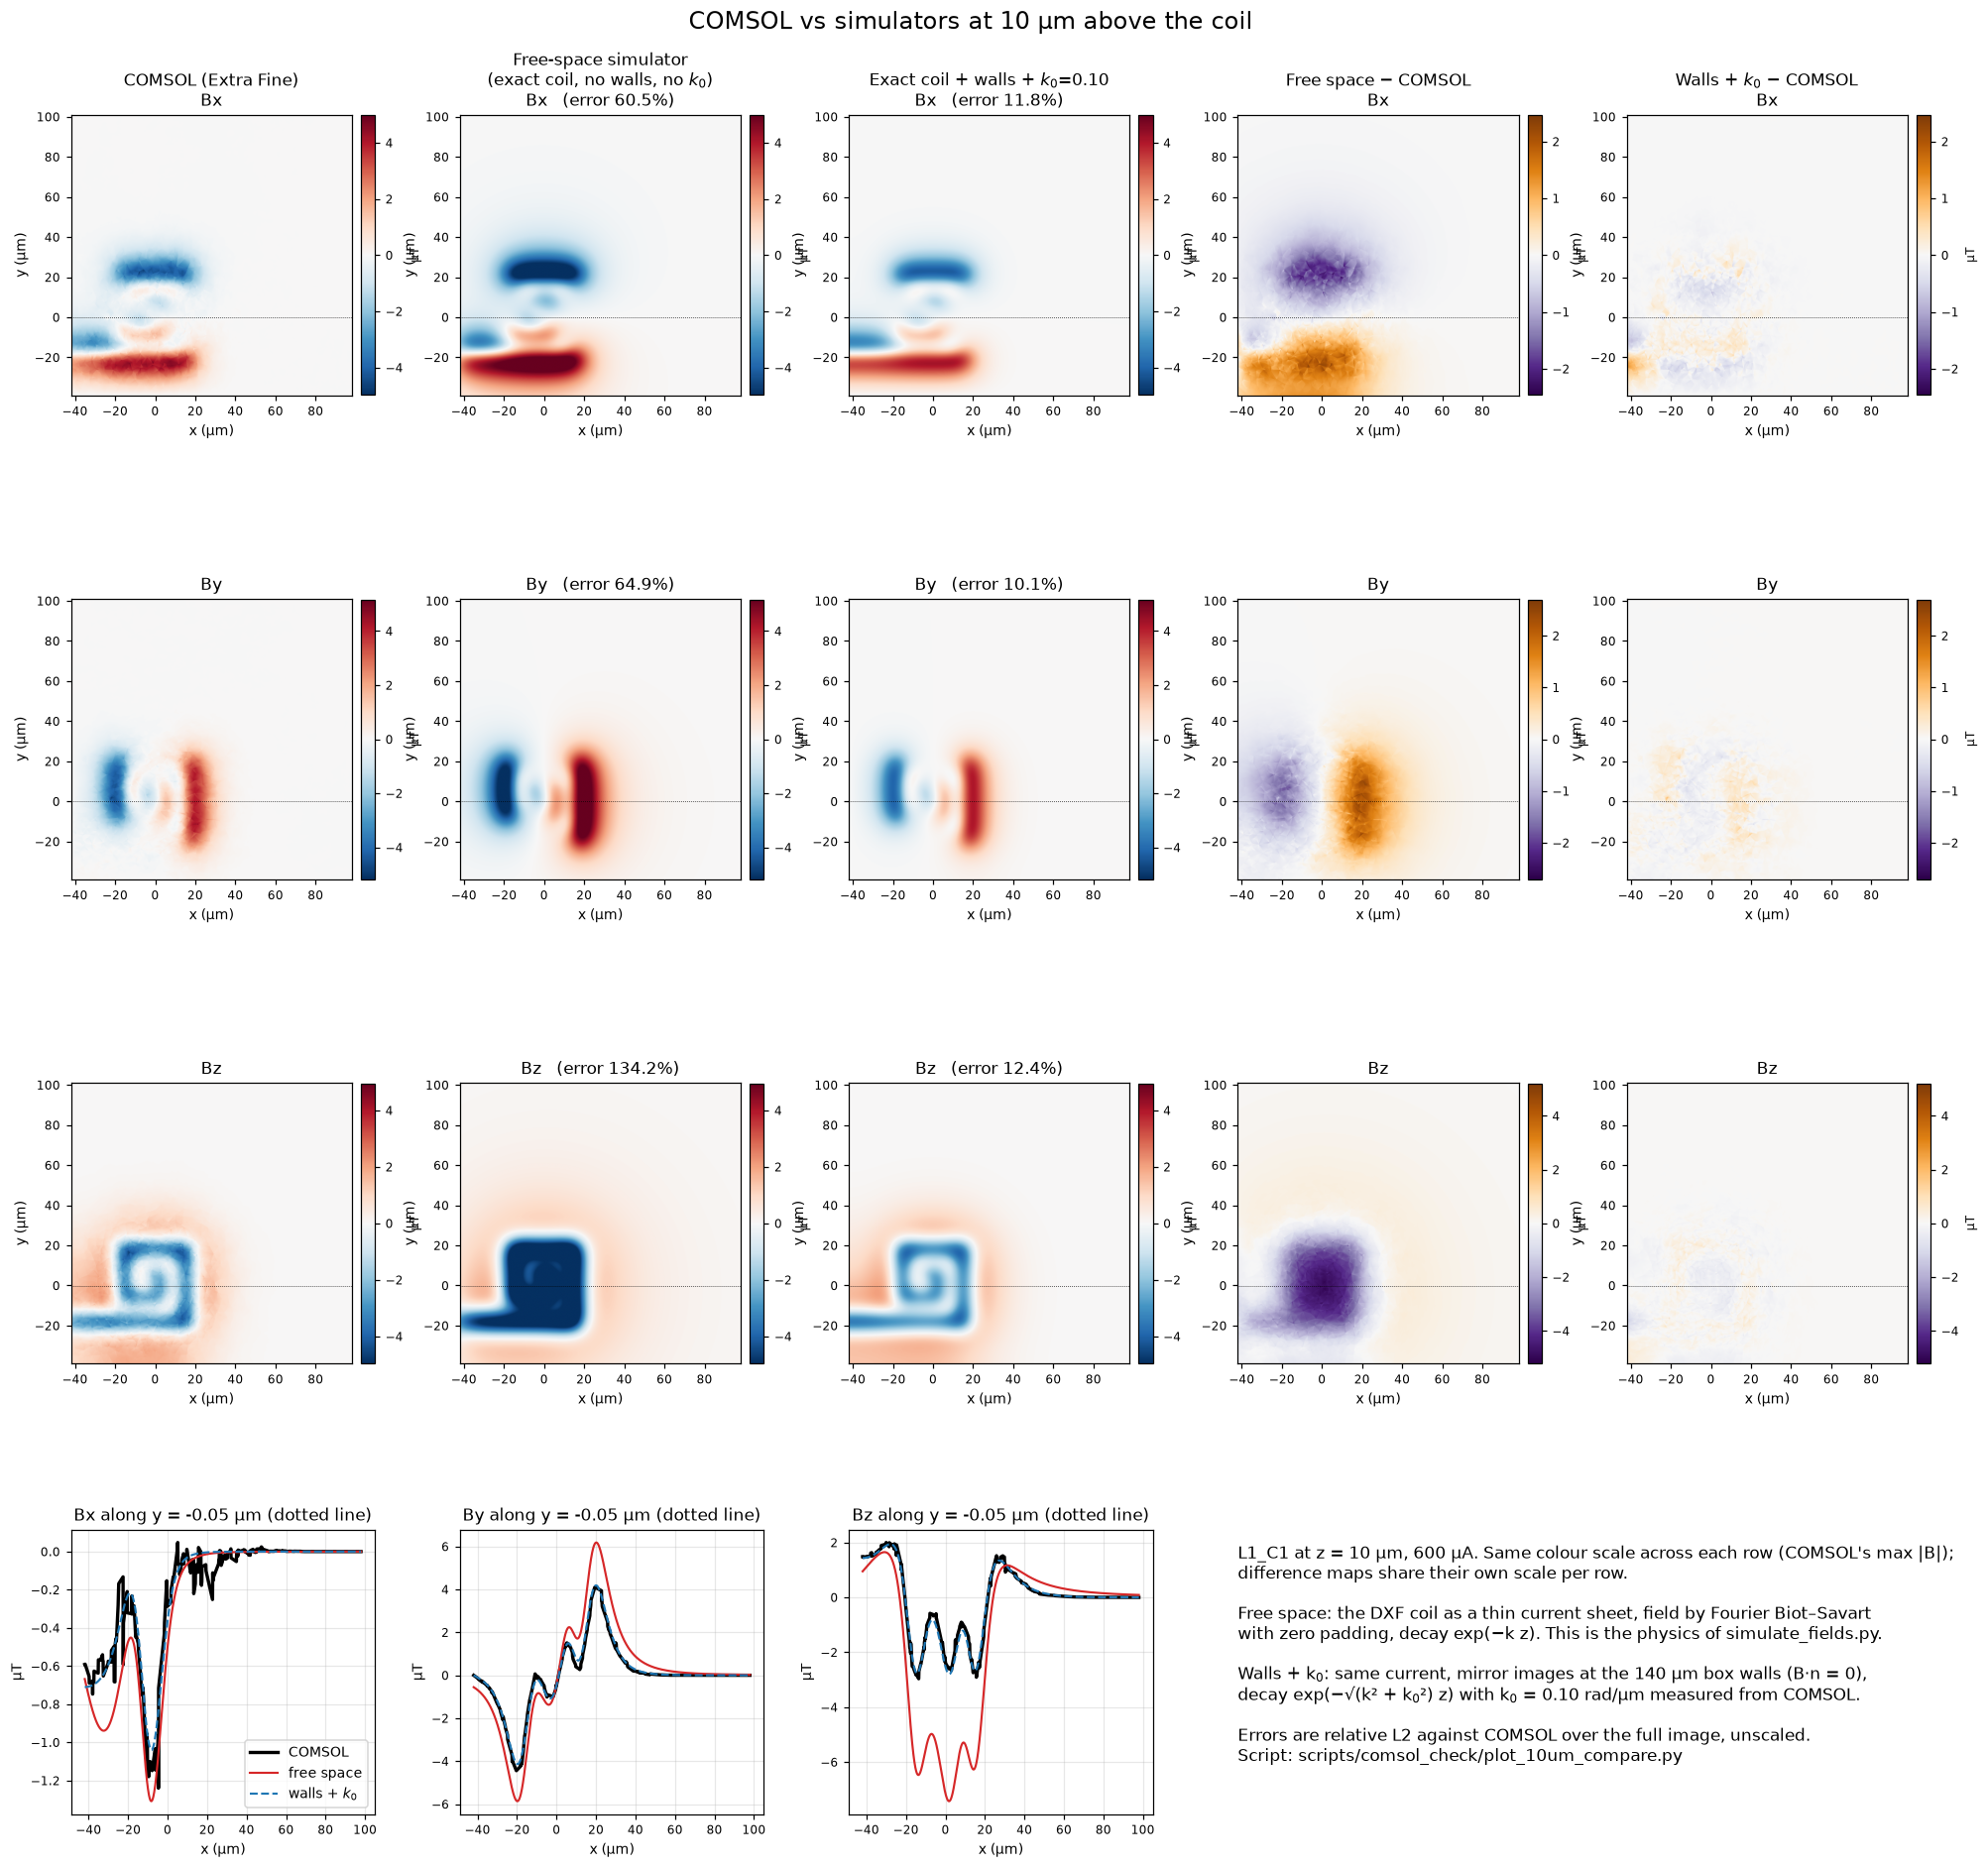
\includegraphics[width=\textwidth]{cm_compare_10um}
\caption{\code{L1_C1} at 10\um. First column: COMSOL. Second: our free-space physics with the exact coil. Third: the same
with walls and $k_0$. Last two columns: the differences. Bottom: cuts through the middle.}
\label{fig:cm_compare}
\end{figure}

\section{Why $k_0$ cannot be physics}

Here is the argument, in two steps you can say out loud.

\textbf{Step 1.} In air there is no current. A static magnetic field in a region with no current must satisfy Laplace's
equation, $\nabla^2B=0$. That forces the decay $e^{-kz}$ and nothing else. COMSOL's field instead satisfies
$\nabla^2B\approx k_0^2\,B$.

\textbf{Step 2.} Amp\`ere's law says the curl of $B$ is the current: $\nabla\times B=\mu_0J$. In empty air $J=0$, so the
curl must be zero. We can test this on COMSOL's own numbers, with no model of ours involved. The horizontal parts of
the curl are
\[
(\nabla\times B)_u=\frac{\partial B_z}{\partial v}-\frac{\partial B_v}{\partial z},\qquad
(\nabla\times B)_v=\frac{\partial B_u}{\partial z}-\frac{\partial B_z}{\partial u}.
\]
The slopes along the plane come from one plane. The slopes in $z$ come from two planes 1\um\ apart:

\begin{code*}{comsol_check/ampere_test.py}
    dzB = [np.real(np.fft.ifft2(b - a))[:N, :N]/dz for a, b in zip(F1, F2)]
    dvBz = np.real(np.fft.ifft2(1j*KV*Fm[2]))[:N, :N]
    duBz = np.real(np.fft.ifft2(1j*KU*Fm[2]))[:N, :N]
    cu = dvBz - dzB[1]
    cv = dzB[0] - duBz
\end{code*}

In each of the last two lines, two terms should cancel exactly. The table gives what is left, as a fraction of the
size of the terms:

\begin{center}
\begin{tabular}{lccc}
\toprule
Between planes & COMSOL & Exact physics (control) & Our model with $k_0=0.10$ \\
\midrule
2 and 3\um & 0.27 & 0.011 & 0.25 \\
3 and 4\um & 0.33 & 0.010 & 0.30 \\
6 and 7\um & 0.41 & 0.007 & 0.44 \\
9 and 10\um & 0.52 & 0.004 & 0.57 \\
\bottomrule
\end{tabular}
\end{center}

The control column runs the \emph{same} estimate on a field from exact physics and gets about 1\%, so the estimate
itself is sound. COMSOL's curl is 27--52\% of the terms that should cancel. In other words, COMSOL's solution has
current flowing in empty air. It runs opposite to the coil current beneath it, like a screening current.

\begin{figure}[H]
\centering
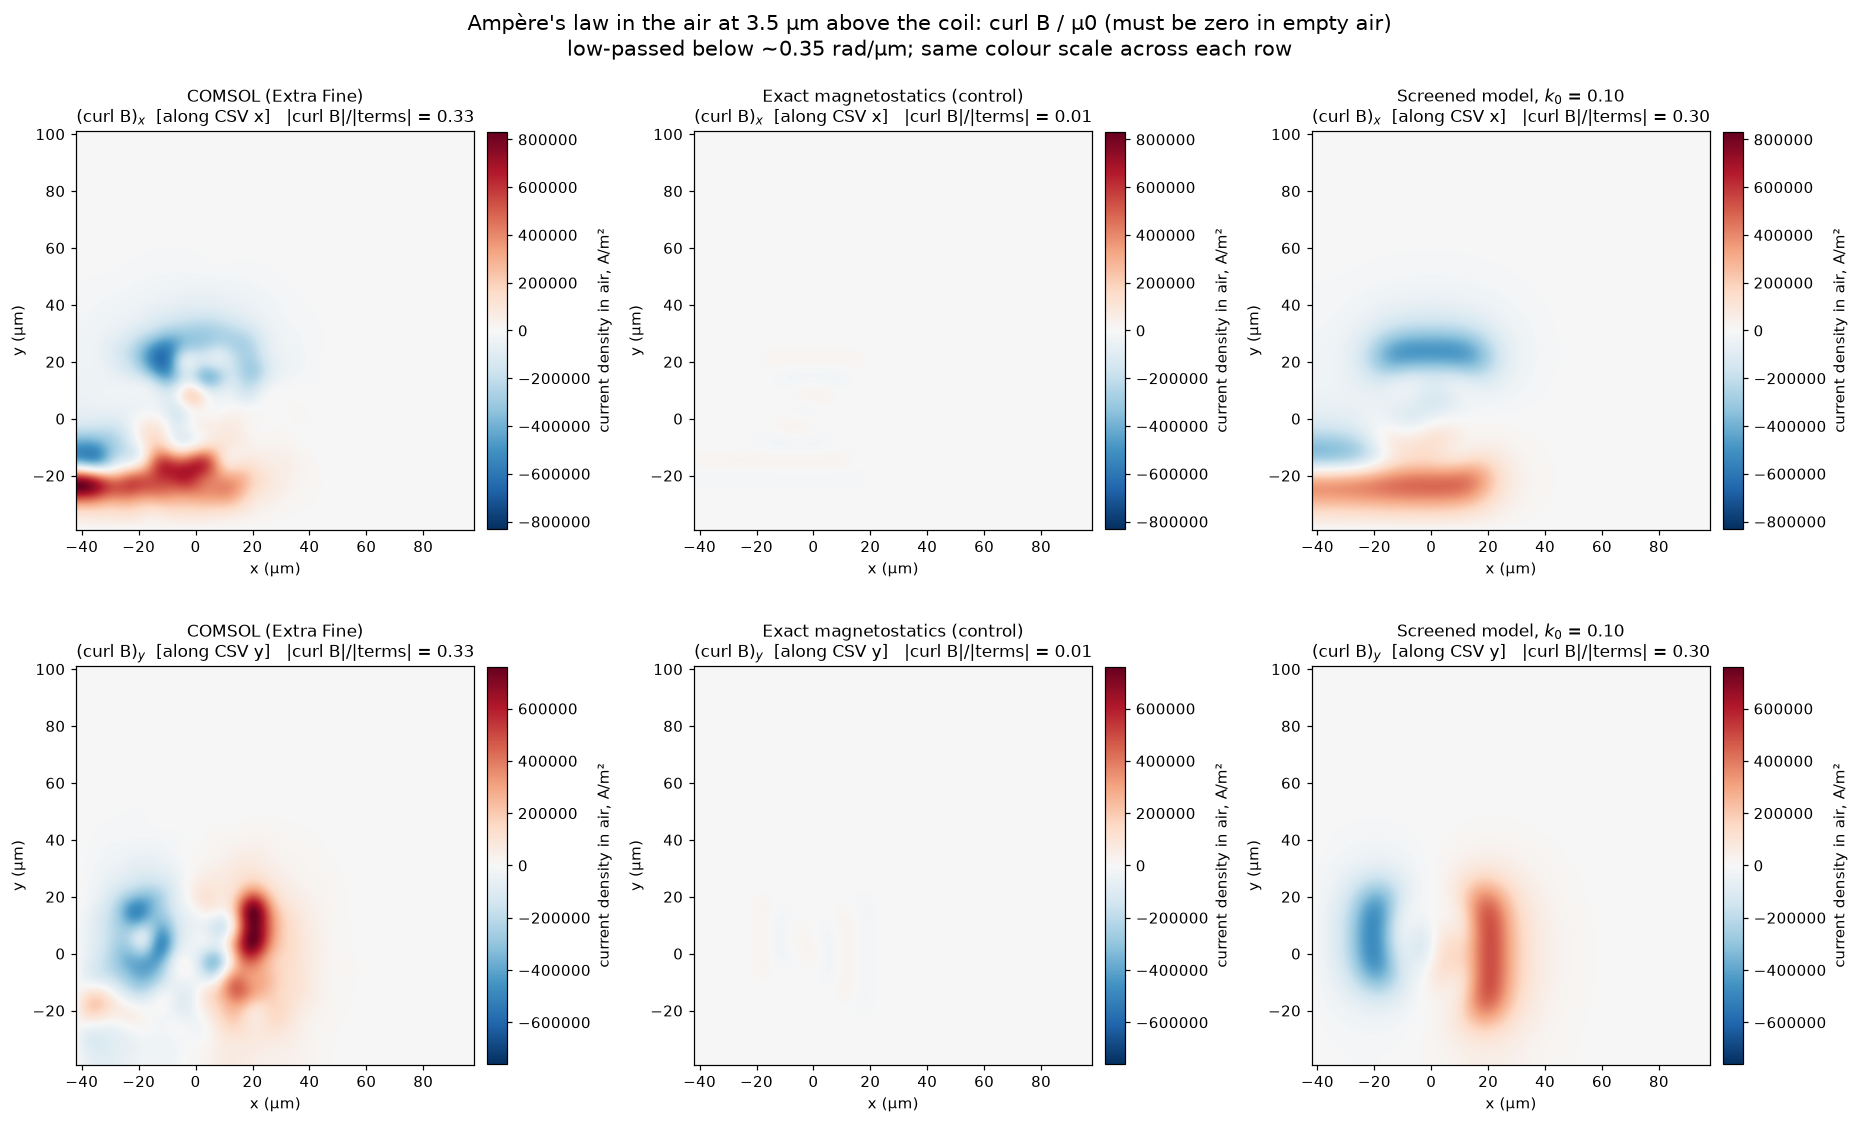
\includegraphics[width=\textwidth]{cm_ampere_air_current}
\caption{The curl of $B$ in the air at 3.5\um, which must be zero. Left: COMSOL. Middle: exact physics. Right: our model
with $k_0$, which reproduces COMSOL's pattern.}
\label{fig:cm_ampere}
\end{figure}

\begin{keyidea}[$k_0$ is not physics]
The air in the model has no conductivity and the study is stationary, so no real current can flow there. And $k_0$ gets
\emph{larger} on the finer mesh (0.12--0.17). A physical effect would not depend on the mesh, and a discretisation
error would shrink on a finer one. So this is a property of how the model was solved.
\end{keyidea}

\begin{careful}[What is not known]
The cause is not established. The candidates are: the iterative solver stopped with an error that is smooth in space;
a regularisation term in the formulation that acts like a weakly screening medium; or a setting in the model file that
the report does not show. One re-solve with a direct solver would separate them. It has been suggested to Hari and has
not been done. The IC coil comes from a different model, for which we have no report; its exports show the same
signature with $k_0\approx0.07$--0.095.
\end{careful}

\section{Is our own simulator right?}

Finding a fault in COMSOL does not prove that we are right. So the simulator was checked against a method that shares
nothing with it: adding up the Biot--Savart law directly along 81 thin filaments of a square loop.

\begin{center}
\begin{tabular}{lccccc}
\toprule
Height & 0.5\um & 1\um & 3\um & 10\um & 20\um \\
\midrule
Simulator against direct Biot--Savart ($B_z$) & 0.54\% & 0.44\% & 0.36\% & 0.74\% & 1.98\% \\
\bottomrule
\end{tabular}
\end{center}

Under 1\% up to 10\um. The rise at 20\um\ has a known cause: the Fourier transform treats the canvas as repeating, and
the loop's far field wraps around. The lesson for high standoffs is to keep the padding generous.

\section{Mesh noise, measured directly}

The same coil on two meshes is two noisy pictures of one true field. Their difference shows the noise:

\begin{center}
\begin{tabular}{lcccc}
\toprule
Frequency band at 0.5\um\ (rad/\um) & below 1 & 1 to 2 & 2 to 2.9 & above 2.9 \\
\midrule
Difference between the meshes, relative & 0.02--0.05 & 0.1--0.2 & about 1.0 & about 1.4 \\
\bottomrule
\end{tabular}
\end{center}

Two independent noise images differ by $\sqrt2\approx1.41$ times one of them. So above 2.9\,rad/\um\ both exports are
pure noise. This is the second confirmation of the noise edge promised in Chapter~\ref{ch:limits}, by a route that
uses no Maxwell equations.

\section{The switch in our simulator}

The simulator can imitate COMSOL's decay if asked. It is one extra term in the exponent:

\begin{code*}{simulate_fields.py}
        decay = 0.5 * MU0_UT * np.exp(-k * z_ref
                                      - np.sqrt(k ** 2 + k0 ** 2) * (z - z_ref))
\end{code*}

Up to the reference plane \code{z_ref} (0.5\um) the decay is the physical $e^{-kz}$. Above it, the rate is
$\sqrt{k^2+k_0^2}$. The default says what we think of it:

\begin{code*}{simulate_fields.py}
    decay_k0=0.0,           # rad/um; nonzero only mimics COMSOL, not physics
\end{code*}

Chapter~\ref{ch:ten_results} uses this switch for one experiment.

\section{The decision}

\begin{center}
\small
\begin{tabularx}{\textwidth}{>{\raggedright\arraybackslash}p{4.6cm}X}
\toprule
Option & What it means \\
\midrule
Add $k_0$ to the simulator and the solvers & COMSOL scores at 5--12\um\ become meaningful, but every model learns a
numerical artefact that a real QDM does not have \\
\textbf{Keep free space} (chosen, 14 November) & Train and test on physically correct data, and report COMSOL above about
4\um\ as a second check with this chapter as the warning \\
Ask for a corrected re-solve & The clean fix; done for L1\_C1 on 14--16 November, and it removed $k_0$ (next section) \\
\bottomrule
\end{tabularx}
\end{center}

\section{Confirmed: the solver tolerance (17 November)}

We asked for one re-solve with a tighter solver. The direct solver could not be used: on this model it stops with
``relative error $1.1\times10^{4}$, returned solution is not converged'', which is what a singular system does (the
vector-potential formulation has no gauge fixing). So Ritaban re-ran the iterative solver with its relative tolerance
tightened to $10^{-8}$, same model, same mesh, and exported L1\_C1 at 0.5, 3 and 10\um.

\begin{figure}[h]
\centering
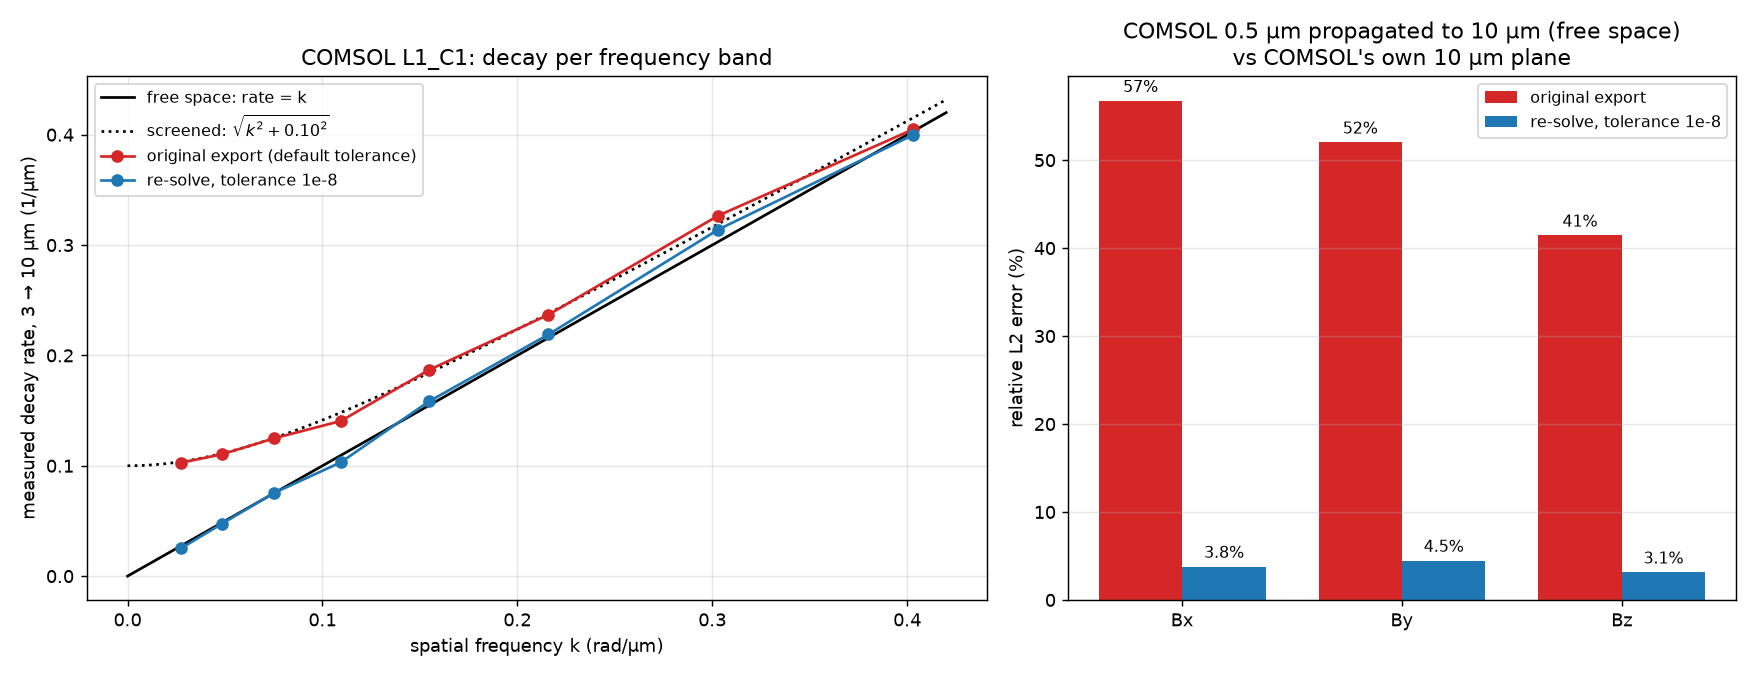
\includegraphics[width=\textwidth]{cm_tolerance_resolve}
\caption{Left: decay rate per frequency band between 3 and 10\um. The original export (red) follows the screened law
$\sqrt{k^2+0.10^2}$; the re-solve (blue) follows free space, rate $=k$. Right: COMSOL's own 0.5\um\ field
propagated to 10\um\ in free space, against COMSOL's 10\um\ plane.}
\end{figure}

\begin{center}
\small
\begin{tabular}{lcc}
\toprule
Check (Bx / By / Bz) & Original export & Re-solve, tolerance $10^{-8}$ \\
\midrule
0.5\um\ propagated to 10\um, against COMSOL 10\um & 57 / 52 / 41\% & \textbf{3.8 / 4.5 / 3.1\%} \\
Our exact-coil simulator (free space) at 10\um & 65 / 58 / 129\% & \textbf{3.2 / 3.2 / 9.3\%} \\
Our exact-coil simulator (free space) at 3\um & 14 / 13 / 25\% & 9.5 / 8.7 / 8.5\% \\
Extra decay $k_0$ & $\approx 0.10$ rad/\um & none \\
\bottomrule
\end{tabular}
\end{center}

\begin{keyidea}[What the re-solve settles]
The extra decay was the default solver tolerance. With a tight tolerance COMSOL obeys free-space magnetostatics, and our
simulator matches it to a few per cent at 10\um. The original exports were off by 39--58\% of the correct field at 10\um\ (60--120\% if the
difference is divided by the original export instead, which is weaker), 9--20\% at 3\um\ and 3--8\% at 0.5\um. Only L1\_C1 at three heights has been re-solved so far; every other COMSOL file still
needs a re-export before it can serve as a clean test.
\end{keyidea}

\section{And Amp\`ere's law? Answered on a single plane}

The re-solve has only three planes (0.5, 3, 10\um), so the test with planes 1\um\ apart cannot be repeated. It does
not need to be. Because $\mathbf{B} = \nabla\times\mathbf{A}$, $\nabla\cdot\mathbf{B}=0$ always, and each Fourier
mode $\mathbf{B}\propto e^{i\mathbf{k}\cdot\mathbf{r}-\gamma z}$ obeys
\begin{equation}
B_z = \frac{i\,\mathbf{k}\cdot\mathbf{B}_t}{\gamma}.
\end{equation}
Amp\`ere's law, $\nabla\times\mathbf{B}=0$, holds if and only if $\gamma = k$. So on one plane the ratio
$R(k) = B_z/[\,i\,\mathbf{k}\cdot\mathbf{B}_t/k\,]$ must be 1 in every band. A screened field gives
$k/\sqrt{k^2+k_0^2}$.

\begin{figure}[h]
\centering
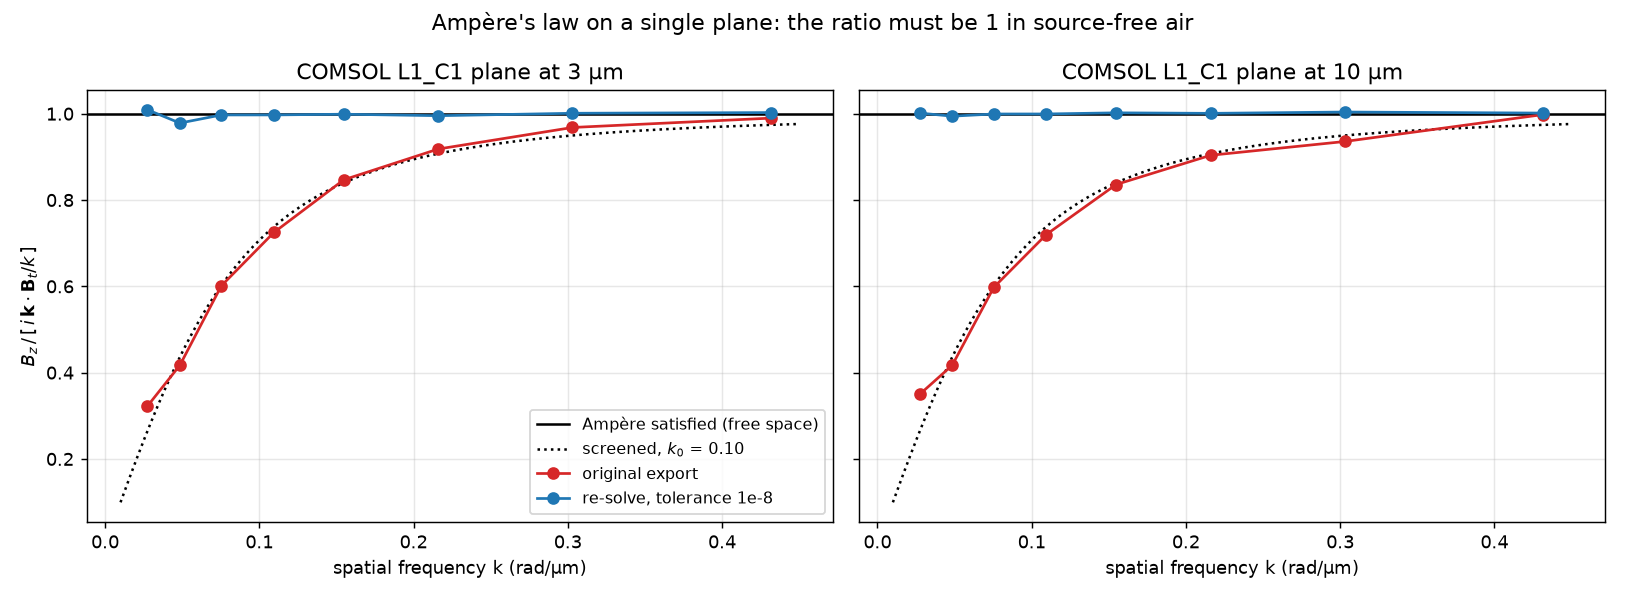
\includegraphics[width=\textwidth]{cm_ampere_single_plane}
\caption{The single-plane Amp\`ere test. The original export (red) follows the screened law with $k_0=0.10$; the
re-solve (blue) gives 1.00 in every band at 3 and at 10\um.}
\end{figure}

\begin{keyidea}[The answer]
The original export had current flowing in empty air because of a loose solver tolerance. With the tolerance at
$10^{-8}$ the field satisfies Amp\`ere's law to 1--2\% in the lowest bands and better than 0.5\% above. The air current
was numerical, and it is gone.
\end{keyidea}

\section{Seeing it: three versions of the same coil}

Numbers like ``58\% off'' are easy to read past. So here is the same coil, \code{L1_C1}, three ways:
\begin{itemize}
\item \textbf{Original export}: what we used for every COMSOL score until 17 November, solved with COMSOL's default
tolerance.
\item \textbf{Re-solve}: the same model and mesh, solved with the tolerance tightened to $10^{-8}$.
\item \textbf{Our simulator}: the physics of our training data (Chapter~\ref{ch:simulation}): a thin current sheet at
$z=0$, the thin-sheet Biot--Savart formulas, and decay $e^{-kz}$. The current is the exact coil from the drawing
(\code{Gemetry_C1.dxf}), 600\,\textmu A, spread over each 2\um\ wire by a conduction solve. Nothing is fitted: no scale, no
height, no offset. Only the direction of the current is read from the data.
\end{itemize}

\begin{sidewaysfigure}
\centering
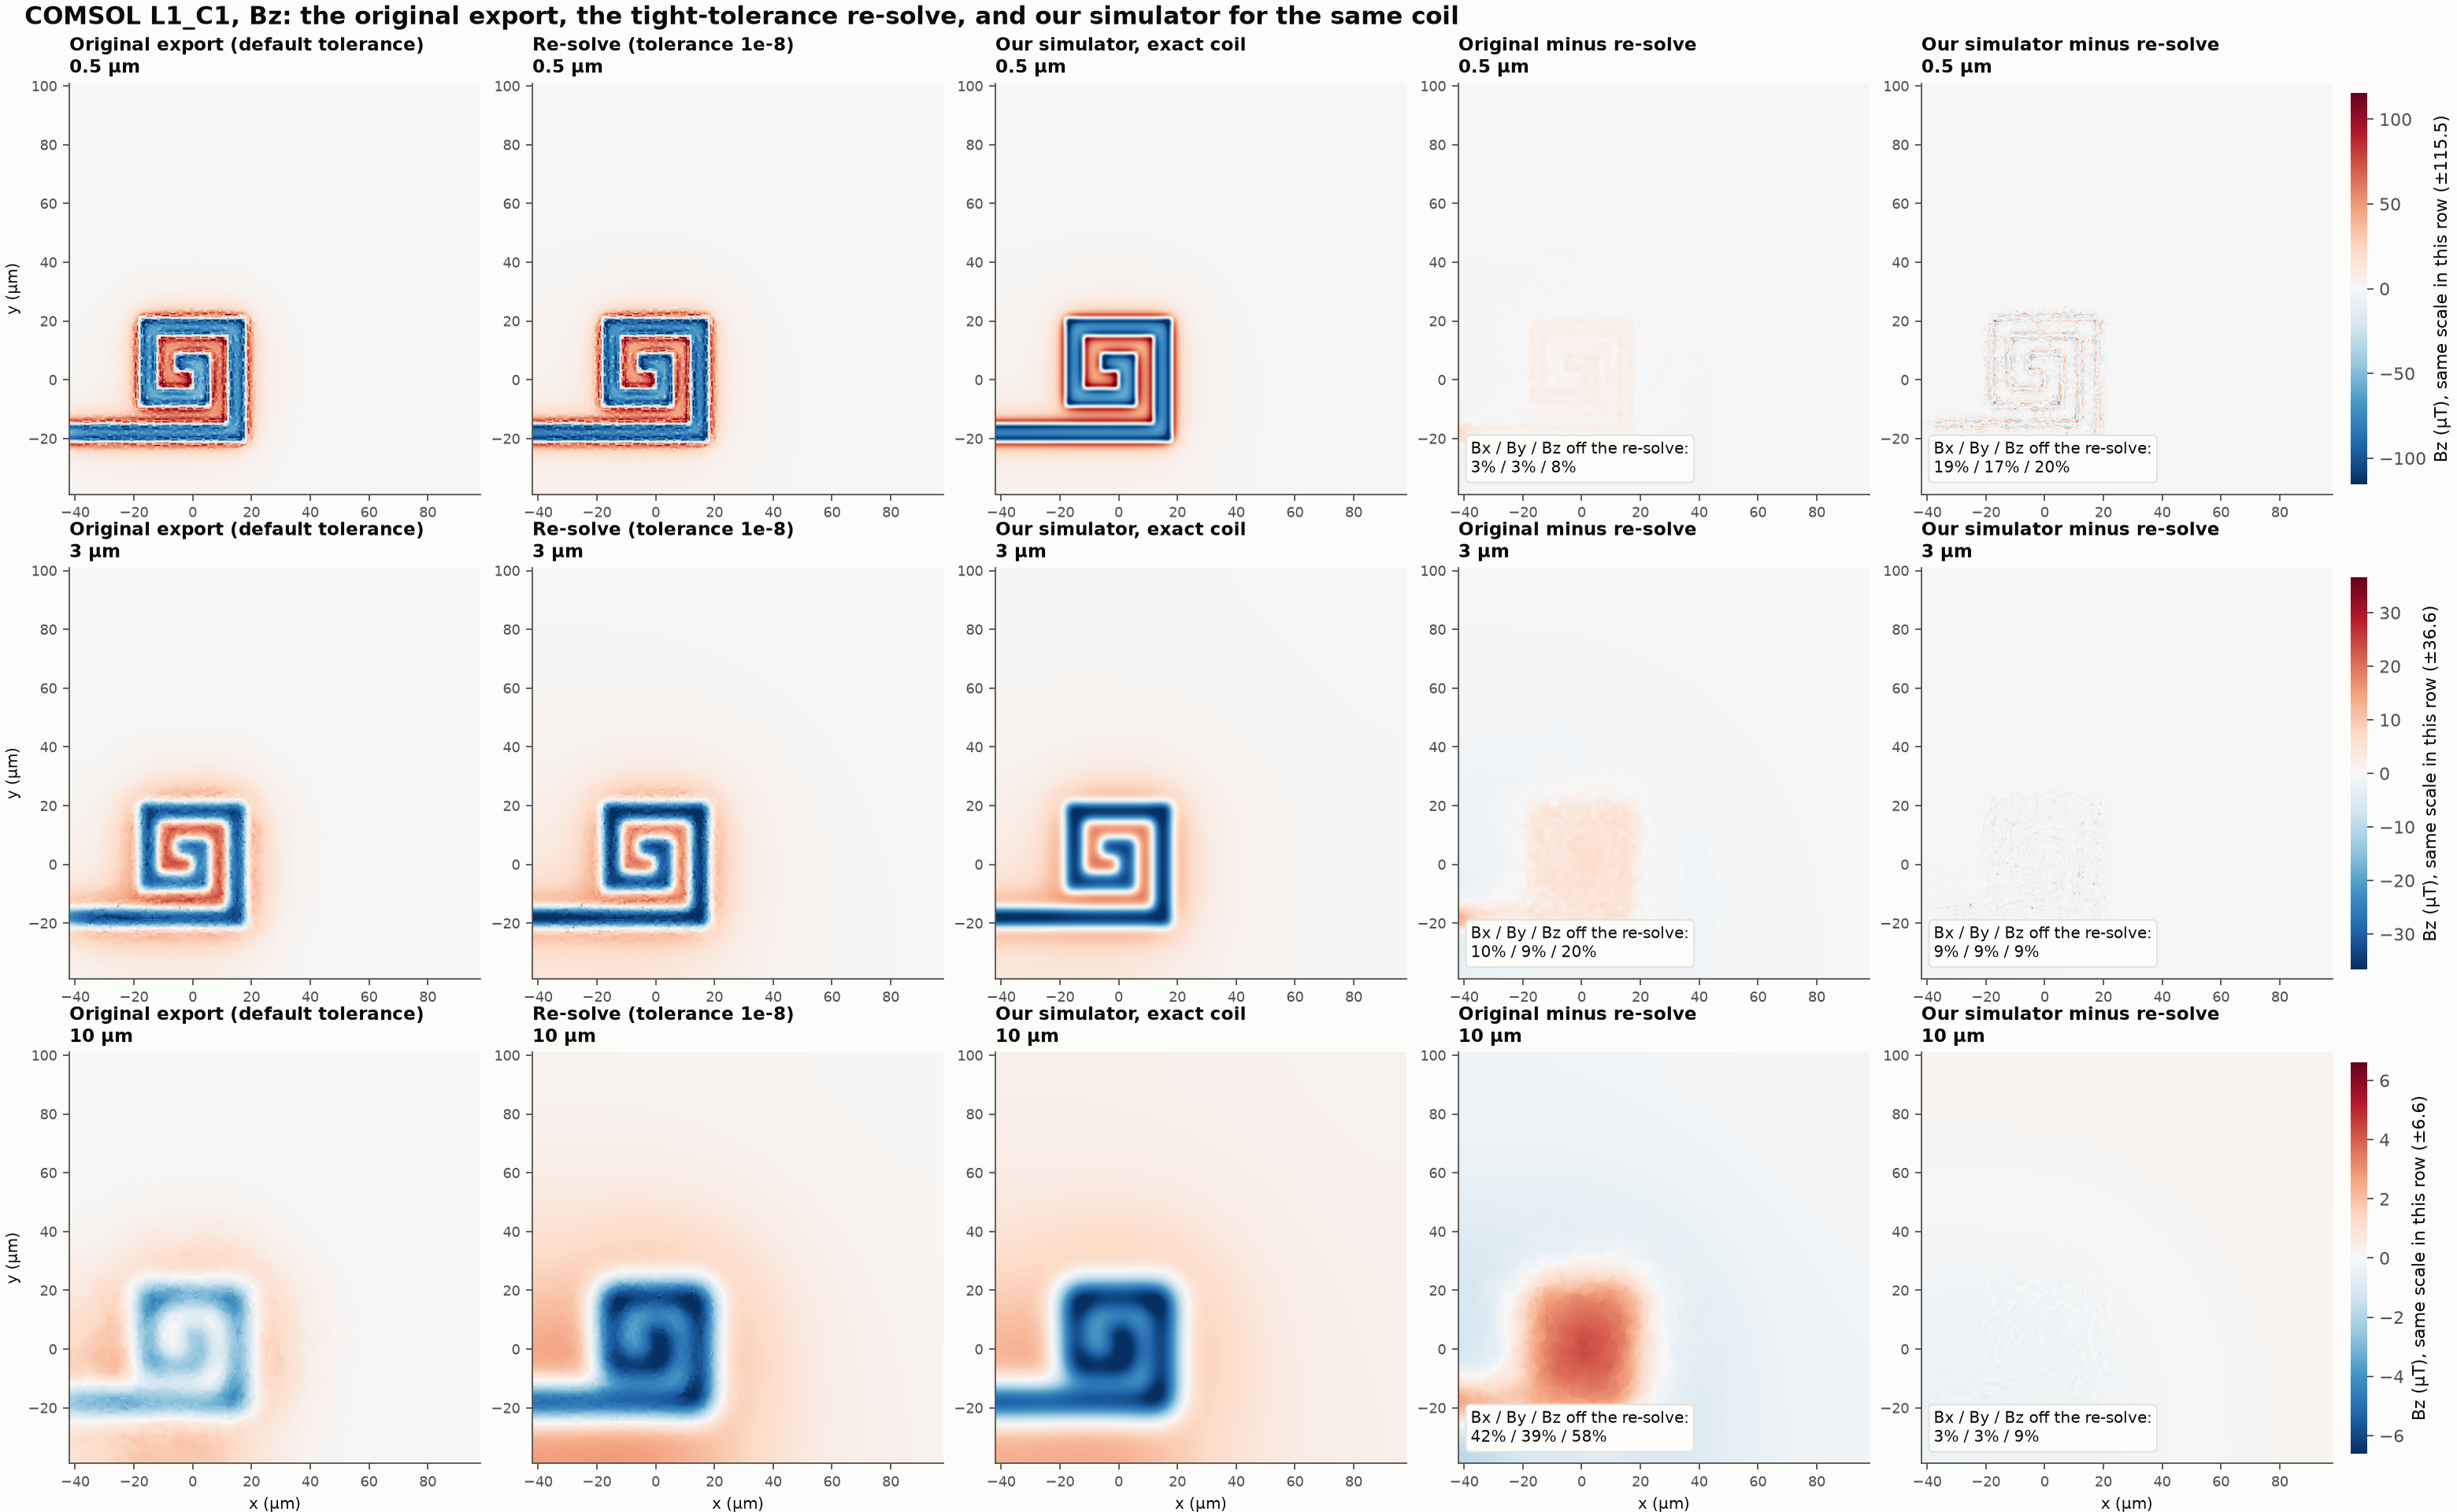
\includegraphics[width=\textheight]{cm_resolve_vs_old_maps}
\caption{$B_z$ of the three versions at 0.5, 3 and 10\um, and the differences from the re-solve. Each row has one colour
scale, so a lighter panel really is a weaker field.}
\label{fig:cm_three_maps}
\end{sidewaysfigure}

Read Figure~\ref{fig:cm_three_maps} row by row.
\begin{itemize}
\item \textbf{At 0.5\um} all three show the same spiral. The original and the re-solve differ by 3--8\%. Our simulator
differs from the re-solve by 17--20\%, but look at its difference panel: the error is a fine speckle along every wire
edge. That is COMSOL's mesh noise, which Chapter~\ref{ch:limits} measured at 14--18\% of the 0.5\um\ target. A clean
simulator cannot reproduce it, and should not.
\item \textbf{At 3\um} the original is already a little weak inside the coil (20\% off in $B_z$); our simulator is 9\%
off, again mostly speckle.
\item \textbf{At 10\um} the original has lost almost half its strength: its difference panel is one large smooth blob.
Our simulator's difference panel is nearly blank: 3 / 3 / 9\% off.
\end{itemize}

\begin{figure}[H]
\centering
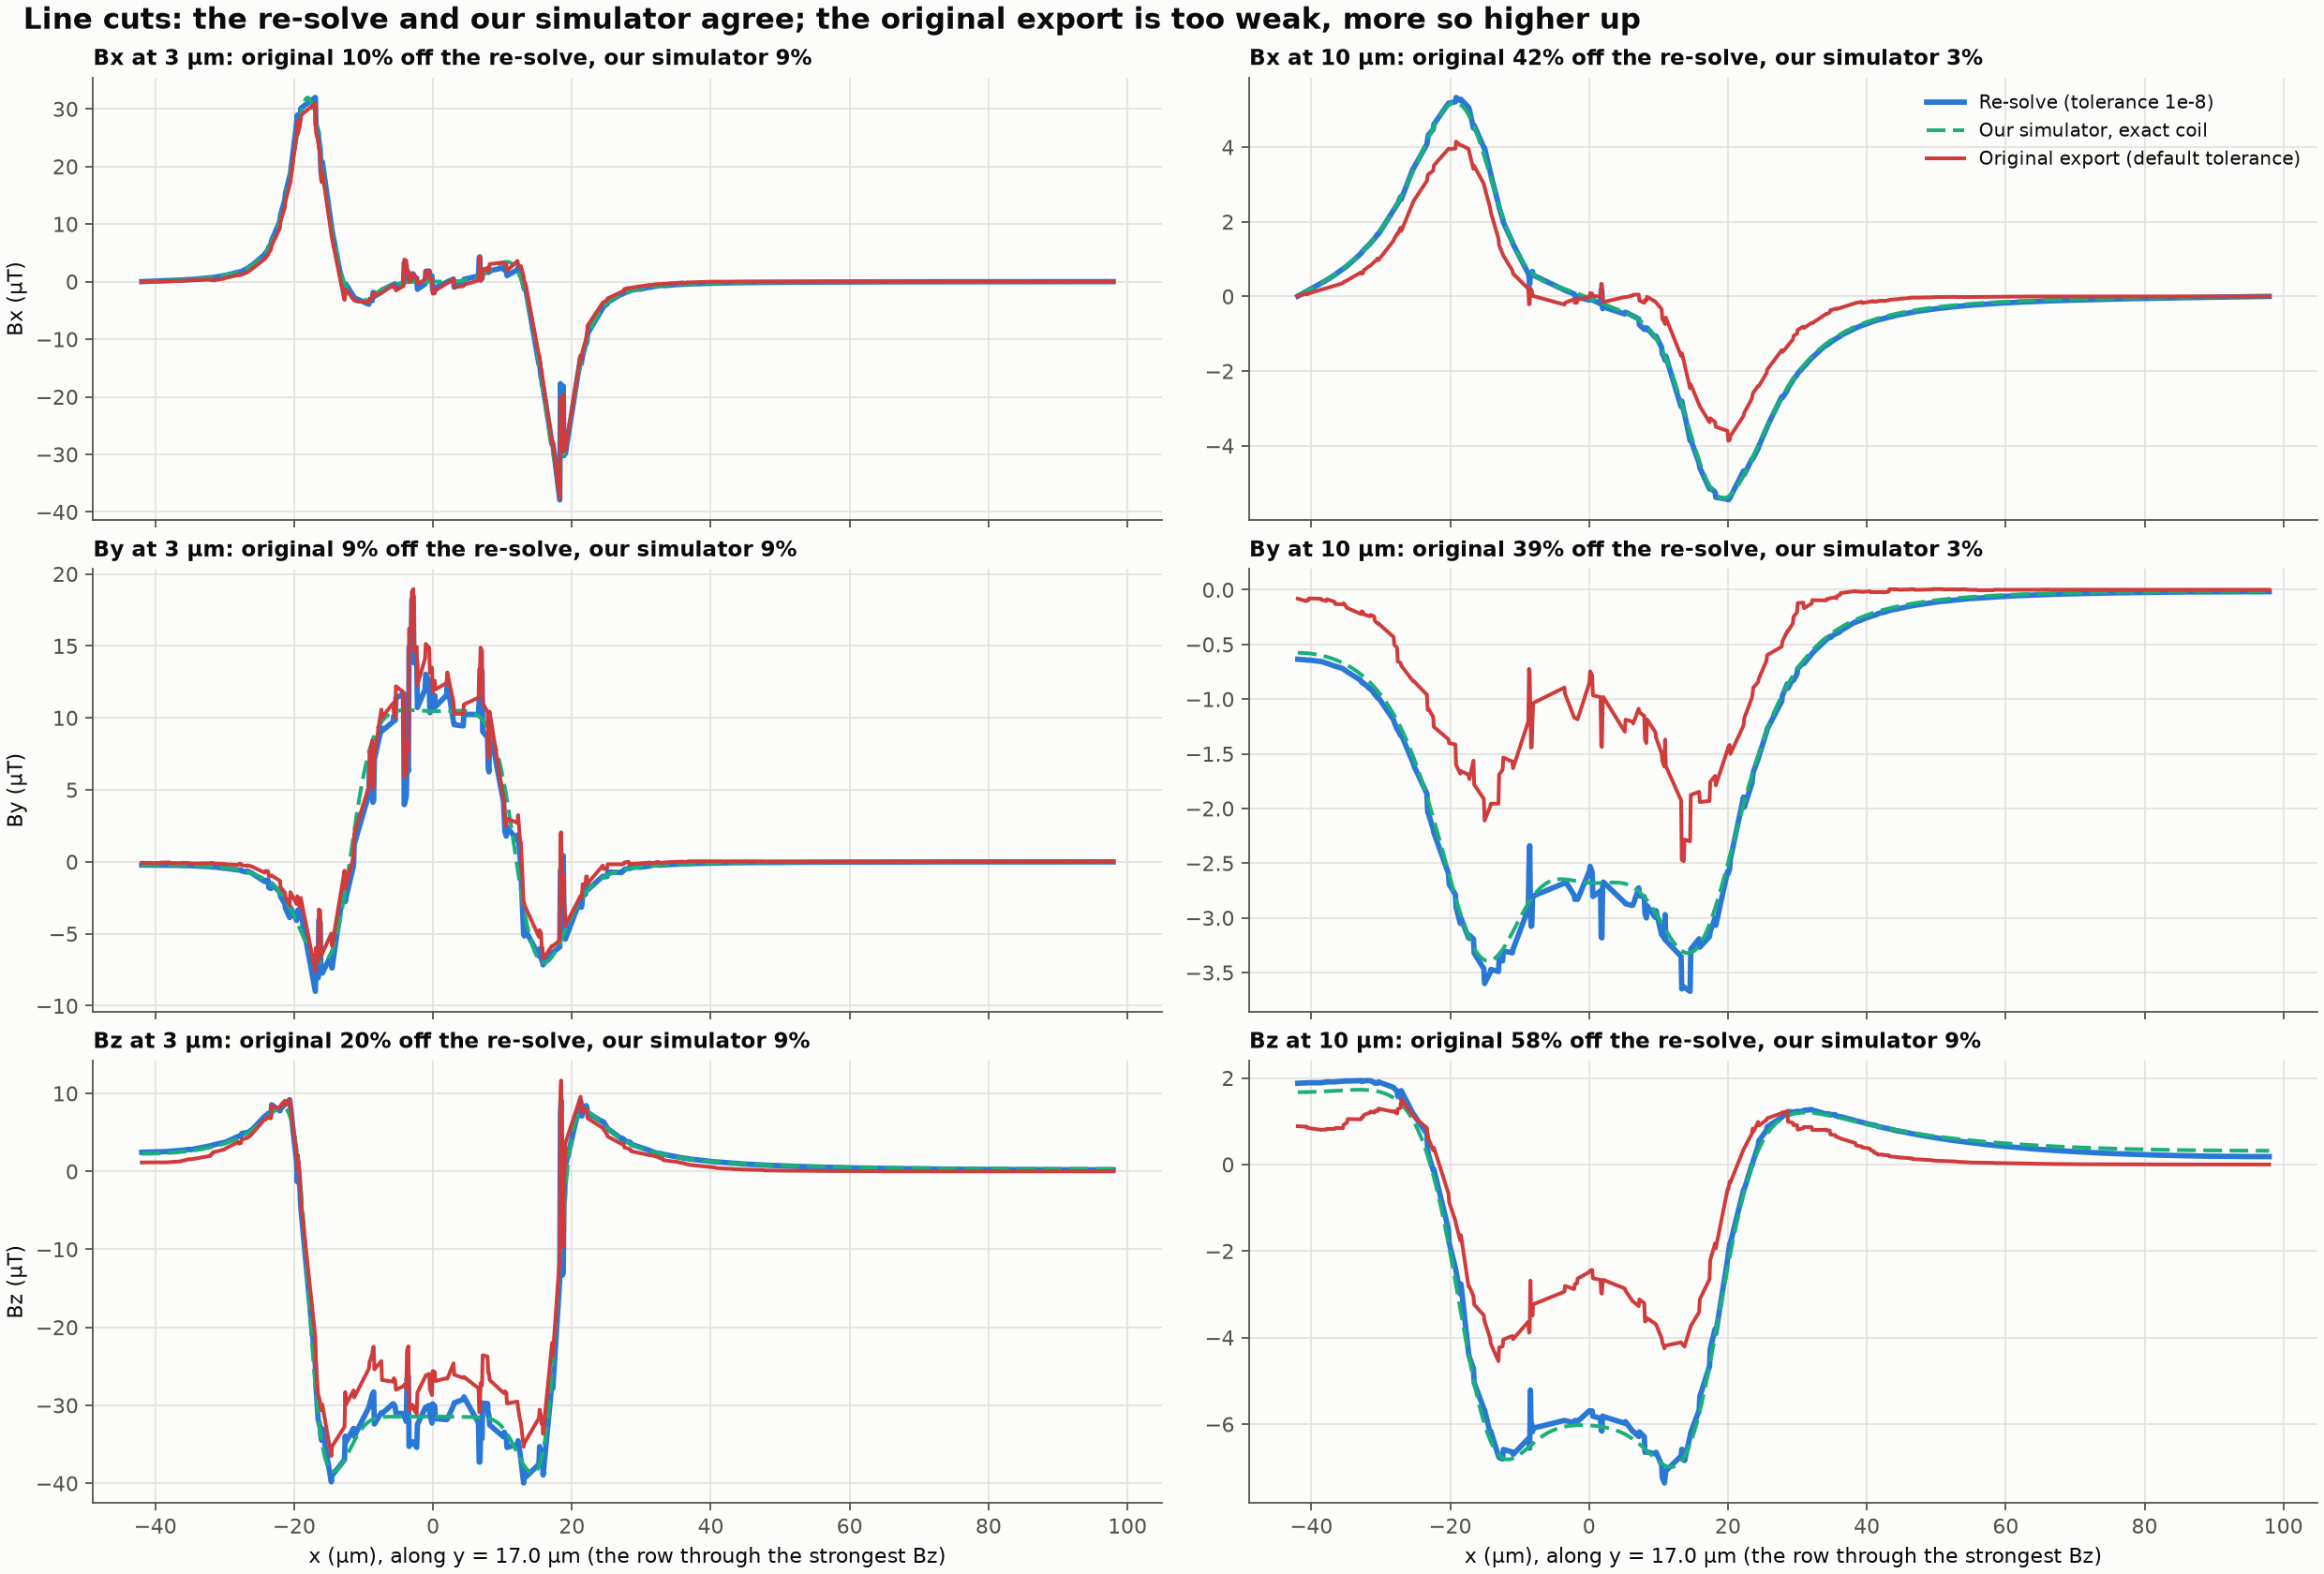
\includegraphics[width=\textwidth]{cm_resolve_vs_old_linecut}
\caption{A cut through the coil at 3\um\ (left) and 10\um\ (right), all three components. Blue: re-solve. Green
dashed: our simulator. Red: original export.}
\label{fig:cm_three_cuts}
\end{figure}

The line cuts make the point with no colour scale to argue about. At 3\um\ the three curves almost sit on each other.
At 10\um\ the green dashed line of our simulator lies on the blue re-solve, and the red original sits well inside both:
too weak, in every component.

\subsection*{Why an early-stopped solve damages exactly this}

COMSOL turns the physics into one enormous linear system, $A\mathbf{u}=\mathbf{f}$, with millions of unknowns. It does
not solve it in one go. An iterative solver starts from a guess and improves it step by step, and it stops once the
leftover mismatch is a small enough fraction of $\mathbf{f}$. That fraction is the tolerance.

Two facts then explain everything you see above.
\begin{enumerate}
\item \textbf{The error left behind is smooth.} Iterative solvers remove sharp, local errors quickly; broad, smooth
errors are the last to go. So when the solver stops early, what is left is a smooth error. In the field, smooth means
broad structure: low spatial frequencies $k$.
\item \textbf{Higher up, the field \emph{is} broad structure.} Fine detail decays as $e^{-kz}$, so the higher you go, the
more of what is left is broad. The right panel of Figure~\ref{fig:cm_three_why} measures it: the share of the field's
energy below $k=0.1$\,rad/\um\ is 2\% at 0.5\um, 11\% at 3\um\ and 68\% at 10\um.
\end{enumerate}
A smooth error is invisible near the coil, where almost nothing is broad, and dominant at 10\um, where almost everything
is.

\begin{sidewaysfigure}
\centering
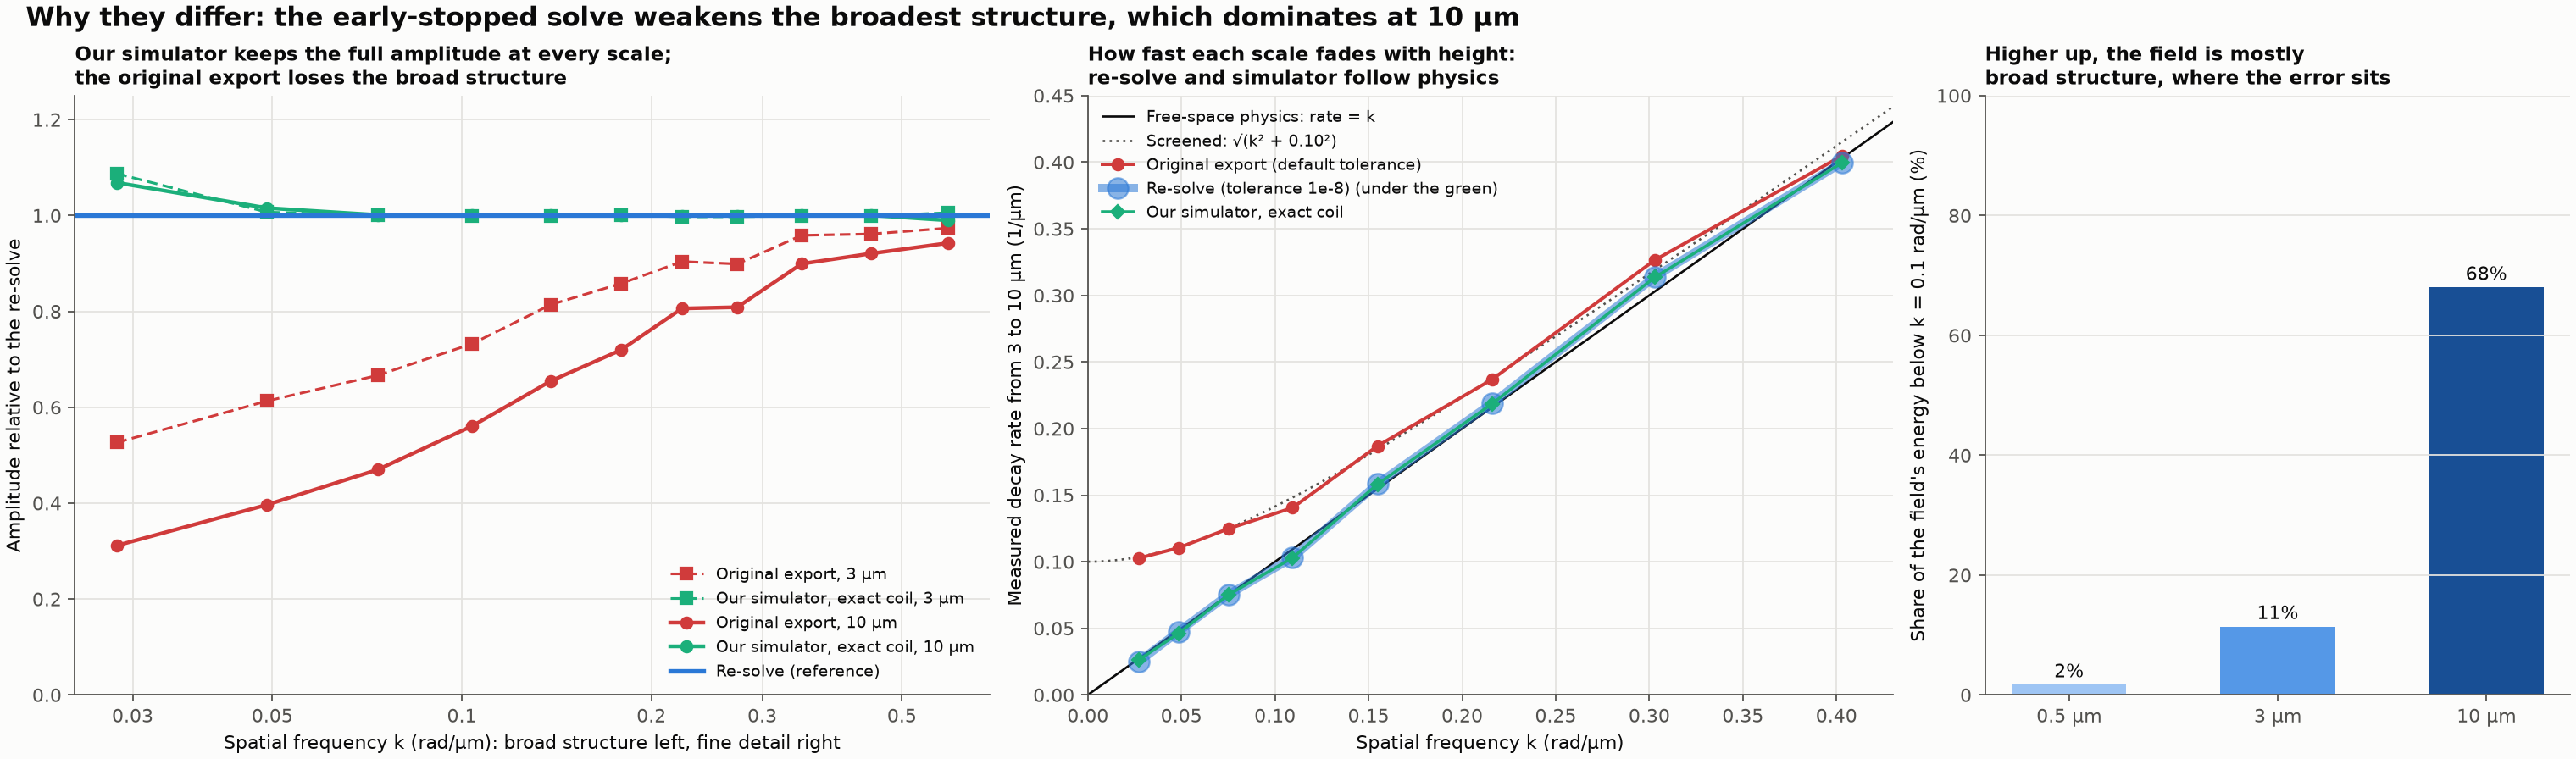
\includegraphics[width=\textheight]{cm_resolve_vs_old_why}
\caption{Left: amplitude of each version relative to the re-solve, per spatial frequency. Middle: how fast each
frequency fades between 3 and 10\um; free-space physics says the rate equals $k$. Right: how much of the field is broad
structure at each height.}
\label{fig:cm_three_why}
\end{sidewaysfigure}

\begin{itemize}
\item \textbf{Left:} the original export (red) keeps more than 90\% of the fine detail but only about 30\% of the broadest
structure at 10\um, and about 50\% at 3\um. Our simulator (green) stays at 1.0 at every scale; only the broadest band is
about 8\% high, where the coil's leads and the box walls matter most.
\item \textbf{Middle:} the original fades on the screened curve $\sqrt{k^2+0.10^2}$ of Section~\ref{sec:cm_decay}. The
re-solve and our simulator both fade at exactly $k$, as physics requires, and lie on top of each other.
\end{itemize}

\begin{center}
\small
\begin{tabular}{lccc}
\toprule
Off the re-solve ($B_x$ / $B_y$ / $B_z$) & 0.5\um & 3\um & 10\um \\
\midrule
Original export & 3 / 3 / 8\% & 10 / 9 / 20\% & 42 / 39 / 58\% \\
Our simulator, exact coil & 19 / 17 / 20\% & 9 / 9 / 9\% & \textbf{3 / 3 / 9\%} \\
\bottomrule
\end{tabular}
\end{center}

\begin{keyidea}[Where our simulator lies]
Next to the correctly solved field. Higher up, where COMSOL's mesh noise has decayed away, our simulator matches it to a
few per cent with nothing fitted. Near the coil the remaining difference is mostly mesh noise in COMSOL. The physics
used for every training set in this project was right; it was the old COMSOL export that was off.
\end{keyidea}

\begin{careful}[One modelling detail]
The figures close the coil's leads through the box walls, as COMSOL does. Our training layouts instead close every
loop with a rail outside the image. With plain zero padding and the leads simply ending at the image edge, the
simulator is 7 / 15 / 25\% off the re-solve at 10\um: the missing return current adds a field near the edge. That is a
statement about how this coil's leads are modelled, not about the physics.
\end{careful}

\textbf{What it changed for the results.} Every COMSOL score at 10\um\ in Chapter~\ref{ch:ten_results} used the original
export as input. On the re-solved \code{L1_C1}, MAGIC-UNet's 10\um\ error falls from 60.4\% to 26.2\%
(Section~\ref{sec:resolved}).

\begin{defend}[If your professor asks: why trust the re-solve and not the original?]
Because three independent checks agree with it and not with the original: it fades at exactly the free-space rate, it
satisfies Amp\`ere's law in empty air on a single plane, and it matches our simulator of the exact coil to 3--9\% at
10\um\ with nothing fitted. The original fails all three, and the only thing changed between them is the solver
tolerance.
\end{defend}

\begin{defend}[If your professor asks: how can you say COMSOL is wrong?]
COMSOL is not wrong; its default solver setting was too loose for the weak far field, and the re-solve with a tight
tolerance agrees with free-space physics to a few per cent. Before the re-solve: not wrong everywhere: near the coil it is fine, and at 3\um\ the effect is a few per cent in the measured band. But
above about 4\um\ its field in the air violates Amp\`ere's law by 27--52\%, where exact physics gives 1\% in the same
test. Empty air cannot carry current. Our simulator matches an independent Biot--Savart calculation to under 1\%, and
matches COMSOL to 10--12\% at every height once this one term is added.
\end{defend}

\begin{defend}[If your professor asks: why not just add $k_0$ and match the data?]
Because it would teach the network something that is not true of a real measurement. Chapter~\ref{ch:ten_results} shows
what the term does to a network trained without it: tens of points. A network trained \emph{with} it would lose those
points on a real instrument instead.
\end{defend}

\chapter{Ten micrometres: designing the run}\label{ch:ten}

Everything so far went from 3\um\ to 0.5\um. A real QDM often sits further from the sample. The last question of the
project was: can the 0.5\um\ field be reconstructed from a measurement at \textbf{10\um}? This chapter is about the
design, and the next about the results. The full record with every table is \code{README_HIGH_STANDOFF.md}, in the phase 9 folder of
\code{final_evaluation/02_source_docs}.

\section{Why 10\um\ is a different problem}

The blur is $e^{-k\,\Delta z}$, and now $\Delta z=9.5$\um\ instead of 2.5.

\begin{center}
\begin{tabular}{lcc}
\toprule
A pattern that repeats every & keeps, over 2.5\um & keeps, over 9.5\um \\
\midrule
40\um & 68\% & 22\% \\
10\um & 21\% & 0.3\% \\
4\um & 2\% & $3\times10^{-7}$ \\
\bottomrule
\end{tabular}
\end{center}

\begin{figure}[H]
\centering
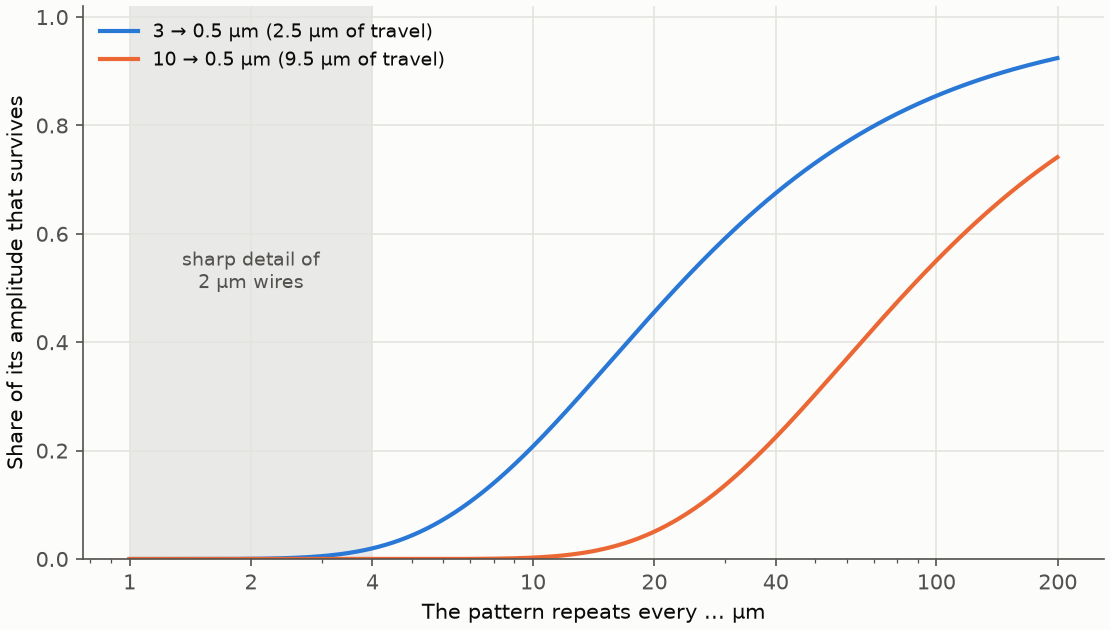
\includegraphics[width=0.75\textwidth]{late_decay}
\caption{How much of each pattern survives the blur, for the two problems. Wires 2\um\ wide have most of their sharp detail
far to the right of what survives at 10\um.}
\label{fig:late_decay}
\end{figure}

At 3\um\ a wire edge is weakened. At 10\um\ it is gone. On the COMSOL coils, 56\% (\code{L1_C1}) and 73.5\%
(\code{IC_4um}) of the 0.5\um\ field's norm lies where the 10\um\ measurement carries nothing (Chapter~\ref{ch:floor}). In
the language of Chapter~\ref{ch:limits}: the measured band has shrunk to almost nothing and nearly everything is prior
band. A method that only inverts the blur is stuck near 56--73\%. Only knowledge of what sources look like can do
better.

The existing networks do not reach. On simulated images at 10\um, run 2 scores 92\% and run 3 scores 56.8\%.

\section{How MAGIC-UNet sees a large image}

To understand the design you first need a piece of code that this booklet has not shown yet. The network only accepts
$64\times64$ images. A full image is $1400\times1400$. So it is cut into overlapping tiles, each tile is processed
alone, and the results are stitched.

Where the tiles start:

\begin{code*}{magic_unet.py}
def tile_starts(size, tile, stride):
    starts = list(range(0, size - tile + 1, stride))
    if starts[-1] != size - tile:
        starts.append(size - tile)
    return starts
\end{code*}

With a stride smaller than the tile, neighbours overlap. In the overlap, two tiles have each made a prediction. Which
one is kept? Each pixel goes to the tile whose \emph{centre} is nearest, because a network is most reliable in the middle
of its view and least at the edges:

\begin{code*}{magic_unet.py}
    pos = np.arange(size)[:, None]
    s = np.asarray(starts)[None, :]
    covers = (pos >= s) & (pos < s + tile)
    dist = np.where(covers, np.abs(pos - (s + (tile - 1) / 2)), np.inf)
    return np.asarray(starts)[dist.argmin(1)]
\end{code*}

And each tile is scaled by its own largest field before it enters the network, and scaled back afterwards:

\begin{code*}{magic_unet.py}
        x = torch.stack([full[:, r:r + tile, c:c + tile] for r, c in part])
        a = alpha(x).clamp_min(1e-30)
        y = model((x / a[:, None, None, None]).to(device)).cpu().double()
        y = y * a.double()[:, None, None, None] / beta
\end{code*}

\begin{keyidea}[The one fact that matters for 10\um]
Each tile is processed \textbf{alone}. The network sees 64 pixels by 64 pixels of field and nothing else. Whatever lies
outside that window does not exist for it.
\end{keyidea}

\section{The tile is too small at 10\um}

With 0.2\um\ pixels a tile is 12.8\um\ wide. At 3\um\ that is about four standoffs. At 10\um\ it is \emph{narrower than the
blur itself}, which is 15--20\um\ wide. The field inside such a tile is made mostly by wires that are not in it.

This can be measured with no network at all. Take a simulated layout. Keep only the current inside one tile and compute
its field. Compare with the field of the whole layout, inside the same tile. The difference is the part that comes from
outside:

\begin{code*}{tile_context_check.py}
            mx, my = np.zeros_like(jx), np.zeros_like(jy)
            mx[r:r + n, c:c + n], my[r:r + n, c:c + n] = jx[r:r + n, c:c + n], jy[r:r + n, c:c + n]
            inside = biot_savart_sheet(mx, my, dx, z)
            num = sum(np.sum((full[z][k][r:r + n, c:c + n] - inside[k][r:r + n, c:c + n]) ** 2) for k in range(3))
            den = sum(np.sum(full[z][k][r:r + n, c:c + n] ** 2) for k in range(3))
            out[(z, w)].append(np.sqrt(num / den))
\end{code*}

\code{mx, my} is the current with everything outside the tile set to zero. \code{full} is the field of the whole layout.
The last line is the share of the tile's field that the tile's own current cannot explain.

\begin{center}
\begin{tabular}{llc}
\toprule
Standoff & Tile & Share of the tile's field from currents outside it \\
\midrule
3\um\ (run 2) & 12.8\um & 50\% \\
8\um & 12.8\um & 70\% \\
10\um & 12.8\um & \textbf{78\%} \\
10\um & 25.6\um & 60\% \\
10\um & 44.8\um & \textbf{52\%} \\
\bottomrule
\end{tabular}
\end{center}

Each number is the median over 12 tiles from 4 layouts, and single tiles vary widely (for example 48--123\% at 10\um\ with
the small tile), so read the trend, not the digits. At 10\um\ with the old tile, four fifths of what the network sees was made by something it cannot see. A 44.8\um\ tile
brings the share back to run 2's.

\begin{figure}[H]
\centering
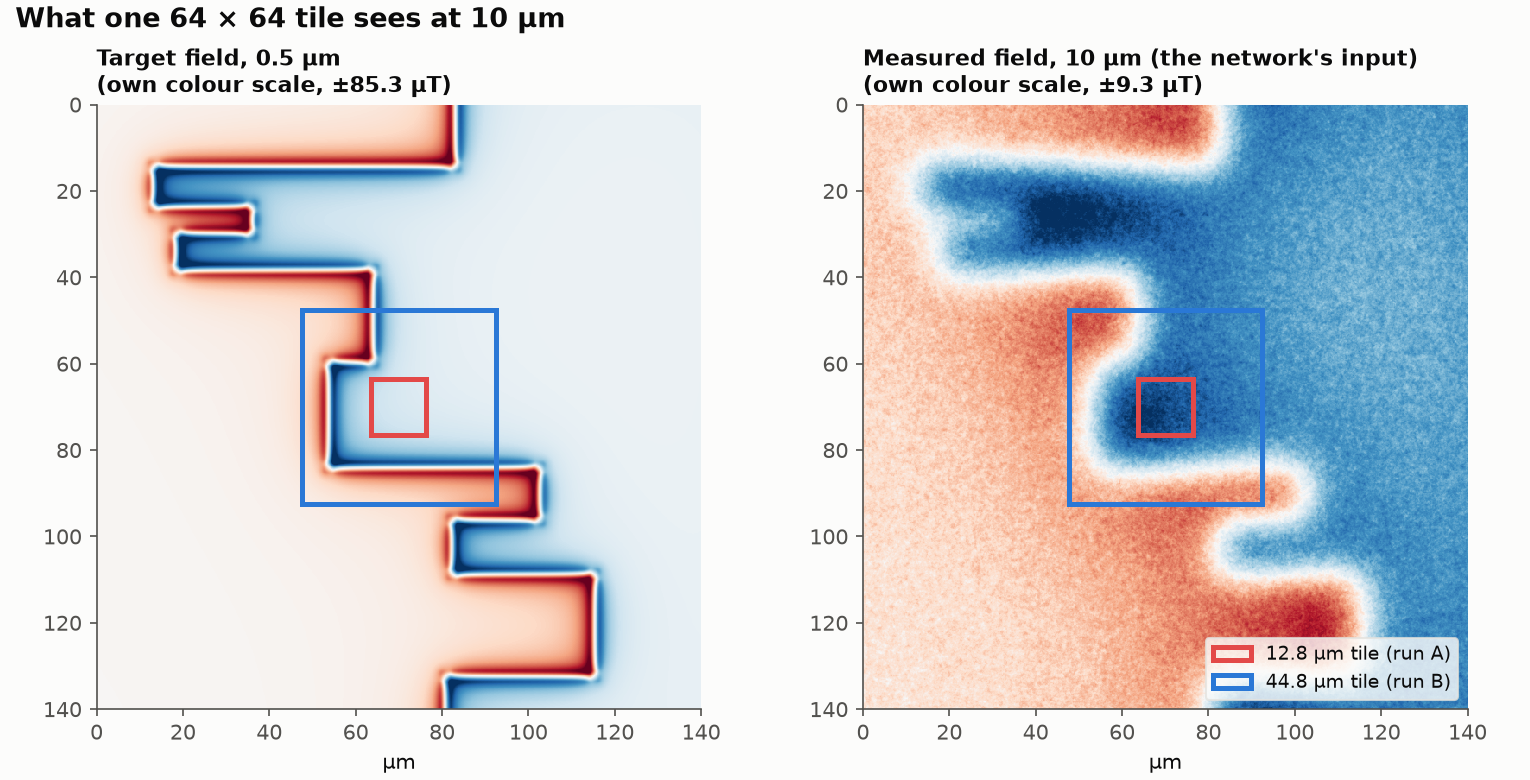
\includegraphics[width=0.92\textwidth]{hs_tile_context}
\caption{The target at 0.5\um\ and the measured field at 10\um\ for one test layout, with both tile sizes drawn on them.
Inside the small tile the measured field is almost featureless.}
\label{fig:hs_tiles}
\end{figure}

\section{Bigger pixels, not a bigger network}

How do you make a 44.8\um\ tile without changing the network? The network must stay $64\times64$: you asked for the
paper's architecture, unmodified. So keep 64 pixels and make each pixel larger: $44.8/64=0.7$\um. The simulator works
at 0.1\um, so 7 by 7 of its pixels are averaged into one:

\begin{code*}{magic_data.py}
def binned(a, factor):
    """Area average over factor x factor pixels; a: [..., H, W]."""
    if factor == 1:
        return a
    *lead, h, w = a.shape
    return a.reshape(*lead, h // factor, factor, w // factor, factor).mean((-3, -1))
\end{code*}

Run 2 already did this with \code{factor = 2}. Averaging pixels is what a camera does when it bins.

At inference the same averaging is applied to the measured field, the network predicts a current on the coarse grid,
and the current is copied back onto the fine grid before the physics step:

\begin{code*}{train_magic_unet.py}
    j = predict_tiled(model, binned(np.asarray(b, np.float64), factor), beta, args.tile, stride,
                      args.infer_batch, device)
    j = np.kron(j, np.ones((1, factor, factor)))
    return field_from_sheet(j, height, DX), j
\end{code*}

\code{np.kron} with a block of ones repeats each coarse pixel $7\times7$ times. The score is then taken on the full
$1400\times1400$ image at 0.1\um, exactly as for every other method.

\begin{careful}[What bigger pixels cost]
A current drawn on 0.7\um\ pixels cannot have edges sharper than 0.7\um. Measured with a \emph{perfect} current and no
network: 2.2\% error with 0.2\um\ pixels, 3.1\% with 0.5\um, 4.6\% with 0.7\um. So run B starts 2.4 points behind before
it has learned anything. The bet was that seeing the wires is worth far more than that.
\end{careful}

\section{The standoff band}

Run 3 broke at 10\um\ because 10\um\ was the \emph{edge} of its range (Chapter~\ref{ch:run3}). So the new runs put 10\um\ in
the middle: a normal distribution around 10\um\ with a spread of 2\um, cut at three spreads, which gives 4 to 16\um. It is
the same 20\% spread as run 2's $3\pm0.6$\um\ (and as our reading of the paper's $50\pm10$\um), and it uses the code path of
Chapter~\ref{ch:run3} with \code{--z-mean 10 --z-std 2}. As always, the network is never given the value.

\section{Two runs that differ in one thing}

\begin{center}
\begin{tabular}{lcc}
\toprule
 & Run A (control) & Run B \\
\midrule
Training standoff & \multicolumn{2}{c}{$10\pm2$\um, never given to the network} \\
Pixels & 0.2\um\ (\code{--bin 2}) & 0.7\um\ (\code{--bin 7}) \\
Tile & 12.8\um & 44.8\um \\
Training crops & \multicolumn{2}{c}{4{,}800 layouts $\times$ 4 standoffs $\times$ 8 crops $=$ 153{,}600} \\
Network and recipe & \multicolumn{2}{c}{unmodified, the paper's: RMSprop, $10^{-4}$, 50 epochs, batch 32} \\
\bottomrule
\end{tabular}
\end{center}

Run A is run 2 with only the standoff changed. Run B is run A with only the pixel size changed. If B beats A, the
pixel size is the reason, and nothing else can be.

\begin{careful}[What is ours here]
The network and the training recipe are the paper's. The two pixel sizes and the split into 4{,}800 layouts with 8 crops
per standoff are our choices. Run 2 used 2{,}400 layouts with 16 crops per standoff; the total number of crops is the
same, 153{,}600.

The pixel-size change was made for MAGIC-UNet only. When CSC-LISTA and FISTA-Net were later run at 10\um, they kept
their 3\um\ settings, so the 10\um\ method comparison is not like-for-like (Section~\ref{sec:fair}).
\end{careful}

\section{The rules, written first}

As in Chapter~\ref{ch:fista_depth}, the rules were fixed and hashed before either run was launched. They are in
the file \code{HIGH_STANDOFF_PROTOCOL.md}:
\begin{itemize}
\item \textbf{Main test:} 50 held-out \emph{simulated} layouts at 10\um, scored at full resolution. The same layouts at 6, 8,
12 and 14\um\ show the range.
\item \textbf{Second test:} the 15 COMSOL pairs at 10\um. Nothing is chosen on them, and they are reported with the warning
of Chapter~\ref{ch:comsol}.
\item \textbf{A against B:} the lower simulated error wins; under one point is a tie.
\item \textbf{Baseline:} FISTA, with everything about it chosen on simulation.
\end{itemize}

\begin{keyidea}[Why the main test is simulation this time]
At 3\um\ COMSOL was a fair test and we kept it as the judge. At 10\um\ Chapter~\ref{ch:comsol} showed that COMSOL's field
is not the field a real coil would make. Judging a physically trained network by it would be judging it against an
artefact. So the judge is free-space simulation, on layouts the network has never seen, and COMSOL is shown beside it.
The re-solve of 17 November (Chapter~\ref{ch:comsol}) confirmed the choice: the 10\um\ COMSOL inputs that were scored
are 39--58\% away from a correctly solved field, while the free-space simulator matches the re-solve to 3--9\%.
\end{keyidea}

Six amendments followed, each dated and written before the number it affects: details of the FISTA baseline (A1 to A3),
a server crash and restart (A4), a check added afterwards (A5), and the other learned methods at 10\um\ (A6).

\section{A crash, and a bug that had never been run}

On 15 November the server ran out of memory and was rebooted. Run A had finished. Run B was killed during its last
epoch, with 49 of 50 saved. The trainer saves a checkpoint after every epoch and can continue from it:

\begin{code*}{train_magic_unet.py}
        state = torch.load(latest, map_location=device, weights_only=False)
        model.load_state_dict(state['model'])
        optimizer.load_state_dict(state['optimizer'])
\end{code*}

The first attempt to resume stopped at once. The checkpoint also stores the state of the random number generator, and
\code{map_location=device} had moved \emph{everything} in the file to the GPU, including that state, which PyTorch only
accepts on the CPU. One word fixed it:

\begin{code*}{train_magic_unet.py}
        torch.set_rng_state(state['torch_rng'].cpu())      # map_location moved it to the GPU
\end{code*}

\begin{careful}[The lesson]
The restart path had existed since run 2 and had never once been used on the GPU. Code that has never run is code
that does not work yet. The fix does not touch training or scoring, and it is recorded in amendment A4. One honest
detail: after the restart the last epoch drew different training noise than an uninterrupted run would have.
\end{careful}

\begin{defend}[If your professor asks: did you change the network for 10\um?]
No. It is the same 15{,}505{,}194 parameters and the same training recipe. What changed is the data: the standoff
band, and the pixel size, so that 64 pixels cover 44.8\um\ instead of 12.8\um. Both are labelled as our choices.
\end{defend}

\begin{defend}[If your professor asks: why 0.7\um\ pixels and not some other number?]
Because of a measurement made before training. At 10\um\ a 12.8\um\ tile gets 78\% of its field from wires outside it; a
44.8\um\ tile gets 52\%, the same as run 2 had at 3\um. 44.8\um\ over 64 pixels is 0.7\um. And we ran the 0.2\um\ version too,
as the control, so the claim rests on a comparison and not on the argument.
\end{defend}

\chapter{Ten micrometres: the results}\label{ch:ten_results}

In every comparison of this chapter, \textbf{MAGIC-UNet} means run B (0.7\um\ pixels, 44.8\um\ tile) with the
data-consistency step of Chapter~\ref{ch:consistency} at the height the network itself estimates. Run A appears only
where the tile size is the subject.

\section{On simulation}

\begin{center}
\begin{tabular}{lcc}
\toprule
Simulation, 10\um\ to 0.5\um & Error & Layouts \\
\midrule
MAGIC-UNet & \textbf{15.8\%} & 50 \\
MAGIC-UNet, on the 20 layouts below & \textbf{14.7\%} & 20 \\
FISTA, 3{,}000 iterations & 48.8\% & 20 \\
CSC-LISTA, with its 3\um\ settings & 91.8\% & 20 \\
FISTA-Net & still training & \\
\bottomrule
\end{tabular}
\end{center}

MAGIC-UNet is better than FISTA on all 20 layouts. FISTA is told the standoff. MAGIC-UNet is not.

\begin{figure}[H]
\centering
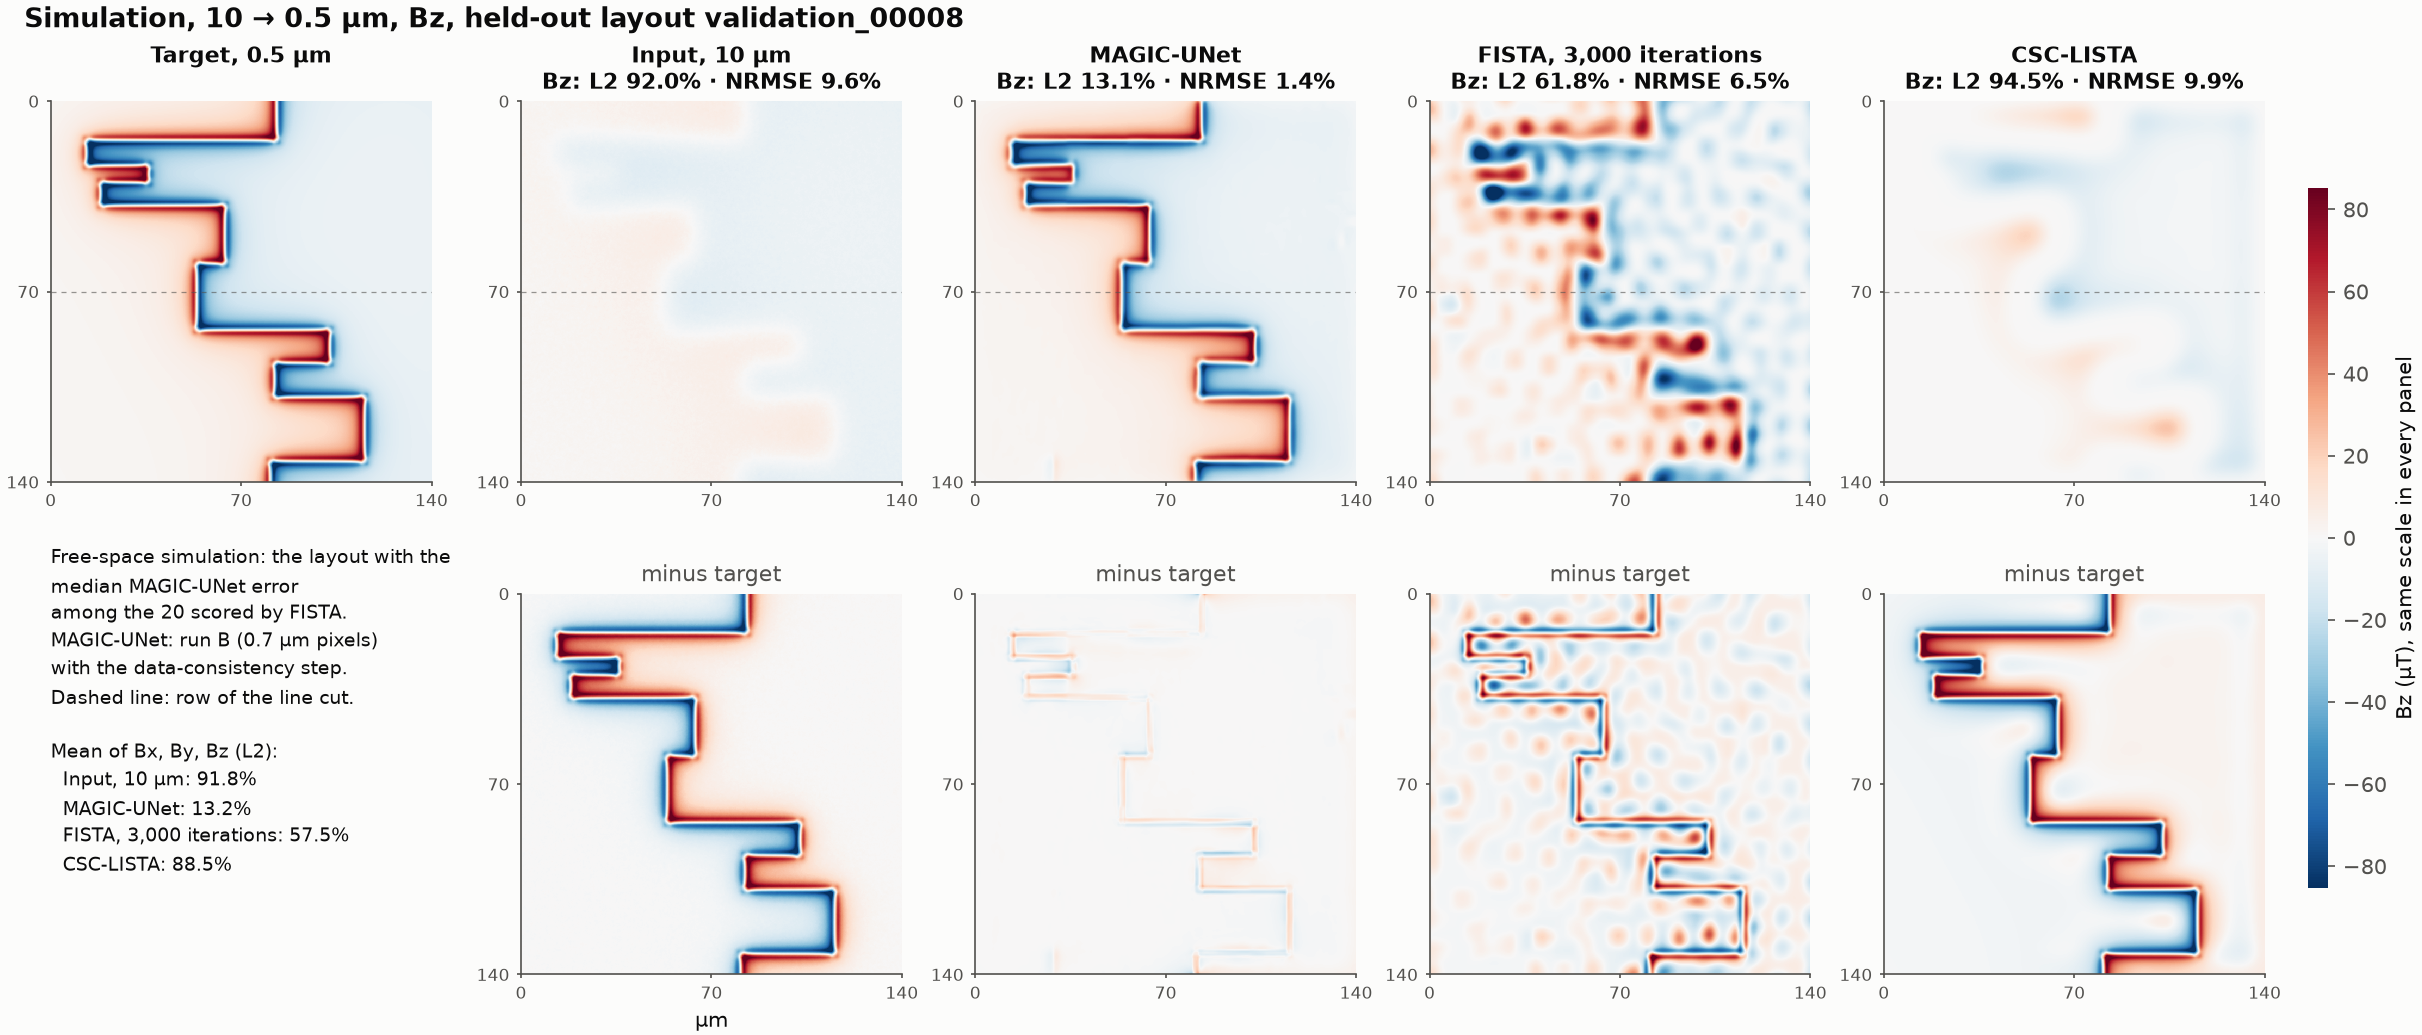
\includegraphics[width=\textwidth]{hs_sim_median_maps}
\caption{A held-out simulated layout, chosen by a rule: the one with the median MAGIC-UNet error among the 20 layouts.
Every panel uses the same colour scale, so the nearly blank second panel is the true size of the measured field. Bottom
row: output minus target.}
\label{fig:hs_sim}
\end{figure}

Look at what each method does in Figure~\ref{fig:hs_sim}. The measurement holds a faint, smooth shadow of the wire.
FISTA finds where the wire runs, but it can only rebuild what its dictionary and the measurement support, and the wire
comes out as a string of blobs. MAGIC-UNet draws a wire: a continuous path of constant width. It has learned that
currents come in wires, and it uses the shadow only to decide where the wire goes.

\begin{figure}[H]
\centering
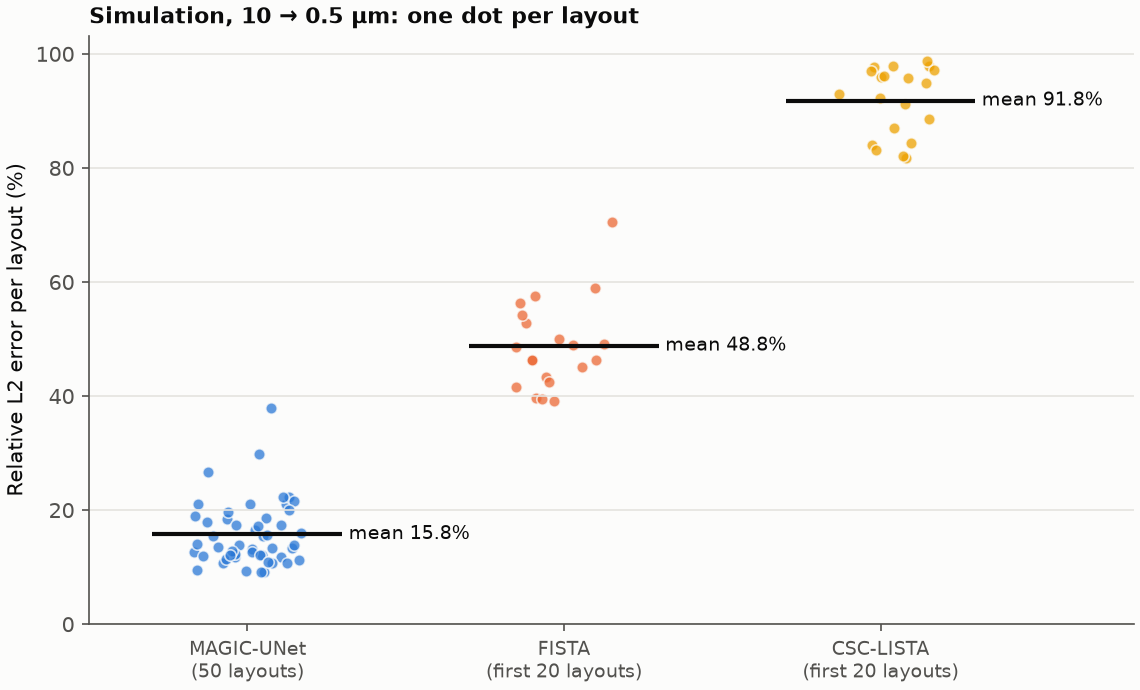
\includegraphics[width=0.7\textwidth]{hs_per_layout_10um}
\caption{One dot per layout at 10\um\ to 0.5\um.}
\label{fig:hs_dots}
\end{figure}

\begin{careful}[What 15.8\% is, and is not]
The test layouts are new, but they come from the same simulator as the training layouts: the same three families of
layout, wire widths of 1.6--3.2\um\ and one current of 600\,\textmu A. At 10\um\ nearly all of the 0.5\um\ field is prior
band (Chapter~\ref{ch:limits}), so nearly all of the output comes from what the network learned wires look like. That is
what a learned source prior is for. It is also its limit: nothing here says the number holds for other wire shapes or
several currents. The review's second risk, ``the prior has memorised the simulator'', is not answered by this test.
\end{careful}

\section{The tile size is what makes it work}

\begin{center}
\begin{tabular}{llcc}
\toprule
Model & Tile & Trained on & Simulation, 10\um\ to 0.5\um \\
\midrule
Run B & 44.8\um & $10\pm2$\um & \textbf{15.8\%} \\
Run A & 12.8\um & $10\pm2$\um & 58.2\% \\
Run 3 & 12.8\um & 1--10\um & 55.4\% \\
Run 2 & 12.8\um & $3\pm0.6$\um & 90.8\% \\
\bottomrule
\end{tabular}
\end{center}

Same network, same layouts, same recipe. With the small tile MAGIC-UNet is \emph{worse} than FISTA. With the large tile
it is three times better. Run B beats run A on all 50 layouts. The measurement of Chapter~\ref{ch:ten} had predicted the
direction before a single epoch was trained.

\begin{figure}[H]
\centering
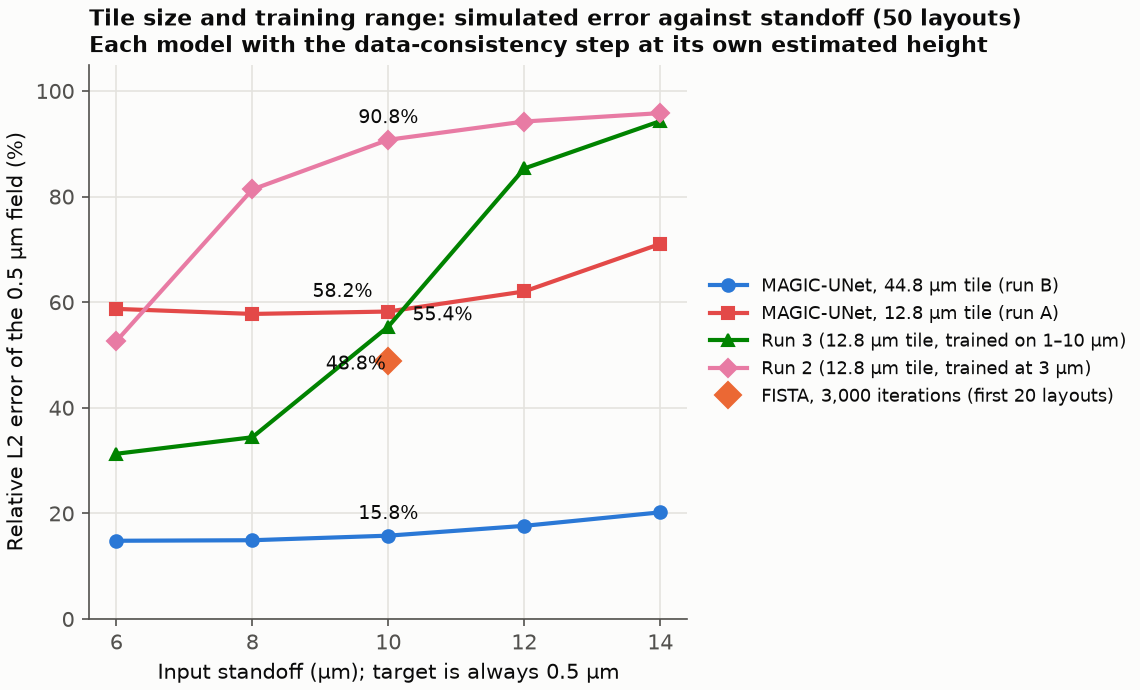
\includegraphics[width=0.85\textwidth]{hs_error_vs_standoff}
\caption{The same 50 layouts at input standoffs from 6 to 14\um. One run B model covers the whole range (14.8--20.2\%)
without being told the height.}
\label{fig:hs_standoff}
\end{figure}

\section{The height read-out and the correction at 10\um}

\begin{figure}[H]
\centering
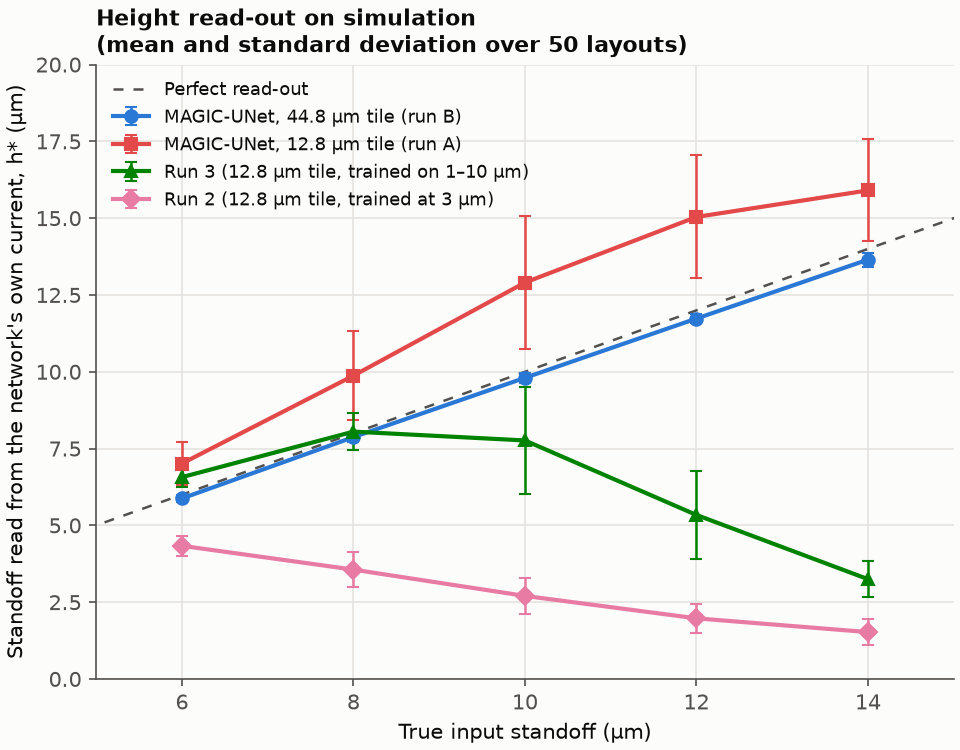
\includegraphics[width=0.6\textwidth]{hs_height_readout}
\caption{Standoff read from each network's own current (Chapter~\ref{ch:height}) against the true standoff.}
\label{fig:hs_height}
\end{figure}

Run B reads 9.80\um\ at a true 10\um, and is within 0.14--0.39\um\ from 6 to 14\um. Run A reads 12.9\um. This is
Chapter~\ref{ch:height} again: the read-out is as good as the current it is read from.

\begin{center}
\begin{tabular}{lcccc}
\toprule
 & Raw & Corrected, true height & Corrected, $h^\ast$ & Best $\mu$ at 10\um \\
\midrule
Run B & 16.3\% & 15.8\% & 15.8\% & 0.178 \\
Run A & 54.8\% & 50.8\% & 58.2\% & 0.0032 \\
\bottomrule
\end{tabular}
\end{center}

Two things to learn from this table.
\begin{itemize}
\item \textbf{For run B the correction hardly matters.} The selection picked a large $\mu$, which means ``leave the network
alone''. Remember the dial $w$ of Chapter~\ref{ch:consistency}: at 10\um\ the measurement only reaches the lowest
frequencies (Figure~\ref{fig:late_dc}, right), and there run B already agrees with it.
\item \textbf{For run A the correction hurts.} At the true height it would help. But run A's height is 3\um\ too high, and a
correction built on a wrong height amplifies in the wrong place. A data-consistency step is only as good as the
height it is given.
\end{itemize}

\section{The FISTA baseline at 10\um}

Everything about FISTA was chosen again on simulated data at 10\um.
\begin{itemize}
\item \textbf{Padding.} The blur is much wider now, so more zero padding might be needed. Tested at 128, 256, 384 and 512
pixels: 63.2, 63.6, 63.9 and 64.0\%. More padding does not help, so 128 stays.
\item \textbf{Penalty.} The best $\lambda$ is thirty to a hundred times smaller than at 3\um.
\item \textbf{Depth.} From the curve of Chapter~\ref{ch:fista_depth}, recorded every 25 iterations.
\end{itemize}

\begin{figure}[H]
\centering
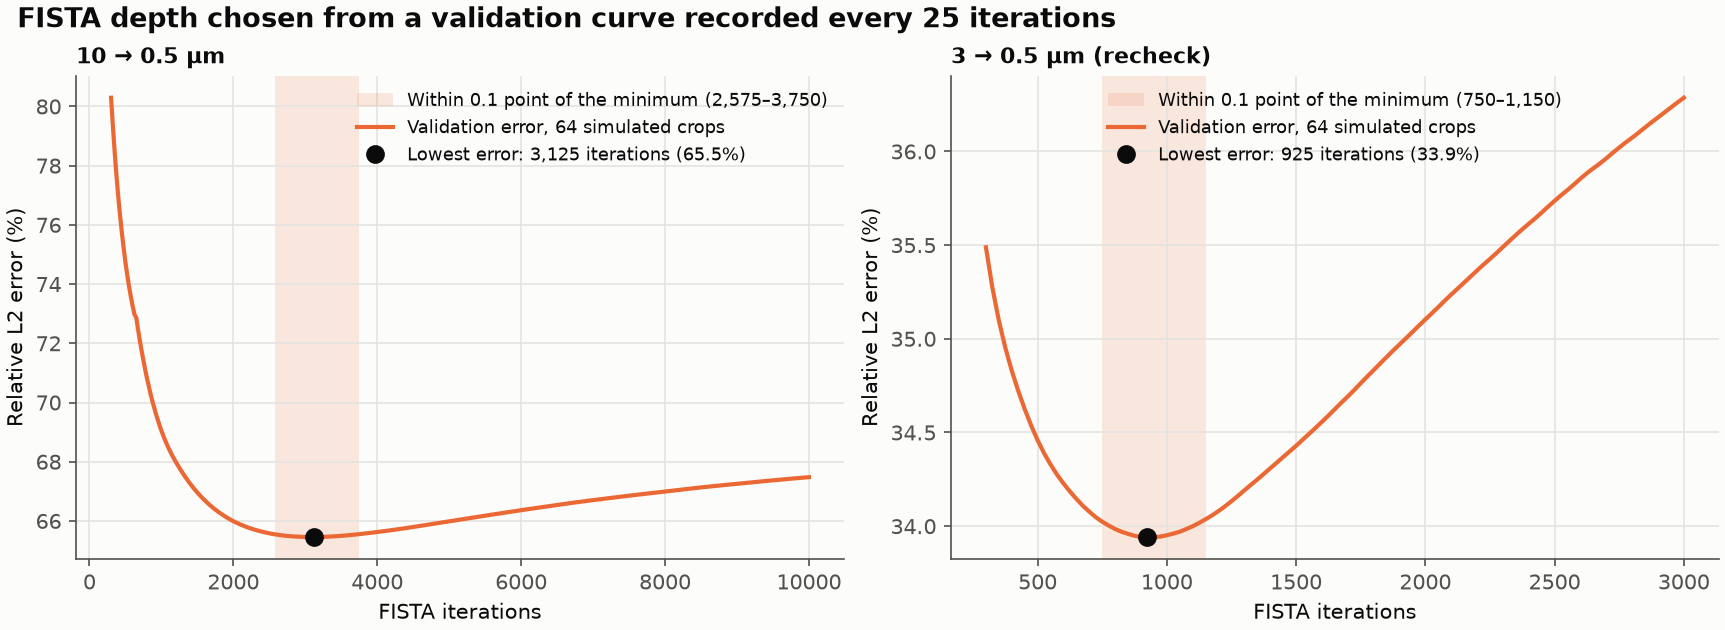
\includegraphics[width=\textwidth]{hs_fista_depth_curves}
\caption{FISTA's error on 64 simulated validation crops against the number of iterations. The dot marks the lowest
error; the band marks every depth within 0.1 points of it.}
\label{fig:hs_fista}
\end{figure}

The first curve ended at 3{,}000 iterations, which was then its lowest point. So the minimum might lie beyond. It was
extended to 10{,}000. The minimum is at \textbf{3{,}125} iterations: 65.46\%, only 0.004 points below the value at
3{,}000, and the curve rises slowly afterwards (67.5\% at 10{,}000). The rule written beforehand asked for a gain of
half a point before re-scoring, so FISTA at 3{,}000 stays the baseline. It is now known to sit at the minimum.

\begin{keyidea}[925 at 3\um, 3{,}125 at 10\um]
FISTA needs more than three times as many iterations at 10\um. The reason is in the gradient step. The step size is
set by the \emph{strongest} frequency the blur lets through. A frequency that the blur weakens by a factor $H$ is then
corrected $H^2$ times more slowly. At 10\um\ the useful frequencies are weakened far more, so they need far more steps.
\end{keyidea}

(The 64-crop curve reads 65\% and the full-image score is 48.8\%. A 51\um\ crop loses the surrounding field that a full
140\um\ image keeps. The full-image number is the one compared with MAGIC-UNet.)

\section{On COMSOL}

\begin{center}
\begin{tabular}{lccc}
\toprule
COMSOL, 10\um\ to 0.5\um & 15 pairs & C1 family & \code{IC_4um} \\
\midrule
FISTA, 3{,}000 iterations & \textbf{54.3\%} & \textbf{50.2\%} & 71.0\% \\
MAGIC-UNet & 59.3\% & 59.6\% & \textbf{58.3\%} \\
CSC-LISTA, with its 3\um\ settings & 98.1\% & 99.6\% & 92.4\% \\
FISTA-Net & \multicolumn{3}{c}{still training} \\
\bottomrule
\end{tabular}
\end{center}

On COMSOL the order flips. FISTA is ahead on the mean and on the C1-family coils. MAGIC-UNet is ahead on
\code{IC_4um}.

\begin{figure}[H]
\centering
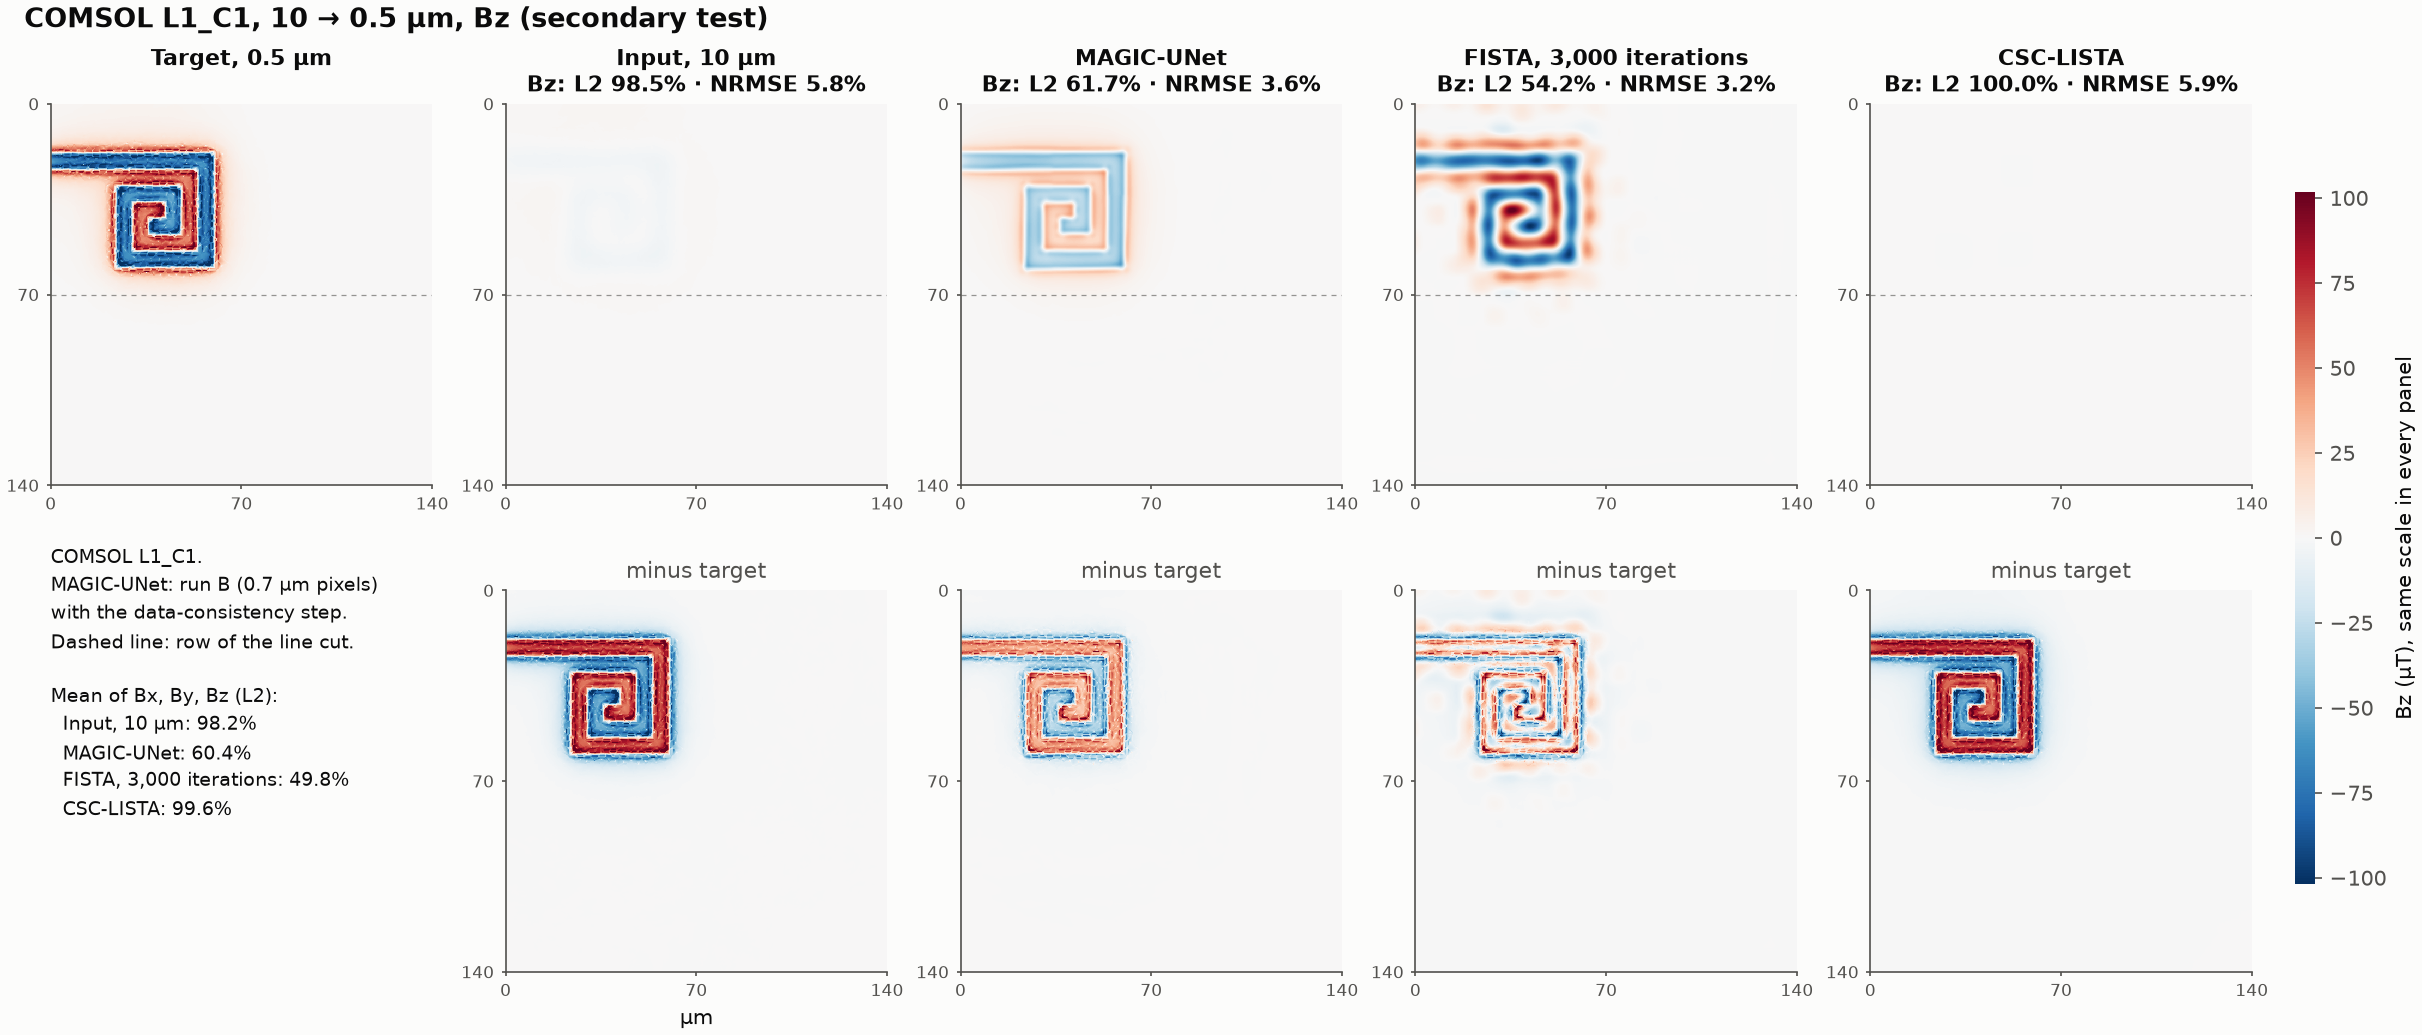
\includegraphics[width=\textwidth]{hs_comsol_L1_C1_maps}
\caption{COMSOL \code{L1_C1}, 10\um\ to 0.5\um. MAGIC-UNet draws the coil in the right place, but too faint.}
\label{fig:hs_comsol}
\end{figure}

\section{Shape and strength, measured separately}

Figure~\ref{fig:hs_comsol} suggests that MAGIC-UNet has the right picture at the wrong brightness. One relative error
cannot tell those apart, so two more numbers are computed:

\begin{code*}{k0_check.py}
        out[f'amp_{c}'] = float(dot[i] / tt[i])
        out[f'cos_{c}'] = float(dot[i] / np.sqrt(pp[i] * tt[i]))
\end{code*}

\code{dot} is the sum of output times target, \code{tt} of target squared, \code{pp} of output squared.
\begin{itemize}
\item \textbf{Amplitude} (\code{amp}): how strong the output is along the target. 1 means the right strength.
\item \textbf{Cosine} (\code{cos}): how alike the two patterns are, whatever their strength. 1 means the same shape.
\end{itemize}

\begin{center}
\begin{tabular}{lccc}
\toprule
COMSOL, C1 family, 10\um\ to 0.5\um & Error & Amplitude & Cosine \\
\midrule
MAGIC-UNet & 59.6\% & 0.42 & 0.95 \\
FISTA, 3{,}000 iterations & 50.2\% & 0.66 & 0.87 \\
\bottomrule
\end{tabular}
\end{center}

MAGIC-UNet has the better shape and less than half the strength. Its COMSOL error is mostly amplitude.

\section{Testing the suspect}

Chapter~\ref{ch:comsol} gives a suspect. COMSOL's field decays faster than physics allows, so its 10\um\ field is weaker
than anything the network was trained on. A weaker field looks, to the network, like a weaker current.

This can be tested without COMSOL. The simulator has the switch of Chapter~\ref{ch:comsol}. Render the same 50 test
layouts again with COMSOL's extra decay in the 10\um\ input, and change nothing else:

\begin{code*}{k0_check.py}
        settings = dict(sim.settings, z_input=Z_IN, z_target=Z_TG, decay_k0=float(k0))
\end{code*}

The reference plane of the switch is 0.5\um, so the target is unchanged; only the input gets weaker. Nothing is
retrained. The rule for reading the result was written first (amendment A5): at the fitted $k_0=0.10$, an error of 45\%
or more means the decay explains most of the gap, 25\% or less means it does not, and in between it explains part.

\begin{center}
\begin{tabular}{lcccc}
\toprule
Extra decay $k_0$ (rad/\um) & MAGIC-UNet error & Amplitude & Cosine & Estimated height \\
\midrule
0 (free space) & 15.8\% & 0.98 & 0.99 & 9.80\um \\
0.05 & 20.7\% & 0.83 & 0.99 & 9.48\um \\
\textbf{0.10 (fitted to COMSOL)} & \textbf{42.0\%} & 0.59 & 0.99 & 8.93\um \\
0.15 & 61.1\% & 0.39 & 0.98 & 8.36\um \\
\midrule
COMSOL, C1 family & 59.6\% & 0.42 & 0.95 & 8.3--8.5\um \\
\bottomrule
\end{tabular}
\end{center}

With no extra decay the check reproduces the saved scores exactly. FISTA, on the 5 layouts it was run on, moves from
47.9\% to 49.4\%.

\begin{figure}[H]
\centering
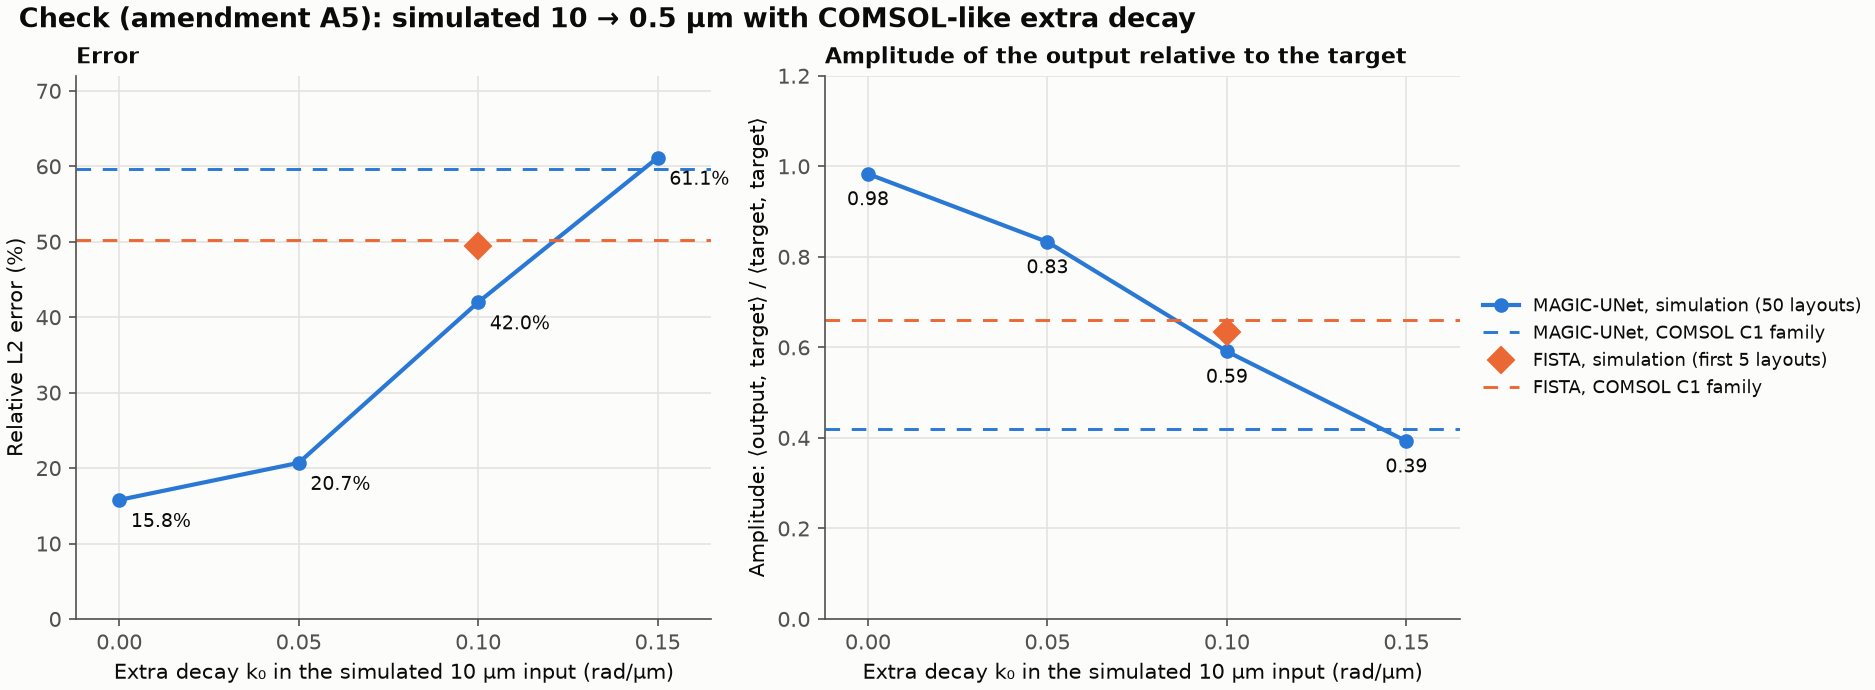
\includegraphics[width=\textwidth]{hs_k0_check}
\caption{MAGIC-UNet and FISTA on simulation as COMSOL-like extra decay is added. Dashed lines: each method's value on
the COMSOL C1-family coils.}
\label{fig:hs_k0}
\end{figure}

\begin{keyidea}[What the check shows]
\begin{itemize}
\item \textbf{The extra decay explains part of the gap:} about 26 of the 44 points between 15.8\% and 59.6\%, at the fitted
$k_0$. The other 18 are not explained.
\item \textbf{It does not flip the order.} At $k_0=0.10$ MAGIC-UNet is still ahead of FISTA (43.4\% against 49.4\% on the
same 5 layouts).
\item \textbf{The error it causes is of the same kind as on COMSOL:} right pattern, weak amplitude, low height estimate.
\item \textbf{MAGIC-UNet is sensitive to the physics of the measurement, and FISTA is not.} FISTA moves by 1.5 points,
MAGIC-UNet by 26. A learned prior inherits the physics of its training data.
\end{itemize}
\end{keyidea}

This also settles the loose end of Chapter~\ref{ch:height}. Run 3 read COMSOL heights too \emph{low} at large standoffs,
and on simulation too high. The last column shows why: extra decay makes a network read a smaller height.

\begin{careful}[What the check does not show]
At $k_0=0.15$ all three numbers land close to their COMSOL values, and 0.15 is inside the range estimated for COMSOL
(0.07--0.17). But it is not the fitted value, and FISTA was not run there. Treat it as a hint. The check also leaves
out COMSOL's walls, its mesh noise and the coil shapes themselves.
\end{careful}

\section{CSC-LISTA does not survive the move to 10\um}

You asked for the other learned methods at 10\um\ too. They had only ever been trained for 3\um. So they were trained
again with the same frozen code and the same settings, and only two things changed: the blur in the operator, and the
height at which the training layouts are rendered. For CSC-LISTA (strict, 64 layers, 33.8\% at 3\um):

\begin{center}
\begin{tabular}{lcccc}
\toprule
Training step & 0 (untrained) & 100 & 500 & 1{,}000 \\
\midrule
Validation error, 64 crops & \textbf{89.8\%} & 102.7\% & 119.9\% & 120.9\% \\
\bottomrule
\end{tabular}
\end{center}

Its best checkpoint is the one \emph{before any training}. Training made it worse. The final scores, 91.8\% on simulation
and 98.1\% on COMSOL, are close to doing nothing: the measured input itself is at about 92--98\%.

Two reasons were written down before the run. Recall from Chapter~\ref{ch:csc_lista} that each layer has a learned
filter $W$, started from the blurred dictionary and cut to a fixed size:

\begin{code*}{csc_lista.py}
        # ISTA start: w = d / L, truncated to the filter support.
\end{code*}
\begin{code*}{csc_lista.py}
            rows.append(full[..., :width, :width] * step)
\end{code*}

\code{width} is 155 pixels, 15.5\um. At 3\um\ the blur is about 4\um\ wide and fits easily. At 10\um\ the blur is as
wide as the filter itself, so cutting it off throws away much of what it should contain, and the layers start from the
wrong operator. The second reason: 64 layers are 64 iterations, and the previous section showed that plain FISTA on the
same dictionary needs about 3{,}000 here.

\begin{careful}
This is a statement about CSC-LISTA \emph{as configured for 3\um}, with only the standoff changed, as you asked. Wider
filters or more layers were not tried, and the run already used 40 of the GPU's 49\,GB. FISTA-Net has only 7 layers; it
is still training and may fail in the same way.
\end{careful}

\section{What can be claimed}

\begin{keyidea}[The fair summary at 10\um]
On free-space simulated data, MAGIC-UNet with a tile matched to the blur reconstructs the 0.5\um\ field from 10\um\ with
15.8\% error, three times better than a converged FISTA, without being told the standoff, and one model covers
6--14\um. On COMSOL at 10\um\ it does \textbf{not} beat FISTA. Part of that is COMSOL's own physics; the rest is open.
\end{keyidea}

\begin{defend}[If your professor asks: 15\% at 10\um\ sounds too good. Is it real?]
It is real on its test set, and the test set is honest about what it is: new layouts from the simulator that made the
training data. The export for the figures reproduced every saved score. It shows that a source prior can recover what
the measurement lost, when the sources look like the training sources. It does not show that the number holds for a
device with other wire shapes or currents.
\end{defend}

\begin{defend}[If your professor asks: then why believe the simulation and not COMSOL?]
Because of Chapter~\ref{ch:comsol}. Above about 4\um\ COMSOL's field breaks Amp\`ere's law in empty air by 27--52\%, and
our simulator matches exact Biot--Savart to under 1\%. But do not hide the COMSOL result. Report both, and report the
check that explains part of the difference.
\end{defend}

\begin{defend}[If your professor asks: what is the weakness of the learned method?]
It depends on the physics it was trained on. A field that decays a little faster than its training fields costs it 26
points, where FISTA loses 1.5. The good news is that the failure announces itself: the output keeps its pattern but
loses strength, and the height read-out drops.
\end{defend}

\begin{defend}[If your professor asks: is the comparison with FISTA fair?]
FISTA has every advantage we could give it: the true standoff, a dictionary learned on the same simulator, and its
penalty, padding and depth all chosen on simulation. MAGIC-UNet trained on 4{,}800 layouts and sees three components at
once. Each has one seed.
\end{defend}

\section{What is not yet known}

\begin{itemize}
\item FISTA-Net at 10\um: training, about 27 hours.
\item The 18 points of MAGIC-UNet's COMSOL gap that the extra decay does not explain.
\item Whether the result holds for other wire shapes, other currents, or a second seed.
\item Whether a re-solved COMSOL model, without the extra decay, would put MAGIC-UNet ahead.
\item Everything on experimental QDM data. Nothing here has been measured.
\end{itemize}

\chapter{Where the review says to go next}\label{ch:next}

Chapter~\ref{ch:review} covered what the review found. This chapter covers what it recommends: what the output of a
paper should be, what each kind of prior can learn, which kinds of generalisation are still untested, how to add
uncertainty, and the method it proposes. Nothing here has been built yet. It is the map for after the evaluation.

\section{Which output should come first}

The project has always treated the field at 0.5\um\ as the goal, and the current as a step on the way. The review argues
for the reverse.

\begin{itemize}
\item The 0.5\um\ field and the equivalent sheet current carry the \emph{same} information. Chapter~\ref{ch:magic} showed
that one follows from the other by exact physics.
\item But only the current can be checked in a real experiment: against the lithography mask that made the wires, and
against the current that was driven through them.
\item A 0.5\um\ field on a 0.1\um\ grid can never be measured on a real QDM. Its optical resolution is of the order of the
wavelength of light.
\end{itemize}

\begin{keyidea}
A paper whose ground truth can never exist outside a simulation is hard to defend at a physics venue. Report the
current as the primary result, and the near field as a consequence of it.
\end{keyidea}

\section{What each kind of prior learns}

Chapter~\ref{ch:limits} showed that methods differ only in the prior band. So the question is what each prior knows.

\begin{center}
\small
\begin{tabularx}{\textwidth}{>{\raggedright\arraybackslash}p{3.6cm}X}
\toprule
Prior & What it knows \\
\midrule
Field-domain dictionary (FISTA, CSC-LISTA) & 32 atoms, each a 7.5\um\ patch of field at 0.5\um. Fields of wires are smooth and
overlap, so many atoms are needed everywhere, the codes come out dense, and the prior is weak \\
Current-domain network (MAGIC-UNet) & Currents are compact, piecewise constant, of one amplitude and continuous. That is a
much stronger statement, and it supports filling in detail past $k_c$ \\
\bottomrule
\end{tabularx}
\end{center}

\begin{careful}[The open question]
Is the network recovering structure, or recalling the simulator's shapes? Both test coils are rectangular spirals of the
simulated width. Until it is tested on something outside the simulator's families (curves, diagonals, pads, two current
levels, two layers), there is no evidence either way. Chapter~\ref{ch:ten_results} makes this question sharper, not
smaller.
\end{careful}

One product no other method offers, and it is cheap: for each reconstruction, report which frequencies were supported
by the data (below $k_c$, for the estimated height and noise) and which came from the prior. That is a direct answer to
``how do you handle the ambiguity''.

\section{Which kinds of generalisation are tested}

\begin{center}
\small
\begin{tabularx}{\textwidth}{>{\raggedright\arraybackslash}p{3.4cm}>{\raggedright\arraybackslash}p{2.2cm}X}
\toprule
Axis & Tested? & Status on 16 November \\
\midrule
Standoff, known & Partly & FISTA at 3 and 10\um \\
Standoff, unknown & Partly & Run 2 in 2--4\um; run 3 across 1--10\um; run B across 6--14\um\ on simulation \\
Geometry & No & Two shapes, both in the simulator's families \\
Wire width, thickness & No & \\
Field of view & No & Fixed 140\um\ image \\
Pixel pitch & No & 0.1\um\ input; the network works at 0.2 or 0.7\um\ after averaging \\
Noise level and type & No & One synthetic family; no sensor noise \\
Current amplitude & Implicitly & Each tile is scaled by its own maximum; one current in all data \\
Real measurement & No & \\
\bottomrule
\end{tabularx}
\end{center}

\section{Magnetostatics has no ruler}

This is the most useful idea in the review's recommendations, and you have already seen a rough version of it.

Look at the blur, $e^{-k\,\Delta z}$. If you double every length in the problem, $k$ halves and $\Delta z$ doubles, and the
product $k\,\Delta z$ does not change. So a 2\um\ wire seen from 10\um\ is exactly the same picture as a 1\um\ wire seen
from 5\um, drawn at a different scale. The physics has no built-in length.

\begin{keyidea}[What follows]
Resample every input so that the standoff is a fixed number of \emph{pixels}. Then every standoff becomes the same problem,
with only the wire width in pixels changing. One network trained at that one normalised standoff would serve every
physical standoff, and every pixel pitch too.
\end{keyidea}

Now look back at Chapter~\ref{ch:ten}. Run B's 0.7\um\ pixels did a crude version of exactly this. Run 2 saw a 3\um\
standoff as 15 pixels of 0.2\um. Run B sees a 10\um\ standoff as about 14 pixels of 0.7\um. That is why the same network,
unchanged, works at 10\um\ once the pixels are scaled: in pixels, it is nearly the problem it already knew how to solve.
The full idea needs a height hypothesis to resample with, and the height search below provides one.

\section{Uncertainty, in order of cost}

Nothing in the project outputs an uncertainty yet. From cheapest to most expensive:
\begin{enumerate}
\item \textbf{Seeds.} The spread of scores over several trained copies, and a per-pixel spread of their outputs. Three
seeds exist at 3\um\ (Chapter~\ref{ch:consistency}).
\item \textbf{A height interval.} Plot the data misfit against the hypothesised height, report the range of heights that
fit about equally well, and check on simulated data how often the true height falls inside it.
\item \textbf{The data-supported and prior-filled bands} of the previous section.
\item \textbf{Conformal intervals,} calibrated on simulated data and then checked on COMSOL and real data. Expect them to
break under the gap between simulator and reality; reporting that honestly is useful in itself.
\item \textbf{Posterior samples} from a diffusion prior (candidate B below), for a machine-learning venue.
\end{enumerate}

\section{Physics errors a learned model could absorb or hide}

A network trained on wrong physics does not complain. It quietly learns the error. The review lists the ones to watch:
\begin{itemize}
\item COMSOL's extra decay. A network trained on COMSOL fields would learn it silently. Keeping it out of the simulator
was right, and Chapter~\ref{ch:ten_results} showed what it does to a network that never saw it.
\item The quarter-turn of COMSOL's components. Now traced to the export (Chapter~\ref{ch:comsol}).
\item Mesh noise shared between configurations. Harmless while COMSOL stays out of training; a leak the moment it enters.
\item Sheet currents against conductors of finite thickness, the thickness of the NV layer, and optical blur on a real
QDM. All three act like extra standoff (Chapter~\ref{ch:limits}).
\item MAGIC-UNet's current does not have to conserve charge, because $J_x$ and $J_y$ come from separate decoders.
\item Scaling each tile by its own maximum hides the absolute strength from the network, and makes empty tiles pure
noise. The run 1 bug was a symptom of this.
\item Zero padding, where COMSOL's walls force the normal field to zero.
\end{itemize}

\section{The method the review recommends}

\textbf{Method A: a data-consistent current-domain solver with a search over height.} Five parts, each with a published
ancestor:

\begin{enumerate}
\item \textbf{Unknown: a stream function $g$}, one scalar image, with the current $J=\nabla\times(g\,\hat z)$. Then the
current conserves charge by construction, and $B_x$, $B_y$, $B_z$ at any height follow from $g$ by the Fourier relations
already in \code{simulate_fields.py}.
\item \textbf{Scale normalisation:} resample the input so the hypothesised standoff is a fixed number of pixels (the
section above).
\item \textbf{Network:} a MAGIC-UNet-style encoder and decoder with one output, $g$, used as the learned prior inside a few
unrolled stages. Each stage alternates the closed-form data-consistency step of Chapter~\ref{ch:consistency}, on all
three components, with a learned correction to $g$, in the manner of USRNet. Tiles at least 8 standoffs wide.
\item \textbf{Height:} an outer search. For each candidate height on a grid, resample, reconstruct, then score by the data
misfit and by how much the network had to correct. Report the best height, the interval where the score stays within
a calibrated tolerance, and one reconstruction per supported height when the interval is wide.
\item \textbf{Training:} the simulator with wider variety: curved and diagonal wires, widths over a decade, two current
levels, finite thickness, white and correlated noise, optical blur. COMSOL and real data stay test-only.
\end{enumerate}

\begin{keyidea}[Why this method, for this project]
\begin{itemize}
\item The one experiment we have points to it: one data-consistency step after MAGIC-UNet took 27.0\% to 24.3\%.
\item The run 3 failure and the read-out test of Chapter~\ref{ch:height} say the height must be chosen by
\emph{reconstructing at each candidate height}, not by re-projecting one prediction. Part 4 does exactly that.
\item Every block has a published ancestor (MAGIC-UNet, USRNet, stream-function priors, the joint distance fit of
Setescak et al.), which respects the rule of published parts with a clearly labelled contribution.
\item It reuses the simulator, the Biot--Savart code and the MAGIC-UNet port.
\end{itemize}
\end{keyidea}

The candidates it was compared with:

\begin{center}
\small
\begin{tabularx}{\textwidth}{l>{\raggedright\arraybackslash}X>{\raggedright\arraybackslash}p{3.6cm}}
\toprule
 & Candidate & Verdict \\
\midrule
A & The method above & Build it \\
B & A diffusion prior on $g$, sampled so that it agrees with the measurement, with the height as a variable & Uncertainty
comes naturally, but training is slow and guidance through such a steep blur is unstable. A second paper \\
C & A Fourier neural operator & No clear advantage over a CNN after resampling \\
D & An untrained network with the exact physics as its loss, height as a free parameter (Dubois et al.) & No simulator gap
at all. Build it anyway as a baseline \\
E & Classical total variation on the stream function, at a grid of heights & A baseline and the identifiability test in
one. Build it anyway \\
\bottomrule
\end{tabularx}
\end{center}

\section{The one claim a paper could make}

\begin{keyidea}[The claim, as the review writes it]
The standoff of a magnetic image can be inferred, with an honest interval, from the image itself once a learned current
prior and exact field physics are combined. Doing so gives better current and near-field reconstructions than methods
that are told the standoff, across a tenfold range of standoffs, and the reconstruction states which part of it the data
support.
\end{keyidea}

What a reviewer would demand, and what exists: baselines (Fourier inversion, total variation on the stream function, an
untrained network, MAGIC-UNet as published, FISTA; we have the last two); data sets (held-out simulated families, ten or
more new finite-element geometries with correct physics, one real QDM measurement with a calibrated standoff; we have two
shapes with an anomalous decay); ablations of every ingredient; three or more seeds; and a test protocol written before
the final runs. The review's realistic venues are Physical Review Applied or IEEE Transactions on Computational Imaging,
with a real measurement.

\section{The five biggest risks}

\begin{enumerate}
\item \textbf{The benchmark is not valid evidence.} Two shapes, a non-physical decay, inconsistent components, a noisy
target. Fix the data before comparing methods further; a real measurement for the paper.
\item \textbf{The learned prior has memorised the simulator's shapes and widths.} Every gain so far is on coils the
simulator was built around. Test on held-out families and new shapes, and keep the untrained-network and total-variation
baselines next to every result, since they have nothing to memorise.
\item \textbf{The height is not identifiable tightly enough to be useful.} The valley is shallow at 3\um\ and will be
shallower higher up, and width and thickness bias it. Report an effective standoff with an interval. Keep the fallback
paper in view: reconstruction given a calibrated standoff, with its sensitivity to errors in that standoff.
\item \textbf{The novelty is thinner than it looks.} MAGIC-UNet already maps field to current, possibly over a standoff
range; Setescak et al.\ already fit the sensor distance jointly. Re-read both in full.
\item \textbf{Statistical fragility.} One seed, many variants on 15 pairs, choices informed by earlier scores. Write the final
protocol first, freeze a new test set no method has seen, use three seeds, and report every run.
\end{enumerate}

A sixth, practical one: one GPU and one person. Method A fits that budget; a diffusion prior and a wide architecture
search do not.

\begin{defend}[If your professor asks: what would you do with three more months?]
Build method A: a stream-function output so the current conserves charge, inputs resampled so the standoff is a fixed
number of pixels, a learned prior inside a few data-consistency steps, and a search over height that reconstructs at
each candidate and reports an interval. Test it on new geometries and on one real QDM measurement with a calibrated
standoff, against an untrained network and total variation, which have no simulator to memorise.
\end{defend}

\begin{defend}[If your professor asks: what is genuinely new here?]
Not learning field to current, not using all three components, and not fitting the distance jointly as an idea: all of
those exist. What is open is inferring the standoff for the whole image with a learned current prior and exact physics,
the one-sided analysis of the ambiguity with a measured height resolution, and a reconstruction that says which
frequencies came from the data and which from the prior.
\end{defend}

\appendix
\chapter{Glossary}

\begin{longtable}{>{\raggedright\arraybackslash}p{3.6cm}>{\raggedright\arraybackslash}p{11.4cm}}
\toprule
Term & Meaning \\
\midrule
\endhead
Adjoint & The transpose of an operator. For a convolution it is the 180-degree rotated filter \\
Atom & One small image in a dictionary, $g_m$ \\
Checkpoint & A saved copy of a model. Also a separate memory trick in \code{torch.utils.checkpoint} \\
Code & A map $x_m$ saying where and how strongly to stamp atom $m$ \\
COMSOL & The finite-element simulation we use as test data \\
Density & Fraction of code values that are not exactly zero \\
Dictionary & The set of atoms \\
Epoch & One pass over the training data. Here, 600 crops \\
FISTA & ISTA plus momentum \\
Ill-posed & A problem where the data alone does not fix the answer \\
ISTA & Gradient step plus shrink, repeated \\
Lasso & Least squares plus an $\ell_1$ penalty \\
LISTA & ISTA unrolled into layers with learned weights \\
Mask & An array of 0s and 1s that hides the padding \\
NRMSE & Root mean square error divided by the target's range \\
Plain & Eq.~20 with no threshold floor \\
Relative $L_2$ & $\lVert y-t\rVert_2/\lVert t\rVert_2$, our main score \\
Residual & The mismatch between predicted and measured data \\
Shrink, soft threshold & Move a value toward zero by $\theta$, stopping at zero \\
Sparse (run) & Eq.~20 with a floor on the thresholds, our addition \\
Speckle & Fine mesh noise in COMSOL fields \\
Standoff & Distance between source and sensor \\
Strict & Plain Eq.~20 with MSE, at 32 and 64 layers \\
Unrolling & Turning iterations into network layers \\
Upward continuation & The exact law for how a field changes with height \\
Wiener & $h/(h^2+\mu)$, a one-parameter deblurring filter \\
\bottomrule
\end{longtable}

\chapter{Where everything is}

\section*{Code}

\begin{center}
\begin{tabularx}{\textwidth}{lX}
\toprule
File & Contents \\
\midrule
\code{scripts/simulate_fields.py} & Data generator \\
\code{scripts/plot_simulated.py} & Realism report \\
\code{scripts/csc_lista.py} & Operator, ISTA, FISTA, dictionary learning, CSC-LISTA, Wiener \\
\code{scripts/train_csc_lista.py} & Training and COMSOL scoring \\
\code{scripts/fista_net.py} & FISTA-Net \\
\code{scripts/train_fista_net.py} & FISTA-Net training \\
\code{scripts/score_fista_depths.py} & FISTA at chosen depths, with a $\lambda$ search \\
\code{tests/test_*.py} & 15 simulation, 15 CSC-LISTA and 8 FISTA-Net tests \\
\bottomrule
\end{tabularx}
\end{center}

\section*{Results on the server}

Host \code{abhaychandra@10.129.6.189}, folder \code{~/learning_ker}.

\begin{center}
\begin{tabularx}{\textwidth}{lX}
\toprule
Folder & Contents \\
\midrule
\code{runs/simulated_3_to_05_v3} & Dataset \\
\code{runs/csc_lista_v2/dictionary_strong} & Three dictionaries; $\lambda=0.3$ is used \\
\code{runs/csc_lista_v2/full_plain} & Plain, 16 layers, with ISTA and FISTA baselines \\
\code{runs/csc_lista_v2/full_sparse} & Sparse MSE, 16 layers \\
\code{runs/csc_lista_v3/relative_16} & Sparse relative, 16 layers \\
\code{runs/csc_lista_v3/relative_32} & Sparse relative, 32 layers \\
\code{runs/csc_lista_strict/layers_32} & Strict, 32 layers \\
\code{runs/csc_lista_strict/layers_64} & Strict, 64 layers \\
\code{runs/csc_lista_lfista/layers_32} & Job 3 \\
\code{runs/fista_net/run_1} & FISTA-Net run 1 \\
\code{runs/fista_net/run_2} & FISTA-Net run 2 \\
\code{runs/fista_net/run_2_interim_step4800} & Interim score of run 2 \\
\code{runs/fista_depths} & FISTA at 32, 64 and 300, first grid \\
\code{runs/fista_depths_lambda} & FISTA at 32, 64 and 300, wider grid \\
\bottomrule
\end{tabularx}
\end{center}

\section*{This booklet}

\begin{itemize}
\item \code{booklet/main.tex} is the main file, with one file per chapter in \code{booklet/chapters}.
\item \code{booklet/make_figures.py} redraws the figures.
\item \code{booklet/check_snippets.py} confirms that every code block still matches the repository.
\end{itemize}

\chapter{References}

\begin{enumerate}
\item J. Liu, X. Chen, Z. Wang and W. Yin, ``ALISTA: Analytic Weights Are As Good As Learned Weights in LISTA'',
ICLR 2019.
\item K. Gregor and Y. LeCun, ``Learning Fast Approximations of Sparse Coding'', ICML 2010.
\item A. Beck and M. Teboulle, ``A Fast Iterative Shrinkage-Thresholding Algorithm for Linear Inverse Problems'',
SIAM Journal on Imaging Sciences, 2009.
\item T. Moreau and J. Bruna, ``Understanding Trainable Sparse Coding via Matrix Factorization'', ICLR 2017,
arXiv 1609.00285.
\item J. Xiang, Y. Dong and Y. Yang, ``FISTA-Net: Learning a Fast Iterative Shrinkage Thresholding Network for
Inverse Problems in Imaging'', IEEE Transactions on Medical Imaging, arXiv 2008.02683. Code:
\url{https://github.com/jinxixiang/FISTA-Net}.
\end{enumerate}


\end{document}
